%%%%%%%%%%%%%%%%%%%%%%%%%%%%%%%%%%%%%%%%%
% Thin Sectioned Essay
% LaTeX Template
% Version 1.0 (3/8/11)
%
% This template has been downloaded from:
% http://www.LaTeXTemplates.com
%
% Original Author:
% Nicolas Diaz (nsdiaz@uc.cl) with extensive modifications by:
% Vel (vel@latextemplates.com)
%
% License:
% CC BY-NC-SA 3.0 (http://creativecommons.org/licenses/by-nc-sa/3.0/)
%
%%%%%%%%%%%%%%%%%%%%%%%%%%%%%%%%%%%%%%%%%

%----------------------------------------------------------------------------------------
%	PACKAGES AND OTHER DOCUMENT CONFIGURATIONS
%----------------------------------------------------------------------------------------

\documentclass[a4paper, 11pt]{report} 
\usepackage{hyperref}

\usepackage[protrusion=true,expansion=true]{microtype} % Better typography
\usepackage{graphicx} % Required for including pictures
\usepackage{wrapfig} % Allows in-line images
\usepackage{tablefootnote} % to display footnotes in tables
\usepackage{threeparttable}
\usepackage[toc,page]{appendix}
\usepackage{multirow}
\usepackage[usenames, dvipsnames]{color}

\usepackage{mathpazo} % Use the Palatino font
\usepackage[T1]{fontenc} % Required for accented characters
\linespread{1.05} % Change line spacing here, Palatino benefits from a slight increase by default

% To have DRAFT displayed accross all pages
%\usepackage{draftwatermark}
%\SetWatermarkText{DRAFT}
%\SetWatermarkScale{1}
%\SetWatermarkLightness{0.95}

\usepackage{background}
\backgroundsetup{
  position=current page.west,
  angle=90,
  nodeanchor=west,
  vshift=-5mm,
  opacity=1,
  scale=4,
  contents=Draft
}

% SPECIAL COMMANDS  

\newcommand{\hls}{HLS\,J0918+5142}
\makeatletter
%\renewcommand\@biblabel[1]{\textbf{#1.}} % Change the square brackets for each bibliography item from '[1]' to '1.'
\renewcommand{\@listI}{\itemsep=0pt} % Reduce the space between items in the itemize and enumerate environments and the bibliography

% TITLE

\renewcommand{\maketitle}{ % Customize the title - do not edit title and author name here, see the TITLE block below
\begin{flushleft} % Right align
{\LARGE\@title} % Increase the font size of the title

\vspace{50pt} % Some vertical space between the title and author name

{\large\@author} % Author name
\\\@date % Date

\vspace{40pt} % Some vertical space between the author block and abstract
\end{flushleft}
}


% NOTATION
%%%%%%%%%%%%%%%%%%%%%%%%%%%%%%%%%%%%%%%%%
\newcommand{\ftone}{f_{\rm{tone}}}
\newcommand{\am}{x}
\newcommand{\elev}{\delta}
\newcommand{\nika}{NIKA2}
\newcommand{\todo}[1]{\textcolor{magenta}{\textbf{#1}}}
\newcommand{\aka}{a.\,k.\,a.}
\newcommand{\wrt}{w.\,r.\,t.}
\newcommand{\bm}{\emph{beammap}}
\newcommand{\bms}{\emph{beammaps}}
\newcommand{\rf}{\emph{RfdIdQ}}
\newcommand{\kidpar}{\emph{kidpar}}
\newcommand{\radec}{\emph{R.\,A.,\,Dec}}
\newcommand{\cm}{\emph{common~mode}}
\newcommand{\cmoneb}{\emph{common~mode~one~block}}

% COMMENTAIRES
%%%%%%%%%%%%%%%%%%%%%%%%%%%%%%%%%%%%%%%%%
\newcommand{\addparag}[1]{ {\color{magenta} $[$ ADD A PARAGRAPH ON: $]$ #1} }


%
% PAGE STYLE
%
\setlength{\textwidth}{16cm}
\setlength{\textheight}{23cm}
\oddsidemargin +0.5cm
\evensidemargin +0.5cm
\topmargin 0.1cm

%\setcounter{secnumdepth}{1}
\setcounter{tocdepth}{1}

\begin{document}

%----------------------------------------------------------------------------------------
%	TITLE
%----------------------------------------------------------------------------------------
\title{\parbox{16cm}{
    \includegraphics[width=5.5cm]{Figures/Logo_NIKA2.pdf} \\ [5mm]   
    \textbf{NIKA2 research note} \\ [5cm]   
    \begin{center}\sf\bfseries\huge
      NIKA2 Commissioning Phase One Results \\ [-4mm]
      \rule{16cm}{1pt}\\ [2cm]   
    \end{center}
    \begin{center} \small
      Prepared by the \emph{NIKA2 Commissioning Tiger team}: \\
      Laurence Perotto,  Nicolas Ponthieu, Juan-F. Mac\'ias-P\'erez,
      F.-Xavier D\'esert, Jean-Fran\c cois Lestrade, Herv\'e Aussel,
      Fr\'ed\'eric Mayet and Florian Ruppin\\ [4cm]     
    \end{center}
    %\hfill
    %\scriptsize Prepared by The NIKA2 Commissioning Tiger team \\ [5cm]
%    September 2018
  }
}
\author{{\textit{NIKA2 collaboration}}  }
\date{\today}

\maketitle % Print the title section
%
%
%

\pagenumbering{roman}

\tableofcontents

\clearpage
\listoffigures
\listoftables

%----------------------------------------------------------------------------------------
%	ABSTRACT AND KEYWORDS
%----------------------------------------------------------------------------------------

%\renewcommand{\abstractname}{Summary} % Uncomment to change the name of the abstract to something else
\newpage
\pagenumbering{arabic}

\begin{abstract}
We present NIKA2 performance assessment after the end of the commissioning in intensity.
\end{abstract}

%\hspace*{3,6mm}\textit{Version:}  % Version

%\vspace{30pt} % Some vertical space between the abstract and first section

\newpage
%----------------------------------------------------------------------------------------
%
%	ESSAY BODY
%
%----------------------------------------------------------------------------------------
%\tableofcontents



%----------------------------------------------------------------------------------------
%	INTRODUCTION
%----------------------------------------------------------------------------------------
\chapter{Total power Commissionning Introduction {\color{blue} Nico}}
\label{se:intro}
%----------------------------------------------------------------------------------------
%	INTRODUCTION
%----------------------------------------------------------------------------------------
%\section{Introduction}
%\label{se:intro}
%
%Submillimetric domain: a unique thorough view of the Universe from
%planetary surfaces in the Solar System to early galaxies,
%high-redshift galaxy clusters and the Cosmic Microwave
%Background (CMB).\\
%Ground-based submillimeter experiments have made tremendous progress in the last
%decades thanks to the advent of large detector arrays, challenging the
%motivation for spatial experiments.\\
%The current experimental efforts are driven by two complementary
%challenges: the improvement of the polarisation sensitivity to detect
%primordial polarisation B-mode of the CMB and measure CMB lensing on
%one hand and on the other hand the increase the angular resolution to
%reveal the inner structure of astrophysical objects, such as
%high-redshift galaxies and galaxy clusters.\\

Sub-millimetric and millimetric domains offer a unique view of the
Universe from nearby astrophysical objects, including planets,
planetary systems, galactic sources, nearby galaxies, to high-redshift
cosmological probes, \emph{e.g.} distant dusty star-forming galaxies,
clusters of galaxies, Cosmic Infrared Background (CIB), Cosmic Microwave
Background (CMB).
%for scientific purposes that ranges from planetary science to cosmology.

Ground-based {\lp continuum} millimeter experiments have made spectacular progress in
the past-two decades thanks to the advent of large arrays of
high-sensitivity detectors~\citep{Wilson2008_AZTEC,
  Siringo2009_LABOCA, Swetz2011_ACT, Bleem2012_SPT, Monfardini2011_NIKA, Holland2013_SCUBA2,
  Dicker2014_MUSTANG2, Adam2017}. %, challenging the
%motivation for spatial experiments.
This fast growth will continue as experimental efforts are
driven by two challenges: improving the sensitivity to the
polarisation to detect the signature of
the end-of-inflation gravitational waves in the CMB, and reaching
arcminute angular resolution to exploit the CMB secondary anisotropies
as cosmological probes, and sub-arcminute resolution to unveil the
inner structure of faint or complex astrophysical objects and to map
the early universe down to the confusion limit. Furthermore, new
generation of sub-arcminute millimetric experiments, like NIKA2, which
combines high angular resolution with a high mapping speed and a large
coverage in the frequency domain, will achieve a breakthrough in 
%will revolutionize
our detailed understanding of the formation and evolution of
structures throughout the Universe.

%
%In particular, it would allow us to study the inner structure of
%galaxy clusters (detected by Planck), and to get a new view on star
%formation at low and high redshift, by studying the role of magnetic
%field at a sub parsec scale in our Galaxy, and mapping the dusty star
%forming galaxies up to redshifts equal to 6.
%
%NIKA2 is a high-resolution large field-of-view multi-thousand detector
%camera in operation at the 30-m IRAM telescope since October 2017. ,
%after a successful commissioning of the instrument. 
%Fourth generation of
%imagers installed at the IRAM 30-m: after the single beam
%imagers, the 7-pixel camera of the late 90's and several versions of
%MAMBO. Unlike its predecessors, NIKA2 is based on KIDs. Validated with
%NIKA pathfinder.\\
%Brief historic of the commissioning. \\
%The instrument commissioning was successfully completed in September
%2017.
%NIKA2 is now open to the scientific community and will operate
%for the next decade.

The New IRAM KID Array Two, NIKA2, is a sub-arcminute-resolution
high-mapping speed camera observing simultaneously a 6.5' diameter
field of view (FOV) in intensity in two
frequency channels centered at 150 and $260\,\rm{GHz}$ and in
polarisation at $260\, \rm{GHz}$~\citep{Adam2018}. NIKA2 was installed
at the IRAM \trentemetre\ telescope in October 2015 with a partial readout
electronics, and operated in the final instrumental configuration since
January 2017. After a successful
commissioning phase that ended in October 2017, NIKA2 is
open to the community for science-purpose observations for the next
decade. NIKA2 will provide key observations both at the galactic scale
and at high redshifts to address a plethora of open questions, including
the environment impact on dust properties, the star formation processes
at low and high redshifts, the evolution of the large-scale structures
and the exploitation of galaxy clusters for accurate cosmology.
%
%NIKA2, which will provide unprecedented maps at low and high
%redshifts, ranging from the interstellar medium to the dusty star
%forming galaxies up to redshifts equal to 6, will be a key experiment
%to address plethora of open questions in astrophysic and cosmology,
%ranging from the understanding of the star formation process at low
%and high redshift to  and accurate cosmology with galaxy clusters 
%

At the galactic scale, progress in understanding the star formation
process relates to an accurate characterization of dust properties in
the interstellar medium (ISM). NIKA2 will provide the high-resolution
high-mapping speed dual-wavelength millimeter observations that are
required for the determination of the mass and emissivity of
statistically significant samples of dense, cold, star-forming
molecular clouds~\citep{Rigby2018}.
Deep multi-wavelengths surveys of nearby galaxies and of large areas
of the galactic plane also allows for setting constraints on
environmental-related variations of the dust properties.
Furthermore, NIKA2 observations are needed for a
detailed study of the inner molecular cloud filamentary structure that
hosts Solar-mass star progenitors~\citep{Bracco2017}, to
understand the evolution process that culminates in star
formation (see \emph{e.g.}~\citet{Andre2014} for a review). Ultimately, these
observations are also helpful to understand planet formation within
proto-planetary disks.

For cosmology, NIKA2 observations will have two major
implications. On the one hand, they represent a unique opportunity to
study the evolution of the galaxy cluster mass calibration with
redshift and {\lp dynamical state} for their accurate exploitation as cosmological probe. 
Galaxy clusters are efficiently detected via the thermal
Sunyaev-Zel'dovich (tSZ) effect~\citep{SZ1970} up to high redshifts {\lp ($z<1.5$)}, as was recently
proven by CMB
experiments~\citep{Hasselfield2013_ACT_SZ, Reichardt2013_SPT_SZ, Planck2016_SZcat}.
The exploitation of the vast SZ-selected galaxy cluster catalogues is
currently the most powerful approach for cosmology with galaxy
clusters~\citep{Planck_2016_SZ_cosmo}. However, the accuracy of the tSZ cluster
cosmology relies on the calibration of the relation between the tSZ
observable and the cluster mass and on the assessment of both its redshift
evolution and the impact of the complex cluster physics on its calibration. 
%Cosmological constraints can be drawn from tSZ-selected cluster
%samples by using either the cluster number counts or the angular power
%spectrum. It requires a high purity sample to avoid bias, and in
%particular the understanding of the distribution of matter within the
%cluster, and the evaluation of the scatter induced by disturbed
%systems in the relation between the tSZ integrated flux and the total
%cluster mass.
Previous arcminute resolution experiments only allowed detailed studies
of the intra cluster medium spatial distribution for low redshift clusters (z <
0.2). Sub-arcminute resolution high mapping speed experiments are
required to extend our understanding of galaxy cluster towards high
redshift~\citep{Tony2019}. \citet{Ruppin2018} has reported the first high-resolution
tSZ mapping of a galaxy cluster with NIKA2. Furthermore, NIKA2
capabilities for the characterization of high-redshift {\lp ($0.5<z<0.9$)} galaxy clusters
has been verified using numerical simulation~\citep{Ruppin2019}.

On the other hand, in-depth mapping of large extragalactic fields with
sub-arcminute resolution with NIKA2 will provide unprecedented insight
on the distant universe. %Combining high mapping speed and sub-arminute
%resolution is mandatory to
Indeed, hundreds of dust-obscured optically-faint galaxies will be
detected up to high redshift
($z \approx 5$) during their major episodes of star formation.
%For this
%purpose, the high-angular resolution, combined with high mapping
%speed, is key to reduce the confusion noise, which is the ultimate
%limit of cosmological surveys~\citep{Bethermin2017_simu}.
{\lp For this purpose, the high-angular resolution is key to reduce the
confusion noise, which is the ultimate limit of cosmological
surveys~\citep{Bethermin2017_simu}, while the high mapping speed allows
this irreducible noise level to be reached in the extragalactic field
map in a short integration time.}
This will help quantifying the star formation at $z \approx 5$, probing the whole
star formation evolution across cosmic ages and clarifying the
role of the dusty galaxies in the reionization of the
universe~\citep{Mancuso2016}. Moreover, NIKA2 observations will be critical for our
understanding of galaxy formation and evolution.

%[ATTENTION COPIE]
%Similarly, distant universe studies via deep surveys will
%benefit from a large instantaneous field-of-view and sensitivity
%to cover sky regions at the confusion limit. This results
%in detecting dust-obscured optically faint galaxies during
%their major episodes of star formation in the early universe
%(B\'ethermin et al. 2017, Geach et al. 2017).\\

The current generation of sub-arcminute resolution experiments also
include the Large APEX Bolometer Camera
(LABOCA~\citep{Siringo2009_LABOCA}) at the Atacama
Pathfinder Experiment (APEX) 12-meter telescope, which covers a
12' diameter FOV at $345\, \rm{GHz}$ {\lp at an angular resolution of about
19''}; AzTEC at the 50-meter Large Millimeter Telescope, which operates with a
single bandpass centered at either 150, 220 or
$270\,\rm{GHz}$~\citep{Wilson2008_AZTEC}, {\lp and which has a beam FWHM of
$18''$ in the latter band}; the Submillimeter Common User Bolometer
Array Two (SCUBA-2~\citep{Holland2013_SCUBA2,Dempsey2013_SCUBA2}) on the
15-meter James Clerk Maxwell Telescope, which simultaneously
images a FOV of about 7' %at $850\, \mu\rm{m}$ ($353\,
%\rm{GHz}$) and $450\, \mu\rm{m}$
%($666\,\rm{GHz}$)
at $353\,\rm{GHz}$ and $666\,\rm{GHz}$ {\lp with a main beam FWHM of 13''
and 8'' in the two frequency channels, respectively}
; MUSTANG-2 at the 100-meter Green Bank telescope,
which maps a 4.35' FOV at 
$90\,\rm{GHz}$ {\lp with 9'' resolution}~\citep{Dicker2014_MUSTANG2, Stanchfield2016_MUSTANG2}.
Therefore, NIKA2 is unique
in combining an angular resolution better than 20'', an instantaneous FOV of a
diameter of 6.5' and multi-band observation capabilities at $150$ and
$260\,\rm{GHz}$.


Most of the other millimeter instruments consists of bolometric cameras. By contrast,
NIKA2 is based on the Kinetic Inductance Detectors (KID)
technology~\citep{Day2003, Doyle2008_LEKID, Shu2018_LEKID}. This concept has been
first demonstrated with a pathfinder instrument,
NIKA~\citep{Monfardini2010_NIKA, Monfardini2011_NIKA}.
Installed at the IRAM 30-m telescope until 2015, NIKA demonstrated
state-of-the-art performance~\citep{Catalano2014}, and obtained
breakthrough results
(see \emph{e.g.},~\citet{Adam2014, Adam2017_kSZ}.
NIKA has been crucial in optimizing the NIKA2 instrument and data
analysis. 

%Key tool for a large variety of astrophysical and cosmological
%purposes, from Kuiper Belt objects or moons in the Solar system to
%high-redshift galaxies and galaxy clusters. The main scientific
%obsjectives are articulated around five ambitious guaranteed-time
%large programs [add a small paragraph per LP]\\
%
%These scientific program requires high performance standard in term of
%mapping capabilities, sensitivity, angular resolution and stability of
%the system. We assess this performance using a large amount of
%technical and science-purpose data acquired since the full
%installation of NIKA2.\\

A thorough description of the NIKA2 instrument is presented in \citet{Adam2018},
along with the results of the commissioning in intensity based on the
data acquired during the two technical campaigns of 2017.
%
{\lp In the present paper, we propose a standard calibration method, which is
referred to as the \baseline\ calibration, to go from raw data to
stable and accurate flux density measurements.} 
%
%The present paper discusses in detail step-by-step data reduction,
%from the observations and raw data to the sensitivities and an
%assessment of the calibration accuracy, thereby discussing the pros
%and cons of different strategies to provide robust results.
%
%In this paper, we
%detail the dedicated procedures that we have developed for the
%calibration.
%We describe a standard calibration method, which is
%referred to as the \baseline\ calibration, but we are also discussing
%the pros and cons of alternative methods, which may in fact in the
%future lead to even better calibration accuracy and stability.
Furthermore we assess the performance in intensity using a large
amount of data acquired between January 2017 and February 2018.
Regarding the performance of the polarization capabilities, their
assessment will be addressed in a forthcoming paper.
To achieve a reliable and high-accuracy estimation
of the performance, we perform extensive testing of the
stability along both the analysis methodological
choices and the observing conditions.
{\lp First, the methodological choices and hypothesis may have an impact on
the performance results and the systematic errors. At each step of the
calibration procedure and for each performance metrics, we compare the
results obtained using the \baseline\ method to alternative approaches to
ensure the robustness against systematic effects.}
Second, we check the stability of the results using a large number of
independent data sets corresponding to variable observing conditions.
%To achieve
%high-accuracy estimation of each key performance characteristics,
%we test their stability against the methodological choices by
%comparing various analysis approaches, and we check their stability
%againts the observating conditions using vast independent data sets.
Specifically, most of the performance assessment relies on data
acquired during the February 2017 technical campaign (N2R9) and the
October 2017 (N2R12) and January 2018 (N2R14) first and second
scientific-purpose observation campaigns. {\lp These observation
campaigns are referred to as the {\emph reference observation campaigns}.}
Each campaign consists of about 1300 observation scans lasting between
two and twenty minutes for a total observation time of about 150 hours. 
%This large data set
%acquired through a year enables for testing against time-evolution and
%observing-dependency of the performance.

%Outlines
This paper constitutes a review of NIKA2 calibration and
performance assessment in intensity. It is intended to be a reference
for observations with NIKA2, which will last at least for ten years. 
The outline of the paper is as follows:
Sect.~\ref{se:instru}~to~\ref{se:dataproc} give short summaries of the
instrumental set up, the observational modes and the data analysis methods
that have been used for the calibration and the performance
assessment. Sect.~\ref{se:geometry}~to~\ref{se:sensitivity} detail the
dedicated calibration methods, extract the key characteristic results
and discuss their accuracy and robustness. The field-of-view
reconstruction and the KID selection for science purpose are discussed
in Sect.~\ref{se:geometry}. The beam pattern is characterized in
Sect.~\ref{se:beam}, along with the main beam
full-width at half maximum and the beam
efficiency. Sect.~\ref{se:opacity} is dedicated to the derivation of
the atmospheric opacity. The methods that we have proposed to
calibrate are gathered in Sect.~\ref{se:calibration}, while
Sect.~\ref{se:photometry} presents the validation of these methods and
the calibration accuracy and stability assessment. The noise
characteristics and the sensitivity are discussed in
Sect.~\ref{se:sensitivity}. Finally, Sect.~\ref{se:summary} summarizes
the main measured performance characteristics and {\lp briefly
describes next steps for future improvements on NIKA2.}
%offers perspectives for their improvements. 

















\clearpage
%----------------------------------------------------------------------------------------
%	GENERALITIES: INSTRUMENT, OBSERVATION AND METHODS
%----------------------------------------------------------------------------------------
\chapter{Intrument, observations and methods}
\label{se:chap_instru_obs_methods}

This chapter is meant to be an introduction to the instrument and the data
reduction from an astronomer point of view. It summarizes the intrument
parameters that are relevant for the data processing and the different steps
required to go from raw data to scientific maps. The details of each of these
parameters and their derivation is the object of the following sections.

%%	INSTRUMENT

\section{Overview of the NIKA2 instrument}

\subsection{Optics}

NIKA2 is a millimeter camera able to simultaneously image a
field-of-view of 6.5\,arcmin at 150 and 260~GHz, with polarimetric
capabilities at 260~GHz using KIDS. A 30-centimeters diameter air-gap
dichroic splits the 150 GHz (reflection) from the 260 GHz
(transmission) beams.  A grid polarizer ensures then the separation of
the two linear polarisations on the 260 GHz channel.  There are
therefore three KIDS array in NIKA2, one at 2mm, two at 1mm. 

%-------------------------
% HERVE
\input{bandpass}
%-------------------------


\subsection{Cryogenics}
Further technical details on the NIKA2 instrument can be found in the
technical paper {\bf REF !}



\subsection{KIDs and electronics}

NIKA2 focal plane is equipped with arrays of Kinetic Inductance
Detectors (KIDs hereafter), which are high-quality factor
superconducting resonators. They are operated at 150~mK that is well
below the critical temperature, which ensures their responsivity
properties ... 

\addparag{LUMPED KIDS}

The 2mm array (150~GHz) consist of 616 pixels
(KIDS), disposed to cover a circle with a 78 mm diameter. Each pixel
has a size of $2.8 \time 2.8 mm^{2}$ . This is the maximum pixel size that can
be adopted without significantly degrading the telescope resolution,
as it corresponds roughly to a 1F$\lambda$ sampling of the focal
plane.  The array is labelled A2 in all the following.

At 1mm, there are two arrays, labelled A1 and A3, consisting of 1140
KIDS with a size of $2 \time 2 mm^{2}$ to ensure a comparable 1F$\lambda$
sampling.


\addparag{NIKEL}


\subsection{KID tuning}

\addparag{$\ftone$ definition}






%% Data reduction: explain what is needed to go from raw timelines to maps.
%% it will be a list of what is needed with very little description that will
%% announce the details on each item that is developped in the following
%% sections.


\section{Overview of the data reduction pipeline}% {\color{YellowGreen} Nico}}
\label{se:pipeline_overview}

Because each matrix of \nika\ is a filled array with more than one
detector per \new{main beam} PSF on average, and because the atmosphere and electronic noise act as
correlated low frequency parasites, the data reduction of \nika\ does not
proceed on an individual KID basis in general. This, in addition to the
necessary pointing information specifies some of the data reduction
process. In short, the data reduction proceeds as such:

\begin{itemize}
\item Low level processing (Sect.~\ref{se:ll_proc})
\item Pointing reconstruction (Sect.~\ref{se:ptg})
\item TOI calibration and opacity correction (Sect.~\ref{se:flux_calib})
\item TOI processing (Sect.~\ref{se:toi_proc})
\item Map projection (Sect.~\ref{se:map_projection})
\item Photometry (Sect.~\ref{se:intro_photometry})
\end{itemize}

\subsection{Low level processing}
\label{se:ll_proc}

A first step of the analysis is to read the data produced by \nika's
acquisition. The data as such comprise various quantities that describe the
variations of the KID's resonance frequencies, such as $I$, $Q$, $dI$,
$dQ$. From these quantities, and throughout this work, we use our so called
\rf\ photometric estimator that combines them into a quantity that is
proportionnal to the flux absorbed by a KID \cite{Calvo13} and homogeneous to Hz.

In addition to this, we look for and remove the - rare - cosmic rays
events. KIDs have such fast time constants that unlike bolometers, these events
affect a sole sample that is easy to detect by a simple comparison to the rms of
the TOI a few second window. These affected samples are remplaced by a simple
linear interpolation of their surrounding (not to leave holes in the TOI) but
are flagged in order not to project false data on the final map.

We also have a series of tests that read flags from the acquisition
overall. These flags monitor potential jumps in the cryostat or acquisition
monitoring. Most important are the flags related to the tuning. Because the
acquisition file boundaries are not strictly linked to the beginning and the end of
a scan, we must discard everything that happens before the last tuning of the
beginning, and everything after the first automatic tuning that happens when the
scan is done.

Because the tuning of KIDs might fail from time to time depending on the weather
conditions for instance, we systematically check each KID and see if its noise
is far from the average noise of all other KIDs in the same array, with a
typical $3\,\sigma$ threshold. This criterion may seem a bit tight, but in any case, KIDs
are inverse noise variance weighted in the final map projection, so they would
be given relatively low weight anyway (see Sect.~\ref{se:map_projection}).

At this stage of the processing, we have isolated the relevant fraction of the
data for scientific processing and flagged out potentially misbehaving KIDs or
timeline accidents (glitches).

\subsection{Pointing reconstruction}
\label{se:ptg}

This step consists in addressing each sample of each KID to the correct sky
coordinates and their associated map pixel. The pointing data are passed to the
\nika\ raw data. They describe the absolute
pointing of a reference point in the focal plane in various quantities, the
absolute azimuth and elevation $(\alpha,\delta)$ of the source, together with
offsets $(\Delta\alpha_t, \Delta\delta_t)$ \wrt~these. Because our final maps
will be centered on a fixed position (typically the center of the source that is
aimed by the focal plane reference position), we are especially interested in
pointing offsets \wrt~this position. We therefore detail here the derivation of
these offsets.

We store KID pointing offsets \wrt\ the reference position in Nasmyth $(x,y)$
coordinates (independent of time) once and for all in our KID database
(\aka~\kidpar). Sect.~\ref{se:fp_reconstruction} details how these offsets are
derived. To go from Nasmyth offsets to $(\alpha,\delta)$ offsets, we apply the
following rotation by the elevation angle:

\begin{eqnarray}
\Delta\alpha^k_t &=&  \cos\delta_t \Delta x^k + \sin\delta_t \Delta y^k, \nonumber\\
\Delta\delta^k_t &=& -\sin\delta_t \Delta x^k + \cos\delta_t \Delta y^k, \nonumber
\end{eqnarray}

where $k$ is a KID index. Adding these offsets to the reference $(\Delta
\alpha_t, \Delta \delta_t)$ gives the absolute pointing of each KID in these
coordinates. An extra rotation by the parallactic angle $\eta_t$ is required to
obtain KID's coordinates in \radec\ coordinates:

\begin{eqnarray}
\Delta R.\,A.^k_t &=&  \cos\eta_t \Delta\alpha^k_t + \sin\eta_t \Delta\delta^k_t,\\
\Delta Dec^k_t    &=& -\sin\eta_t \Delta\alpha^k_t + \cos\eta_t \Delta\delta^k_t.
\end{eqnarray}

We now have the pointing of each KID at each time relative to the source that we
usually center on our final map. It then trivial to assign the map pixel
corresponding to this pointing on a Nearest Grid Point basis.

This pointing reconstruction is done early in the data reduction process because
we'll need to know when a KID is close or far from the source for the timeline
processing (Sect.~\ref{se:toi_proc}).

\subsection{TOI calibration}
\label{se:flux_calib}

We now focus on the absolute calibration of each TOI. As stated in
Sect.~\ref{se:ll_proc}, at this stage of the reduction each KID \rf~timeline is
in Hz. The conversion process to go from these Hz into Jy/beam proceeds in two
steps: a standard absolute calibration and a correction for the current opacity
and elevation.

The standard conversion from Hz to Jy/beam is stored in the
\kidpar\ database. The derivation of these gains $g(k)$ is detailed in
Sect.~\ref{se:fp_reconstruction}. Suffice is to say here that simply multiplying
the TOI's by these gains converts them into Jy/beam. Of course, this individual
absolute calibration also acts as a relative calibration. This calibration is
meant to work at zero opacity and 90$^\circ$ elevation. We thus need to correct
for the current opacity $\tau$ and elevation. In short, the absolute calibration reads

\begin{equation}
TOI^k(t) [{\rm Jy/beam}] = \rf^k(t)[{\rm Hz}] \times g(k) \times e^{\tau_t/\sin\delta_t}
\end{equation}

The derivation of opacity is presented in Sect.~\ref{se:opacities}.

\subsection{TOI processing}
\label{se:toi_proc}

\begin{figure}[ht!]
\begin{center}
\includegraphics[clip, angle=0, scale=0.4]{Figures/toi_plot.eps}
\includegraphics[clip, angle=0, scale=0.4]{Figures/toi_plot_decorr.eps}
\caption[Example of Time-Ordered-Information]{\emph{Left:} Example of 40 KID raw timelines during an observation
  of Uranus. The low frequency correlated component (atmosphere and electronic
  noise) is clearly seen. \emph{Right:} One of these TOIs and the scaled
  \cm\ that is subtracted from it.}
\label{fig:nika_toi}
\end{center}
\end{figure}

\begin{figure}[ht!] % Inline image example
\begin{center}
\includegraphics[width=0.3\textwidth]{Figures/NoiseTests/corrmat_TOI_array_1_20170228s151.pdf}
\includegraphics[width=0.3\textwidth]{Figures/NoiseTests/corrmat_TOI_array_2_20170228s151.pdf}
\includegraphics[width=0.3\textwidth]{Figures/NoiseTests/corrmat_TOI_array_3_20170228s151.pdf}
\includegraphics[width=0.3\textwidth]{Figures/NoiseTests/corrmat_TOI_CM_array_1_20170228s151.pdf}
\includegraphics[width=0.3\textwidth]{Figures/NoiseTests/corrmat_TOI_CM_array_2_20170228s151.pdf}
\includegraphics[width=0.3\textwidth]{Figures/NoiseTests/corrmat_TOI_CM_array_3_20170228s151.pdf}
\includegraphics[width=0.3\textwidth]{Figures/NoiseTests/corrmat_TOI_PCA_array_1_20170228s151.pdf}
\includegraphics[width=0.3\textwidth]{Figures/NoiseTests/corrmat_TOI_PCA_array_2_20170228s151.pdf}
\includegraphics[width=0.3\textwidth]{Figures/NoiseTests/corrmat_TOI_PCA_array_3_20170228s151.pdf}
\includegraphics[width=0.3\textwidth]{Figures/NoiseTests/corrmat_TOI_BCP_array_1_20170228s151.pdf}
\includegraphics[width=0.3\textwidth]{Figures/NoiseTests/corrmat_TOI_BCP_array_2_20170228s151.pdf}
\includegraphics[width=0.3\textwidth]{Figures/NoiseTests/corrmat_TOI_BCP_array_3_20170228s151.pdf}
\end{center}
\caption[KID-to-KID correlation matrices]{\emph{From left to right:} TOI correlation
  matrices for the three NIKA2 arrays (A1, A2, and A3) for scan
  20170228s150. From top to bottom we present the correlation of the raw data,
  after CM, PCA and MCP decorrelation methods. \label{corrmatrix}}
\end{figure}

As presented on Fig.~\ref{fig:nika_toi}, the atmosphere and the electronic noise
combine into a large low frequency component that we want to eliminate as much
as possible. Most of the atmospheric component is common to all KIDs, which is
expected because the telescope is a $30\,\rm{m}$ dish and therefore
has a near field limit at 900\,km. 

On Fig.~\ref{fig:nika_toi}, the planet Uranus is visible in the TOIs and serves as
guide to both the noise relative amplitude and the discussion about TOI
processing in the following. On Fig.~\ref{corrmatrix}, we take a scan on Pluto
where the signal is negligible compared to noise on the timescale of a scan to
focus on the noise properties. We present the KID to KID timeline correlation
matrices for the three arrays, either before any data reduction or with
different estimates of the low frequency component:

\begin{itemize}
\item {\bf Common Mode decorrelation (CM)}. We use all detectors of the same
  array to build an average low frequency component nicknamed \emph{common
    mode}. This mode is then linearly regressed and subtracted from each KID
  timeline. In this method, the \emph{common mode} at time $t$ is the median of
  all KIDs at this time $t$.

\item {\bf Principal Component Analysis (PCA)}. For each NIKA2 array
  independently we decompose the covariance matrix in principal components. From
  those we derive up to 10 independent templates corresponding to the largest
  eigenvalues that we subtract from the TOIs.

\item {\bf Most correlated pixels (\cmoneb)}. For each detector in a given array we
  identify the detectors that are most correlated to it (a minimum of
  15). Using those detectors we compute a common mode like in method CM but with
  more refinements to be valid even on bright sources (see below).
\end{itemize}

As expected the raw data
noise correlation is dominated by atmospheric noise and we observe full
correlation between detectors but for badly behaving detectors which are removed
from the analysis. Significant residual correlation and anti-correlation is
observed after CM decorrelation. This is both due to spatial changes in the
atmospheric emission (overall residuals) and to instrumental and electronic
noise characteristics (correlation blocks that can be associated to electronic
boxes).  The PCA decorrelation leads to approximately block-diagonal correlation
matrices. These observed blocks in the correlation matrix can be associated to
first order to the different sub-bands in each of the electronic boxes. In the
case of the MCP decorrelation, for which only those pixels highly correlated to
the pixel of interest are used, we observe that the correlation matrix is more
diagonal as in the two other derivations of the common mode.

\begin{figure}[ht!] % Inline image example
\begin{center}
\includegraphics[clip=true, trim={0.5cm, 0, 0, 0.6cm},width=0.32\textwidth]{Figures/NoiseTests/rms_TOI_array_1_20170228s151.pdf}
\includegraphics[clip=true, trim={0.5cm, 0, 0, 0.6cm},width=0.32\textwidth]{Figures/NoiseTests/rms_TOI_array_2_20170228s151.pdf}
\includegraphics[clip=true, trim={0.5cm, 0, 0, 0.5cm},width=0.32\textwidth]{Figures/NoiseTests/rms_TOI_array_3_20170228s151.pdf}
\includegraphics[clip=true, trim={0.5cm, 0, 0, 0.5cm},width=0.32\textwidth]{Figures/NoiseTests/pws_TOI_array_1_20170228s151_mod.pdf}
\includegraphics[clip=true, trim={0.5cm, 0, 0, 0.5cm},width=0.32\textwidth]{Figures/NoiseTests/pws_TOI_array_2_20170228s151_mod.pdf}
\includegraphics[clip=true, trim={0.5cm, 0, 0, 0.5cm},width=0.32\textwidth]{Figures/NoiseTests/pws_TOI_array_3_20170228s151_mod.pdf}
\end{center}
\caption[Noise RMS and power spectra]{From top to bottom and from left to right,
  we show the data rms and power spectra for the three NIKA2 arrays (A1, A2, and
  A3) for scan 20170228s150. The rms and power spectra are given for the raw
  data (blue), and for the CM (green), PCA (red) and MCP (cyan) decorrelated
  data. The vertical lines in the rms noise figures separate detectors from
  different readout electronic boxes. Within each electronic box the pixels are
  ordered with increasing resonant frequency across the electronic
  band. \todo{To enlarge the y- and x- title}
  \label{rmspws}}
\end{figure}

In Fig.~\ref{rmspws} we present the rms noise per KID and the power spectra of
a typical raw datastream, and the CM, PCA and MCP decorrelated data. We observe that after
decorrelation we reduce significantly the rms of the
noise. Equivalently, the $1/f$-like noise in the power spectra
(principally due to atmospheric emission)
is significantly reduced leading to nearly flat spectra down to 0.05 Hz, with
larger $1/f$-like residual noise for the CM decorrelation method at lower
frequencies. This is translated into a larger rms noise for this method with
respect to the others. For the three arrays we find increasing noise with
increasing resonant frequency within each electronic box. This is probably
related to the difference of gains between subbands in the readout
electronics. We also find for the three arrays some noise bursts that are not
fully consistent from one decorrelation method to another. \\

We have investigated several ways of using this information to remove this
component from the TOIs. Our prefered choice so far, that is the reference
method for this document, is the \cmoneb\ method, that we describe into further
details below:

\begin{itemize}
\item From the pointing information (Sect.~\ref{se:ptg}), we derive a mask per TOI
  and for each time $t$ that is 0 if the KID is close to the source, 1
  otherwise. \vu{In the case of a point source, the mask consists in 
    a radius of 60\,arcsec centered on the source, whereas for
    diffuse emission, tailored masks are build.}
\item Only samples for which two KIDs are far from the source,
  \vu{hence which are not discarded using the mask,} are selected and the KID-to-KID
  correlation is computed.
  
\item For a KID $k_0$, we store the KID identifiers that are most
  correlated to it. We first select the 15 most correlated KIDs, then 
  the average and the dispersion $\sigma$ of these correlations are
  computed. \vu{Then we add to the selection all the KIDs that are as correlated to $k_0$ as the
  15 first, up to $2\,\sigma$.}
\item A median common mode (far from the source) for this block of 15
  or more KIDs is derived.
\item A cross-calibration to each of these KIDs is computed using the
  median common mode. Then an inverse noise weighted average mode is build. At each time, we use
  only KIDs \vu{that are not discarded with the source mask.}
  At this stage it is important to verify to have enough KIDs to produce a
  continuous mode and to do not leave samples without any estimation.
\item We linearly regress this average mode against $k_0$'s TOI (far from the
  source) and subtract on the entire $k_0$ timeline.
\end{itemize}

This process is repeated for each KID. Fig.~\ref{fig:nika_toi} shows an example
of this low frequency mode derivation, together with the resulting TOI
cross-correlation matrix after its subtraction. We have tested on simulations
that this method does not alter the flux of the
source.

If the observed field contains something else than a single point source at its
center, then several options are available to generalize this method. In
particular, the mask can be designed to adjust to several point sources. If the
source is diffuse and extended, then we may go through an iterative procedure that
subtracts an improved derivation of the signal at each step. For this work about
the commissioning of the instrument and the assessment of its performances on
point sources, we do not need to go into further details about this.

\subsection{Map projection}
\label{se:map_projection}

At this stage, data have been calibrated and cleaned and we have the pointing
information for each sample. If the noise was white and uncorrelated from KID to
KID, we would be able to produce an optimal map $S_p$ using an inverse
variance noise weighting of all of the measurements $m^k_t$ that fall
into a map pixel $p$ with a simple Nearest Grid Point procedure. In
this scheme, data samples are coadded with inverse variance noise
weighting: for each KID, we compute the standard deviation
$\sigma_k$ of its TOI far from the source (see Sect.~\ref{se:toi_proc}). Each
sample of this KID therefore has a weight of $1/\sigma_k^2$ and

\begin{eqnarray}
S_p        &=& \frac{1}{\sum_{k,t}1/\sigma_k^2}\sum_{k,t} \frac{m^k_t}{\sigma_k^2}\,, \label{eq:ngp_sum}\\
\sigma^2_p &=& \sum_{k,t}1/\sigma_k^2\,, \label{eq:ngp_var}
\end{eqnarray}

where $\sigma^2_p$ is the variance associated to pixel $p$. The
pipeline automatically projects one map per array and a combined 1\,mm
map and takes a small enough resolution to respect the Nyquist
criterion on the beam sampling.
To keep margin
and for the sake of simplicity, we usually take 2\,arcsec resolution pixels.

In practice, and although the data cleaning procedure described in
Sect.~\ref{se:toi_proc} significantly reduces the low frequency component of
TOIs, the residual noise is still not completely white nor KID independent. The
correlation matrix is not strictly zero to begin with (Fig.~\ref{fig:nika_toi})
and when looking at the distribution of the SNR on maps and variance maps
obtained with Eqs~(\ref{eq:ngp_sum},\ref{eq:ngp_var}), the distribution is
Gaussian, but not normalized to unity (see Fig.~\ref{fig:sigma_boost}). This is
due to the remaining correlations between TOIs before projection. At this stage,
rather than putting more effort in TOI processing, we renormalize the width of
the Gaussian noise, which actually increases the map variance by the required factor
so that the SNR distribution becomes normalized. This normalization factor
varies from scan to scan but it is usually between 1.2 and 1.5. It is estimated on
the background of the map, i.~e. far from the source.

\begin{figure}[ht!]
\begin{center}
\includegraphics[clip, angle=0, scale=1, width=0.75\textwidth]{Figures/sigma_boost.eps}
\caption[Distribution of the SNR per beam]{Histogram of the SNR per beam on a scan of weak source (G2, see
  Sect.~\ref{se:nefd_estimation_methods}). While the histogram is Gaussian, its
  width is not normalized to 1 due to residual correlated noise between the
  TOIs. This factor is accounted for before delivering the final variance map
  and associated flux estimates.}
\label{fig:sigma_boost}
\end{center}
\end{figure}

When several scans of the same source are averaged, we apply an inverse
variance weighting as well. Weights are taken from the variance maps of each scan,
corrected for the excess variance mentioned in the previous paragraph. The
final variance map of the sum of scans is also corrected for such a factor if necessary.

\subsection{Photometry}
\label{se:intro_photometry}

Throughout this document, we adopt the following convention. Assuming the beam
is a perfect Gaussian of known $FWHM=\sigma\sqrt{8\ln 2}$, the instantaneous
signal measured by a KID is

\begin{equation}
m^k(x,y) = \phi e^{-(x^2+y^2)/2\sigma^2} = \phi G(x,y)
\label{eq:flux_per_beam_def}
\end{equation}

with $\phi$ the flux of the source \vu{and $(x,\, y)$ the coordinates in
the chosen system.} In practice, the beam is not a perfect Gaussian
and significant side lobes must be accounted for
(Sect.~\ref{se:beams}). If the beam was perfectly known and stable, we could in
principle replace the Gaussian form in Eq.~\ref{eq:flux_per_beam_def} by the
beam pattern and fit for the amplitude $\phi$. In practice, we have found that
it was enough as a first approximation to take an equivalent effective Gaussian
width and use it to derive the beam template. We take 12.5 and 18.5\,arcsec FWHM
at 1 and 2\,mm respectively and compute all our fluxes with these
values. We do this for both analyzed point sources and for absolute calibrators
to be consistent. Our photometric system is further detailed in
Sects.~(\ref{se:cal_HA_reference}, \ref{se:cal_HA_main}). 

Let's call $s_p$ the measured signal at map pixel $p$ and denote by $g_p$ the
Gaussian weight given to pixel $p$ as a function of its distance to the source,
as defined in Eq.~\ref{eq:flux_per_beam_def}. The amplitude fit is performed
with an usual maximum likelihood approach. We assume that the renormalization of
the variance map described in the previous section is enough to account for the
residual noise correlations from pixel to pixel and therefore assume the pixels to
be independent in this estimator:

\begin{eqnarray}
\hat{\phi} &=& \frac{1}{\sum_p g_p^2/\sigma_p^2}\sum_p
s_p\frac{g_p}{\sigma_p^2} \label{eq:flux_estim_def} \\
\sigma^2(\hat{\phi}) &=& \frac{1}{\sum_p
  g_p^2/\sigma_p^2} \label{eq:flux_estim_var_def}
\end{eqnarray}

In the case of Gaussian white noise, this maximum likelihood estimator coincides
with the classical minimum variance estimator and thus provides the best SNR
estimate of the source flux.

%% \subsection{Opacity correction}
%% 
%% Water vapor along the line of sight absorbs power from the source and therefore
%% biases the flux measurement. At the same time, the overall airmass acts as a
%% diffuse source of power on the KIDs that induce a variation of their resonance
%% frequency. We are able to calibrate it and therefore derive the opacity in real
%% time from \nika\ data. This is described in details in
%% Sect.~\ref{se:opacities}. Suffice is here to say that after the derivation of
%% the KID offsets and their relative gains as described in
%% Sect.~\ref{se:fov_first_geometry}, one we know the opacity, we can derive an
%% absolute calibration per KID.

%% \subsection{Absolute calibration}
%% \todo{See how to talk about Planet models and repeated observations of these to derive
%% the ``final'' abs. cal for the run.}
%% 
%% %The data reduction of \nika\ cannot be done exclusively KID by KID
%% %independently. Each matrix is a filled array with more than one detector per PSF
%% %and the atmosphere together with the electronics chain act as correlated
%% %noise. We therefore have to work iteratively to improve both individual and
%% %global parameters of the detectors. In this section, we give an overview of the
%% %full data reduction that illustrates this iterative process. More details on
%% %each specific step are given in other dedicated sections.
%% 
%% \subsection{Overview of the on-sky calibration method}
%% 
%% The steps to go from raw timeline data in Hertz to calibrated data in Jansky per beam comprize:
%% \begin{itemize}
%% \item[] Opacity correction
%% \item[] Field-of-view geometry and KIDs selection
%% \item[] KID-to-KID intercalibration (flat fielding)
%% \item[] Absolute calibration  
%% \end{itemize}
%% 
%% 
%% \subsection{Data reduction summary {\color{blue} Nico}}
%% 
%% The performance assessment relies on a data reduction pipeline that consists of the following steps:
%% \begin{itemize}
%% \item[] reading of the raw timeline 
%% \item[] implementation of the calibration
%% \item[] substraction of the correlated part of the noise 
%% \item[] projection of the timeline onto maps
%% \end{itemize}


%%	OBSERVATION MODES
%% This section presents the different kind of observations that we have
%% performed to derive the pipeline parameters and performances that are
%% presented in details in the followin sections.
%\label{se:observation}


%%%%%%%%%%%%%%%%%%%%%%%%%%%%%%%%%%%%%%%%%%%%%%%%%%%%%%%%%%%%%%%%%%%%%%%%%%%%%%%

%      POINTING

%%%%%%%%%%%%%%%%%%%%%%%%%%%%%%%%%%%%%%%%%%%%%%%%%%%%%%%%%%%%%%%%%%%%%%%%%%%%%%%

\subsection{Pointing}
\label{se:pointing}
% + RTA pointing estimate method
% + pointing model
% + pointing error (scan-to-scan scattering)

\subsubsection{Pointing monitoring}

\begin{figure}[p]
\begin{center}
\includegraphics[clip, angle=0, scale = 0.30]{Figures/plot_20170418s192.png}
\caption{Summary plots of the reduction of pointing scan. There is one combined
  map per array to check the overall quality of the scan, and a set of azimuth
  and elevation profiles for one reference detector per array. The 2-mm reference
  detector, highlighed in red, is the the pointing reference detector of
  NIKA2. The location of the peak in azimuth and elevation, as observed by the
  reference detector gives the pointing offset of the current scan.}
\label{fig:ptg}
\end{center}
%\end{figure}
%\begin{figure}[htp]
\begin{center}
\includegraphics[clip, angle=0, scale = 0.70]{Figures/pointing_stats_N2R9.eps}
\caption{Pointing offsets during Run9 observations, before and after the
  derivation of Nasmyth offsets with a pointing session on Feb.~26th, 2017.}
\label{fig:pointing_stats_n2r9}
\end{center}
\end{figure}

Based on general operating experience at the 30-m telescope, we use the so-called
{\em pointing} or {\em cross} scans to monitor the pointing during observations. The
telescope executes a back and forth scan in azimuth and a back and forth scan in
elevation, centered on the observed source. Looking at the timeline profiles of
the reference detector, we fit gaussian profiles and derive the current pointing
offsets of the system in azimuth and elevation. These offsets can then be passed
to PAKO to recenter the next scan (Fig.~\ref{fig:ptg}).

\subsubsection{Pointing session}
Such scans and their analyses are also used to improve the pointing
model of NIKA2. A pointing session consists in observing about 30
sources on a wide range of elevations while monitoring the pointing
offsets that are measured for each observation. These offsets are then
passed to the IRAM staff who finds the pointing model parameters that
minimize and symetrize the scattering of these offsets
(cf.~Fig.~\ref{fig:ptg_scattering}). Bases on these results Nasmyth
offsets are then modified.


Fig.~\ref{fig:pointing_stats_n2r9} shows
the pointing corrections that had to be applied during Run9, before and after
the modification of the Nasmyth offsets. 


While the absolute values of the
corrections is somewhat arbitrary and set around zero for convenience, the
dispersion of the offsets is the true figure of merit of the pointing
corrections. The distribution of corrections after the corrections (in yellow to
red) is clearly more symmetric and narrower than before. During N2R9 run, the pointing accuracy was
1.62 arcsec rms in azimuth and 1.37 arcsec rms in elevation.




\subsection{Focus}


\subsubsection{Axial focus estimation}
\label{sec:focus-meas}

The best axial focus in the central region of the arrays is estimated
using the so-called 'focus$\_$OTF' PAKO script, which realises a
series of five $1' \times 5'$ OTF scans at various values of
the focus in $0.4~\rm{mm}$-steps around an \emph{a priori} value $z_0$,
namely $z \in \{-0.8, -0.4, 0, 0.4, 0.8\} + z_0$. Elliptical Gaussian
fits on the reconstructed maps provide estimates of the flux and FWHM
along minor- and major-axis for each focus. Then, parabolic fits are
used to determine the best focus. We consider three estimates: i)
$\hat z_{\rm{peak}}$ the focus that maximizes the estimated flux,
which is the amplitude of the 2D Gaussian, 
ii) $\hat z_{\rm{fwhm}}$ the focus that
minimizes the geometrical FWHM, defined as the quadratic mean of
$\rm{FWHM}_{\rm{major}}$ and $\rm{FWHM}_{\rm{minor}}$,  and iii)
$\hat z_{\rm{ellipt}}$ the focus that minimizes the beam ellipticity,
defined as $\rm{FWHM}_{\rm{major}}/\rm{FWHM}_{\rm{minor}}$.
Fig.~\ref{fig:focus-example} shows an example of
axial focus measurement using a 'focus$\_$OTF' observation of Neptune
during N2R10.

\begin{figure}
\begin{center}
  \includegraphics[clip, angle=0, scale=0.25]{Figures/plot_20170419s143.png}
\caption{Example of axial focus measurment using a 'focus$\_$OTF' observation of Neptune
during N2R10 [PLACEHOLDER]}
\label{fig:focus-example}
\end{center}
\end{figure}


\subsubsection{Focus consistency between arrays}

{\bf refaire les plots de difference de focus entre matrices }


\subsubsection{Lateral foci estimation}
\label{sec:focus_X_Y}

{\bf add a description of the method}

{\bf expand a little the discussion below}

Very delicate measurements

The plan is to devote a few hours of technical observation time in
good weather condition to perform an accurate measure of NIKA2 lateral
focus. The X-, Y-focus will then be set at these robust estimated vallues and
checked only a few times a year (at the seasonal change for example).  


Figures \ref{fig:X_focus} and \ref{fig:Y_focus} show examples of the
lateral focus measurements performed during \emph{N2R9}. 

\begin{figure*}[h!]
\centering
\includegraphics[height=8cm]{Figures/plot_20170223s39.png}
\hspace{0.5cm}
\includegraphics[height=8cm]{Figures/residuals_focus_otf_20170223s39.png}
\caption{{\footnotesize \textbf{Left:} X-focus measurement using a
    parabolic fit of the flux, beam fwhm and ellipticity on a sequence
    of five OTF scans on Uranus (20170223s39-43) \textbf{Right:} Beam residuals after subtracting a model of the main beam for each OTF-scan of the X-focus session.}}
\label{fig:X_focus}
\end{figure*}

\begin{figure*}[h!]
\centering
\includegraphics[height=8cm]{Figures/plot_20170223s44.png}
\hspace{0.5cm}
\includegraphics[height=8cm]{Figures/residuals_focus_otf_20170223s44.png}
\caption{{\footnotesize \textbf{Left:} Y-focus measurement using a
    parabolic fit of the flux, beam fwhm and ellipticity on a sequence
    of OTF scans on Uranus (20170223s44-48). \textbf{Right:} Beam residuals after subtracting a model of the main beam for each OTF-scan of the Y-focus session.}}
\label{fig:Y_focus}
\end{figure*}



\subsection{Skydip}
\label{se:skydip}

A {\tt skydip} scan consists in a step-by-step span of a large range
of elevations.  This is used in order to calibrate the KIDs response
to the atmosphere for opacity derivation, as discussed in
Sect.~\ref{se:opacities}.  Namely, a skydip comprizes eleven steps in
the elevation range from 19 to 65 degrees, regularly spaced in
airmass. For each step, we acquire about twenty seconds of time traces
to ensure a precise monitoring of each KIDs.

\subsection{Beam maps}

A {\it beammap} is a map a bright and compact source, most of the time
a planet, with an elevation step small enough to meet Nyquist sampling at the 1-mm
beam scale, namely 4.8~arcsec. We observe this planet with a raster scan in
(az,el) coordinates, either with fixed elevation subscans or fixed azimuth
subscans. The former has the advantage of low air mass variation across a
subscan, the latter offers an orthogonal scan direction to the former: the
combination of both gives a more accurate determination of the far side
lobes. 


\subsection{On-The-Flight scan loop}






%%	CALIBRATION PIPELINE, DATA REDUCTION, DATA SELECTION
%\section{Data reduction: from timelines to maps {\color{blue} Nico et al.} }
%\label{se:toi2maps}



\subsection{Data selection}% {\color{YellowGreen} Laurence}}
\label{se:data_selection}

For calibration and performance assessment, we select scans in average
observing conditions by performing mild selection cuts. These scan
cuts rely on zenith opacity estimates in NIKA2 bands $\tau$, as
described in Sect.~\ref{se:opacities}, and on the observation date
conditions where:
%
\begin{itemize}
\item[i)] $\tau_{3} < 0.5$, where $\tau_{3}$ is the $\tau$ estimate for
  Array 3, corresponding to a decrease of the signal by a factor of
  two at $45^{o}$ of elevation;
\item[ii)] $x\, \tau_{3} < 0.7$ and $\elev > 20^{o}$, where $\elev$ is the
  elevation of the telescope and $x$ the
  air mass, which depends on the elevation as $x=(\sin{\elev})^{-1}$. This
  threshold corresponds to a decrease of the signal by a factor of two;
\item[iii)] observation date from 22:00 to 9:00 UT and from 10:00 to
  15:00, that is excluding the sunrise period and the late afternoon.
\end{itemize}
%
As discussed in Sect.~\ref{se:obsdate_variations}, the late afternoon
observation are \new{often affected by time-variable broadening of the
  telescope beams caused by (partial) solar irradiation of the primary
  mirror and/or anomalous atmospheric refraction.}
Around sunrise, the focus shifts continuously due to the ambient temperature
change until the temperature stabilizes, so that the scans taken from
9:00 to 10:00 UT are likely not to be optimally focused.
After the focus stabilisation, morning period 
from 10:00 to 15:00 UT offers stable observing conditions
if the telescope is not heated due to observations in a
direction close to the Sun. Otherwise, further scan selection based \new{on
the exact sequence of observations and on beam monitoring} might be needed before using these
observations for performance assessment.

   
In addition to the above scan selection cuts, we use a Gaussian beam
size criterion for the absolute calibration on planets
(e.g. Uranus). Namely, the FWHM estimated from the planet observation
map is asked to be lower than $12.5''$ at $1\,\rm{mm}$ and lower than $18''$ at
$2\,\rm{mm}$. In further mitigating the flux scatter due to beam broadening, we
ensure better accuracy of the absolute calibration.  
%, which correspond to a beam about $15\%$ larger than the average
%beam (see Sect.~\ref{se:beams}). The rational of this extra cut is
%mitigating the flux scatter due to beam broadening, and thus
%preserving the absolute calibration accuracy, as discussed in
%Sect.~\ref{se:calibration}.






\clearpage
%----------------------------------------------------------------------------------------
%	OPACITY
%----------------------------------------------------------------------------------------
\chapter{Opacity derivation {\color{YellowGreen} Laurence et al.}}
\label{se:opacities}
%----------------------------------------------------------------------------------------
%	OPACITY METHODS
%----------------------------------------------------------------------------------------
%\section{Opacity derivation}
%\label{se:opacities}
%
% LP: copie de l'intro de Xavier
In NIKA2, the opacity is measured via a total-power technique, which was
successfully tested with NIKA. The details of this technique and its agreement
with the Atmospheric Transmission at Microwaves (ATM) model
(\cite{2001IEEE....49.1683C}) are described in \cite{Catalano:2014nml}. The
underlying idea is to replace the opacity, usually delivered by the resident
IRAM tau-meter that performs elevation scans at a fixed azimuth and is
operating at 225\,GHz, by a measurement that uses the NIKA2 instrument itself
as a tau-meter. Using this procedure we can directly derive an opacity
integrated in the NIKA2 very bandpasses and in the same line-of-sight of the
source in the considered map. For that purpose, we assume that the resonance
frequency of each KID varies linearly with the total power. First, we have to
calibrate the relationship between total power and opacity. Then we can use
that calibration to measure the opacity during a given scan.
% fin copie

\subsection{Methodology}
For each kid $k$, the absolute value of the resonance frequency
$f_{tone}^k$ moves with the atmospheric load according to

\begin{equation}
f_{tone}^k = C_0^k - C_1^k T_{atm}[1-e^{-\tau/\sin\delta}]
\end{equation}

%FXD corrected 
%{\bf LP: pourquoi signe plus alors qu'on utilise un signe moins dans
%  Eq. 2 du papier instru ?}

where $C_0^k$ is a constant equal to the resonance
frequency at zero opacity, $C_1^k$ is the calibration conversion
factor in kHz$/$K, $T_{atm}$ is the equivalent temperature
of the atmosphere (taken as a constant at 270K), $\tau$ the zenith
opacity and $\delta$ the average elevation of the telescope.
By assuming a homogeneous plane-parallel atmosphere, the airmass $x$ is defined from the
elevation as $x = \sin\delta$. 

The coefficients $C_0^k$ and $C_1^k$ are expected to be constant in time
within at least a cooldown cycle, and are determined using a {\tt
  skydip} procedure. This consists in moving
the telescope in elevation step by step and monitoring, for each kid, the
evolution of $f_{tone}^k$ versus the air mass and to fit the zenith opacity $\tau$ and
$C_0^k$ and $C_1^k$. During a {\tt skydip}, the telescope performs
eleven  steps in the elevation range from 19 to 65 degrees, regularly
spaced in airmass. For each step, we acquire about twenty seconds of
time traces to reduce the error in the determination of $f_{tone}^k$.

All skydips, obtained under various opacity
conditions, are analysed together to break the degeneracies between
the opacity and the responsivity ($C_1^k$). The procedure has two steps.
First, all the skydips are analysed individually to simply extract
$f_{tone}^k$ for each stable elevation. Secondly, a simultaneous fit is done
for all 
parameters ($\tau$, $C_0^k$ and $C_1^k$.)
Error bars on $\tau$ are estimated by doing
this procedure on blocks of 40 kids only and getting a dispersion on the
resulting $\tau$ from the different blocks. Usually the dispersion comes out as
$4\times 10^{-3}$ at 1 mm and $1\times 10^{-3}$ at 2 mm. Once the $\tau$ values
are estimated for each skydip (as the average over the blocks), we compute
(while fixing $\tau$) the $C_0$ and $C_1$ final values for each KID. We thus
retrieve the coefficients of all the KIDs even though some of them could not
contribute to the $\tau$ determination.

%% \begin{figure}
%% \begin{center}
%% \includegraphics[clip, angle=0, scale =
%%   0.5]{Figures/NEFD_vs_tau_20170226s415_FXDC0C1_Jy_common_mode_kids_out.png}
%% \includegraphics[clip, angle=0, scale =
%%   0.5]{Figures/tau1_tau2_20170226s415_FXDC0C1_GaussPhot_common_mode_kids_out.png}
%% \caption{}
%% \label{fig:fov}
%% \end{center}
%% \end{figure}

%  figure deplacee dans Opacity_checks.tex
%\begin{figure}
%\begin{center}
%\includegraphics[clip, angle=0, scale = 0.5]{Figures/test_allskd_N2R9.jpg}
%\caption{{\bf Fix me : improve plot quality and plot only the 3rd one.}}
%\label{fig:test_allskd_N2R9}
%\end{center}
%\end{figure}

%\subsection{Opacity measurement consistency tests}

{\bf copy from the 'Instru' paper}

\begin{figure}
\includegraphics[scale=0.75]{../../Paper_NIKA2_Technical/opacity_evol_run22.pdf}
\caption{Atmospheric opacity as measured from the IRAM 225\,GHz taumeter (cyan), and from the NIKA2 data at 150 (red) and 260\,GHz (blue) during the February 2017 NIKA2 commissioning campaign. We stress the fact that the IRAM 225\,GHz taumeter data is not used for the atmospheric correction and is plotted here just for comparison.
  \label{fig:taumeas}}
\end{figure}

We observe that the skydip-fitted $\tau$ values are, as expected,
common between different detectors of the same array. By comparing
the results of different skydips, we have verified experimentally
that the coefficients $C_0$, $C_1$ are stable, within the fit
errors, on very long time scales within a cooldown cycle. The
coefficients can thus be applied to the whole observing campaign
in order to recover the opacity of each scan.

In Fig.~\ref{fig:taumeas} we present the evolution of the NIKA2 in-band opacities for several
scans of the commissioning run held in February 2017. These are
compared to the IRAM tau-meter lectures. We observe a global
trend agreement between the IRAM tau-meter suggested opacity
(225 GHz) and the NIKA2 values. These latter show, however,
a smaller dispersion. We find an average ratio between the
150 GHz and the 260 GHz NIKA2 derived opacities of about
0.6, consistent with model expectations. We notice however that
the 150 GHz-to-260 GHz opacity ratio varies significantly for
opacities (at 150 GHz) below 0.2. This effect is likely to be
linked to an $O_2$ atmospheric line which becomes saturated. This
point is, however, still under investigation.





Only a fraction of the signal is transmitted by the atmosphere and
reaches NIKA2 detectors. 
The relation between uncorrected observed flux densities
$\tilde{S}_{\nu}$ and top-of-the-atmosphere flux densities $S_{\nu}$
is parametrized from the zenith opacity $\tau_{\nu}$
and the line-of-sight air mass $x$, such as
\begin{equation}
\tilde{S}_{\nu} = S_{\nu} \, e^{-\tau_{\nu} \cdot x}.
\label{eq:uncorr_flux}
\end{equation}

An accurate derivation of the opacity condition for each scan is
required in order to retrieve the source signal at the top of the
atmosphere. Opacity correction uncertainties even prevail in the
final calibration error budget (see Chapter~\ref{se:error}).

We developped three opacity derivation methods, which are discussed
in the sections below, and extensively tested their robustness against
observing condition. The 'taumeter' method discussed in
Sect~\ref{se:taumeter-method} relies on measurements provided by the
resident IRAM tau-meter operated at $225~\rm{GHz}$ and a fit of the
opacity estimates in NIKA2 frequency bands by imposing the flux
density stability against atmospheric condition. The 'skydip' method
described in Sect~\ref{se:skydip-method} consists in using NIKA2 as a
taumeter by resorting to a series of skydip scans, the selection of
which is addressed in Sect.~\ref{se:skydip-selection}. Finally, the
'corrected skydip' method presented in Sect.~\ref{se:corrected-skydip}
is a modifed version of the 'skydip' method that minimizes the
dependence of the measured flux density on the opacity.\\


Consistency check between two independent methods, the \emph{taumeter}-
and \emph{skydip}-based methods, constitutes a first
robustness test, which is addressed in this chapter.
Then, the opacity estimates in NIKA2 bands are
ultimately tested by assessing the stability of the
top-of-the-atmosphere flux densities for a large range of
atmsopheric conditions, as discussed in Chapter~\ref{se:photometry}.



%----------------------------------------------------------------------------------------
%	taumeter Method
%----------------------------------------------------------------------------------------
\section{Taumeter-based method {\color{blue} Laurence $\&$ Juan}}
\label{se:taumeter-method}

The IRAM 30m falicity is equipped of a resident taumeter, which performs
elevation scans at a fixed azimuth and is operated at 225~GHz, to
monitor the atmospheric opacity.
Time-stamped
zenith opacities at $225$~GHz $\hat{\tau}_{225}$ are derived from the
taumeter measures by Dave~L.~John. Two different $\hat{\tau}_{225}$
estimates are fitted, one relying on a linear model and the other on
an exponential fitting model. The $\hat{\tau}_{225}$ estimates are then
filtered using the cuts $0< \hat{\tau}_{225} <1.2$ and $R^2 > 0.99$, where
$R$ is the correlation coefficient between the two flavours of
$\hat{\tau}_{225}$ estimates. 

The time-stamped $\hat{\tau}_{225}$ estimates are sampled every
{\color{magenta} XXX secondes}, whereas the typical duration of NIKA2
observing scans is of several minutes. Thus we use median filtered
version of the $\hat{\tau}_{225}$ estimates. {\color{magenta} Juan to
complement/rewrite this paragraph}\\


\begin{figure}[ht!]
  \begin{center}
    \includegraphics[clip=true, trim={0, -0.3cm, -0.3cm, 0}, width=0.4\textwidth]{Figures/Opacity/fit_nika2_tau_from_taumeter_mwc349_a1.pdf}
    \includegraphics[clip=true, trim={0, -0.3cm, -0.3cm, 0}, width=0.4\textwidth]{Figures/Opacity/fit_nika2_tau_from_taumeter_mwc349_a3.pdf}
    \includegraphics[clip=true, trim={0, -0.3cm, -0.3cm, 0}, width=0.4\textwidth]{Figures/Opacity/fit_nika2_tau_from_taumeter_mwc349_1mm.pdf}
    \includegraphics[clip=true, trim={0, -0.3cm, -0.3cm, 0}, width=0.4\textwidth]{Figures/Opacity/fit_nika2_tau_from_taumeter_mwc349_a2.pdf}
    \caption[IRAM taumeter to NIKA2 opacity model]{IRAM $225$GHz taumeter to
    NIKA2 opacity relation fit.
    The $a_{\nu}^{225}$ and
    $b_{\nu}^{225}$ parameter space is explored for Array 1 (upper left),
    Array 3 (upper right), the combination of 1mm arrays (lower left)
    and Array 2 (lower right).
    The red contours correspond to rms
    errors of the measured-to-median flux density ratio of $9\%$, $10\%$
    and $12\%$ at 1mm and $4.5\%$, $5\%$ and $6\%$ at 2mm. The blue
    contours are the $68$, $95$ and $99\%$ confidence
    level contours of the parameters estimated using the $\chi^2$
    minimization.
    The best fit values are shows as green stars} 
\label{fig:taumeter_fit}
\end{center}
\end{figure}

We fit the the relations between the IRAM
$225$GHz taumeter opacities and NIKA2 band pass opacities using
observation of calibration sources which spans a large range of air
masses. We use a series of 64 scans of MWC349, which consists of the
baseline selected sub-set of scans from the 68 available scans for
this source during N2R9.
It constitutes an homogeneous data set in flux density but
heterogeneous in atmospheric conditions: zenith opacities at $225$GHz
range from 0.08 to 0.32 and elevations from $23$ to $73$
degrees, spanning a large range of air mass as required. NIKA2 opacities
$\tau_\nu$, for $\nu$ corresponding
to Array 1, 2, 3 and the combination of Arrays 1 and 3, are estimated
from the $225$GHz taumeter median-filtered exponential-based opacity
estimates $\tau_{225}$ as
\begin{equation}  
  \tau_\nu =  a_\nu^{225}\tau_{225} + b_\nu^{225},          
\end{equation}
where the parameters $a_\nu^{225}$ and $b_\nu^{225}$ are fitted to ensure
that the non-corrected flux densities $\tilde{S}_\nu$ are stable againts
$\tau_{225}$ after correction of the atmospheric attenuation by
inversion of Eq.~\ref{eq:uncorr_flux} using 
\begin{equation}  
  S_\nu = \tilde{S}_\nu e^{(a_\nu^{225}\tau_{225} + b_\nu^{225}) \cdot x}.
  \label{eq:opacorr_taumeter}
\end{equation}

We tested two estimators of the flux stability. The first one relies
on minimising the
standard deviation of the measured-to-median flux densities ratio
after correction of the opacity using Eq.~\ref{eq:opacorr_taumeter}. The second
one consists in rewriting the rms minimisation as an unweighted
$\chi^2$ minimisation using:
\begin{equation}
\chi^2 = \sum_{i=1}^{N} \frac{1}{\sigma^2} \, \left( \frac{S_\nu}{Med(S_\nu)} -1 \right)^2,  
\end{equation}
where $\sigma$ is the rms error of the flux density estimates. Note
that these estimators do not depends on
the absolute scale of the flux density of the source.

Figure~\ref{fig:taumeter_fit} show the two flux-stability estimate
contours in the parameter plane ($a_\nu^{225}$, $b_\nu^{225}$), as
well as the best-fitting parameter values. We find
$a^{225} = [1.94,  1.86, 1.92]$ and $b^{225} = [-0.04,  -0.07, -0.06]$
for A1, A3, and the 1mm array combination, while $a^{225}=0.94$ and
$b^{225}=0$ for A2.   

% bf_a     = 1.9401878      0.94233333       1.8952941       1.9342579
% err_bf_a = 0.16605729     0.097230351     0.084799830      0.12000000
% bf_b     =  -0.045000000       0.0000000    -0.058426966    -0.055000000
% err_bf_b = 0.049497475     0.026340184     0.021199958   0.038890873
%
% -0.043488288  -0.00057861635    -0.060658083    -0.053333333
% 0.050634888     0.027028985     0.022710888     0.040069384
%
%$a = [1.94,  0.94,  1.86,  1.92]$
%$b = [-0.04, 0.00, -0.07, -0.06]$

As stated latter, we will use the 'taumeter' method as an alternative method
to correct for the atmospheric attenuation and perform consistency
checks for baseline results in Sect.~\ref{se:photometry_others}.




%----------------------------------------------------------------------------------------
%	skydip-based Method
%----------------------------------------------------------------------------------------
\section{Skydip-based method {\color{blue} Xavier $\&$ Laurence}}
\label{se:skydip-method}

% LP: copie de l'intro de Xavier
In NIKA2, the opacity is measured via a total-power technique, which was
successfully tested with NIKA. The details of this technique and its agreement
with the Atmospheric Transmission at Microwaves (ATM) model
(\cite{2001IEEE....49.1683C}) are described in \cite{Catalano:2014nml}. The
underlying idea is to replace the opacity, usually delivered by the resident
IRAM tau-meter by a measurement that uses the NIKA2 instrument itself
as a tau-meter. Using this procedure we can directly derive an opacity
integrated in the NIKA2 very bandpasses and in the same line-of-sight of the
source in the considered map. For that purpose, we assume that the resonance
frequency of each KID varies linearly with the total power. First, we have to
calibrate the relationship between total power and opacity. Then we can use
that calibration to measure the opacity during a given scan.
% fin copie

For each KID $k$, the absolute value of the resonance frequency
$f_{tone}^k$ moves with the atmospheric load according to

\begin{equation}
\ftone^k  = C_0^k - C_1^k T_{atm}[1-e^{-\tau/\sin\delta}]
\label{eq:skydip}
\end{equation}

%FXD corrected 
%{\bf LP: pourquoi signe plus alors qu'on utilise un signe moins dans
%  Eq. 2 du papier instru ?}

where $C_0^k$ is a constant equal to the resonance
frequency at zero opacity, $C_1^k$ is the calibration conversion
factor in kHz$/$K, $T_{atm}$ is the equivalent temperature
of the atmosphere (taken as a constant at 270~K), $\tau$ the zenith
opacity and $\delta$ the average elevation of the telescope.
By assuming a homogeneous plane-parallel atmosphere, the airmass $x$ is defined from the
elevation as $x = \left(\sin\delta\right)^{-1}$. 

The coefficients $C_0^k$ and $C_1^k$ are expected to be constant in
time within at least a cooldown cycle, and are determined using a {\emph
skydip} procedure. This consists in moving the telescope in elevation
step by step, that is performing a skydip scan, as
defined in~Sect.~\ref{se:skydip}, and monitoring, for each kid, the
evolution of $\ftone^k$ versus the air mass and to fit the zenith
opacity $\tau$ and $C_0^k$ and $C_1^k$. The acquisition time spend on each
elevation step, which is of about twenty seconds, is chosen to reduce
the error in the determination of $\ftone^k$.

All skydips, obtained under various opacity
conditions, are analysed together to break the degeneracies between
the opacity and the responsivity ($C_1^k$). The procedure has two steps.
First, all the skydips are analysed individually to simply extract
$\ftone^k$ for each stable elevation. Secondly, a simultaneous fit is done
for all 
parameters ($\tau$, $C_0^k$ and $C_1^k$.)
Error bars on $\tau$ are estimated by doing
this procedure on blocks of 40 kids only and getting a dispersion on the
resulting $\tau$ from the different blocks. Usually the dispersion comes out as
$4\times 10^{-3}$ at 1 mm and $1\times 10^{-3}$ at 2 mm. Once the $\tau$ values
are estimated for each skydip (as the average over the blocks), we compute
(while fixing $\tau$) the $C_0$ and $C_1$ final values for each KID. We thus
retrieve the coefficients of all the KIDs even though some of them could not
contribute to the $\tau$ determination.

We observe that the skydip-fitted $\tau$ values are, as expected, common
between different detectors of the same array. By comparing the results of different skydips, we
have verified experimentally that the coefficients $C_0$, $C_1$ are stable,
within the fit errors, on very long time scales within a cooldown cycle. The
coefficients can thus be applied to the whole observing campaign in order to
recover the opacity of each scan.
\noindent {\bf FM : a figure would help to convince the reader that it is stable on lng time
 scale, which is a key point.}\\ {\color{magenta} FXD: I will do that figure}

The skydip-based procedure consists in fitting a couple of paramaters ($C_0$,
$C_1$) for each of the several thousand valid KIDs. This requires to
have on hands a sizable amount of skydip scans -- typically ten to
twenty -- that i) span the whole opacity range and ii) avoid hightly
perturbated atmosphere to met the plane-parallel atmosphere
assumption. To that aim, we recommand to perform a skydip scan twice a
day during a scientific campaign. Then the ($C_0$, $C_1$)
determination process relies on a selection of the skydip scans.




%----------------------------------------------------------------------------------------
%	skydip selection
%----------------------------------------------------------------------------------------
\section{Skydip selection {\color{YellowGreen} Laurence}}
\label{se:skydip-selection}

\begin{figure}[ht!]
\begin{center}
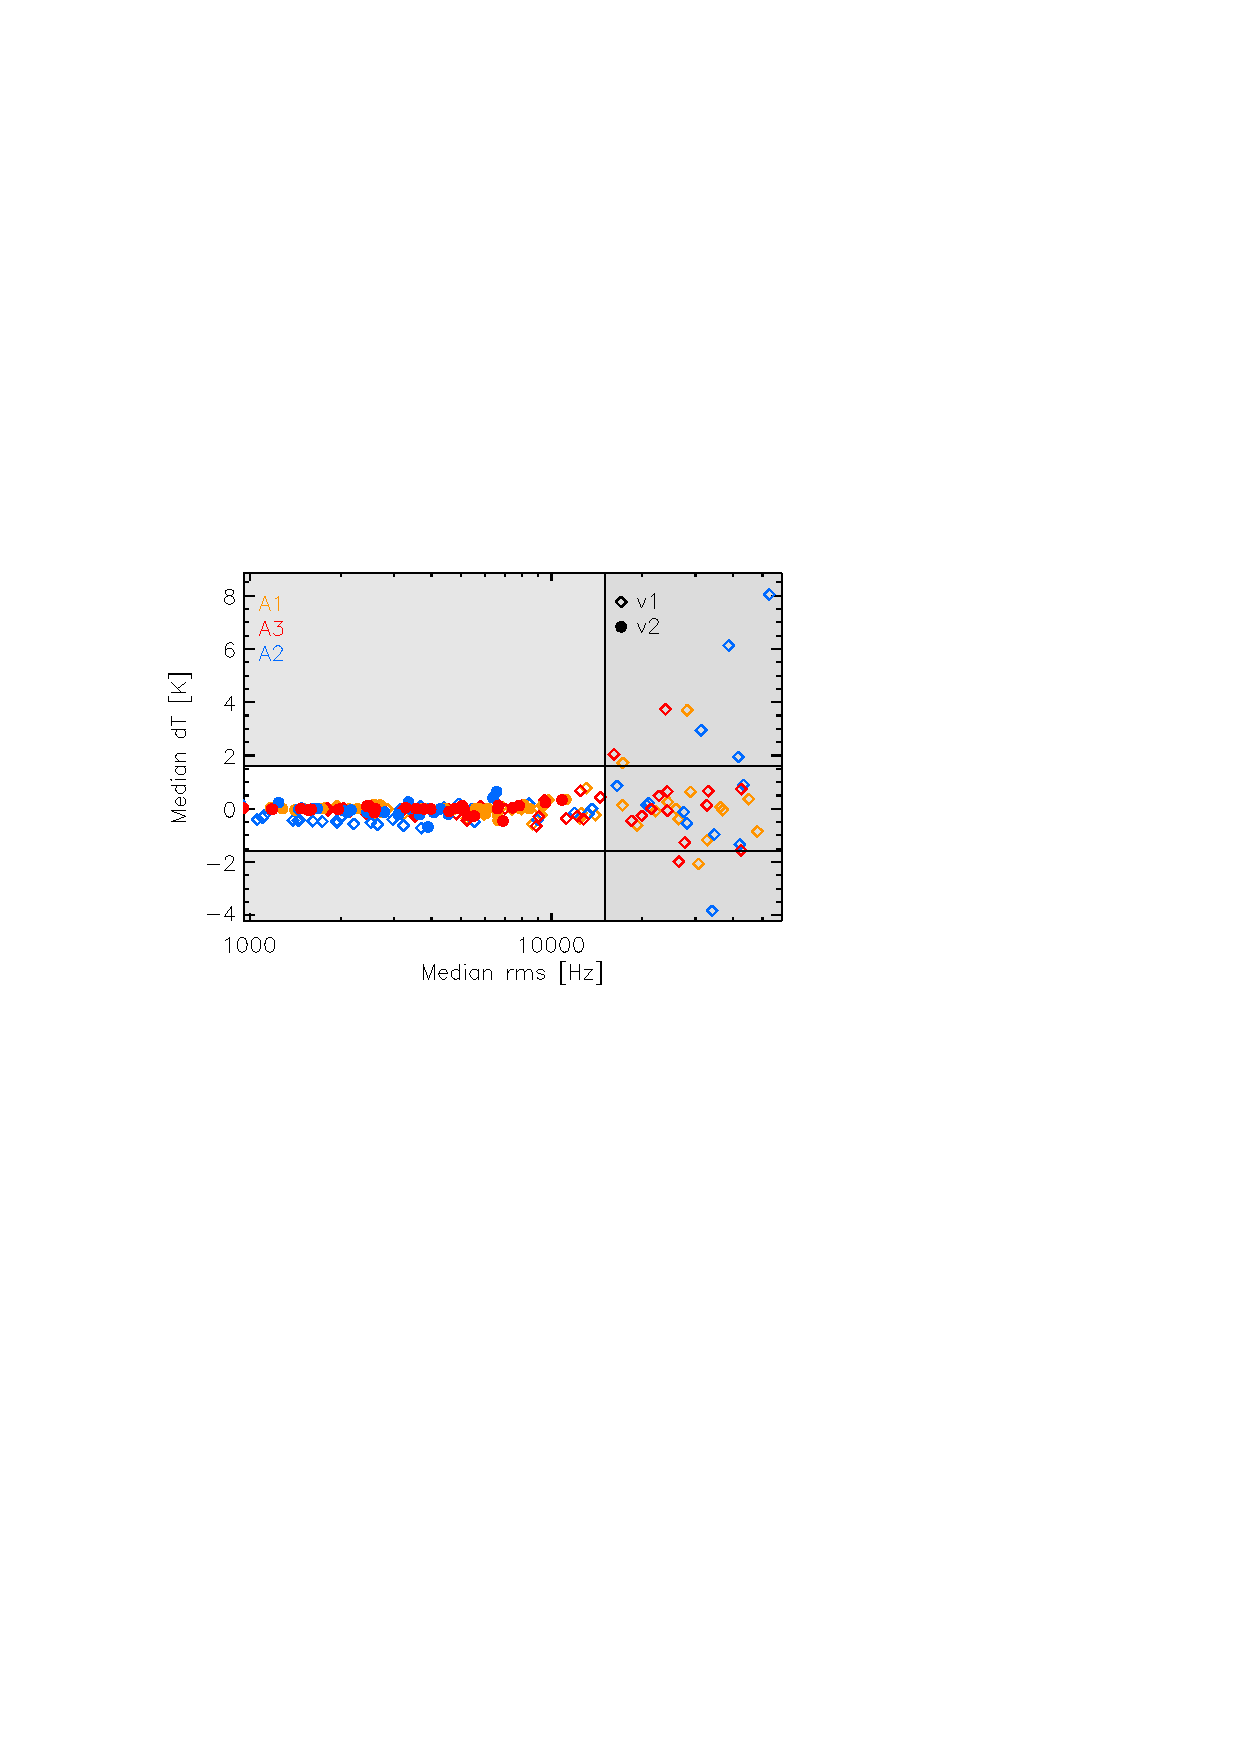
\includegraphics[clip=true,width=0.8\textwidth]{Figures/Opacity/plot_skydip_selection_two_crit.pdf}
\caption[N2R9 skydip scan selection.]{ Median dT quality-fit criterion is plotted in fonction of Median rms criterion for each skydip scans of the N2R9 campaign and for the three arrays. Both criteria are nicely correlated. Empty diamonds show the results of the first iteration of the skydip coefficient estimation, whereas filled circled show the second iteration, for which only the skydips that met both fit-quality criteria are included. After the second iteration, all the remaining skydips met the criteria.}
\label{fig:skydipselection}
\end{center}
\end{figure}

For each skydip scan and for each bunch of 40 KIDs, we compute the
difference between the measured KID resonance frequency and the model
given in Eq.~\ref{eq:skydip} taken at the best-fit values of the
($C_0$, $C_1$) parameters. Then we determine two indicators
of the fit quality per skydip. First, the standard deviation of the
measure-to-model difference is calculated over all the KIDs in a
bunch. For each skydip, we evaluate the median rms, which is the
median over the KID bunches of the standard deviation per bunch, given
in Hz. Secondly, for each scan, we compute the average
measure-to-model difference of each KID $k$, labelled $dT_k$, which is
then converted from Hertz to Kelvin using the $C_1$ parameter of the
KID $k$. Median $dT$ is the median of $dT_k$ over all the KID of an
array. With these two indicators in hands, we discard the skydip scans
that are noisy or that yield a poor fit by applying the selection
criteria

\begin{itemize}
\item Median $\rm{rms} < 1.5 \times 10^{4}~\rm{Hz}$
\item Median $dT < 1.6~\rm{K}$
\end{itemize}

The threshold values have been determined using the set of 44 skydip
scans of N2R9. The Median rms cut corresponds to twice the median of
this quantity per skydip scan, whereas the Median $dT$ cut is twice
the standard deviation of Median $dT$ over the skydips.
N2R9 skydip scan selection is illustrated in
Fig.~\ref{fig:skydipselection}, in
which the agreement between the two fit-quality criteria is clearly
seen. The ($C_0$, $C_1$) estimation proceeds in two steps: first the
parameters are estimated using all the available skydip scan for a
given campaign, then the estimation is re-iterated using the only
skydip scans that met the fit-quality criteria. After the second
iteration, we check that no extra skydip outlier are left, as shown by
the 'v2' label data points in Fig.~\ref{fig:skydipselection}. After
selection of the skydip scans acquired during the N2R9 campaign, 15
skydips are kept for the final step of the ($C_0$, $C_1$) fit. 


\begin{figure}[ht!]
  \begin{center}
    \includegraphics[clip=true, trim={0, -0.3cm, -0.3cm, 0},  width=0.42\textwidth]{Figures/Opacity/Skydip_selection_impact_a1.pdf}
    \includegraphics[clip=true, trim={0, -0.3cm, -0.3cm, 0},  width=0.42\textwidth]{Figures/Opacity/Skydip_selection_impact_a3.pdf}
    \includegraphics[clip=true, trim={0, -0.3cm, -0.3cm, 0},  width=0.42\textwidth]{Figures/Opacity/Skydip_selection_impact_1mm.pdf}
    \includegraphics[clip=true, trim={0, -0.3cm, -0.3cm, 0},  width=0.42\textwidth]{Figures/Opacity/Skydip_selection_impact_a2.pdf}
   \caption[Skydip selection impact on opacities]{Skydip-selection
    impact on the opacity estimates. For a series of calibration scans
    of MWC349 acquired during N2R9, the relative difference
    w.r.t. the baseline opacities $\tau_{\rm{base}}$ (labeled 'base')
    are shown as a function of $\tau_{\rm{base}}$ for five skydip
    selections. The most inclusive one (labeled 'incl')
    includes 38 skydips of the 44 available. 'night' comprizes 11
    skydips acquired during nighttime. 'low' consists of 20 skydips
    acquired in low opacity conditions. 'high
    1' and 'high 2' are fit-quality based selections relying of relaxed
    ('high1') or tighened ('high 2') criteria w.r.t. the baseline
    criteria given in Sect.~\ref{se:skydip-selection}. The dashed
    lines figure a $10\%$ opacity difference
    w.r.t. $\tau_{\rm{base}}$. } 
\label{fig:skydip-selection-impact}
\end{center}
\end{figure}


We test the stability of the ($C_0$, $C_1$) parameters against the
exact choice of the selection criteria.
We derive ($C_0$, $C_1$) parameter sets for the N2R9 campaign using
six skydip selections: the baseline selection (labeled 'base')
consists in the fit-quality based selection described above, which
comprizes 15 skydips, the selection labeled 'incl' consists of an
inclusive selection of 38 skydips in which only the noisier ones were
discarded, the 'night' selection comprizes 11 skydips acquired during
between 21:00 and 09:00 UT,
'high 1' and 'high 2' are two different selections, which comprize 23
and 13 skydips and are based on fit quality criteria that are
respectively relaxed or tighened with respect to the baseline criteria, 
and 'low' corresponds to a selection of 20 skydips acquired while
$\tau_{1mm} < 0.44$. Each ($C_0$, $C_1$) sets are used to derive
zenith opacity of the N2R9 calibration scans of MWC349. 
Figure~\ref{fig:skydip-selection-impact} shows the relative
difference between each $\tau$ estimates and the baseline $\tau$
estimates as a function of the baseline $\tau$. The relative
differences are basically constant for the whole opacity range: the
main effect of the skydip selection is a normalisation factor on the
$\tau$ estimates at both wavelength. At both wavelength, this factor
is below $10\%$ of the baseline $\tau$ for most of the skydip
selections. However, this is of about $10\%$ for the 'low' selection,
which highlight the necessity of including good skydips acquired in
high $(\tau_{1\rm{mm}} > 0.44)$ opacity conditions in the final
selection. The 'incl' (inclusive 38-skydip based) selection results in the larger
difference w.r.t. the baseline $\tau$, which are up to $20\%$ at 1mm
and up to $40\%$ at $2$mm, whereas the 'high 1' (mild quality-fit)
selection suffices to reduce the relative difference below $10\%$ at
1mm and below $15\%$ at 2mm.
As a summary, the $\tau$ estimates are robust against the exact skydip
selection as long as the selection includes good
skydips in high opacity condition $(\tau_{1\rm{mm}} > 0.44)$ and as the poor
fitting skydips are excluded. When these conditions are met, the
skydip selection induced uncertainties are below $10\%$ at 1mm and
below $15\%$ at 2mm. 

We conclude that opacities at both wavelengths can be reliably
estimated from a series of skydip scans using the (C0, C1) model.


%We conclude that opacities at 1mm can be reliably estimated from a series of skydip scans using the (C0, C1) model. %By contrast, for the 2mm opacities, a skydip-based method is not stable enough against the skydip selection. Thus, we adopt an hybrid approach. 

%\section{The hybrid method}

%The hybrid method comprizes two-steps: i) first the 1mm opacities,
%that are $\tau_{A1}$ and $\tau_{A3}$, are determined using the skydip
%method described in Sect.~\ref{se:skydip-method}, ii) then the 2mm
%opacity $\tau_{A2}$ is extrapolated from the 1mm ones using a modified
%ATM model. Namely, for the second step, we perform:

%\begin{equation}
%\tau_{A2} = \left( \left.\frac{\tau_{A2}^{\rm{ATM}}}{\tau_{A3}^{\rm{ATM}}}\right\vert_{\tau_{A3}} + \alpha \right) \tau_{A3},
%\end{equation}

% where $\alpha$ is an offset, which are estimated from the observations themselves, and the ratio is the predicted zenith opacity ratio for A2 and A3 frequency bands using the ATM model described in \ref{Pardo2002} and taken at the measured A3 zenith opacity. The zenith opacity expectations for the array $A_i$ is
%\begin{equation}
%  \tau^{\rm{ATM}}_{A_i} = - \ln{\frac{\int e^{-\tau^{ATM}(\nu)} T_{A_i}(\nu) d\nu}{ \int T_{A_i}(\nu) d\nu}},
%\end{equation}
%where the bandpasses $T_{A_i}$ for arrays $A_i$, $i=1, 2, 3$, are the Martin-Pupplet reference transmissions
%corrected by a Rayleigh-Jeans term  $T'_{A_i}(\nu) / \left( \frac{\nu}{\nu_0}\right)^2$. 

%We observe that the measured \emph{shape} of the measured opacity ratio is well described by the ATM expectations whereas its \emph{amplitude} is too low by an offset $\alpha$, which we dertermine using a data-driven approach. We estimate $\alpha$ as the offset that ensures a stability of the A2 flux over the whole opacity span.  

%\addparag{$\alpha$ fit + FIG}


%----------------------------------------------------------------------------------------
%	skydip opacity tests
%----------------------------------------------------------------------------------------
\section{Skydip-based opacity measurements and tests {\color{blue} Laurence}}
\label{se:skydip-opacity_tests}

We perform basic sanity tests of the skydip-based opacity
measurements, referred to as 'skydip' opacities hereafter.
First, we test the stability of the 'skydip' opacities from one
observation campaign to another.
Figure~\ref{fig:skydip-to-taumeter-correl} shows the
correlation between the 'skydip' $\tau$ estimates $\tau_{\rm{skydip}}$
and the taumeter zenith opacities $\tau_{225}$ for a series of scans
of Uranus and MWC349 acquired during three campaigns. As guidelines,
we also show the predicted correlations using an ATM model integrated
in NIKA2 wavebands. At 1~mm, the
$\tau_{\rm{skydip}}$ to $\tau_{225}$ correlation relations are
consistent for the three campaigns. They are
also in agreement with the ATM model expectations. At 2~mm, more
dispersion is observed between each correlation relations although
they are compatible with each others within statistical errors.
We note that the ATM model underestimates the
measured $\tau_{\rm{skydip}}$. This mild discrepancy with the
ATM model predictions is yet to be understood, but has no impact on
our opacity measurements, which do not rely on any ATM model nor on
the precision with which the observing bandpasses are known.


\begin{figure}[ht!]
  \begin{center}
    \includegraphics[clip=true, trim={0, -0.3cm, -0.3cm, 0}, width=0.42\textwidth]{Figures/Opacity/Opacity_correl_skydip_vs_tau_a1.pdf}
    \includegraphics[clip=true, trim={0, -0.3cm, -0.3cm, 0}, width=0.42\textwidth]{Figures/Opacity/Opacity_correl_skydip_vs_tau_a3.pdf}
    \includegraphics[clip=true, trim={0, -0.3cm, -0.3cm, 0}, width=0.42\textwidth]{Figures/Opacity/Opacity_correl_skydip_vs_tau_1mm.pdf}
    \includegraphics[clip=true, trim={0, -0.3cm, -0.3cm, 0}, width=0.42\textwidth]{Figures/Opacity/Opacity_correl_skydip_vs_tau_a2.pdf}
   \caption[NIKA2 skydip-based vs taumeter opacities]{ NIKA2
    skydip-based opacities vs IRAM 225GHz taumeter opacities. The
    modeled correlations relying on an ATM model integrated in NIKA2
    bands are shown in black.} 
\label{fig:skydip-to-taumeter-correl}
\end{center}
\end{figure}

We check the robustness of the 'skydip' $\tau$ againts the
observing elevation. 
Figure~\ref{fig:skydip-to-taumeter-ratio-vs-elev} shows the ratio of NIKA2
'skydip' opacities to the $225$GHz taumeter opacities as a function of
the observing elevation.

\begin{figure}[ht!]
  \begin{center}
    \includegraphics[clip=true, trim={0, -0.3cm, -0.3cm, 0}, width=0.42\textwidth]{Figures/Opacity/Opacity_skydip_to_taumeter_vs_elev_a1.pdf}
    \includegraphics[clip=true, trim={0, -0.3cm, -0.3cm, 0}, width=0.42\textwidth]{Figures/Opacity/Opacity_skydip_to_taumeter_vs_elev_a3.pdf}
    \includegraphics[clip=true, trim={0, -0.3cm, -0.3cm, 0}, width=0.42\textwidth]{Figures/Opacity/Opacity_skydip_to_taumeter_vs_elev_1mm.pdf}
    \includegraphics[clip=true, trim={0, -0.3cm, -0.3cm, 0}, width=0.42\textwidth]{Figures/Opacity/Opacity_skydip_to_taumeter_vs_elev_a2.pdf}
    \caption[NIKA2 skydip-based opacity stability against observing elevations]{NIKA2
    skydip-based opacities stability againts the observing elevation.} 
\label{fig:skydip-to-taumeter-ratio-vs-elev}
\end{center}
\end{figure}



%----------------------------------------------------------------------------------------
%	Corrected skydip method
%----------------------------------------------------------------------------------------
\section{Corrected skydip method {\color{blue} Laurence}}
\label{se:corrected-skydip}

%%%%%%%%%%%%%%%%%%%%%%%%%%%%%%%%%%%%%%%%%%%%%%%%%%%%%%%%%
% 1-params correction
%%%%%%%%%%%%%%%%%%%%%%%%%%%%%%%%%%%%%%%%%%%%%%%%%%%%%%%%%%
We use the flux stability estimators described in
Sect.~\ref{se:taumeter-method} to fit a correction to the 'skydip'
opacities $\tau_{\rm{skydip}}$ as
\begin{equation}  
  \tau_\nu =  a_\nu^{\rm{skydip}}\tau_{\rm{skydip}}.        
\end{equation}

We find $a_\nu^{\rm{skydip}}$ of
$1.36 \pm 0.04$,
$1.23 \pm 0.02$,
$1.27 \pm 0.03$ and
$1.03 \pm 0.03$ for A1, A3, A1$\&$A3 and A2 respectively.
% a   = 1.3600000       1.0318470       1.2326556       1.2660000
% s_a = 0.038587182     0.028553570     0.019324699     0.026832816


%%%%%%%%%%%%%%%%%%%%%%%%%%%%%%%%%%%%%%%%%%%%%%%%%%%%%%%%%
% 2-params correction
%%%%%%%%%%%%%%%%%%%%%%%%%%%%%%%%%%%%%%%%%%%%%%%%%%%%%%%%%%
\begin{figure}[ht!]
  \begin{center}
    \includegraphics[clip=true, trim={0, -0.3cm, -0.3cm, 0}, width=0.42\textwidth]{Figures/Opacity/fit_nika2_tau_from_skydip_mwc349_a1.pdf}
    \includegraphics[clip=true, trim={0, -0.3cm, -0.3cm, 0}, width=0.42\textwidth]{Figures/Opacity/fit_nika2_tau_from_skydip_mwc349_a3.pdf}
    \includegraphics[clip=true, trim={0, -0.3cm, -0.3cm, 0}, width=0.42\textwidth]{Figures/Opacity/fit_nika2_tau_from_skydip_mwc349_1mm.pdf}
    \includegraphics[clip=true, trim={0, -0.3cm, -0.3cm, 0}, width=0.42\textwidth]{Figures/Opacity/fit_nika2_tau_from_skydip_mwc349_a2.pdf}
    \caption[NIKA2 skydip-based opacity correcting
    relation]{Fit of the skydip-based opacity correcting relation
    parameters.
    The flux-stability estimator contours are shown in the plan
    $a_{\rm{skydip}} \equiv a_\nu^{\rm{skydip}'}$ and
    $b_{\rm{skydip}} \equiv b_\nu^{\rm{skydip}'}$
    for A1, A3, A1$\&$A3 and A2.
    The red contours enclose rms
    errors of the measured-to-median flux density ratio of $5.5$, $7$
    and $10\%$ at 1mm and $2.7$, $3.5$ and $5\%$ at 2mm. The blue
    contours correspond roughthly to the $68\%$, $95\%$ and $99\%$
    confidence levels drawn from the $\chi^2$ estimates.
    The best fit values are shows as green stars. Offset
    $b_\nu^{\rm{skydip}'}$ are compatible with zero within the $68\%$
    CL contours.} 
\label{fig:skydip_fit}
\end{center}
\end{figure}

Moreover, we test for an offset $b_\nu^{\rm{skydip}'}$ in the
correcting relation of the 'skydip' opacities as 
\begin{equation}  
  \tau_\nu =  a_\nu^{\rm{skydip}'}\tau_{\rm{skydip}} + b_\nu^{\rm{skydip}'}.      
\end{equation}
We repeat estimating the parameters of the correcting
relation. Confidence level contours in the parameter plan using the
two stability estimators are skown in Fig.~\ref{fig:skydip_fit}, as
well as the
best-fitting parameter values.
We find the best-fit $a_\nu^{\rm{skydip}'}$ estimates of
$1.36 \pm 0.04$,
$1.25 \pm 0.07$,
$1.28 \pm 0.04$ and
$1.05 \pm 0.05$ for A1, A3, A1$\&$A3 and A2 respectively, which are in
agreement with the best-fit values estimated using the single-parameter
correcting relation, whereas the best-fit values of the offsets
$b_\nu^{\rm{skydip}'}$ are compatible with zero at both wavelengths.
% a   = 1.3600000       1.0467126       1.2476650       1.2792013
% s_a = 0.037853031     0.050552977     0.068354972     0.044088207
% b   = -0.0053333333    -0.014432990    -0.040000000    -0.030731707
% s_b = 0.011925696     0.012184154     0.030641294     0.020823168


  % Xavier&Laurence
%----------------------------------------------------------------------------------------
%	OPACITY MEASURES
%----------------------------------------------------------------------------------------

\section{Opacity measurements {\color{blue} Juan $\&$ Laurence}}
\label{se:opacity_correction}

%{\bf copy from the 'Instru' paper}

%\begin{figure}[ht]
%\begin{center}
%\includegraphics[scale=0.8]{Figures/test_allskd_N2R10v3commiss2.pdf}
%\caption{Atmospheric opacity as measured from the NIKA2 data 
%at 260 (top) and 150\,GHz (bottom) during N2R10
%commissioning campaign. Each block of 40 KIDs gives an independent estimate of
%the opacity value for each skydip scan (the integer abscissae). The block
%number is the decimal value of the abscissae.
%\label{fig:taumeas_paper}}
%\end{center}
%\end{figure}

%\begin{figure}[ht]
%\begin{center}
%\includegraphics[scale=0.8]{Figures/test_allskd_N2R10v2commiss1.pdf}
%\caption{Atmospheric opacity as measured from the NIKA2 data 
%at 260 and 150\,GHz during N2R10
%commissioning campaign. The error bars are in fact dispersion of the deduced
%opacities between blocks of 40 KIDs.
%\label{fig:taumeas_paper}}
%\end{center}
%\end{figure}

We observe that the skydip-fitted $\tau$ values are, as expected, common
between different detectors of the same array. By comparing the results of different skydips, we
have verified experimentally that the coefficients $C_0$, $C_1$ are stable,
within the fit errors, on very long time scales within a cooldown cycle. The
coefficients can thus be applied to the whole observing campaign in order to
recover the opacity of each scan.


% \noindent {\bf FM : a figure would help to convince the reader that it is stable on lng time
% scale, which is a key point.}\\ FXD: I will do that figure


\begin{figure}[ht]
\begin{center}
\includegraphics[scale=0.8]{../../../Paper_NIKA2_Technical/opacity_evol_run22.pdf}
\caption[Zenith opacity monitoring during N2R9]{Atmospheric opacity as measured from the IRAM 225\,GHz taumeter
(cyan), and from the NIKA2 data at 150 (red) and 260\,GHz (blue) during N2R9
commissioning campaign (Feb. 2017). We stress the fact that the IRAM 225\,GHz
taumeter data is not used for the atmospheric correction and is plotted here
just for comparison.
  \label{fig:taumeas_paper}}
\end{center}
\end{figure}


\begin{figure}[ht]
\begin{center}
\includegraphics[width=\linewidth]{Figures/opacity_vs_index_N2R9_N2R10.png}
\caption[Zenith opacity monitoring during N2R9 and N2R10]{Atmospheric opacity as measured from the IRAM 225\,GHz
  taumeter (black crosses), and from the NIKA2 data at 150 (red) and 260\,GHz (blue) during 
  N2R9 and N2R10 commissioning campaigns.  We stress the fact that the IRAM 225\,GHz taumeter data is not used for the atmospheric correction and is plotted here just for comparison.
  \label{fig:taumeas}}
\end{center}
\end{figure}


In Fig.~\ref{fig:taumeas} {\bf(and Fig.~\ref{fig:taumeas_paper} of
  \cite{Adam18}) } we present the evolution of the NIKA2 in-band
opacities for all the 'OTF' scans (about 1300 scans per runs) of the
N2R9 run held in February and the N2R10 run in April 2017. These are
compared to the IRAM tau-meter values. We observe an agreement on the global trend between the IRAM tau-meter opacity (225 GHz) and the NIKA2 values. These latter show, however,
a smaller dispersion (less than one percent).


 % Juan&Laurence


\clearpage
%----------------------------------------------------------------------------------------
%	FOCAL PLANE RECONSTRUCTION
%----------------------------------------------------------------------------------------
\chapter{Focal Plane Reconstruction {\color{blue} Nico et al.}}
\label{se:fp_reconstruction}
%----------------------------------------------------------------------------------------
%	FOCAL PLANE RECONSTRUCTION
%----------------------------------------------------------------------------------------
%\section{Focal Plane Geometry}
%\label{se:geometry}


%   Methods
%----------------------------------------------------------------------------------------
\subsection{FOV position reconstruction}
\label{se:fov_geometry}

In order to be able to produce a map, one needs to associate a pointing
direction to any data sample of the system. The telescope provides us with
various pointing information for a reference position in the focal plane. We
then need to know the relative pointing offsets of each detector. We use
\bms\ for this purpose (see Sect.~\ref{se:beammaps}). The determination of the
KID offsets in the focal plane proceeds in two steps.

\paragraph{Step 1.} We apply a median filter per
KID timeline whose width is of 31 samples, that is equivalent to about 
5~FWHM at 65 arcsec/s given that the sampling frequency is 23.84~Hz,
and we project one map per KID in Nasmyth
coordinates. This median filter removes
efficiently most of the low frequency atmospheric and electronic
noise, albeit with a slight ringing and flux loss on the
source. However, at this stage, we are only interested in the location
of the observed planet.
To derive the Nasmyth coordinates from the
provided $(\alpha_t,\delta_t)$ and $(\Delta\alpha_t,\Delta\delta_t)$
coordinates, we build the following quantities at time~$t$:

\begin{eqnarray}
\Delta x_t &=& \cos\delta_t \Delta\alpha_t - \sin \delta_t\Delta \delta_t \nonumber \\
\Delta y_t &=& \sin\delta_t \Delta\alpha_t + \cos \delta_t\Delta \delta_t \nonumber
\end{eqnarray}

Note that $\Delta\alpha_t$ is already corrected by the $\cos\delta_t$ factor to
have orthonormal coordinates in the tangent plane of the sky and be immune to
the geodesic convergence at the poles. Moreover, before projecting the
time-ordered data onto maps, we check
the accuracy of the time-stamping and the consistency between the
telescope time and NIKA2 time. First, we test the
synchronisation of the electronic boxes and the regularity of the
time increase. In case of detection of an anomaly, the
time-stamping of the impacted data samples is
recalculated by interpolating from the accurately stamped
neighbour samples. Then, a so-called \emph{zigzag}
procedure is used to test for delay between the telescope pointing
information and NIKA2 timelines: we fit a constant shift between the
source positions estimated using the subscans in one direction and
using the subscans in the opposite direction. The data timelines are
then projected onto maps. 
We fit a 2D elliptical Gaussian on
each KID map. The centroid of this Gaussian is a first estimate of the KID
offsets, FWHM's, ellipticity and sensitivity. We apply a first KID selection by
removing outliers to the statistics on these parameters. We also discard
manually KIDs that show a cross-talk counterpart on their map.

\paragraph{Step 2.} With these offsets, it is already possible to produce maps
from the combination of all detectors. However, in order to go up to
the calibration stage, we must correct for the flux loss induced by
the median filter and ensure that each timeline is treated in the same
way as the final observation will. For this, we apply the pointing
reconstruction presented in Sect.~\ref{se:ptg} and the data reduction
presented in Sect.~\ref{se:toi_proc}. We still do not have absolute
calibration for each KID (no opacity correction yet) but the amplitude
of the fitted centroid on the same planet provides the required
cross-calibration between KIDs. The final absolute calibration will be
presented in Sect.~\ref{se:calibration}.\\

This analysis is repeated on all \bms\ to obtain statistics and
precision on each KID parameter, together with estimates on KID
performance stability, as discussed in the next sections.

\subsection{FOV grid distortion}
\label{se:grid_distortion}

We studied the matching of the KID position on the sky to the
design position. The global result is scaling, rotation, and shift
parameters for each array. They are described in Table~\ref{ta:gridmatch}.

\begin{table}[ht]
\label{ta:gridmatch}
\begin{center}
\begin{tabular}{|c|c|c|l|}
\hline
Array 1  &	Array 3   &	Array 2   &	Comment \\
\hline
1.25     &      1.25      &     2.05     &     \small{$\lambda$ in mm} \\
1140 	 &      1140 	   &        616  &     \small{Total of designed KIDs (TDK)} \\
673/736  &	734/758  &	437/444  &     \small{Well-placed KIDs (WPK)/Found KIDs (FK)} \\
91/59 	 &    96/64 	 &      98/71 	 & \small{Ratio [\%] of WPK/FK and WPK/TDK} \\
0.87 	 &     0.84 	  & 0.66     &	\small{Median deviation [arcsec] for detectors deviating by less than 5~arcsec} \\
0.52 	 &     0.69 	 &        0.68 	 & \small{Mean distortion across the FoV in arcsec} \\
2.3 -4.5  &	2.0 -5.8  &	9.3 -7.5  &	\small{Array center in Nasmyth coordinates [arcsec]} \\
4.90  &	4.88  &	4.88  &	\small{Plate scaling [arcsec/mm] in the Design x and y (averaged)} \\
77.3  &	76.4  &	78.2  &	\small{Plate rotation angle [degree] from the Design to Nasmyth coordinates} \\
6.6  &	6.6  &	6.6  &	\small{FOV [arcmin] (Total KIDs)} \\
9.8/2.00  &	9.7/2.00  &	13.3/2.75  &	\small{Distance between near detectors [arcsec, mm]} \\
% Old values, rechecked (difference comes from lambda and D)
%   1.24  &	1.22  &	0.97  &	Distance between near detectors with $30\,\rm{m}$ diameter aperture [in $\lambda$/D] \\
% here new values checked FXD 30 Nov 2018:
1.11  &	1.10  &	0.87  &	\small{Measured Distance between near
  detectors [in $\lambda$/D] } \\
%\new{with $27\,\rm{m}$ effective diameter aperture} [in $\lambda$/D]} \\
1.09  & 1.09  & 0.93  & \small{Modeled Distance with ZEMAX}\\
\hline
\end{tabular}
\end{center}
\caption[Field-of-view deformations]{Linear 2D fit of the observed
  position of the detectors in the sky for N2R9 against their mechanically
  designed position. The initial table of Found KIDs is given
  by the focal plane geometry procedure, as described in
  Sect.~\ref{se:fov_geometry},
  applied to N2R9 \bm\ scans. More than 90\% of the detectors (WPK/FK) are
  within less than 5 arcseconds of their expected position. }
\end{table}

It shows that on average the position of each detector is known to better than
an arcsecond. The 1\,mm arrays have almost the same center but this center
differs by 7 and 2\,arcsec in Nasmyth coordinates from the
2\,mm array center. The sampling is above
$\lambda/D$ at 1\,mm, assuming a 27\,m effective diameter aperture. Note that
the plate rotation angle was designed as 76.2\,degrees, less than 2
degrees from what is observed. We find that array 1
has some of the most deviant detectors (above 4\,arcsec from their expected
position). These detectors should be excluded from further analysis. We call
distortion (in the table) the $x.y$ term in the polynomial fitting between the
design grid and the observed position (the fitting is done with the $x$ and
$y$ linear terms and the $x.y$ term). 

This has been compared to expectations obtained using ZEMAX
simulation. 
%The grid diagram generated using ZEMAX provides us with
%the maximum dispersion in the field defined by
%
%\begin{equation}
%P = \frac{\sqrt{(x_p - x_r)^2 + (y_p - y_r)^2}}{\sqrt{x_p^2 + y_p^2}},
%\end{equation}
%
%where $(x_p, y_p)$ and $(x_r, y_r)$ are respectivelly the predicted
%and real coordinates on the image surface relative to the reference
%field position image location (see page 170 of the ZEMAX manual, 2007).
%The predicted coordinates for the whole field are obtained using a
%linear interpolation of a small area in the field central part,
%whereas the real coordinates are calculated by ray tracing through the
%optical system.
%
%\begin{figure}[ht] 
%\begin{center}
%  \includegraphics[width=0.9\textwidth]{Figures/NIKA2_Grid-distortion.png}
%  \caption[Simulated FOV grid]{NIKA2 grid diagram simulated using
%    ZEMAX. \new{The step of the grid is of 30 arcsec and the side width
%      of the black square is of seven arcmin. The red circle corresponds to the 
%      $6.5\,\rm{arcmin}$ diameter FOV. Blue crosses show the grid
%      distorsions in az-el coordinates and in the case of an observing
%      elevation of $14^o$. These grid distorsions depends on the
%      telescope elevation, whereas in the image plane (the plane of the
%      KID arrays) the distorsions are invariant. This allows for
%      concluding that the grid distorsions are caused by the optical
%      elements located between M4 and the dichroic plate.} 
%  }
% \label{fig:fov_grid_distortion_zemax}
%\end{center}
%\end{figure}
%Figure \ref{fig:fov_grid_distortion_zemax} shows the ZEMAX grid diagram for
%NIKA2 simulated optic system.
%
We generated a grid diagram for NIKA2 optic system and found a maximum
grid distortion of $2.7\%$ in the $6.5'$ FOV. We notice that the
strongest distortion appear in the upper right corner of the Nasmyth plan, which is
also the area of the largest defocus w.r.t. to the center (see
Sect.~\ref{sec:focus_surfaces}).
An expected distortion of $2.7\%$ is at most a 5'' shift from the
center to the outside of the array. The quoted distortions between the
measured and designed positions are consistent with the expected
maximum distortions from the NIKA2 optics.

%Auxillary information on this work can be found in this wiki post\footnote{\tiny
%  {\tt http$://$www.iram.fr$/$wiki$/$nika2$/$index.php$/$April$\_$19,$\_$2017,$\_$FXD,$\_$KID$\_$position$\_$mapping$\_$and$\_$Field$\_$distortion$\_$for$\_$Run9}}.
% FXD: this would need to be more ascertained. Lack of time to go further.


\subsection{KID selection and average geometry}
\label{avg_kidpar}

\begin{figure*}[!tp]
\begin{center}
\includegraphics[trim=2cm 14cm 4cm 4cm, clip=true,width=0.45\linewidth]{Figures/A1_fwhm_color_count.pdf}
%\includegraphics[trim=2cm 14cm 5cm 4cm, clip=true,width=0.45\linewidth]{Figures/A1_positions.pdf}
\includegraphics[trim=2cm 14cm 4cm 4cm, clip=true,width=0.45\linewidth]{Figures/A3_fwhm_color_count.pdf}
%\includegraphics[trim=2cm 14cm 5cm 4cm, clip=true,width=0.45\linewidth]{Figures/A3_positions.pdf}
\includegraphics[trim=2cm 14cm 4cm 4cm, clip=true,width=0.45\linewidth]{Figures/A2_fwhm_color_count.pdf}
%\includegraphics[trim=2cm 14cm 5cm 4cm, clip=true,width=0.45\linewidth]{Figures/A2_positions.pdf}
\caption[KID selection in the FOV]{Average detector positions
  for arrays A1, A3, and A2. The three plots show the detectors that have seen
  the sky and passed the quality criteria for at least two \bms\ during Run10, 9
  and 8: 952, 961, and 553 for A1, A3 and A2, respectively. The color
  indicates, from green to red, how many times a KID was
  identified as valid on a \bm. The inner and outer
  dash-line circles correspond to a FOV of 5.5\,arcmin and 6.5\,arcmin,
  respectively. Units are arcseconds.}
\label{fig:avg_fov_color}
\end{center}
\end{figure}

In order to identify the most stable KIDs, we compare the KID parameters
obtained with several \bms.  In the following, we show results as obtained using
seven \bms\ from Run10, two from Run9 and one from Run8.  For each KID we
compute the average position on the focal plane and the average FWHM, counting
the times that it has been considered as valid and at the same position. Indeed,
a few KIDs have close resonances and can be tuned and switched on some scans. A
few others must also be discarded because they appear identical numerically due
to \samu{the fact that a same (noisy) KID can sometimes be associated
  to two different frequency tone in the acquisition.}
%a remaining artefact in the acquisition.
These KIDs are flagged out (less than 1\% of the designed KIDs).

In Fig.~\ref{fig:avg_fov_color} we show the
average focal plane reconstruction, from green to red depending on the number of
times that the KID has been considered as valid.
\new{The eight internal readout feed lines that connect each of the two
  $1\,\rm{mm}$ arrays are also noticeable in this figure: first, slightly
  larger spaces are seen between KID rows connected to different
  feed-lines than between KID rows of the same feed line and second, KIDs at the end of a
  feed line are less often valid than others (see e.g. the FOV of
  Array 3). For A1, this end-of-feedline effect is mixed with the
  effect of the KID gain variation across the FOV, which mainly affects
  the South-West third of the array, as discussed in Sect.~\ref{se:flatfields}.}

For A1, A3 and A2, respectively, we have 952, 961, and 553 KIDs that
have been considered as valid at least twice (840, 508, 868 valid at
least five times). Using this criterion, we deduce the fraction of
valid detectors over the designed ones, as given in Table~\ref{tab:number_of_kids}.

%% \begin{figure}[htp]
%% \begin{center}
%% \includegraphics[trim=2cm 14cm 5cm 4cm, clip=true,width=0.55\linewidth]{Figures/A1_positions.pdf}
%% \includegraphics[trim=2cm 14cm 5cm 4cm, clip=true,width=0.55\linewidth]{Figures/A3_positions.pdf}
%% \includegraphics[trim=2cm 14cm 5cm 4cm, clip=true,width=0.55\linewidth]{Figures/A2_positions.pdf}
%% \caption[Stability of KID positions in the field-of-view]{For the valid
%%   detectors, we show the positions of each pixel, as obtained from each beam
%%   map. Some of them are not found at the same position for all the \bms.
%% Units are arcseconds. \todo{{\bf FM : color code : same as on the 1st
%%       maps of validity}}}
%% \label{fig:jumping_kids}
%% \end{center}
%% \end{figure}

%\begin{figure}[htp]
%\begin{center}
%\includegraphics[trim=2cm 14cm 5cm 4cm, clip=true,width=0.55\linewidth]{Figures/A1_test_positions.pdf}
%\includegraphics[trim=2cm 14cm 5cm 4cm, clip=true,width=0.55\linewidth]{Figures/A3_test_positions.pdf}
%\includegraphics[trim=2cm 14cm 5cm 4cm, clip=true,width=0.55\linewidth]{Figures/A2_test_positions.pdf}
%\caption[Average KID positions]{For the valid detectors,
%  we show the mean (red crosses) and the median (black squares)
%  positions of each pixel, as obtained from each \bm.
%  Units are arcseconds. \todo{FM : color code ? same as on the 1st maps of validity}}
%\label{fig:mean_vs_median}
%\end{center}
%\end{figure}

\begin{table}[ht]
\begin{center}  
  \begin{tabular}{|c|c|c|c|}
    \hline
    Array & Designed detectors &  Valid detectors & Fraction\\
    \hline\hline
    A1 & 1140 & 952 &  84\%\\
    A3 & 1140 & 961 &  84\%\\
    A2 & 616  & 553 &  90\%\\
    \hline
  \end{tabular}
  \caption[Number of detectors]{Summary of the number of valid detectors per array.}
  \label{tab:number_of_kids}
\end{center}    
\end{table}


% + Focal Plane Geometry
% + KID selection and average geometry
% + FOV grid distortion
% + Reconstruction of the focus surfaces


\clearpage
%----------------------------------------------------------------------------------------
%	BEAM PATTERN
%----------------------------------------------------------------------------------------
\chapter{Beam pattern {\color{blue} Laurence et al.} }
\label{se:beams}
% Full Beam Pattern + beam variations
%%
%%
%%      SECTION: BEAM PATTERN 
%%

%% [intro]
%%________________________________________________________

The NIKA2 beam pattern mainly depends on the IRAM 30m telescope and
NIKA2 full (external and internal) optical system characteristics,
whereas the detectors themselve might have an impact at sub-dominant
level (through e.g. time constants or correlated noises).

In this section, we characterize both the main beam, which is
modeled as an elliptical Gaussian, and the full beam pattern including
error beams up to angular scales of 10 arcmin.

%% [Full beam pattern]
%%________________________________________________________
\section{Full beam pattern {\color{YellowGreen} Laurence}}
\label{se:fullbeam}

\subsection{Data sets}
\label{se:beammap_set}

The characterization of the IRAM $30\,\rm{m}$ beam pattern observed
through NIKA2 detectors is mainly based on observations of strong
compact sources, such as planets including Uranus, Neptune and Mars,
and bright quasars. We generally use \bm\ scans, which are described
in Sect.~\ref{se:beammaps}.
Most of our beam-related analysis are based on a
set of 18 \bm\ scans acquired during the N2R8 and N2R9 commissioning
campaigns and the N2R12 and N2R14 science pools. Namely, the set
consists of the N2R8 '20170125s243' scan, the N2R9 '20170224s177',
'20170226s415', '20170226s425' and '20170227s84' scans, the N2R12
'20171022s158', '20171023s101', '20171024s105', '20171024s106',
'20171025s41', '20171025s42',  '20171027s49',  '20171028s310',
'20171029s266', '20171030s268' and  '20180117s92' and the N2R14
'20180117s92',  '20180122s82' and  '20180122s309' scans.

This set of \bm\ have been selected from all the available \bm\ at
optimal focus using the baseline selection criteria, as given in
Sect.~\ref{se:data_selection}.



\subsection{Deep beam maps}
\label{se:deep_beam_maps}
We present the two-dimensional distribution of the beam in
Fig.~\ref{fig:beam}. We primary use a map obtained from a combination
of deep observations of strong point sources collected during
\emph{NIKA2-run8} and \emph{run9}. Namely, we use 'beammap' OTF scans
of Uranus (scan id '20170125s223' and '20170125s243'),  Neptune
('20170224s177') and the bright quasar 3C84 ('20170226s415'). However,
we checked the stability of our results on single scan maps,
combinations of scans for a single source, and combinations of
shallower scans but spanning a large range of scanning direction. The
data processing includes a mitigation of the correlated noise, which
mainly originates from the atmosphere.  We primarly use a subtraction
of a common mode estimated from the most correlated detectors (the
so-called 'cm one block' method). However, other methods are tested
for assessing the immunity of our results to noise residuals.

\begin{figure}[ht!]
\begin{center}
  \includegraphics[clip, angle=0, scale=0.4]{Figures/Lobe_map_Combo_v2_dB.pdf}
 \caption[Beam pattern.]{From upper left to lower right, beam maps of array 1 (labeled 'A1'), array 3 ('A3'), the combination of the 1.15mm arrays ('A1$\&$3') and the 2mm array ('A2') are shown in decibel. These maps, which consist of normalized combination of four long OTF scans of bright point sources, are in celestial coordinates and cover a sky area which extend over 10 arcmin.}
\label{fig:beam}
\end{center}
\end{figure}

The deep NIKA2 beam maps reveal some noticeable features, which are
shown in Fig.~\ref{fig:features} and which comprize:
\begin{itemize}
\item[(1)] four symmetrical spokes of the error beam as shown by
  yellow arrows in the A2 panel, which are expected from \emph{Zemax}
  simulations;
\item[(2)] shallow spikes of unknown origin, which are circled by pink
  ellipses. The multiple images on the combined deep beam map indicate
  a rotation of these spikes with the observing elevation, which in
  turn point to diffraction related issue or a ghost image that are
  formed inside the cryostat;
\item[(3)] other spikes of unknown origin, as pointed with the yellow
  arrows in the A3 panel. The ones that are close to the vertical and
  horizontal radii are reproduced by 'Zemax' simulation but with a  
  shallower, whereas the ones in the diagonal directions may be due to
  external calibrator installed close to the secondary mirror.  
\end{itemize}

\begin{figure}[ht!]
\begin{center}
  \includegraphics[clip, angle=0, scale=0.4]{Figures/Beams_features.pdf}
\caption[Noticeable features of NIKA2 beam pattern.]{ Red circle: diffraction ring seen in 1-mm maps (the spokes are presumably caused by radial and azimuthal panel buckling (cf. Fig.4 in Greve et al. 2010)); Perpendicular green lines: diffraction pattern caused by quadrupod secondary support structure (prominently seen in 2mm maps); Yellow arrows in the upper right pannel: pattern of 3 spikes seen in 1mm maps of unknown origin; Yellow arrows in the lower right pannel: four symmetrical spokes of the first errorbeam; Pink ellipses: 4 spikes seen in 2mm maps.}
\label{fig:features}
\end{center}
\end{figure}


To gain a first impression of the structure of the Iram 30-m beam as
seen with NIKA2, we use radial cuts to evidence the relative level of
the main beam, the first error beam and other features seen in the 2D
beam pattern using radial cuts. NIKA2 full beam is shown in the left
panels of Fig.~\ref{fig:beam_structure_example} by means of two
orthogonal cuts through Uranus from a high quality map obtained on
2017 January 25th in excellent observing conditions
(low opacity $\tau_{225}=0.08$ and elevation $46^{\circ}$).


\begin{figure}[ht!]
  \begin{center}
    \includegraphics[clip=true, width=0.39\textwidth]{Figures/Array_A1_dB.pdf}
    \includegraphics[clip=true, trim={-0.5cm, -0.65cm, 0, 0}, width=0.44\textwidth]{Figures/Beam_profiles_A1_FR.pdf}
    \includegraphics[clip=true, width=0.39\textwidth]{Figures/Array_A3_dB.pdf}
    \includegraphics[clip=true, trim={-0.5cm, -0.65cm, 0, 0}, width=0.44\textwidth]{Figures/Beam_profiles_A3_FR.pdf}
    \includegraphics[clip=true, width=0.39\textwidth]{Figures/Array_A2_dB.pdf}
    \includegraphics[clip=true, trim={-0.5cm, -0.65cm, 0, 0}, width=0.44\textwidth]{Figures/Beam_profiles_A2_FR.pdf}
    \caption[Beam structure]{\emph{Left column:} Two orthogonal cuts through the
      beam are shown in red and green and a best fit model made of three
      Gaussians is superimposed in black.
      These cuts were obtained from the high quality map of Uranus on 2017
      January 25th. The main beam starts to depart from the first Gaussian
      at -12dB. \emph{Right column:} Example of beam radial profile
      estimated on the same map of Uranus. The Best-fitting curve is show
      in red using a three Gaussian model.   
    }
    \label{fig:beam_structure_example}
    %\label{fig:beam_profiles_3G}
  \end{center}
\end{figure}

A model made of three Gaussians centered on the source peak was best
fit {\it by hand} to these cuts.
%the parameters are reported in Table \ref{tab:3gauss} [PEUT-ETRE
%AVANTAGEUSEMENT REPLACED PAR VALEURS DE FLORIAN].
We observe that the main beam starts to depart from the first
Gaussian at the level of about -12dB for the three arrays.
We note that for the instrument EMIR on the radiotelescope,
this departure is about -20dB (Kramer, Penalver and Greve
2013). However, this
discrepancy between a feedhorn-based experiment and a bare pixels one
is expected since the main effect of the feedhorns is to lower the
side lobes of the Airy diffraction pattern.
The precise characterization of the full beam structure is discussed
in Sect.~\ref{se:fullbeam_prof}.  

%From parameters in Table \ref{tab:3gauss}, one can estimate that
%the source incident power is split about equally between the main beam
%and the error beam at 1mm, and these fractions are 70\% and 30\% at 2mm, respectively.
%This modelling uses the central
%region   $180'' \times 180''$ in size with a uniform noise rms from
%a larger area of 8' x 5' on the sky scanned with the arrays. It is expected
%that the error beam extend beyond these limits.


%\begin{table}
%\centering 
%\caption[]{Model parameters of the three Gaussian beam.}
%\begin{tabular}{|l|l|l|l|l|l|l|}
%\hline
%               & \multicolumn{3}{c|}{A1 and A3} & \multicolumn{3}{c|}{A2}  \\
%\hline
%fwhm      & $11.25''$ & $45''$  & $250''$ & $17.75''$ & $56''$  & $420''$ \\
%amplitude & 0.984     & 0.015   & 0.0005   &  0.9875   & 0.011   &  0.0005\\
%\hline
%\end{tabular}
%\label{tab:3gauss}
%\end{table}


\subsection{Beam profile}
\label{se:fullbeam_prof}

The beam profile $B(r)$ is the radial brightness profile normalized so
that $B(0) = 1$, where $r$ is the radius from the beam center.
%is the azimuthal average of the beam map around the
%main beam center.
Although the profile cannot represent the sub-dominant non-axisymetrical
extended features, which are seen in the beam pattern and discussed in
Sect.~\ref{se:deep_beam_maps} (telescope arms, spikes), it provides us with a useful
representation of the internal and central parts of the beam (about up to
$100''$). We determine a beam profile from a beam map in centering to
the fitted value of the main beam center and in forming the
weighted average of the pixels equidistant to the center.

We model the beam profile $B(r)$ as a three-Gaussian function defined as:
\begin{equation}
  B(r) = \sum_i \mathcal{A}_i G_i(r) + \mathcal{B}_0,
  \label{eq:3gauss}
\end{equation}

where $\mathcal{A}_i$ the amplitude of the Gaussian $i$ for $i \in {1, 2, 3}$ and
$\mathcal{B}_0$ a piedestal level accounting for the residual noise
level in the map.
An example of the beam profile from a beam map acquired during {\emph N2R8} (scan ID:
20170125s223), as well as the best-fit 3-Gaussian model, is shown in
the right panels of Fig.~\ref{fig:beam_structure_example}.


%%%%%%%%%%%%%%%%%%%%%%%%%%%%%%%%%%%%%%%%%%%%%%%%%%%%%%%%%%%%%%%%%
% Stability of the beam pattern
We checked the stability of the beam against various observing
conditions (source intensity, weather condition, focus optimisation) by
comparing the beam profiles of the \bm\ set, as described in
Sect.~\ref{se:beammap_set}. The 18 beam profiles and their difference
w.r.t. the median beam profile are shown in Fig.~\ref{fig:beam_prof}.
The variations of the normalised radial profiles are below $5\%$ at
both wavelengths. 


\begin{figure}[ht!]
  \centering
   \includegraphics[clip, width=0.42\textwidth]{Figures/Beams/plot_profiles_a1.pdf}
   \includegraphics[clip, width=0.42\textwidth]{Figures/Beams/plot_profile_diff_wrt_median_a1.pdf}
   \includegraphics[clip, width=0.42\textwidth]{Figures/Beams/plot_profiles_a3.pdf}
   \includegraphics[clip, width=0.42\textwidth]{Figures/Beams/plot_profile_diff_wrt_median_a3.pdf}
   \includegraphics[clip, width=0.42\textwidth]{Figures/Beams/plot_profiles_1mm.pdf}
   \includegraphics[clip, width=0.42\textwidth]{Figures/Beams/plot_profile_diff_wrt_median_1mm.pdf}
   \includegraphics[clip, width=0.42\textwidth]{Figures/Beams/plot_profiles_a2.pdf}
   \includegraphics[clip, width=0.42\textwidth]{Figures/Beams/plot_profile_diff_wrt_median_a2.pdf}
  \caption[Stability of the beam profile]{Beam radial profiles as a
    function of the radius from the peak for a series of 18
    \bm\ scans acquired during the N2R8 and N2R9 calibration campaigns and
    during the N2R12 and N2R14 science pools. Left column plots: 
    beam profiles normalised to the maximum value; Right column plots: difference w.r.t. the median normalised profile. The radial profile shapes are stable at better than $5\%$ against observing conditions.}
  \label{fig:beam_prof}
\end{figure}

We further fit the three-Gaussian model of Eq.~\ref{eq:3gauss} to each
profile and gather the average best-fitting amplitudes with respest to
the peak amplitude and FWHM in Table~\ref{tab:mean_3gauss_fit}. The
errors are evaluated as the standard deviation of the best-fitting
parameter values of the 18 \bm\ scans, and thus do not account for the
correlation between parameters. These values are given to gain insight
of the axisymetrical pattern of the beam, but are not further used for
the calibration. 


% AVERAGE 3-GAUSSIAN FIT
\begin{table}[th]
  \begin{center}
    \begin{tabular}{|c|c|c|c|c|c|c|}
      \hline
      & \multicolumn{6}{|c|}{3-Gaussian profile parameters}  \\\cline{1-7}
      Arrays       & Amp 1 & Amp 2 & Amp 3 & FWHM 1 & FWHM 2 & FWHM 3 \\
      \hline\hline
      A1        &  $0.89 \pm 0.01$   &  $0.08 \pm 0.02$  & $5 \times 10^{-3} \pm 2 \times 10^{-3}$  &  $11.0 \pm 0.2 $ & $29 \pm 2 $  & $65 \pm 15 $ \\  
      A3        &  $0.90 \pm 0.01$   &  $0.07 \pm 0.01$  & $4 \times 10^{-3} \pm 2 \times 10^{-3}$  &  $11.0 \pm 0.2 $ & $30 \pm 3 $  & $72 \pm 23 $ \\  
      1mm       &  $0.90 \pm 0.01$   &  $0.07 \pm 0.01$  & $4 \times 10^{-3} \pm 2 \times 10^{-3}$  &  $11.0 \pm 0.2 $ & $29 \pm 2 $  & $70 \pm 15 $ \\  
      2mm       &  $0.96 \pm 0.01$   &  $0.3 \pm 0.3$    & $1 \times 10^{-3} \pm 0.3$ &  $17.5 \pm 0.1 $ & $63 \pm 10 $ & $65 \pm 12 $ \\  
      \hline\hline
    \end{tabular}
    \caption[Average 3-Gaussian beam profile parameters]{Average 3-Gaussian beam profile parameters}
    \label{tab:mean_3gauss_fit}
  \end{center}
\end{table}

% Main Beam
%%
%%
%%      SECTION: MAIN BEAM 
%%
%%__________________________________________________________________
\section{Main beam {\color{blue} Laurence $\&$ Jean-Fran\c cois}}
\label{se:MB}


We define NIKA2 main beam as the principal Gaussian (of the smaller FWHM)
that encloses most of the measured source flux. The best-fitting value
of the principal-power smaller-FWHM Gaussian function of the
three-Gaussian model, as discussed in Sect.~\ref{se:fullbeam_prof},
provides us with a first estimate of the main beam, which is given in
Table~\ref{tab:fwhm}. However,
this estimate could be biased toward the lower FWHM values due to
degeneracies between the three-Gaussian model parameters. To ensure
obtaining robust main beam FWHM estimates, we devise
{\color{magenta} two} alternative dedicated
methods, which both resort to masking the side lobes: {\color{magenta}
  \i) Gaussian fits of the beam profile to benefit from the
  signal-over-noise increase after azimuthally averaging the signal,}
ii)
Elliptical Gaussian fits of the beam map for a better 2D modeling.
Cross-checking the outputs from these complementary methods is an
important robustess test of our results.

We also consider different data sets acquired during \emph{N2R8}, \emph{N2R9}
and \emph{N2R10}: i) a series of $8' \times 5'$ OTF
scans of primary and secondary calibrators, ii) beam-map scans of
Planets.
{\color{magenta} LP: to repeat this analysis using N2R9, N2R12 and N2R14}

Table~\ref{tab:fwhm} gathers the main beam FWHM results obtained using the three
discussed methods and two datasets.  


\subsection{Sidelobe-masked Profile-based analysis}

{\bf add a description here [Jean-Francois's method]}

\subsection{Sidelobe-masked Map-based analysis}

\paragraph{Method description}

NIKA2 main beam two-dimensionnal distribution is modeled using an elliptical Gaussian. We characterize NIKA2 resolution by giving the \emph{FWHM}, defined as
\begin{equation}
  FWHM = 2 \sqrt{2\ln {2}} \sqrt{\sigma_x\sigma_y},
\end{equation}
where $\sigma_x$ and $\sigma_y$ are the Gaussian standard deviation along minor- and major-axis. To avoid the side lobes contamination, we use masked versions of the beam map, in which an annulus of inner radius $r_{\rm{in}}$ and outter radius $r_{\rm{out}}$ is cut out. Whereas $r_{\rm{out}}$ is conservately set to be $100 arcsec$, $r_{\rm{in}}$ is let free to vary around a central value about $8'$ for A1 and A3 and about $12'$ for A2 to provide the best 2D Gaussian fit.  

\paragraph{Estimates using $8' \times 5'$ OTF scans}

We select \emph{N2R9} and \emph{N2R10} $8' \times 5'$ OTF scans of
bright point sources, including primary and secondary
calibrators. Namely, we consider scans of Uranus, Neptune, 3C273,
3C84, 0316+413, Vesta and MWC349, whereas we avoid CRL2688 and
NGC7027, which are slightly extended. Conservative data selection
criteria with respect to observing conditions are applied: average
elevations $\rm{el} \ge 20 \rm{deg}$, zenith opacities as estimated by
NIKA2 in the 1mm band $\tau_{1\rm{mm}} \le 0.4$, reasonable lateral
focus settings $x, y \le 0.5$mm. After selection cuts, our data set
includes 130 OTF scans acquired during \emph{N2R9}, which consists of
a representative sub-sample of a typical NIKA2 observation campaign,
as well as {\bf XXX [TBC]} scans of \emph{N2R10}. 

Figure~\ref{fig:fwhm_map} shows FWHM distributions obtained using
the elliptical Gaussian fit method from the selected set of $8' \times 5'$ OTF scans.
We checked a posteriori that $r_{\rm{in}}$ distributes as $7 \pm 1.5$ arcsec at 1mm and $13 \pm 4$ arcsec at 2mm, in agreement with settings defined in the profile-based analysis.


\begin{figure}
\begin{center}
  \includegraphics[clip, angle=0, scale=0.7]{Figures/Main_Beam_FWHM_N2R9_10.pdf}
\caption[Main Beam FWHM distributions]{Histogram of the main beam FWHM estimates using 2D
  Gaussian fits on N2R9 and N2R10 $8' \times 5'$ OTF scans of brigth point sources}
\label{fig:fwhm_map}
\end{center}
\end{figure}

\paragraph{Estimates using beam-map scans}

We use masked version of the beam maps, which are selected as
described in Sect.~\ref{se:beammap_set}. 
Sidelobe masks are defined by a fixed $r_{\rm{out}}$ of $100 arcsec$
and a $r_{\rm{in}}$ that freely varies from $8'$ to $9'$ for the
$260~\rm{GHz}$-arrays, and from $10'$ to $14'$ for the $150~\rm{GHz}$
array. We checked, hovewer, that we obtain consistent results but
larger dispersion when using annulus masks of fixed $r_{\rm{in}}$ of
$8.5'$ and $12'$ at $260$ and $150~\rm{GHz}$ respectively. The median
main beam FWHM and the rms error estimate, which have been obtained
from the nine beam-maps, are given in Table~\ref{tab:fwhm}.

\begin{table}[h]
  \caption[]{FWHM of the NIKA2 main beam in arcsec.}
  \centering
  \begin{threeparttable}
  \begin{tabular}{|l|c|c|c|c|c|}
    \hline
    
       &    &  \multicolumn{4}{|c|}{Array or array combination} \\
    \cline{3-6}
    Method & Dataset        &   A1 &  A3 & A1 $\&$ A3 &  A2  \\
    \hline
    \hline
    Three-Gaussian model G1\tnote{a} &  beam-map &  $10.8 \pm 0.2$  &  $10.8 \pm 0.2$  &  $10.8 \pm 0.3$  &  $17.2 \pm 0.05$  \\
    Sidelobe-masked profile-based    &  TBD      &    &    &    &   \\
    Sidelobe-masked map-based        &  OTF       & $11.0 \pm 0.3$  &  $10.9 \pm 0.2$  &  $11.0 \pm 0.2$  &  $17.8 \pm 0.2$ \\ 
                                     &  beam-map  & $11.3 \pm 0.2$  & $11.2 \pm 0.2$   &  $11.2 \pm 0.2$  &  $17.7 \pm 0.05$ \\ 
    \hline
  \end{tabular}
  \begin{tablenotes}
  \item[(a)] Median FWHM of the first (lowest-FWHM) Gaussian function
    within the Three-Gaussian model fitted from the beam-map scan selection 
  \end{tablenotes}
  \end{threeparttable}
  \label{tab:fwhm}
\end{table}

\subsection{FWHM distribution across the FoV}

% COPY FROM THE 'INSTRUMENT' PAPER
\begin{figure}[h]
  \centering
  \includegraphics[clip=true,width=0.5\textwidth]{../../../Paper_NIKA2_Technical/plot_histo_A1_fwhm_20170424s123.pdf}
  \includegraphics[clip=true,width=0.5\textwidth]{../../../Paper_NIKA2_Technical/plot_histo_A3_fwhm_20170424s123.pdf}
  \includegraphics[clip=true,width=0.5\textwidth]{../../../Paper_NIKA2_Technical/plot_histo_A2_fwhm_20170424s123.pdf}
  
\caption[Main beam FWHM distribution across the array]{From top to bottom, main beam FWHM distribution of all valid KID detectors of arrays A1, A3, and A2. The main beam FWHM is the geometrical combination of the two-orthogonal FWHM estimates obtained from an elliptical Gaussian fit on side-lobe masked individual maps per KID (see text). The red curves show a Gaussian fit to the histogram data.}
  \label{fig:focalplane_histo}
\end{figure}

Figure \ref{fig:focalplane_histo} shows the distribution of the
main beam FWHMs of the arrays A1, A3 and A2 using a beammap
scan of Neptune acquired during the April 2017 commissioning
campaign and for average weather conditions (scan ID: 20170424s123). We also
show in red the best Gaussian fit to histogram data. We find an
average main beam FWHM of $10.9''$ at 260 GHz and $17.5''$ at
150 GHz in agreement with the main beam estimates gathered in
Table~\ref{tab:fwhm}.
The observed dispersion of about $0.6''$ is expected from the optics desing and its associated
field distortions across the 6.5 arc-minutes FoV, as discussed in
Sect.~\ref{se:grid_distortion}. This quantifies the impact of the
non-constant focus across the FoV, which is characterised in
Sect.~\ref{sec:focus-surf}, on the individual detector main beams.  





 % Laurence&Jean-Francois
% Beam efficiency 

\section{Beam efficiency {\color{YellowGreen} Laurence $\&$ Jean-Fran\c cois}}
\label{se:beam_efficiency}

Building upon the description of the full-beam pattern in
Sect.~\ref{se:fullbeam} and the main beam in Sect.~\ref{se:MB},
we derive the beam efficiency for each array, which is defined as the
ratio of the solid angle sustained by the main beam to the total beam
solid angle.
The total solid angle
\begin{equation}
  \Omega_{\rm{tot}} (A_i, r_{max}) = \int_0^{r_{max}} B_{A_i}(r) 2 \pi r dr
\end{equation}
is estimated from the beam profile $B_{A_i}(r)$ of the array
$A_i$  at $r_{max} = 180''$ and the main beam solid angle is
evaluated as the volume of the Gaussian main beam as
$\Omega_{\rm{mb}} = 2 \pi\,  \sigma_{\rm{mb}}^2$.

The choice of the maximum radius is entailed both by the depth of
the \bm\ scans and the filtering due to the data processing.   
However, heterodyne observations of the lunar edge and of the forward
beam efficiency derived from skydips show that a non-neglectible
fraction of the full beam is received from beyond a radius of
$180''$. This fraction is not considered here.

A large set of \bm\ scans of Uranus and Neptune acquired during the
N2R9, N2R12 and N2R14 campaigns have been used to evaluate
$\Omega_{\rm{tot}}$ from the measured beam profiles up to
$r_{max} =180''$ and $\Omega_{\rm{mb}}$  derived with the main beam FWHM
estimates using the sidelobe-masked 1D method. The result is given in
Table~\ref{tab:solid}.

\begin{table*}[!h]
\caption{Solid angle of true beam based on Uranus and Neptune observations}
\label{tab:solid}
\centering
\begin{tabular}{l| c | c c c | c c c}
\hline\hline
\noalign{\smallskip}
run  & Nber of scans & \multicolumn{3}{c}{$\Omega_{\rm{tot}}$ (arcsec$^{2}$)} & \multicolumn{3}{c}{$\Omega_{\rm{tot}}/\Omega_{gauss}$} \\
\hline
     &               &  A1    &    A2   &  A3  & A1  &  A2  & A3   \\
            \hline
N2R9    & 27  &  265$\pm$ 23    &  466$\pm$ 17 & 252 $\pm$ 23 &  1.80 $\pm$ 0.12    &  1.35 $\pm$ 0.05   &   1.74 $\pm$ 0.13   \\
N2R12   & 20  &  229$\pm$ 11    &  437$\pm$  9 & 221 $\pm$ 10 &  1.71 $\pm$ 0.06   &  1.30 $\pm$ 0.02   &   1.68 $\pm$ 0.06   \\
N2R14   & 28  &  251$\pm$ 16    &  457$\pm$ 15 & 245 $\pm$ 18 &  1.73 $\pm$ 0.08   &  1.32 $\pm$ 0.03   &   1.72 $\pm$ 0.08   \\
mean    &     &  248            &  453         &  239         &  1.74              &   1.32             &   1.71              \\
\noalign{\smallskip}
\hline
\end{tabular}
\end{table*}



This 75 \bm\ scan set, as well as the 12 \bm\ scan sub-set, which is
defined in Sect.~\ref{se:mb_with_beammap}, are further used to measure the beam
efficiencies. We compare the results based on various estimates of
$\Omega_{\rm{tot}}$ and $\Omega_{\rm{mb}}$:
\begin{itemize}
  \item{\emph{Method 1} relies on the best-fitting parameters of the
    three-Gaussian model of the full beam to derive the two solid
    angles. The main beam solid angle thus corresponds to the volume
    enclosed by the first Gaussian;}
  \item{\emph{Method 2} consists in using the measured beam profile to
    estimate $\Omega_{\rm{tot}}$, while $\Omega_{\rm{mb}}$ is derived
    with the main beam Gaussian FWHM fit using the sidelobe-masked 1D
    method, as discussed in Sect.~\ref{se:beam_mb_1D};}
  \item{\emph{Method 3} is similar to method 2 but the main beam FWHM is
    fitted using the sidelobe-masked 2D method, as in Sect.~\ref{se:beam_mb_2D}.}  
\end{itemize}

The beam efficiency estimates using the three methods are gathered
in Table~\ref{tab:beam_efficiency}: central values and error
bars are evaluated as the median and the rms error of the
estimates on individual \bms\ respectively. The rms error estimates
for \emph{method 2}, which are based on 75 \bm\ scans, provide us with
a robust evaluation of the beam efficiency uncertainties. By contrast, error
estimates for \emph{methods 1$\&$3} rely on 12 scans and are thus less
robust. We combined the results of three methods using an error-weighted
average. \emph{Method 2} rms errors are conservatively used as a lower
limit of the error estimates for all methods. The combined beam
efficiency are given in Table~\ref{tab:beam_efficiency}.  
%res1 = [0.54, 0.54, 0.53, 0.74]
%res2 = [0.55, 0.56, 0.55, 0.76]
%res3 = [0.59, 0.58, 0.59, 0.80]
%res = [[res1], [res2], [res3]]
%s1 = [0.03, 0.04, 0.03, 0.04]
%s2 = [0.03, 0.03, 0.03, 0.02]
%s3 = [0.07, 0.04, 0.04, 0.02]
%sig = [[s1], [s2], [s3]]
%for i = 0, 3 do print, total(res[i, *]/sig[i, *]^2)/ total(1d0/sig[i, *]^2)
%for i = 0, 3 do print, sqrt(1d0/ total(1d0/sig[i, *]^2))

\begin{table}[!h]
  \caption[]{Main beam efficiency in $\%$}
  \begin{center}
  \begin{threeparttable}
    \renewcommand{\TPTminimum}{0.6\textwidth}
    {\centering
    \begin{tabular}{l|c|c|c|c}
      \hline\hline
      
      &    \multicolumn{4}{|c}{Array or array combination} \\
      \cline{2-5}
      Method & A1 &  A3 & A1 $\&$ A3 &  A2  \\
      \hline
      method 1\tnote{a} &  $54 \pm 3$  & $54 \pm 4$  &  $53 \pm 3$  &  $74 \pm 4$  \\
      method 2\tnote{b} &  $55 \pm 3$  & $56 \pm 3$  &  $55 \pm 3$  &  $76 \pm 2$  \\
        method 3\tnote{c} &  $59 \pm 7$  & $58 \pm 4$  &  $59 \pm 4$  &  $80 \pm 1$  \\
        combined          &  $55 \pm 3$  & $56 \pm 3$  &  $55 \pm 3$  &  $77 \pm 2$  \\
        \hline\hline
    \end{tabular}
    }
    \begin{tablenotes}
      \small
    \item[(a)] based on the three-Gaussian model best-fitting parameters
    \item[(b)] based on the sidelobe-masked 1D main beam FWHM 
    \item[(c)] based on the sidelobe-masked 2D main beam FWHM 
    \end{tablenotes}
  \end{threeparttable}
  \end{center}
  \label{tab:beam_efficiency}
\end{table}


As a stability check of the beam efficiency, the detailed beam
efficiency estimates using \emph{method 2}, as well as the level of
the error beam, for each observation campaigns are given in Table
\ref{tab:MB}. The level of the error beam is given relative to the
main beam peak (we recall that -12dB as found is $6\%$). We find
stable beam efficiencies using observations acquired one year apart.

%We note a
%mild improvement of the beam efficiency between the N2R9 campaign and
%the following campaigns. This could be due to the change of the method
% of setting the telescope focus:  while the focus was set at the
%best value for the center the arrays during N2R9, from N2R12
%on, the focus is set to the optimal value across the array (see the
%discussion in Sect.~\ref{}).    


\begin{table*}[!h]
\caption{Main beam efficiency and level of error beam}
\label{tab:MB}
\centering
\begin{tabular}{l| c | c c c | c c c}
\hline\hline
%\noalign{\smallskip}
run  & Nber of scans & \multicolumn{3}{|c|}{Main beam efficiency ($\%$)} & \multicolumn{3}{c}{Error beam level (dB)} \\
\hline
     &               &  A1    &    A2   &  A3    & A1  &  A2  & A3   \\
            \hline
N2R9    & 27  &  54.1$\pm$ 3.2   &  74.7$\pm$ 2.9  & 55.9 $\pm$ 3.7   &  -11.5 $\pm$ 0.8    &  -14.9 $\pm$ 0.6   &  -12.0 $\pm$ 0.6   \\
N2R12   & 20  &  55.7$\pm$ 2.0   &  77.4$\pm$ 1.0  & 57.1 $\pm$ 2.0   &  -13.4 $\pm$ 0.3    &  -16.1 $\pm$ 0.3   &  -13.8 $\pm$ 0.3   \\
N2R14   & 28  &  55.0$\pm$ 2.7   &  76.0$\pm$ 1.8  & 56.1 $\pm$ 2.6   &  -12.5 $\pm$ 0.6    &  -15.3 $\pm$ 0.6   &  -12.7 $\pm$ 0.8   \\
            %\noalign{\smallskip}
            \hline\hline
\end{tabular}
\end{table*}

 % Laurence&Jean-Francois
% Stability of the Beam Pattern
%
%% [STABILITY]
%%______________________________________________________________
\section{Stability of the beam pattern {\color{blue} Laurence}}


\subsection{Individual scan beam profiles}

We checked the stability of the beam against various observing
condition (source intensity, weather condition, focus optimisation) by
comparing the beam profile of the beam-map set, which comprizes nine
beam-maps acquired from N2R8 to N2R10, as defined in
Sect.~\ref{se:beammap_set}.
The nine beam profiles and their ratio
w.r.t. the median beam profile are shown in Fig.~\ref{fig:beam_prof}.


\begin{figure}[h]
  \centering
  \includegraphics[clip=true,width=\textwidth]{Figures/Profile_allscans_mixed}
  \includegraphics[clip=true,width=\textwidth]{Figures/Profile_allscans_over_median_mixed}
\caption[Stability of the beam profile]{Beam profiles from various N2R8 to N2R10
  beam-map scans. The upper panel shows the beam profiles normalised
  to the maximum value, and the lower panel the ratios w.r.t. the median profile.}
  \label{fig:beam_prof}
\end{figure}


\subsection{Main beam FWHM stability}

[A FAIRE:

  AJOUTER LES PLOTS DE STABILITE EN FONCTION DE ELEVATION, TAU

]



\clearpage
%----------------------------------------------------------------------------------------
%	INTER-CALIBRATION
%----------------------------------------------------------------------------------------
%\chapter{Relative calibration {\color{YellowGreen} Laurence et Nico}}
%
\subsection{Inter-calibration {\color{blue} Nico}}
\label{se:intercalibration}

{\color{blue} More details on the intercalibration as described in Sect.~\ref{se:fp_reconstruction}} \\

{\color{blue} NB: Main beam flat field = calib $\_$ fwhm $\_$ fix}


\subsection{Flat field stability {\color{blue} Laurence} }
\label{se:flatfields}

The dispersion of the detector responsivity across the field of view has been characterized by estimating flat fields using the nominally focused \emph{beammap} scans described in Sect.~\ref{se:fp_reconstruction}. We have considered different kinds of flat field:
\begin{itemize}
\item Main beam flat field: the flat field for the main beam, which is the far field of the telescope estimated for the sources, is determined using the relative calibration factors obtained for the calibration in FWHM$_{0}$ beam discussed in Sect.~\ref{se:cal_HA}. These are defined as
  \begin{equation}
    G_k = \frac{S_{th}(\nu_0)\, e^{-\tau/sin(\delta)}}{A_k}, 
  \end{equation}
  where $S_{th}(\nu_0)$ is the expected flux of the source integrated in the NIKA2 bandpasses and derived at the reference frequency $\nu_0$, $\tau/sin(\delta)$ is the line-of-sight opacity measured using the \emph{skydip} method described in Sect.~\ref{se:opacities} and $A_k$ is the amplitude of a Gaussian of fixed FWHM fitted from the detector $k$ map (as $A_{c}$ in Eq.~\ref{eq:calib_fix_fwhm}).
\item Forward beam flat field: the flat field for forward beam, which is the near field of the telescope determined for the sky noise, is estimated using the correlation factor of each detector to a median common mode estimated off-source.
\end{itemize}

Figures \ref{fig:avg_mbff} and \ref{fig:avg_fbff} show the average main beam and forward beam flat fields for the three arrays. These have been constructed by combining the normalised flat fields of five \emph{beammap} scans, which were selected by thresholding the line-of-sight opacity measured in the 1-mm band, such as $\tau/sin(\delta) \leq 0.85$. The distribution for the average flat fields are shown in the bottom panel of Fig.~\ref{fig:avg_mbff} $\&$ \ref{fig:avg_fbff}.

We observe a sizable variation of the flat fields for Array 1 from the left-most side to the right-most side of the FOV: this reveals a significant change of Array 1 detector responsivities depending on their position in the FOV. Namely, this effect, the origin of which is under investigation, mainly impacts the left-most third of the array, which is referred to as the "shadow-zone''. This variation of the flat field tanslates into a broadening of the distribution. However, we verified that A1 flat field dispersions are in line with the ones of Array 3 after the detectors within the shadow-zone were flagged out using a crescent-shaped mask. The masked flat field distributions are shown in green in Fig.~\ref{fig:avg_mbff} $\&$ \ref{fig:avg_fbff}, whereas shadow-zone distributions are in red. In addition to the average flat fields, we further characterize the flat fields for individual \emph{beammap} scans. Fig.~\ref{fig:stddev_ff} shows the dispersion of the flat fields for nine \emph{beammap} scans using either the whole FOV or masking the shadow-zone. The dispersion estimates for this two cases are gathered in Table~\ref{tab:flatfields}.      

\begin{table}[h]
\begin{center}
\begin{tabular}{|l|l|c|c|c|}
\hline
 Dispersion ($\%$)    & KID selection  &  A1 & A3  & A2 \\
\hline
Main beam flat field  & all the FOV           & $34.4 \pm 3.4$    & $15.5 \pm 1.4$  &  $13.2 \pm 1.7$  \\
                      & shadow-zone excluded  & $17.0 \pm 1.1$    & $14.2 \pm 1.2$  &  $12.8 \pm 1.3$\\
\hline
Forward beam flat field  & all the FOV           & $21.6 \pm 1.4$  & $10.1 \pm 1.7$  & $5.2 \pm 0.9$   \\
                         & shadow zone excluded  & $12.2 \pm 1.6$  & $10.1 \pm 2.1$  & $4.9 \pm 1.2$ \\
\hline
\end{tabular}
\caption{Average flat field dispersions in percent for nine \emph{beammap} scans over all the FOV and after masking out the shadow-zone}
\end{center}
\label{tab:flatfields}
\end{table}


\begin{figure}[ht] 
\begin{center}
  \includegraphics[width=0.95\textwidth]{Figures/FlatFields/Average_main_beam_flat_field_N2R9_10.png}
  \includegraphics[width=0.8\textwidth]{Figures/FlatFields/Histo_average_main_beam_flat_field_N2R9_10.png}
\caption{Average main beam flat field for array 1, 3 and 2}
 \label{fig:avg_mbff}
\end{center}
\end{figure}

\begin{figure}[ht] 
\begin{center}
  \includegraphics[width=0.95\textwidth]{Figures/FlatFields/Average_near_beam_flat_field_N2R9_10.png}
  \includegraphics[width=0.8\textwidth]{Figures/FlatFields/Histo_average_near_beam_flat_field_N2R9_10.png}
\caption{Average forward efficiency flat field for array 1, 3 and 2}
 \label{fig:avg_fbff}
\end{center}
\end{figure}

\begin{figure}[ht] 
\begin{center}
  \includegraphics[width=0.6\textwidth]{Figures/FlatFields/Dispersion_main_beam_flat_field_N2R9_10_.png}
  \includegraphics[width=0.6\textwidth]{Figures/FlatFields/Dispersion_forward_beam_flat_field_N2R9_10_.png}
\caption{Dispersion of the flat field for nine \emph{beammap} scans. The RMS dispersion of the main beam flat field (upper panel) and forward beam flat field (lower panel) are shown using all valid KIDs of Array 1 (red circles), Array 3 (orange circles) and Array 2 (blue circles), and using the KIDs located outside the Array 1 "shadow area'', which was discarded using a left crescent-shaped mask (red crosses).}
 \label{fig:stddev_ff}
\end{center}
\end{figure}



\clearpage
%----------------------------------------------------------------------------------------
%	ABSOLUTE CALIBRATION
%----------------------------------------------------------------------------------------
\chapter{Calibration {\color{blue} Laurence et al}}
\label{se:calibration}

% Paragraphe Intro
% NIKA2 Photometric System
%
%%
%%
%%

%% LP: first synthetic version of Appendix D. 

%% LP modif : to be validated by HA :
%% - 'spectral irradiance' remplac\'ee par 'flux density', qu'on utilise plus souvent
%% - 'response' remplac\'e par 'map' [ une occurence]
%% - '\Omega_{b}' remplac\'e par 'B_{k}', plus \'evocateur du beam et souligne la dependance dans le KID k
%% - '\Omega_{s}' remplac\'e par '\Omega_{p}' pour \'evoquer angle solide sur la pupille
%% - A VERIFIER: les quantit\'es pas connues précisement
%%   'Because both $A_{p}$ and $ \Omega_{p} $ are not known with good accuracy', correct ? 



%% [intro]
The calibration of the NIKA2 instrument in its final configuration of
January 24th 2017 is studied in this section in using Uranus as the
main primary calibrator. Neptune and Mars are also considered as
valuable alternatives to calibrate when Uranus is not visible.

% HA 
\subsection{Photometric System {\color{blue} Herv\'e}}
\label{se:cal_HA}

\begin{table}[h]
\begin{center}
\begin{tabular}{|c|c|c|}
\hline
     & 1 mm & 2 mm \\
\hline
Reference frequency $\nu_{0}$ & 260 GHz & 150 GHz \\
\hline
Reference FWHM                      & 12.5  '' & 18.5 '' \\
\hline
\end{tabular}
\caption{NIKA2 reference frequencies and FWHM}
\end{center}
\label{tab:definitions}
\end{table}

\subsubsection{Main photometric equation}

Starting from the general equation for the response of a detector to
an astronomical source, we derive the main photometric equation as
detailed in Sect.~\ref{ap:cal_HA}.
The map (in units of the KID resonance frequency shift or $\rm Hz$) of a source using a single KID $k$
after correction of the atmospheric absorption is
\begin{equation}
R^{k}(\theta, \phi) \simeq G_{k}  A_{p}\Omega_{p} \int_{0}^{+\infty} I(\nu)
T(\nu) T_{atm}(\nu) B_{k}(\nu_{0}, \theta \times \frac{\nu}{\nu_{0}},
\phi) d\nu 
\label{eq:mainphot}
\end{equation}

where we have considered a source observed at airmass $\am$ under
$mm_{H_{2}O}$ of precipitable water, with specific intensity $I_{\nu}$ (in units
of  ${\rm W/m^{2}/sr/Hz}$) in the direction $\theta, \phi$, where $\theta$
is the off-axis distance and $\phi$ the position angle, illuminating the KID $k$. 
The dependance on elevation and opacity is corrected, as discussed in
section~\ref{se:opacities}, so that Eq.~\ref{eq:mainphot} is the KID
response outside of atmosphere (in terms of airmass, but not in terms
of transmission).

The integral in the right-hand part of Eq.~\ref{eq:mainphot} gives the total power (units of $\rm W$)
falling on the KID, where the factors are:
\begin{itemize}
\item $T(\nu)$, NIKA2 bandpasses, which are measured and corrected for the Raighleigh-Jeans term as discussed in Sect.~\ref{se:bandpasses}
\item $T_{atm}(\nu)$, the transmission of the atmosphere at zenith. 
\item $B_{k} (\theta, \phi, \nu)$, the fraction of source signal illuminating the KID, that is the beam function. It has been parametrized as a function of the effective frequency as defined in eq~\ref{eq:nueff} of Sect.~\ref{ap:cal_HA},
considering that its frequency dependency is only due to the diffraction law, hence a variation as $1/\nu$ from a reference frequency $\nu_0$.  
\end{itemize}

The gain of the KID $k$ $G_{k}$ (units of  $\rm Hz \cdot \rm W^{-1}$) converts the total power in $\rm W$
to the frequency shift in $\rm Hz$. $A_{p}$ is the area of the entrance pupil ({\it i.e.} the
dish collecting area), and $\Omega_{p}$ is the solid angle of the source seen from the
entrance pupil.

Because both $A_{p}$ and $ \Omega_{p} $ are not known with good
accuracy, it is not possible to compute all the terms of
Eq.~\ref{eq:mainphot} from first principles, and a practical way of
calibrating the system must be used: it is done by observing a primary
calibrator.


\subsubsection{Calibrator map in the reference system}

A primary calibrator is a source whose flux density (or spectral irradiance) is
known. For NIKA2, we use two planets as primary calibrators, Uranus
and Neptune.

The specific intensity $I_{c}(\nu)$ of the
calibrator is:
\begin{equation}
I_{c}(\nu) =  \frac{S_{c}(\nu)}{\Omega_{p}} =\frac{ S_{c}
  (\nu_{0})}{\Omega_{p}} f(\frac{\nu}{\nu_{0}})
\label{eq:intensity_calibrator}
\end{equation}
where $S_{c}(\nu)$ is the flux density of the calibrator (units
of $\rm W/m^{2}/Hz$ or Jy). We parametrize the source flux density
as a function of a reference frequency $\nu_{0}$ that we choose
arbitrarily to be: $\nu_{0} = 150$~GHz for the 2mm array and $\nu_{0}
= 260$~GHz for both 1mm arrays. 

Ingesting Eq.~\ref{eq:intensity_calibrator} in the main photometric
equation (Eq.~\ref{eq:mainphot}), the map (in units of $\rm Hz$) of a
calibrator observed with the KID $k$ is:
\begin{equation}
R_{c}^{k}(\theta, \phi) =  G_{k} A_{p} S_{c} (\nu_{0})  \int_{0}^{+\infty}
f(\frac{\nu}{\nu_{0}}) B_{k}(\nu_{0}, \theta \times \frac{\nu}{\nu_{0}},
\phi) T(\nu) T_{atm}(\nu) d\nu
\label{eq:mainbeammap}
\end{equation}

This observed map is modelled with a fixed-width Gaussian as 
\begin{equation} 
R_{c}(\theta, \phi)  = \frac{A_{c}}{2 \pi \sigma_{0}^{2}}
e^{-\frac{\theta^{2}}{2\sigma_{0}^{2}}}. 
\end{equation}
The reference FWHM, labelled FWHM$_{0}$, which we recall, is related
to $\sigma_{0}$ by $2 \sqrt{2\ln{2}} \sigma_{0} = {\rm FWHM}_{0}$),
are $12.5''$ for the 1mm arrays and $18.5''$ for the 2mm
array, as defined in Table~\ref{tab:definitions}. These values have
been chosen sizably larger than the main beam values, as reported in
Sect.~\ref{se:beams}, to account for a fraction of the signal smeared 
in the error beam.


We form an estimator of the FWHM$_{0}$ Gaussian amplitude:
\begin{equation} 
\hat{A_{c}}  = 2 \int \int R_{c}(\theta, \phi) e^{-\frac{\theta^{2}}{2\sigma_{0}^{2}}} \sin \theta d\theta d\phi
\end{equation}

But we also know that the integral of the observed map should give the power
emitted by the source. Therefore, we form the map:
\begin{equation}
M_{c}(\theta, \phi) = R_{c}(\theta, \phi)   S_{c} (\nu_{0}) / \hat{A}_{c}
\end{equation}
where  $S_{c} (\nu_{0})$ is the flux density of the calibrator
at a reference frequency $\nu_{0}$ given in Table~\ref{tab:definitions}.

This map has units of $\rm Jy$. By construction, integrating over the map we have:
\begin{equation}
\int\int M_{c}(\theta, \phi) \sin \theta d\theta d\phi = S_{c}(\nu_{0}).
\end{equation}



\subsubsection{Calibration in FWHM$_{0}$ beam}

Similarly, a point source with flux density $S_{s}(\nu)$ will
generate a response at position $(\theta, \phi)$
\begin{equation}
R_{s}^{k}(\theta, \phi) =  G_{k} A_{p}  \int_{0}^{+\infty}
S_{s}(\nu) B_{k}(\nu_{0}, \theta \times \frac{\nu}{\nu_{0}},
\phi) T(\nu) T_{atm}(\nu) d\nu
\end{equation}

Note here that the effective frequency for the beam is not necessarily
the same as the one for the primary calibrator, as it depends on the
source spectrum.

We fit the amplitude of a Gaussian of FWHM$_0$ width $\hat{A_{s}}$.
The flux density estimate for the source is then:
\begin{equation}
  \hat{S}(\nu_{0})  = \frac{S_{c}(\nu_{0})}{A_{c}} \times \hat{A_{s}}
\end{equation}

In other words, the flux estimate is the flux that should have the
calibrator in order to generate a response that would be fitted with a FWHM$_0$
Gaussian of the same amplitude as the source.

Let us form the map:
\begin{equation}
M_{s}(\theta, \phi) = \frac{S_{c} (\nu_{0})}{A_{c}}  R_{s}(\theta, \phi)   
\end{equation}

The map $M_{s}(\theta, \phi)$ is said to be calibrated in Jy / FWHM$_{0}$
beam. The factor $S_{c} (\nu_{0})/A_{c}$ is referred to as the
absolute calibration factor.

If we have a single point source in $M$, we have when we fit a Gaussian
of fixed width:
\begin{equation}
\int \int M_{s}(\theta, \phi) \sin \theta d\theta d\phi = \hat{A_{s}}  S_{c} (\nu_{0}) /
A_{c} = \hat{S}(\nu_{0})
\end{equation}

Note that the flux density estimate $\hat{S}(\nu_{0})$ {\em is not} the flux of the source at the
reference frequency. In order to find the flux of the source at the
reference frequency, a color correction has to be applied
\begin{equation}
S_{s}(\nu_{0}) = \hat{S}(\nu_{0})  C_{s}
\end{equation}
The color correction $C_{s}$ is derived in Sect.~\ref{ap:cal_HA}. 


For aperture photometry, the map calibrated in Jy / $FWHM_{0}$ must be
converted in a map in Jy / pixel. 


%
%   Subsection of Sect. 7.2 Main photometric equation
%

\subsection{Color Correction}% {\color{blue} Jean-Fran\c cois and Herv\'e}}

The color correction $C_{s}$ is derived in
Sect.~\ref{ap:color_correction_HA}. Neglecting the effect of the
atmosphere on NIKA2 transmission, we compute the color correction
factor for target sources of spectral indices  $\alpha_{S}$ that are
different from Uranus using
\begin{equation}
  C_{s} = \frac{\int_{0}^{+\infty} (\nu/\nu_0)^{1.6} ~T_{\nu} d\nu}{ \int_{0}^{+\infty} (\nu
    /\nu_0)^{\alpha_S} ~ T_{\nu} d\nu}.
\end{equation}

Color correction factors for eight values of $\alpha_{S}$, and in particular
for $\alpha_{S}= 0.6$ which is the spectral indice of MWC349, are
given in Table~\ref{tab:mod}. 

\begin{table*}[!h]
\caption{Color correction factor for a target source  $S \propto \nu ^{\alpha_S}$}
\label{tab:mod}
\centering 
\begin{tabular}{l| c c c c c c c c}
\hline\hline
\noalign{\smallskip}
Array  & \multicolumn{8}{c}{$\alpha_{S}$} \\
\hline
          &  -2 &  -1    &    0  & + 0.6 & +1  &  +2  & +3 & +4  \\
%            \noalign{\smallskip}
            \hline
%            \noalign{\smallskip}
          A1   & 0.876  &  0.916   &   0.951  & 0.969 &  0.981   &  1.005  &    1.024  &  1.037   \\
          A2   & 0.945  &  0.972   &   0.990  & 0.996 &  0.998   &  0.997  &    0.986  &  0.966      \\ 
          A3   & 0.907  &  0.940   &   0.967  & 0.980 &  0.987   &  1.001  &    1.009  &  1.011     \\
            \noalign{\smallskip}
            \hline
\multicolumn{8}{c}{Note : Uranus/Moreno model used for Uranus in this
  Table.}
\end{tabular}
\end{table*}







% Reference flux densities of the calibrators
%
%  Created by LP from a copy a photometry_HA.tex and a merge of cal_JFL.tex
%


\subsection{Reference flux densities of the calibrators}
\label{se:ref_flux}

% HA text
The two main calibrators of NIKA2 are the giant planets Uranus and
Neptune. Mars can also be used as primary calibrator, but care must be
taken to use a flux corresponding to the date of the
observations. Secondary calibrators were also observed during the
commissioning campaign. 

\subsubsection{Uranus and Neptune}
For the flux densities of the giant planets, we use the ESA model from
\cite{ESAmodel}: Version 5 for Neptune and Version 4 for Uranus. 
Both models provide the planet brightness temperature in the
Rayleigh-Jeans approximation as a function of the frequency. The
resulting flux is therefore: 
\begin{equation}
S_{\nu} = \Omega \times \frac{2 \nu^{2} k T_{RJ}}{c^2}
\end{equation}
where $\Omega$ is the solid angle of the planet on the sky. Following
Bendo et al. (2013) {\bf REF} and correcting their equation 12 we have:
\begin{equation}
\Omega = \pi \frac{r_{e} r_{p-a}}{D^{2}} 
\label{eq:omega}
\end{equation}
where $r_{e}$ is the equatorial radius of the planet and $r_{p-a}$ is
its apparent polar radius, and $D$ the distance to the
planet. $r_{p-a}$ can be computed from the sub-observer latitude $\phi$
({\it e.g.} the latitude of the observed {\bf ?}  as seen from the planet in the
planet equatorial reference frame) and $r_{p}$ the polar radius of the
planet as:
\begin{equation}
r_{p-a} = \sqrt{r_{p}^2 \cos^{2}\phi + r_{e}^2 \sin^{2} \phi}
\end{equation}
All quantities to compute the planet flux are obtained from the NASA
Horizons web site \cite{NASAHorizon}, and are
listed in table~\ref{tab:planetphysparam}. To compute the planet fluxes for a given date, we use the python
photometry package available at \cite{gith-Haussel}.

\begin{table}[ht]
\begin{center}
\begin{tabular}{|c|c|c|}
\hline
     & Uranus & Neptune \\
\hline
$r_{e}$ [km]  & 25559 & 24764 \\ 
\hline
$r_{p}$ [km]  & 24973 & 24341  \\
\hline
$\phi$         & Ob-lat & Ob-lat \\
\hline
$D$   [AU]    & delta   & delta \\
\hline
\end{tabular}
\end{center}
\caption{Physical quantities used for the Uranus and Neptune fluxes
  computation (equation~\ref{eq:omega}. Ob-lat and delta are quantities 
  tabulated by NASA Horizons system \cite{NASAHorizon} as a function of the date}
\label{tab:planetphysparam}
\end{table}



 
The model spectra are linarly interpolated in log space at the
reference frequencies of the NIKA2 bandpasses. Fluxes for all NIKA2
calibration runs are listed in table~\ref{tab:fluxPred}, together with
the expected variation between the start and end of a run. 

The Uranus and Neptune models have been compared to Planck
observations of these planets \cite{PLCK-LII}. For Uranus, the model used in the comparison
is the ESA V2, and it is found to overpredict by 4 K (about 4\%) the
observed RJ temperature at 143~GHz, to agree at 217 GHz, and
to underpredict at 353 GHz. We use for NIKA2 calibration ESA model V4,
that predict a flux respectively -3.3\%, 0.3\% and 4.7\% higher in the
the 143, 217 and 353 GHz, that would lead to a percent
accuracy with respect to Planck observations. 

For Neptune, the same study compared Planck observation with the ESA V5
model, {\it i. e.} the same one used for NIKA2 calibration. For this
planet, temperatures are found to disagree at most by 5 K, i.e 4.1\%,
with the same trend with frequency as observed for Uranus. All thing
considered, this study confirm that Uranus ESA V4 and Neptune ESA V5
models are accurate to 5\% for predicting planet fluxes. Calibration
values tabulated in table~\ref{tab:flucPred} show that the variations
of Uranus and Neptune over the duration of a typical NIKA2 run are
negligible compared to the model accuracy. On the other hand, not
taking into account the planet shape and orientation with respect to
the observer in the computations of its solid angle can lead to errors
between 1 and 2\% as illustrated in the Python notebook
\cite{gith-Haussel-Note}
distributed with the software. 



\begin{table}[p]
\centering
\begin{tabular}{|l|r|r|r|r|r|r|}
\hline
NR$^{a}$  & JD$^{b}$ & $\Delta t$ $^{c}$ & $S_{\nu}$(260 GHz)  $^{d}$& $S_{\nu}$(150  GHz)$^{e}$  & $\Delta S_{\nu}/  S_{\nu} ^{f}$  \\
\hline
         & d  &  d        & Jy               & Jy                 &                                                                    \%  \\
\hline
         &    &            & \multicolumn{3}{|c|}{Uranus}\\
\hline
13 & 2457330.5 &  12 & 45.59 & 17.65 & -0.89\\
14 & 2457354.5 &  8 & 44.44 & 17.21 & -1.07\\
15 & 2457409.5 &  20 & 40.62 & 15.73 & -3.22\\
16 & 2457455.5 &  14 & 38.27 & 14.82 & -1.16\\
18 & 2457660.0 &  25 & 46.06 & 17.83 & +1.25\\
19 & 2457690.0 &  7 & 46.09 & 17.85 & -0.32\\
20 & 2457732.0 &  7 & 44.14 & 17.09 & -1.04\\
21 & 2457764.5 &  4 & 41.82 & 16.19 & -0.69\\
22 & 2457809.0 &  7 & 39.08 & 15.13 & -0.83\\
23 & 2457865.0 &  7 & 37.96 & 14.70 & +0.14\\
24 & 2457915.4 &  5 &  39.49 & 15.29 & +0.66 \\
\hline
         &    &            & \multicolumn{3}{|c|}{Neptune}\\
\hline
13 & 2457330.5 &  12 & 17.09 & 7.18 & -1.26\\
14 & 2457354.5 &  8 & 16.64 & 6.99 & -0.92\\
15 & 2457409.5 &  20 & 15.76 & 6.62 & -1.35\\
16 & 2457455.5 &  14 & 15.55 & 6.53 & +0.19\\
18 & 2457660.0 &  25 & 17.65 & 7.41 & -1.30\\
19 & 2457690.0 &  7 & 17.24 & 7.24 & -0.68\\
20 & 2457732.0 &  7 & 16.46 & 6.91 & -0.79\\
21 & 2457764.5 &  4 & 15.92 & 6.68 & -0.34\\
22 & 2457809.0 &  7 & 15.56 & 6.53 & -0.08\\
23 & 2457865.0 &  7 & 15.89 & 6.67 & +0.57\\
24 & 2457915.4 &  5 & 16.73 & 7.02 & +0.56 \\
\hline
         &    &            & \multicolumn{3}{|c|}{Mars}\\
\hline
13 & 2457330.5 &  12 & 146.19 & 48.30 & +7.75\\
14 & 2457354.5 &  8 & 175.88 & 58.14 & +8.70\\
15 & 2457409.5 &  20 & 319.71 & 105.62 & +27.68\\
16 & 2457455.5 &  14 & 666.46 & 218.49 & +30.37\\
18 & 2457660.0 &  25 & 597.17 & 199.44 & -21.61\\
19 & 2457690.0 &  7 & 439.23 & 146.24 & -4.82\\
20 & 2457732.0 &  7 & 311.78 & 103.98 & -4.89\\
21 & 2457764.5 &  4 & 239.37 & 79.54 & -2.12\\
22 & 2457809.0 &  7 & 174.99 & 57.94 & -4.94\\
23 & 2457865.0 &  7 & 123.61 & 40.61 & -5.44\\
24 & 2457915.4 &  5 & 102.08 & 33.68 & +0.59 \\
\hline
\end{tabular}
\caption{NIKA2 Planet fluxes. a: Nika Run, b: Julian Date when the
  model are computed, c: Run duration, d, e: total fluxes at 260 and
  150 GHz, f: varition of the 150 GHz flux density over the duration
  of the run}
\label{tab:fluxPred}
\end{table}


\subsubsection{Mars}
For Mars, we use the model of Belloche \&  Amri (2006) available at
\cite{beloche},
with default parameters. Model output is computed at the two reference
frequencies of NIKA2, 150 and 260~GHz.

Fluxes of Mars are tabulated in table~\ref{tab:fluxPred}. In many
cases, the variations of Mars flux during the course of a run are
larger than the model uncertainty (5\%), and should be recomputed at
more frequent times. 


{\bf FM: conclusion for Mars ?}\\


% End HA edit

%\subsubsection{Secondary calibrators: asteroids}
\subsubsection{Secondary calibrators}

%
% LP: commented the obsolete text below (see Jean-Francois's email on
% August, 17)
%


%The asteroids Ceres and Vesta have been modeled by Muller et al (2014) in accounting for 
%size, shape, spin-properties, albedo, and thermal properties and in adjusting to PACS, SPIRE and HIFI observations
%of Herschel with an accuracy of 5\%. 
%Thomas Mueller has tabulated flux densities at different wavelengths, in particular at 1300$\mu$m, every five days
%until 2020 \footnote{http://www.iram.es/IRAMES/mainWiki/Continuum/Calibrators}.
%We have used the prediction at  1300$\mu$m made for  23rd february 2017
%and extrapolated it  to the central frequencies of the arrays in using a Rayleigh-Jeans
%spectrum expected for Ceres and Vesta. Their flux densities in
%Table~\ref{tab:fluxPred} are for this date. Over the five days of  run 9 (february 23 - 28), the
%flux densities  at 1300$\mu$m  have decreased by  3\% 
%for Ceres and  by 6\%  for Vesta in Muller's tables but we have not corrected for this effect in our analysis below.  
%
%The secondary calibrator MWC349A is a young Be star, part of a stellar binary system, surrounded by a disk. Its radio
%continuum emission originates in an ionized bipolar outflow (Tafoya et al 2004).
%MWC349 has been monitored with the  Plateau de Bure interferometer
%and shown to be only slightly angularly resolved, making it a point source for the 30-metre telescope. We have adopted
%its flux densities from this monitoring \footnote{http://www.iram.fr/IRAMFR/IS/IS2012/presentations/krips-fluxcalibration.pdf}.
%The secondary calibrator CRL2688 is an Asympotic Giant Branch star. Its radio continuum emission is mostly from circumstellar dust and
%is somewhat extended  (Knapp et al 1994).
%Its flux densities at $850\mu$m  and $450\mu$m  have been stable at the 5\% level as monitored by SCUBA2 (Dempsey et al 2013).
%We have extrapolated their flux densities to the central frequencies
%of the arrays with a power law of index $\alpha=-2.47$ derived from these SCUBA2 measurements.
%The secondary calibrator NGC7027 is a young, dusty, carbon rich Planetary Nebula with an ionized core.
%It is extended in the continuum and molecular lines (Bieging et al 1991) and  is not a point source for the telescope.
%Its  most recent flux densities are reported at $1100\mu$m  and $2000\mu$m by Hoare et al (1992). It has been reported
%to decrease by $\sim$ 0.145 percent/yr in the optically thin part of its spectrum above  $6$ GHz from VLA
%observations (Zijlstra, van Hoof \& Perley 2008, and Hafez et al, 2008) that makes these flux densities uncertain by 3.6\%
%at present. Its SED from cm wavelengths to optical is also presented in Hafez, Y.A. et al (2008).
%The flux densities adopted at the central frequencies of the arrays for these three calibrators are in Table~\ref{tab:fluxPred}.
%
%
%
%
%
%\begin{table}
%\centering
%\label{tab:fluxPred}
%\caption[]{Flux densities of calibrators at the reference frequencies
% of arrays for Run9 (computed for 2017-02-24T00:00) and Run10
%(computed for 2017-04-21T00:00)}
%\begin{tabular}{|l|r|r|}
%\hline
%\multicolumn{1}{|c}{}  & \multicolumn{2}{|c|}{flux densities (Jy)}  \\
%\hline
%         &    A1, A3      &  A2   \\
%       &  260 GHz    & 150 GHz \\
%\hline
%\multicolumn{1}{|c}{}  & \multicolumn{2}{|c|}{Run9}  \\
%
%\hline
%Uranus   &  39.10 & 15.14 \\
%Neptune  & 15.56 & 6.53 \\
%\hline
%\multicolumn{1}{|c}{}  & \multicolumn{2}{|c|}{Run10}  \\
%Uranus   &  37.95 & 14.69 \\%
%Neptune  & 15.56 & 6.67  \\
%\end{tabular}
%\label{tab:fluxPred}
%\end{table}

%Vesta    &   0.99   &  0.35 &   1.01  \\
%Ceres    &   0.89   &  0.31 &   0.91   \\
%MWC349   &   2.2    &  1.6  &   2.2   \\
%NGC7027  &   3.61   &  4.42 &   3.61  \\
%CRL2688  &   3.03   &  0.83 &   3.03  \\
%\hline
%\end{tabular}
%\label{tab:fluxPred}
%\end{table}




%\begin{table}
%\centering
%\label{tab:fluxPred}
%\caption[]{Reference flux densities of calibrators at central frequencies of arrays.}
%\begin{tabular}{|l|c|c|c|}
%\hline
%\multicolumn{1}{|c}{}  & \multicolumn{3}{|c|}{flux densities (Jy)}  \\
%\hline
%         &    A1      &  A2   &   A3    \\
 %        &  255GHz    & 152GHz  &  258GHz \\
%\hline
%Uranus   &  37.12   & 16.35 &  37.810 \\
%Neptune  &  15.28   &  6.84 &  15.58  \\
%Vesta    &   0.99   &  0.35 &   1.01  \\
%Ceres    &   0.89   &  0.31 &   0.91   \\
%MWC349   &   2.2    &  1.6  &   2.2   \\
%NGC7027  &   3.61   &  4.42 &   3.61  \\
%CRL2688  &   3.03   &  0.83 &   3.03  \\
%\hline
%\end{tabular}
%\label{tab:fluxPred}
%\end{table}



%%%%%%%%%%%%%%%%%%%%%%%%%%%%%%%%%%%%%%%%%%%%%%%%%%%%%%%%%%%%%%%%%%%%%%%%%%
%
%   cp in cal_JFL.tex

%\subsubsection{Reference flux densities of secondary calibrators}
\label{se:fluxSec}
%(revised by JFL Aug 2017 - must remove the old version in photometry-HA.tex)
% --> done by LP following intruction in Jean-Francois's email (to be checked)

The secondary calibrator MWC349A is a young Be star, part of a stellar binary system, surrounded by a disk. Its radio
continuum emission originates in an ionized bipolar outflow \cite{Tafoya}.
MWC349A has been monitored with the  Plateau de Bure interferometer and VLA,
and shown to be stable in time and only slightly angularly resolved, making it a point source
for the 30-metre telescope. The SED of MWC349A   \cite{krips} is presented in Fig.~\ref{fig:Krips2017}. We have computed its flux densities at the NIKA2 reference frequencies 150 and 260 GHz with 
$S_\nu = 1.16\pm0.01 \times (\nu/100 \rm{GHz})^{0.60\pm0.01}$ provided by this monitoring \cite{krips}.


%\noindent {\bf FM: MWC349A or MWC349 ?}\\

The secondary calibrator CRL2688 is an Asympotic Giant Branch star. Its radio continuum emission is mostly
from circumstellar dust and is somewhat extended \cite{Knapp}.
Its flux densities at $850\ \mu$m  and $450 \ \mu$m  have been stable at the 5\% level as monitored by SCUBA2 in 2011-2012 
\cite{Dempsey}. We have extrapolated their flux densities to  150 and 260 GHz
with the power law $S_{\nu} \propto \nu^{\alpha}$ and index $\alpha=2.44\pm0.18$ derived from their SCUBA2 measurements.

\begin{table}[t]
\begin{center}    
  \begin{threeparttable}

\begin{tabular}{|l|c|c|c|l|}
\hline
\multicolumn{1}{|c}{}  & \multicolumn{3}{|c}{flux  densities (Jy)} & \multicolumn{1}{|c|}{}  \\
\hline
         &    A1 \& A3       &  A2             &          &   Ref. \\
         &  260 GHz           &  150 GHz         & $\alpha^1$ &      \\
\hline
MWC349A   &   $2.06\pm0.04$  &  $1.48\pm0.02$ &  $+0.60\pm0.01$      &  PdB \cite{krips}    \\
NGC7027  &   $3.46\pm0.11$   &  $4.26\pm0.24$  &  $-0.34\pm0.10$     &  Hoare et al 1992 \cite{Hoare}      \\
CRL2688  &   $2.91\pm0.23$   &  $0.76\pm0.14$  &  $+2.44\pm0.18$     &  Dempsey et al 2013  \cite{Dempsey} \\
\hline
\end{tabular}
  \begin{tablenotes}
{\small     
  \item[$^1$]  Spectral index is defined as $S_{\nu} \propto \nu^{\alpha}$. 
}
  \end{tablenotes}
\end{threeparttable}
\caption[]{Reference flux densities of secondary calibrators at the NIKA2 reference frequencies 150 and 260 GHz. Uncertainties of flux densities extrapolated
at 150 and 260 GHz include contribution of the uncertainty on $\alpha$.}
\label{tab:flux_ref_sec}
\end{center}
\end{table}
% cahier I p. 128 et 129.

The secondary calibrator NGC7027 is a young, dusty, carbon rich Planetary Nebula with an ionized core.
It is extended in the continuum and molecular lines (Bieging et al 1991), and  is not a point source
for the 30-metre telescope.
Its  most recent flux densities are reported at $1100\mu$m  and $2000\mu$m by Hoare et al (1992). It has been reported
to decrease by $\sim$ 0.145 percent/yr in the optically thin part of its spectrum above  $6$ GHz from VLA
observations (Zijlstra, van Hoof \& Perley 2008, and Hafez et al, 2008) that makes these flux densities uncertain
by 3.6\% currently. Its SED from cm wavelengths to optical is also presented in Hafez, Y.A. et al (2008).
Its flux densities have been extrapolated to 150 and 260 GHz and the modelled decrease since 1992 included.

All these extrapolated flux densities are in Table~\ref{tab:flux_ref_sec}.

\begin{figure}[h]
\begin{center}
  \includegraphics[clip, angle=0, scale=0.4]{Figures/MWC_349_pap-flux.eps}
  \caption{SED of MWC349A from its flux density monitoring at PdB and VLA \cite{krips}.
  Symbols are for primary calibrators used (Uranus, Neptune and Mars).}
\label{fig:Krips2017}
\end{center}
\end{figure}

%\label{se:ref_flux_primaries}

% inter-calibration

\subsection{Inter-calibration {\color{blue} Nico}}
\label{se:intercalibration}

{\color{blue} More details on the intercalibration as described in Sect.~\ref{se:fp_reconstruction}} \\

{\color{blue} NB: Main beam flat field = calib $\_$ fwhm $\_$ fix}


\subsection{Flat field stability {\color{blue} Laurence} }
\label{se:flatfields}

The dispersion of the detector responsivity across the field of view has been characterized by estimating flat fields using the nominally focused \emph{beammap} scans described in Sect.~\ref{se:fp_reconstruction}. We have considered different kinds of flat field:
\begin{itemize}
\item Main beam flat field: the flat field for the main beam, which is the far field of the telescope estimated for the sources, is determined using the relative calibration factors obtained for the calibration in FWHM$_{0}$ beam discussed in Sect.~\ref{se:cal_HA}. These are defined as
  \begin{equation}
    G_k = \frac{S_{th}(\nu_0)\, e^{-\tau/sin(\delta)}}{A_k}, 
  \end{equation}
  where $S_{th}(\nu_0)$ is the expected flux of the source integrated in the NIKA2 bandpasses and derived at the reference frequency $\nu_0$, $\tau/sin(\delta)$ is the line-of-sight opacity measured using the \emph{skydip} method described in Sect.~\ref{se:opacities} and $A_k$ is the amplitude of a Gaussian of fixed FWHM fitted from the detector $k$ map (as $A_{c}$ in Eq.~\ref{eq:calib_fix_fwhm}).
\item Forward beam flat field: the flat field for forward beam, which is the near field of the telescope determined for the sky noise, is estimated using the correlation factor of each detector to a median common mode estimated off-source.
\end{itemize}

Figures \ref{fig:avg_mbff} and \ref{fig:avg_fbff} show the average main beam and forward beam flat fields for the three arrays. These have been constructed by combining the normalised flat fields of five \emph{beammap} scans, which were selected by thresholding the line-of-sight opacity measured in the 1-mm band, such as $\tau/sin(\delta) \leq 0.85$. The distribution for the average flat fields are shown in the bottom panel of Fig.~\ref{fig:avg_mbff} $\&$ \ref{fig:avg_fbff}.

We observe a sizable variation of the flat fields for Array 1 from the left-most side to the right-most side of the FOV: this reveals a significant change of Array 1 detector responsivities depending on their position in the FOV. Namely, this effect, the origin of which is under investigation, mainly impacts the left-most third of the array, which is referred to as the "shadow-zone''. This variation of the flat field tanslates into a broadening of the distribution. However, we verified that A1 flat field dispersions are in line with the ones of Array 3 after the detectors within the shadow-zone were flagged out using a crescent-shaped mask. The masked flat field distributions are shown in green in Fig.~\ref{fig:avg_mbff} $\&$ \ref{fig:avg_fbff}, whereas shadow-zone distributions are in red. In addition to the average flat fields, we further characterize the flat fields for individual \emph{beammap} scans. Fig.~\ref{fig:stddev_ff} shows the dispersion of the flat fields for nine \emph{beammap} scans using either the whole FOV or masking the shadow-zone. The dispersion estimates for this two cases are gathered in Table~\ref{tab:flatfields}.      

\begin{table}[h]
\begin{center}
\begin{tabular}{|l|l|c|c|c|}
\hline
 Dispersion ($\%$)    & KID selection  &  A1 & A3  & A2 \\
\hline
Main beam flat field  & all the FOV           & $34.4 \pm 3.4$    & $15.5 \pm 1.4$  &  $13.2 \pm 1.7$  \\
                      & shadow-zone excluded  & $17.0 \pm 1.1$    & $14.2 \pm 1.2$  &  $12.8 \pm 1.3$\\
\hline
Forward beam flat field  & all the FOV           & $21.6 \pm 1.4$  & $10.1 \pm 1.7$  & $5.2 \pm 0.9$   \\
                         & shadow zone excluded  & $12.2 \pm 1.6$  & $10.1 \pm 2.1$  & $4.9 \pm 1.2$ \\
\hline
\end{tabular}
\caption{Average flat field dispersions in percent for nine \emph{beammap} scans over all the FOV and after masking out the shadow-zone}
\end{center}
\label{tab:flatfields}
\end{table}


\begin{figure}[ht] 
\begin{center}
  \includegraphics[width=0.95\textwidth]{Figures/FlatFields/Average_main_beam_flat_field_N2R9_10.png}
  \includegraphics[width=0.8\textwidth]{Figures/FlatFields/Histo_average_main_beam_flat_field_N2R9_10.png}
\caption{Average main beam flat field for array 1, 3 and 2}
 \label{fig:avg_mbff}
\end{center}
\end{figure}

\begin{figure}[ht] 
\begin{center}
  \includegraphics[width=0.95\textwidth]{Figures/FlatFields/Average_near_beam_flat_field_N2R9_10.png}
  \includegraphics[width=0.8\textwidth]{Figures/FlatFields/Histo_average_near_beam_flat_field_N2R9_10.png}
\caption{Average forward efficiency flat field for array 1, 3 and 2}
 \label{fig:avg_fbff}
\end{center}
\end{figure}

\begin{figure}[ht] 
\begin{center}
  \includegraphics[width=0.6\textwidth]{Figures/FlatFields/Dispersion_main_beam_flat_field_N2R9_10_.png}
  \includegraphics[width=0.6\textwidth]{Figures/FlatFields/Dispersion_forward_beam_flat_field_N2R9_10_.png}
\caption{Dispersion of the flat field for nine \emph{beammap} scans. The RMS dispersion of the main beam flat field (upper panel) and forward beam flat field (lower panel) are shown using all valid KIDs of Array 1 (red circles), Array 3 (orange circles) and Array 2 (blue circles), and using the KIDs located outside the Array 1 "shadow area'', which was discarded using a left crescent-shaped mask (red crosses).}
 \label{fig:stddev_ff}
\end{center}
\end{figure}


% telescope-driven beam variation

%% [Afternoon beam broadening ]
%%________________________________________________________
\section{Telescope-driven beam variations {\color{YellowGreen} Laurence}}
\label{se:obsdate_variations}

In this section, we evidence a beam size broadening depending on the
scan observation date. This effect, which mainly impacts late
afternoon observations and is reproducible from a campaign to another,
is probably due to deformations of the main dish subject to the Sun
heating. This is a well-known effect, which also impacts EMIR and was
observed for the previous generation of instrument MAMBO. However,
compared to the period when MAMBO or NIKA were on activity, these
daily deformations have probably strengthen due to the aging of the
main dish white coating.

\subsection{Beam monitoring using bright source scans}
\label{se:beam_monitoring_otf}

We monitor the time-dependent beam-size variations using all the
available bright source scans acquired at the optimal focus for each
campaign. Bright sources are selected by thresholding the flux density
estimates above $1\,\rm{Jy}$ at both wavelengths.
The beam size is estimated by fitting a 2D Gaussian from the map and
taking the geometrical FWHM, defined as 
$\rm{FWHM}_{\rm{geom}} = (\rm{FWHM}_x \rm{FWHM}_y)^{1/2}$, where
$\rm{FWHM}_x$ and $\rm{FWHM}_y$ are the best-fitting values of FWHM
along the minor and major axis of the elliptical 2D Gaussian.

% see def of RESULT_FWHM in nk_grid2info.pro line 320
% + see def of params in nika_gauss2d.pro

For Uranus, the FWHM estimates are corrected for the beam broadening due
to the extension of the apparent disc. At the IRAM 30m latitude,
Uranus disc diameter varies from $3.3''$ to $3.7''$. This induces a
broadening of the Gaussian main beam of $0.19 \pm 0.03\,\rm{arcsec}$ at
1-mm and $0.12 \pm 0.02\,\rm{arcsec}$ at 2-mm. Uranus FWMH estimates are
corrected for the average beam widening values. 

\begin{figure}[ht!]
  \begin{center}
    \includegraphics[clip=true, trim={0.9cm, 0.5cm, 0.5cm, 0.5cm}, width=0.4725\textwidth]{Figures/Beams/Beam_monitoring_with_otfs_vs_ut_1mm.pdf}
    \includegraphics[clip=true, trim={0.5cm, 0.5cm, 0.5cm, 0.5cm}, width=0.4875\textwidth]{Figures/Beams/Beam_monitoring_with_otfs_vs_ut_a2.pdf}
    \caption[Beam size monitoring using OTF scans]{Beam size
      monitoring using OTF scans. FWHM at $1\,\rm{mm}$ (left panel)
      and $2\,\rm{mm}$ (right panel) as a function of the
      obsvervation time in UT hours are shown using scans of giant
      planets (filled circles) and bright point-like sources above
      $1\,\rm{Jy}$ (filled stars) for N2R9 commissioning campaign and
      N2R12 and N2R14 science pools. The cross-hatched areas
      corresponds to observing time period that are discarded using
      the baseline selection, as decribed in Sect.~\ref{se:data_selection}.} 
\label{fig:beam_monitoring_otf}
  \end{center}
\end{figure}

Figure~\ref{fig:beam_monitoring_otf} shows the geometrical FWHM as a
fonction of the observing time of the scans in UT hours for all OTF
scans of bright sources for the N2R9 commissionning campaign as well
as for the N2R12 and N2R14 science pools. For the three campaigns, we
observe the same evolution of the FWHM, which goes from a plateau at a
median value of $11.3''$ at $1\,\rm{mm}$ and $17.5''$ at $2\,\rm{mm}$
during the night, to a smooth rise that reaches a maximum of about $14''$
at $1\,\rm{mm}$ and $18.5''$ at $2\,\rm{mm}$ around 16:00 UT
hours. The beam broadening begins to become sizable around 15:00 UT
and one has to wait until around 22:00 UT for the beam sizes to lay
down on the stability plateau. The UT time ranges that are discarded
using the baseline scan selection (see
Sect.~\ref{se:data_selection}) are shown as cross-hatched areas in
Fig.~\ref{fig:beam_monitoring_otf}. They correspond to the afternoon
period between 15:00 and 22:00 UT hours, that is when the
telescope main dish is heated by daylight, as well as the
9:00-to-10:00 Sun rising period. The same beam size variations in time
using scans of giant planets (Uranus and Neptune) or other bright
sources (mainly quasars) are observed. However, FWHM from planets
observation tend to be slightly larger than FWHM from the observation
of other sources. This originates from larger 2D Gaussian fitted
values due to the error beams, which are measured with a
signal-to-noise as higher so as the source is bright. This small
effect is accounted for the beam-dependent calibration cross-check
discussed in Sect.~\ref{se:photocorr_calibration}.



\subsection{Beam monitoring using pointing}
\label{se:beam_monitoring_pointing}

As discussed in Sect.~\ref{se:pointing}, the telescope pointing is
monitored on a hour basis during observation using pointing
scans. However, as they comprize two sub-scans in azimuth and
elevation of about 10 seconds of integration time each, pointing scans
can be used to make a map of the pointing source. For each campaign,
we thus have on hand hundreds of maps of mostly point-like bright
sources. These can be also used to monitor the beam size.

%traitement pointing scans
For this purpose, pointing scans are reduced using
the data analysis pipeline described in
Sect.~\ref{se:pipeline_overview} with the same parameters as for
standard OTF scans, and projected onto maps of $2''$ resolution.
As previously, an elliptical 2D Gaussian is then fitted from the map
and a geometrical FWHM is formed from the best-fitting FWHM along the
two ellipse radii. FWHM estimates on Uranus maps are corrected for an
offset due to the finite size of the apparent disc, as discussed in
Sect.~\ref{se:beam_monitoring_otf}. Pointing scans on other extended
sources, such as NGC7027, are discarded from the analysis. 

In Fig.~\ref{fig:beam_monitoring_pointing}, we present the FWHM
estimates using pointing scans as a function of the observing time in
UT hours for three observation campaigns. We observe the same the beam
size evolution with UT hours as previously discussed in
Sect.~\ref{se:beam_monitoring_otf}, that is a plateau during night-time
and a smooth increase during day-time up to a maximum in the
afternoon, which is followed by a smooth decrease down to the plateau
a few hours after the sunset. Although the general trend is the same
as the OTF-based FWHM variations, more dispersion is seen either using
pointings toward giant planets or other bright sources.
%
\begin{figure}[ht!]
  \begin{center}
    \includegraphics[clip=true, trim={0.9cm, 0.5cm, 0.5cm, 0.5cm}, width=0.4725\textwidth]{Figures/Beams/Beam_monitoring_with_pointings_vs_ut_1mm.pdf}
    \includegraphics[clip=true, trim={0.5cm, 0.5cm, 0.5cm, 0.5cm}, width=0.4875\textwidth]{Figures/Beams/Beam_monitoring_with_pointings_vs_ut_a2.pdf}
    \caption[Beam size monitoring using pointing scans]{Beam size
      monitoring using pointing scans. Same legend as in
      Fig.~\ref{fig:beam_monitoring_otf}.} 
\label{fig:beam_monitoring_pointing}
\end{center}
\end{figure}
%
The pointing-based FWHM constitute a time-sampling of the FWHM during
the whole observation campaign. They can serve to estimate the beam
size of any observation scans, in particular
toward sources too faint for a direct FWHM fit to be made on the
projected map. To mitigate the dispersion, the time-stamped
pointing-based FWHM is filtered with a running median on a 70-minute
width time window. Then, the FWHM at the time of the considered scans is
interpolated from the smoothed pointing-based time-stamped FWHM.
%
\begin{figure}[ht!]
  \begin{center}
    \includegraphics[clip=true, trim={0.9cm, 0.5cm, 0.5cm, 0.5cm}, width=0.4725\textwidth]{Figures/Beams/Beam_monitoring_with_otfs_vs_ut_compare_pointings_1mm.pdf}
    \includegraphics[clip=true, trim={0.5cm, 0.5cm, 0.5cm, 0.5cm}, width=0.4875\textwidth]{Figures/Beams/Beam_monitoring_with_otfs_vs_ut_compare_pointings_a2.pdf}
    \caption[Beam size monitoring comparison]{Beam size monitoring
      comparison. The FWHM estimates from a 2D Gaussian fit on the map
      of OTF scans toward bright sources ('OTF'-labeled pink data
      points) are compared to FWHM estimates that are obtained by
      interpolating the smoothed pointing-based FWHM at the time of
      the scans ('Pointing'-labeled light green data points).}
\label{fig:beam_monitoring_compare}
\end{center}
\end{figure}
%
Figure~\ref{fig:beam_monitoring_pointing} shows two different FWHM
estimates for the same data set: the best-fitting FWHM estimates on
the map are compared with the interpolation from the pointing-based
FWHM monitoring. The two estimates are well in agreement with each
other, although the pointing-based estimates have more dispersion and
a few outliers.\\

As a summary, we have evidenced a systematic beam size variation with
the observation time using two different data sets: a series of OTF
scans of bright sources and pointing scans. The beam size
variation is i) reproducible from a campaign to another, stable
with ii) the data set and iii) the sources. It consists of a beam
broadening during afternoons, as the $30\,\rm{m}$ dish is heated by
the daylight, and
an increase of the dispersion during sunrises. The most impacted
observing periods are well discarded using the baseline selection
criteria discussed in Sect.~\ref{se:data_selection}.



%\label{se:obsdate_variations}

% Baseline calibration
\subsection{Baseline Calibration {\color{blue} Laurence} }
%\label{se:baseline_calibration}

\subsubsection{Methodology}
Calibration factors are estimated from a series of OTF scans towards Uranus

\subsubsection{Data sets}

\addparag{ selected scan numbers}

Uranus measured-to-predicted flux density ratios are shown in Fig.~\ref{fig:uranus_flux_fwhm} as a fonction of the 2D Gaussian FWHM estimates and color-coded from the observation dates given in UT hours. As discussed in Sect.~\ref{se:obsdate_variations}, a correlation between the flux densities and the FWHM estimates is observed, broaden beams are associated with lower fluxes. However, the baseline scan selection, discussed in Sect.~\ref{se:data_selection}, which relies on the observation date among other criteria, is efficient to discard the larger beam scans, and thus mitigates the flux dispersion.          


\begin{figure}[ht!]
\begin{center}
\includegraphics[clip=true,width=0.47\textwidth]{Figures/Calibration/plot_flux_density_ratio_primary_a1.pdf}
\includegraphics[clip=true,width=0.47\textwidth]{Figures/Calibration/plot_flux_density_ratio_primary_a3.pdf}
\includegraphics[clip=true,width=0.47\textwidth]{Figures/Calibration/plot_flux_density_ratio_primary_1mm.pdf}
\includegraphics[clip=true,width=0.47\textwidth]{Figures/Calibration/plot_flux_density_ratio_primary_a2.pdf}
\caption[Uranus flux density stability against FWHM]{Ratio of the
  Uranus measured flux densities to expectations in fonction of the
  measured 2D
  Gaussian beam FWHM for array 1 (upper left), array 3 (upper right),
  1mm array combination (lower left) and array 2 (lower right),
  including scans acquired during N2R9, N2R12 and N2R14 campaigns. The
  color code indicates the range of observing time in UT hours, shades
  of blue corresponds to night time observations while shades of red
  to day time. A primary scan selection is performed from measured
  opacity criteria, as defined in Sect.~\ref{se:data_selection}, and
  from FWHM estimates, where the FWHM thresholds are showed as red vertical
  lines. The scans that met the baseline selection criteria (see
  Sect.~\ref{se:data_selection})
  are shown as filled circled, whereas the discarded scans are open circles.}
\label{fig:uranus_flux_fwhm}
\end{center}
\end{figure}


\subsubsection{Stability against the observed opacity}

\addparag{ stability against opacity}

\begin{figure}[ht!]
\begin{center}
\includegraphics[clip=true,width=0.47\textwidth]{Figures/Calibration/plot_flux_density_ratio_obstau_primary_a1.pdf}
\includegraphics[clip=true,width=0.47\textwidth]{Figures/Calibration/plot_flux_density_ratio_obstau_primary_a3.pdf}
\includegraphics[clip=true,width=0.47\textwidth]{Figures/Calibration/plot_flux_density_ratio_obstau_primary_1mm.pdf}
\includegraphics[clip=true,width=0.47\textwidth]{Figures/Calibration/plot_flux_density_ratio_obstau_primary_a2.pdf}
\caption[Uranus flux density stability against observed
  opacity]{Uranus measured-to-modeled flux density ratio as a fonction
  of the measured observed opacity for array 1 (upper left), array 3
  (upper right), 1mm array combination (lower left) and array 2 (lower
  right). The datapoints denote the flux ratio of the scans retained after the
  baseline section is performed, for the three campaigns, N2R9
  in blue, N2R12 in orange and N2R14 in chartreuse (yellow green). For
  each campaign, flux ratios are equal to unity in average by
  construction and are stable againts the observed opacity, modelled as
  the zenith opacity times the air mass at the telescope elevation.}
\label{fig:uranus_flux_obstau}
\end{center}
\end{figure}

%\label{se:baseline_calibration}

% Calibration with photometric correction
\section{Calibration using a photometric correction {\color{blue} Laurence} }
\label{se:photocorr_calibration}

As discussed in Sect.~\ref{se:obsdate_variations}, observations during the
afternoon sessions or
%the morning session after observations close to the direction of the
%Sun
during sunrise
are deeply affected by the telescope-driven beam
size variations, which are either due to an increase of the main dish
temperature (afternoons) or to a focus drift (sunrises).
For the baseline calibration presented in
Sect.~\ref{se:baseline_calibration}, this effect was mitigated by
discarding the scans acquired during these periods, as defined by the
baseline selection of Sect.~\ref{se:data_selection}. However, in
this section, we address the issue of calibrating in
telescope-driven unstable observing conditions. We discuss a
calibration method that relies on a photometric correction
depending on the beam size. 

When using the photometric correction, no scan selection based on the
observation date is performed. However, the scans from which the
absolute calibration is derived, are selected on the FWHM estimate
using the same criteria as for the baseline calibration. Thus, only
the scans that are moderately affected by the beam effect are included
in the absolute calibration in order not to include twice the
photometric correction uncertainties in the error budget (once for the
absolute calibration and once for the photometry).


\subsection{Photometric correction methods}
\label{se:photocorr_methods}

When the beam size broaden due to e.g. temperature increase of the
telescope main dish, the flux density is smeared in a larger solid angle and
the flux density estimator, which is based on the amplitude fit of a
Gaussian beam of fixed FWHM as described in
Sect.~\ref{se:flux_density_equation}, is biased toward low flux densities.

Considering only the main beam broadening, modeled as a Gaussian of
size $FWHM' = 2 \sqrt{2\ln{2}} \, \sigma '$, we show in
Sect.~\ref{se:photometric_correction} that
the flux density estimator depends on the size of the convolution
function between the enlarged $\sigma '$ Gaussian and the 
$\sigma_0$ fixed width Gaussian of our reference system.
A corrected flux density estimator $\hat{S}_{pc}$ can be derived from
the uncorrected estimator as
\begin{equation}
  \hat{S}_{pc} = f(\sigma')\hat{S},  
\end{equation} 
where the photometric correction $f$ reads
\begin{equation}
  f(\sigma') = \frac{(\sigma'^2 + \sigma_0^2)}{2 \sigma_0^2}. 
\end{equation} 

The photometric correction relies on the measure of the current beam
size $\sigma ’$. The induced uncertitude on the flux density
measurments depends on the precision of which we are able to monitor
the beam size. 

We perform two case studies: Sect.~\ref{se:photocorr_demo} presents a demonstration
calibration assuming the beam is precisely monitored, whereas
Sect.~\ref{se:photocorr_pointing} addresses a practical calibration relying
on a beam monitoring using pointing scans. 

\subsubsection{Demonstration case}
\label{se:photocorr_demo}

For the demonstration case, shortened as 'demo' hereafter, we use a
photometric correction based on the Gaussian FWHM fitted on the map
of the source. This method thus applies only on point-like
sources that are bright enough for an accurate fit of the beam to be
obtained using a single scan.  

The beam size is estimated by fitting a 2D Gaussian from the map and
forming the geometrical $\sigma$, $\sigma_{\rm{geom}} = (\sigma_x^2 +
\sigma_y^2)^{1/2}$.  

This yields a slightly biased estimator of the beam variation since \sigma_geom slightly depends on the flux of the source. The 2D Gaussian fit yields slightly broaden \sigma_geom for bright sources (e.g. planets) to accomodate for the side lobes, which are measured with high signal-to-noise. 
We account for the side lobes impact by correcting \sigma_geom by a small offset \delta_sl




\subsubsection{Practical case using pointing scans}
\label{se:photocorr_pointing}

\addparag{ pointing-based photometric correction}




\subsection{Stability against observing conditions}


\begin{figure}[ht!]
\begin{center}
  % corrected skydip
  \includegraphics[clip=true, trim={0, -0.3cm, -0.3cm, 0}, width=0.35\textwidth]{Figures/Calibration/plot_flux_density_ratio_obstau_uranus_corrected_skydip_narrow_1mm.pdf}
  \includegraphics[clip=true, trim={0, -0.3cm, -0.3cm, 0}, width=0.35\textwidth]{Figures/Calibration/plot_flux_density_ratio_obstau_uranus_corrected_skydip_narrow_a2.pdf}
  % taumeter
  \includegraphics[clip=true, trim={0, -0.3cm, -0.3cm, 0}, width=0.35\textwidth]{Figures/Calibration/plot_flux_density_ratio_obstau_uranus_tau225_narrow_1mm.pdf}
  \includegraphics[clip=true, trim={0, -0.3cm, -0.3cm, 0}, width=0.35\textwidth]{Figures/Calibration/plot_flux_density_ratio_obstau_uranus_tau225_narrow_a2.pdf}
  % skydip
  \includegraphics[clip=true, trim={0, -0.3cm, -0.3cm, 0}, width=0.35\textwidth]{Figures/Calibration/plot_flux_density_ratio_obstau_uranus_skydip_narrow_1mm.pdf}
  \includegraphics[clip=true, trim={0, -0.3cm, -0.3cm, 0}, width=0.35\textwidth]{Figures/Calibration/plot_flux_density_ratio_obstau_uranus_skydip_narrow_a2.pdf}
  % corr. sky. photocorr demo
  \includegraphics[clip=true, trim={0, -0.3cm, -0.3cm, 0}, width=0.35\textwidth]{Figures/Calibration/plot_flux_density_ratio_obstau_uranus_corrected_skydip_photocorr_demo_narrow_1mm.pdf}
  \includegraphics[clip=true, trim={0, -0.3cm, -0.3cm, 0}, width=0.35\textwidth]{Figures/Calibration/plot_flux_density_ratio_obstau_uranus_corrected_skydip_photocorr_demo_narrow_a2.pdf}
  % corr. sky. photocorr pointing
  \includegraphics[clip=true, trim={0, -0.3cm, -0.3cm, 0}, width=0.35\textwidth]{Figures/Calibration/plot_flux_density_ratio_obstau_uranus_corrected_skydip_photocorr_pointing_narrow_1mm.pdf}
  \includegraphics[clip=true, trim={0, -0.3cm, -0.3cm, 0}, width=0.35\textwidth]{Figures/Calibration/plot_flux_density_ratio_obstau_uranus_corrected_skydip_photocorr_pointing_narrow_a2.pdf}
  \caption[Uranus flux density stability against atmospheric
    transmission]{Uranus flux density ratio vs atmospheric transmission
    shown for the $1$-mm array
    combination (left column) and for array 2 (right column) after absolute
    calibration using (\emph{first row}:) the baseline method, as
    well as (\emph{second row}:) the 'taumeter'-based and
    (\emph{third row}:) the 'skydip'-based methods, and methods
    relying to (\emph{fourth row}:) the 'demo' and (\emph{fifth
      row}:) the 'pointing' photometric corrections. These plots
    include all Uranus scans acquired during N2R9, N2R12 and N2R14
    campaigns. }
  \label{fig:calib_uranus_vs_atmtrans_all}
\end{center}
\end{figure}



% ALL METHOD RESULTS 
\begin{table}[th]
\begin{center}
\begin{tabular}{|c|l|c|c|c|c|c|}
  \hline
  \multicolumn{2}{|c|}{}  &  \multicolumn{5}{|c|}{Methods} \\\cline{3-7}
  \multicolumn{2}{|c|}{Characteristics} &  baseline  & taumeter  &  skydip  &  photocorr demo & photocorr pointing \\
  \hline\hline
   \multicolumn{2}{|c|}{$\#$ selected scans} & 26    &       26  &    26    &    38           &    38 \\ 
  \hline 
  Factor &  A1          &   1.00  &  0.97   &  1.13    &   1.02    &   1.01  \\
       &  A3            &   1.00  &  0.97   &  1.02    &   1.02    &   1.00  \\
       &  1mm           &   1.00  &  0.95   &  1.06    &   1.02    &   1.01  \\
       &  2mm           &   1.00  &  0.94   &  0.99    &   1.03    &   1.02  \\
  \hline
  RMS  &  A1            &  3.1    &   4.2   &   3.4    &    3.0    &   2.8 \\
       &  A3            &  3.7    &   4.3   &   3.3    &    3.1    &   2.9 \\
       &  1mm           &  3.2    &   4.5   &   3.3    &    2.7    &   2.5 \\
       &  2mm           &  1.6    &   2.6   &   1.5    &    1.3    &   1.5 \\
\hline\hline
\end{tabular}
\caption[Comparison of calibration results using five methods]{Comparison of calibration results using five methods}
\label{tab:Abs_calibration_results_all}
\end{center}
\end{table}






%\label{se:photocorr_calibration}
  
% Calibration in aperture photometry
\section{Aperture Photometry Calibration}% {\color{green} Jean-Fran\c cois}}

The total flux density of a source can be measured in the NIKA2 map
over a large circular aperture to recover the source power incident on the telescope through its main
beam as well as its side lobes. It is computed as :

\begin{equation}
S(\nu) = \sum_{m} \sum_{n}  I_{m,n} ({\rm Jy/beam}) \times {dx^2 \over {\Omega_{tot}(\nu)}}
\label{eq:ApPh_7_7}
\end{equation}

\noindent  $I_{m,n}$ is the brightness map in Jy/beam measured in the
map pixel $(m,n)$; $dx$ is the pixel size \samu{as defined by the chosen map resolution;}
$\Omega_{tot}$ is the solid angle of the {\it total} beam; pixel
indices ($m,n$) are such that the radial distance $dx \times
\sqrt{(m-m_c)^2 + (n-n_c)^2}$ from the map center $(m_c,n_c)$
is within the aperture radius. 

Since flux density uncertainty grows with aperture radius, we have
tested various aperture size from $60''$ to $250''$ and found that
$150''$ is a good compromise between
uncertainty and full saturation of the flux density (see Figure
\ref{fig:Uranus_s308}).
%
\begin{figure}[!htbp]
  \begin{center}
    %\includegraphics[clip=true,width=0.3\textwidth, trim={8cm, 3cm, 8cm, 4cm}]{Figures/Aperture_photo/Uranus_s308_A1.pdf}
    \includegraphics[clip=true,width=0.3\textwidth]{Figures/Aperture_photo/ura_a1.png}
    \includegraphics[clip=true,width=0.293\textwidth]{Figures/Aperture_photo/ura_a3.png}
    \includegraphics[clip=true,width=0.3\textwidth]{Figures/Aperture_photo/ura_a2.png}
    \caption[Aperture photometry of Uranus]{Example of aperture photometry using a scan of Uranus (20170227s308) acquired during the N2R9 campaign for Array 1, 3 and 2. Integrated flux density is the red curve that saturates at an aperture radius of $ \sim 150''$. Uncertainty over this aperture is $\sim$ 2\% of the total flux density. \todo{Alessia's
    comment: could you improve the resolution of the plot ?}}
    \label{fig:Uranus_s308}
  \end{center}
\end{figure}

%We note however that the power unaccounted for beyond an aperture radius
%of $250''$ is about 30\% at 260 GHz in using parameters in Tables 1
%and 2 of \cite{Kramer2013}.
We note however that \new{the relative power stemming from the second and
third error beams and from the forward and rearward spillowers, hence
which are unaccounted for beyond an aperture radius
of $150''$, is of $24\%$ at $145\, \rm{GHz}$ and of 38\% at $230\,
\rm{GHz}$ in using the beam pattern parameters fitted using EMIR measurements of the
limb of the Moon~\cite{Kramer2013}.}

%(amplitudes of the three error beams at 280GHz and 210GHz,
%$\eta_{fss}$ and 1-Feff and Carsten's email).

The brightness map $I_{m,n}$ in Eq.~\ref{eq:ApPh_7_7} is in unit of
Jy/beam, where {\it beam} stands for the {\it total} beam.
Hence, prior to summing all \samu{map pixels} within the aperture, $I_{m,n}$
must be converted from  Jy/beam to Jy/pixel. This
conversion is done with the factor $dx^2 \over {\Omega_{tot}}$
which is, effectively, the pixel area $dx^2$ in unit of fractional
beam. 

The solid angle of the total beam $\Omega_{tot}$ \new{has been assumed
  stable against the observing conditions} and taken as the mean value computed from the series of 75
\bm\ scans of Uranus and Neptune, as described in Sect.~\ref{se:beam_efficiency}.
%observations of Uranus and Neptune of runs 9, 12, and 14 at
%elevations between $45^{\circ}$ and $65^{\circ}$.
%It is : 
%\begin{equation}
% \Omega_{tot} (r_{max}, \nu) = \int_0^{r_{max}} B(r, \nu) 2 \pi r dr
%\label{eq:Otrue}
%\end{equation}

%\noindent where $B(r, \nu)$ is the full beam profile as defined in
%Sect.~\ref{se:fullbeam_prof} and has been obtained in azimuthally averaging brigthness over narrow annuli
%$dr$ in width, and normalised so that B(0)=1 (see e.g. \cite{remithese}).
%We have used $r_{max}=180''$ which is the maximum extent allowed for
%uniform rms in the maps acquired during observations of N2R9, N2R12
%and N2R14.
Results are given in Tab.~\ref{tab:solid} and are also
copied below in Tab.~\ref{tab:solid_copy} for the reader's convenience. 

The excess of the total beam relative to the Gaussian main beam is the ratio
$\Omega_{tot} / 2 \pi (\sigma_{Gauss})^2$, with $\sigma_{Gauss}$
derived from the $FWHM$ of the main beam determined using the
sidelobe-masked 1D method in Sect.~\ref{se:MB}.

%Observations of Uranus and Neptune during runs 9, 12 and 14 have been used to estimate $\Omega_{tot}$ and results
%are in Table \ref{tab:solid}. The mean values in this Table have been
%adopted for aperture photometry of secondary calibrators presented
%below.

\begin{table*}[!htbp]
\caption{Solid angle of total beam based on Uranus and Neptune observations}
\label{tab:solid_copy}
\centering
\begin{tabular}{l| c | c c c | c c c}
\hline\hline
\noalign{\smallskip}
run  & Nber of scans & \multicolumn{3}{c}{$\Omega_{tot}$ (arcsec$^{2}$)} & \multicolumn{3}{c}{$\Omega_{tot}/\Omega_{gauss}$} \\
\hline
     &               &  A1    &    A2   &  A3  & A1  &  A2  & A3   \\
            \hline
r9    & 27  &  265$\pm$ 23    &  466$\pm$ 17 & 252 $\pm$ 23 &  1.80 $\pm$ 0.12    &  1.35 $\pm$ 0.05   &   1.74 $\pm$ 0.13   \\
r12   & 20  &  229$\pm$ 11    &  437$\pm$  9 & 221 $\pm$ 10 &  1.71 $\pm$ 0.06   &  1.30 $\pm$ 0.02   &   1.68 $\pm$ 0.06   \\
r14   & 28  &  251$\pm$ 16    &  457$\pm$ 15 & 245 $\pm$ 18 &  1.73 $\pm$ 0.08   &  1.32 $\pm$ 0.03   &   1.72 $\pm$ 0.08   \\
mean  &     &  248            &  453         &  239         &  1.74              &   1.32             &   1.71              \\
       \noalign{\smallskip}
            \hline
\end{tabular}
\end{table*}

%If the main beam efficiency is defined as the ratio between the power in the gaussian main beam fitted and
%all the power out to $r_{max}=180''$, it is easy to show that this efficiency is the $ 1 / (\Omega_{tot}/\Omega_{gauss}$).
%These efficiences for the three arrays are provided in Table \ref{tab:MB} as well as the level of the error beam (side lobes)
%relative to the main beam peak in dB (we recall that -12dB as found is 6\%).

%\begin{table*}[!h]
%\caption{Main beam efficiency (\%) and level of error beam (dB)}
%\label{tab:MB}
%\centering
%\begin{tabular}{l| c | c c c | c c c}
%\hline\hline
%\noalign{\smallskip}
%run  & Nber of scans & \multicolumn{3}{c}{Main beam efficiency } & \multicolumn{3}{c}{Error beam level (dB)} \\
%\hline
%     &               &  A1    &    A2   &  A3  & A1  &  A2  & A3   \\
%            \hline
%r9    & 27  &  54.1$\pm$ 3.2\%    &  74.7$\pm$ 2.9\% & 55.9 $\pm$ 3.7\%   &  -11.5 $\pm$ 0.8    &  -14.9 $\pm$ 0.6   &  -12.0 $\pm$ 0.6  \
% \\
%r12   & 20  &  55.7$\pm$ 2.0\%    &  77.4$\pm$ 1.0\% & 57.1 $\pm$ 2.0\%   &  -13.4 $\pm$ 0.3    &  -16.1 $\pm$ 0.3   &  -13.8 $\pm$ 0.3  \
% \\
%r14   & 28  &  55.0$\pm$ 2.7\%    &  76.0$\pm$ 1.8\% & 56.1 $\pm$ 2.6\%   &  -12.5 $\pm$ 0.6    &  -15.3 $\pm$ 0.6   &  -12.7 $\pm$ 0.8  \
% \\
%            \noalign{\smallskip}
%            \hline
%\end{tabular}
%\end{table*}


%  LP
%  --> petite introduction temporaire : peut etre modifiee/effacee
%To be discussed in this section: the aperture photometry method, the conversion factor between Gaussian Beam photometry and aperture photometry and as example, some stability tests on Planets using aperture photometry

%The aperture photometry method that was used to derive the first calibration results as reported in~\cite{Adam18} is detailed in Sect.~\ref{ap:cal_JFL}. 


%  JFL
%  --> extracted from results_Ap.tex

Finally, in Table~\ref{tab:ratio}, we provide the ratio between the
flux densities derived by aperture photometry
and derived using the fixed-width Gaussian photometry, as defined in
Sect.~\ref{se:flux_density_equation}.
%by a simple Gaussian fit to the source (Uranus or Neptune) with the fixed fwhms $12.5''$ and $18.0''$
%at 1mm and 2mm.
These ratios are larger than unity and indicate that aperture
photometry recovers more flux density than a Gaussian fit as
expected.

%A full analysis of these ratios would require to take into
%account the fact that KIDs (kidpars) have actually been calibrated by
%fitting a fixed gaussian to Uranusor Neptune. Hence, there is a slight
%inconsistency in applying aperture photometry in these conditions.


%\begin{figure}[ht!]
% \begin{center}
%  \includegraphics[clip=true,angle=-90.,width=0.85\textwidth]{Figures/Aperture_photo/Flux_ratio_index_A1_A2_A3_r9_r12_r14.pdf}
% \caption{Aperture photometry of Uranus (red) and Neptune (blue) observations during runs 9, 12 and 14 (displayed sequentially). Flux ratios ($\mu$) with respect to
% rference flux densities from planet atmospheric models at 260 and 150 GHz adopted to establish the  reference kidpars,  and scatters ($\sigma$), are given.}
% \label{fig:Uranus_s308}
%  \end{center}
%\end{figure}

\begin{table*}[!htbp]
\caption{ratio aperture photometry / fixed-width Gaussian flux densities   }
\label{tab:ratio}
\centering
\begin{tabular}{l| c | c c c }
\hline\hline
\noalign{\smallskip}
run     & Nber of scans  &  A1    &    A2   &  A3    \\
\hline
r9    & 27  &  1.08$\pm$ 0.03    &  1.04$\pm$ 0.02 & 1.09 $\pm$ 0.03     \\
r12   & 20  &  1.12$\pm$ 0.02    &  1.05$\pm$ 0.02 & 1.13 $\pm$ 0.02     \\
r14   & 28  &  1.09$\pm$ 0.03    &  1.03$\pm$ 0.02 & 1.09 $\pm$ 0.03     \\
\noalign{\smallskip}
\hline
\end{tabular}
\end{table*}

\label{se:aperture_photo_calibration}

\clearpage
%----------------------------------------------------------------------------------------
%     PHOTOMETRY 
%----------------------------------------------------------------------------------------
\chapter{Photometry accuracy and stability assessments {\color{blue} Laurence et al}}
\label{se:photometry}


NIKA2 photometric capabilities after the calibration presented in
Chapter~\ref{se:calibration}, are assessed in this section. Firstly,
we use observation of secondary calibrators (planetary nebulae NGC7027, CRL2688, and
MWC349A) to test the consistency of the flux density estimates with
expectations. Then, we verify the stability of the photometry with
respect to the atmospheric conditions using a large amount of bright
source observations.


The methodology to evaluate the photometric
capabilities and calibration results are further described in
Sect.~\ref{se:photometry_criteria}.
%, which we recall
%comprizes the opacity correction as described in
%Sect.~\ref{se:opacity_correction}, the KID inter-calibration as discussed in
%Sect.~\ref{se:intercalibration} and the absolute calibration as
%addressed in Sect.~\ref{se:calibration}, are assessed in this section. First, we check that  
%secondary calibrators (planetary nebulae NGC7027, CRL2688, and
%MWC349A) %the two largest asteroids Ceres and Vesta were also
%observed.
In Sect.~\ref{se:ref_flux_secondaries}, the flux density expectations
in NIKA2 bands for the considered secondary calibrators are
determined. Then, we evaluate both the calibrator measured-to-expected
flux density ratio and the calibration statistical errors for the
baseline calibration method in Sect.~\ref{se:photometry_baseline}. 
In Sect.~\ref{se:photometry_others}, we compare these results with other
calibration method results. 
%Finally, in Sect.~\ref{se:aperture_photometry}, we check the robustness of the calibration
%results using an alternative calibration method that relies on
%aperture photometry.

\section{Calibration validation criteria}% {\color{LimeGreen} Laurence}}
\label{se:photometry_criteria}

\subsection{Calibration bias}
The calibration accuracy is primarily assessed by checking
that the flux density measurement of known sources is unbiased.

This performance test also depends on the accuracy with which the
chosen secondary calibrator SED is known. Our main secondary
calibrator is MWC349, for which we have derived precise NIKA2 flux
density espectations as discussed in
Sect.~\ref{se:ref_flux_secondaries}.
These are mainly limited by the absolute calibration of the Plateau de
Bure interferometer and VLA.

We define the calibration bias $b$ for array $i$ as
the ratio between the measured flux density $\hat{S_{i}}$ using the
fixed-width Gaussian beam photometry as discussed in
Sect.~\ref{se:flux_density_equation} and the flux density expectations $S^{0}_{i}$ as
given in Sect.~\ref{se:ref_flux_secondaries}. From a series of
secondary calibrator scans, we evaluate the average calibration bias
per array $b_{\rm A_i}$, which by construction, should be equal to
unity within the precision with which the expected flux densities are
known. Moreover, the calibration bias stability against the observed
opacity provides us with a robustness test of the opacity correction,
and the stability againts the measured beam size, a test of the
photometric susceptibility to optical variations.
%(driven by the main dish distortions)

\subsection{Calibration stability}

We use a large amount of bright source observation scans to test the
stability of the measured flux densities with respect to the observing
conditions.

The selected bright source scans consists of the OTF scans that meet
the baseline selection criteria and for which the flux estimate is
above $800~\rm{mJy}$ at $1~\rm{mm}$ and $400~\rm{mJy}$ at
$2~\rm{mm}$. We consider only the sources for which a minimum of $10$
scans are available after selection.  

We evaluate the standard deviation of the bright source measured-to-median flux
density ratio $\sigma_{\rm A_i}$ for each array or array combination. 
This quantity constitutes an estimate of the statistical calibration
uncertainties that encloses errors of optical, atmospheric, noise and
data processing origins.
Added in quadrature with the model uncertainties reported in
Moreno et al. and with the bandpass uncertainties, it represents a
conservative estimate of the total absolute calibration errors.

%\label{se:photometry_criteria}

% Intro + reference fluxes


NIKA2 photometric capabilities after the calibration, which we recall
comprizes the opacity correction as described in
Sect.~\ref{se:opacity_correction}, the KID inter-calibration as discussed in
Sect.~\ref{se:intercalibration} and the absolute calibration as
addressed in Sect.~\ref{se:calibration}, are assessed in this section using
secondary calibrators (planetary nebulae NGC7027, CRL2688, and
MWC349A).
%the two largest asteroids Ceres and Vesta were also observed. 
In Sect.~\ref{se:ref_flux_secondaries}, the flux density expectations
in NIKA2 bands for these calibrators are determined. Then, we evaluate
the flux density bias and statistical uncertainties for the baseline
calibration in Sect.~\ref{se:valid_baseline_cal} and for the
beam-variation hardened calibration in
Sect.~\ref{se:valid_photocorr_cal}. Finally, in
Sect.~\ref{se:cal_JFL}, we check the robustness of the calibration
results using an alternative calibration method that relies on
aperture photometry.


\subsection{Reference flux densities of the secondary calibrators {\color{blue} Jean-Fran\c cois}}
%\label{se:ref_flux_secondaries}

%
% LP: commented the obsolete text below (see Jean-Francois's email on
% August, 17)
%


%The asteroids Ceres and Vesta have been modeled by Muller et al (2014) in accounting for 
%size, shape, spin-properties, albedo, and thermal properties and in adjusting to PACS, SPIRE and HIFI observations
%of Herschel with an accuracy of 5\%. 
%Thomas Mueller has tabulated flux densities at different wavelengths, in particular at 1300$\mu$m, every five days
%until 2020 \footnote{http://www.iram.es/IRAMES/mainWiki/Continuum/Calibrators}.
%We have used the prediction at  1300$\mu$m made for  23rd february 2017
%and extrapolated it  to the central frequencies of the arrays in using a Rayleigh-Jeans
%spectrum expected for Ceres and Vesta. Their flux densities in
%Table~\ref{tab:fluxPred} are for this date. Over the five days of  run 9 (february 23 - 28), the
%flux densities  at 1300$\mu$m  have decreased by  3\% 
%for Ceres and  by 6\%  for Vesta in Muller's tables but we have not corrected for this effect in our analysis below.  
%
%The secondary calibrator MWC349A is a young Be star, part of a stellar binary system, surrounded by a disk. Its radio
%continuum emission originates in an ionized bipolar outflow (Tafoya et al 2004).
%MWC349 has been monitored with the  Plateau de Bure interferometer
%and shown to be only slightly angularly resolved, making it a point source for the 30-metre telescope. We have adopted
%its flux densities from this monitoring \footnote{http://www.iram.fr/IRAMFR/IS/IS2012/presentations/krips-fluxcalibration.pdf}.
%The secondary calibrator CRL2688 is an Asympotic Giant Branch star. Its radio continuum emission is mostly from circumstellar dust and
%is somewhat extended  (Knapp et al 1994).
%Its flux densities at $850\mu$m  and $450\mu$m  have been stable at the 5\% level as monitored by SCUBA2 (Dempsey et al 2013).
%We have extrapolated their flux densities to the central frequencies
%of the arrays with a power law of index $\alpha=-2.47$ derived from these SCUBA2 measurements.
%The secondary calibrator NGC7027 is a young, dusty, carbon rich Planetary Nebula with an ionized core.
%It is extended in the continuum and molecular lines (Bieging et al 1991) and  is not a point source for the telescope.
%Its  most recent flux densities are reported at $1100\mu$m  and $2000\mu$m by Hoare et al (1992). It has been reported
%to decrease by $\sim$ 0.145 percent/yr in the optically thin part of its spectrum above  $6$ GHz from VLA
%observations (Zijlstra, van Hoof \& Perley 2008, and Hafez et al, 2008) that makes these flux densities uncertain by 3.6\%
%at present. Its SED from cm wavelengths to optical is also presented in Hafez, Y.A. et al (2008).
%The flux densities adopted at the central frequencies of the arrays for these three calibrators are in Table~\ref{tab:fluxPred}.
%
%
%
%
%
%\begin{table}
%\centering
%\label{tab:fluxPred}
%\caption[]{Flux densities of calibrators at the reference frequencies
% of arrays for Run9 (computed for 2017-02-24T00:00) and Run10
%(computed for 2017-04-21T00:00)}
%\begin{tabular}{|l|r|r|}
%\hline
%\multicolumn{1}{|c}{}  & \multicolumn{2}{|c|}{flux densities (Jy)}  \\
%\hline
%         &    A1, A3      &  A2   \\
%       &  260 GHz    & 150 GHz \\
%\hline
%\multicolumn{1}{|c}{}  & \multicolumn{2}{|c|}{Run9}  \\
%
%\hline
%Uranus   &  39.10 & 15.14 \\
%Neptune  & 15.56 & 6.53 \\
%\hline
%\multicolumn{1}{|c}{}  & \multicolumn{2}{|c|}{Run10}  \\
%Uranus   &  37.95 & 14.69 \\%
%Neptune  & 15.56 & 6.67  \\
%\end{tabular}
%\label{tab:fluxPred}
%\end{table}

%Vesta    &   0.99   &  0.35 &   1.01  \\
%Ceres    &   0.89   &  0.31 &   0.91   \\
%MWC349   &   2.2    &  1.6  &   2.2   \\
%NGC7027  &   3.61   &  4.42 &   3.61  \\
%CRL2688  &   3.03   &  0.83 &   3.03  \\
%\hline
%\end{tabular}
%\label{tab:fluxPred}
%\end{table}




%\begin{table}
%\centering
%\label{tab:fluxPred}
%\caption[]{Reference flux densities of calibrators at central frequencies of arrays.}
%\begin{tabular}{|l|c|c|c|}
%\hline
%\multicolumn{1}{|c}{}  & \multicolumn{3}{|c|}{flux densities (Jy)}  \\
%\hline
%         &    A1      &  A2   &   A3    \\
 %        &  255GHz    & 152GHz  &  258GHz \\
%\hline
%Uranus   &  37.12   & 16.35 &  37.810 \\
%Neptune  &  15.28   &  6.84 &  15.58  \\
%Vesta    &   0.99   &  0.35 &   1.01  \\
%Ceres    &   0.89   &  0.31 &   0.91   \\
%MWC349   &   2.2    &  1.6  &   2.2   \\
%NGC7027  &   3.61   &  4.42 &   3.61  \\
%CRL2688  &   3.03   &  0.83 &   3.03  \\
%\hline
%\end{tabular}
%\label{tab:fluxPred}
%\end{table}



%%%%%%%%%%%%%%%%%%%%%%%%%%%%%%%%%%%%%%%%%%%%%%%%%%%%%%%%%%%%%%%%%%%%%%%%%%
%
%   cp in cal_JFL.tex

%\subsubsection{Reference flux densities of secondary calibrators}
\label{se:fluxSec}
%(revised by JFL Aug 2017 - must remove the old version in photometry-HA.tex)
% --> done by LP following intruction in Jean-Francois's email (to be checked)

The secondary calibrator MWC349A is a young Be star, part of a stellar
binary system, surrounded by a disk. Its radio continuum emission
originates in an ionized bipolar outflow \cite{Tafoya}.  MWC349A has
been monitored with the Plateau de Bure interferometer and VLA, and
shown to be stable in time and only slightly angularly resolved,
making it a point source for the 30-metre telescope. The SED of
MWC349A \cite{krips} is presented in Fig.~\ref{fig:Krips2017}. We have
computed its flux densities at the NIKA2 reference frequencies 150 and
260 GHz with $S_\nu = 1.16\pm0.01 \times
(\nu/100 \rm{GHz})^{0.60\pm0.01}$ provided by this
monitoring \cite{krips}.


%\noindent {\bf FM: MWC349A or MWC349 ?}\\

The secondary calibrator CRL2688 is an Asympotic Giant Branch
star. Its radio continuum emission is mostly from circumstellar dust
and is somewhat extended \cite{Knapp}.  Its flux densities at
$850\ \mu$m and $450 \ \mu$m have been stable at the 5\% level as
monitored by SCUBA2 in 2011-2012
\cite{Dempsey}. We have extrapolated their flux densities to  150 and 260 GHz
with the power law $S_{\nu} \propto \nu^{\alpha}$ and index
$\alpha=2.44\pm0.18$ derived from their SCUBA2 measurements.

\begin{table}[t]
\begin{center}    
  \begin{threeparttable}

\begin{tabular}{|l|c|c|c|l|}
\hline
\multicolumn{1}{|c}{}  & \multicolumn{3}{|c}{flux  densities (Jy)} & \multicolumn{1}{|c|}{}  \\
\hline
         &    A1 \& A3       &  A2             &          &   Ref. \\
         &  260 GHz           &  150 GHz         & $\alpha^1$ &      \\
\hline
MWC349A   &   $2.06\pm0.04$  &  $1.48\pm0.02$ &  $+0.60\pm0.01$      &  PdB \cite{krips}    \\
NGC7027  &   $3.46\pm0.11$   &  $4.26\pm0.24$  &  $-0.34\pm0.10$     &  Hoare et al 1992 \cite{Hoare}      \\
CRL2688  &   $2.91\pm0.23$   &  $0.76\pm0.14$  &  $+2.44\pm0.18$     &  Dempsey et al 2013  \cite{Dempsey} \\
\hline
\end{tabular}
  \begin{tablenotes}
{\small     
  \item[$^1$]  Spectral index is defined as $S_{\nu} \propto \nu^{\alpha}$. 
}
  \end{tablenotes}
\end{threeparttable}
\caption[]{Reference flux densities of secondary calibrators at the NIKA2 reference frequencies 150 and 260 GHz. Uncertainties of flux densities extrapolated
at 150 and 260 GHz include contribution of the uncertainty on $\alpha$.}
\label{tab:flux_ref_sec}
\end{center}
\end{table}
% cahier I p. 128 et 129.

The secondary calibrator NGC7027 is a young, dusty, carbon rich
Planetary Nebula with an ionized core.  It is extended in the
continuum and molecular lines (Bieging et al 1991), and is not a point
source for the 30-metre telescope.  Its most recent flux densities are
reported at $1100\mu$m and $2000\mu$m by Hoare et al (1992). It has
been reported to decrease by $\sim$ 0.145 percent/yr in the optically
thin part of its spectrum above $6$ GHz from VLA observations
(Zijlstra, van Hoof \& Perley 2008, and Hafez et al, 2008) that makes
these flux densities uncertain by 3.6\% currently. Its SED from cm
wavelengths to optical is also presented in Hafez, Y.A. et al (2008).
Its flux densities have been extrapolated to 150 and 260 GHz and the
modelled decrease since 1992 included.

All these extrapolated flux densities are in
Table~\ref{tab:flux_ref_sec}.

\begin{figure}[h]
\begin{center}
  \includegraphics[clip, angle=0, scale=0.4]{Figures/MWC_349_pap-flux.eps}
  \caption{SED of MWC349A from its flux density monitoring at PdB and VLA \cite{krips}.
  Symbols are for primary calibrators used (Uranus, Neptune and Mars).}
\label{fig:Krips2017}
\end{center}
\end{figure}

%\label{se:ref_flux_secondaries}

% Calibration bias using MWC349
%%
%
%
\subsection{Baseline calibration results}
%\label{se:valid_baseline_cal}

The baseline calibration accuracy and stability are primarily assessed
using two quantities. We define the calibration bias $b$ for array $i$ as
the ratio between the measured flux density $\hat{S_{i}}$ using the
Gaussian fixed-width beam photometry as discussed in
Sect.~\ref{se:cal_HA} and the flux density expectations $\hat{S}$ as
given in Sect.~\ref{se:ref_flux_secondaries}. From a series of
secondary calibrator scans, we evaluate
\begin{itemize}
\item[i)] the average calibration bias per array $b_{\rm A_i}$,
  which by construction, should be equal to unity within the precision
  with which the expected flux densities are known. Moreover, 
  the calibration bias stability against the observed opacity provides
  us with a robustness test of the opacity correction, and the stability
  againts the measured beam size, a test of the photometric
  susceptibility to optical variations. %(driven by the main dish
  %distortions)
\item[ii)] the standard deviation from the mean $\sigma_{\rm A_i}$,
  which consists in an estimate of the statistical calibration
  uncertainties that encloses errors of optical, atmospheric, noise
  and data processing origins. Added in quadrature with the model
  uncertainties reported in Moreno et al., it represents a
  conservative estimate of the total absolute calibration errors.
\end{itemize}
  
  

\addparag{ARRAY OF FIG: for A1, A3 and A2, col 1 : flux bias vs FWHM,
  col 2 : flux bias vs observed opacity}


%\label{se:valid_baseline_cal}


\section{Baseline calibration results}
\label{se:photometry_baseline}

We test the calibration bias and statistical uncertainties using the
baseline calibration method, which we recall, relies on the following
main ingredients: atmospheric attenuation is corrected using
the \emph{corrected skydip} opacity correction described in
Sect.~\ref{se:corrected-skydip}
and the telescope-driven beam impact is mitigated using the
\emph{baseline} scan selection described in
Sect.\ref{se:data_selection}.

The calibration bias is evaluated using a series of scans of MWC349
acquired during the N2R9, N2R12 and N2R14 campaigns. Namely, we use
the 72 scans that met the baseline selection criteria over the 109
available scans for MWC349.
Figure~\ref{fig:mwc349_obstau_corrected_skydip} shows the
bias for Array 1, Array 3, the combination of the $1~\rm{mm}$ arrays and
Array 2 as a function of the atmospheric transmission. This quantity
relates to the zenith opacity and the airmass as
$\exp \left( - \tau \cdot x \right) $.


\begin{figure}[ht!]
  \begin{center}
    \includegraphics[clip=true, trim={0.9cm, 0, 0, 0.6cm},width=0.4\textwidth]{Figures/Calibration/plot_flux_density_ratio_MWC349_obstau_corrected_skydip_narrow_a1.pdf}
    \includegraphics[clip=true, trim={0.9cm, 0, 0, 0.6cm},width=0.4\textwidth]{Figures/Calibration/plot_flux_density_ratio_MWC349_obstau_corrected_skydip_narrow_a3.pdf}
    \includegraphics[clip=true, trim={0.9cm, 0, 0, 0.6cm},width=0.4\textwidth]{Figures/Calibration/plot_flux_density_ratio_MWC349_obstau_corrected_skydip_narrow_1mm.pdf}
    \includegraphics[clip=true, trim={0.9cm, 0, 0, 0.6cm},width=0.4\textwidth]{Figures/Calibration/plot_flux_density_ratio_MWC349_obstau_corrected_skydip_narrow_a2.pdf}
    \caption[Baseline calibration bias]{Baseline calibration
      bias. The measured-to-expected flux density ratio is shown as a
      function of the atmospheric transmission, defined as $\exp
      \left( - \tau \cdot x \right)$, using MWC349 scans acquired during N2R9 (blue),
      N2R12 (orange) and N2R14 (lime green) campaigns. Dashed lines
      show the flux density ratio $1 \sigma $ dispersion.}
    \label{fig:mwc349_obstau_corrected_skydip}
  \end{center}
\end{figure}

For the $1~\rm{mm}$ arrays and array combination, we find calibration
biases in agreement with unity within the statistical dispersion for
the three campaigns, whereas a $5\%$ lack of flux with respect to
expectations is observed at $2~\rm{mm}$, consistently for the three
campaigns. No sizable dependency of the calibration bias with the
atmospheric transmission is seen.

We further test the calibration
stability against atmospheric condition as described in
Sect.~\ref{se:photometry_criteria}. From a total of 487 scans
flux-selected sources acquired during N2R9, N2R12 and N2R14, 264 met
the baseline selection criteria and are used for testing stability.
The first panels of Fig.~\ref{fig:allbright_rms_corrected_skydip} show the
measured-to-median flux densities evaluated from these scans for Array
1, Array 3, the combination of Array $1\&3$ and Array 2 as a function of the
atmospheric transmission.

In addition, the statistical calibration uncertainties are
estimated using the standard deviation of the flux density ratios
using all the selected scans. We find uncertainties of $5.5\%$ for A1,
$6.1\%$ for A3, $5.7\%$ for the $1~\rm{mm}$ band and $2.9\%$ for A2.
These $1~\sigma$ statistical
errors are shown as the inner dashed lines from either sides of the
unity lines in Fig.~\ref{fig:allbright_rms_corrected_skydip}, while
$3\sigma$ errors are shown as the outer dashed lines.

No sizable dependency of the flux density ratio is seen within the
wide range of atmospheric transmission that have been tested, which goes
from 0.5 to 0.9. For most of the scans,
the flux density ratio is well within the $1~\sigma$ errors, whereas
some scans at atmospheric transmissions of about 0.7 show a mild lack
of flux density with respect to the median at a significance below
$3\sigma$.

We further investigated this lack of flux in the third row of
Fig.~\ref{fig:allbright_rms_corrected_skydip}. The flux density ratio
versus atmospheric transmission in the $1~\rm{mm}$ and $2~\rm{mm}$
bands are shown color-coded as a function of the observation date. The
scans affected by the lack of flux have all been observed 
either between 12:00 and 14:00 UT or between 8:00 and 9:00 UT hours,
that are close to the observation date cut thresholds of the baseline
selection (see Sect.~\ref{se:data_selection}). These scans are likely
to be impacted by the telescope-driven beam broadening or by the
sunrise focus drift respectivelly.

We evaluate the calibration
uncertainty improvement that would result from a more restrictive
selection on the observation date. The last row of
Fig.~\ref{fig:allbright_rms_corrected_skydip} shows the flux density
ratio distribution at 1 and $2~\rm{mm}$. These consist in bulk Gaussian
distributions, which correspond to the nightly observations and large
distribution queues toward the low flux density ratio, due to morning
observations. Gaussian fits of these distributions mainly capture the
Gaussian bulk and are thus indicative of the uncertainty improvement
from narrower observation date windows. We find that restricting the
used observation dates to the 10 more stable hours (from $22:00$ to
$08:00$ UT) would result in improving the calibration uncertainties of
about $60\%$ at $1~\rm{mm}$ and $40\%$ at $2~\rm{mm}$. The baseline
selection, which i) retains 16 hours of observation time a day and ii)
results in calibration uncertainties that meet the requirement for a
millimetric ground-based instrument, constitutes an advantageous
tradeoff.  



\begin{figure}[ht!]
  \begin{center}
    \includegraphics[clip=true, trim={0.9cm, 0, 0, 0.6cm}, width=0.4\textwidth]{Figures/Calibration/plot_flux_density_ratio_obstau_allbright_corrected_skydip_narrow_a1.pdf}
    \includegraphics[clip=true, trim={0.9cm, 0, 0, 0.6cm},width=0.4\textwidth]{Figures/Calibration/plot_flux_density_ratio_obstau_allbright_corrected_skydip_narrow_a3.pdf}
    \includegraphics[clip=true, trim={0.9cm, 0, 0, 0.6cm},width=0.4\textwidth]{Figures/Calibration/plot_flux_density_ratio_obstau_allbright_corrected_skydip_narrow_1mm.pdf}
    \includegraphics[clip=true, trim={0.9cm, 0, 0, 0.6cm},width=0.4\textwidth]{Figures/Calibration/plot_flux_density_ratio_obstau_allbright_corrected_skydip_narrow_a2.pdf}
    \includegraphics[clip=true, trim={0.9cm, 0, 0, 0.6cm},width=0.4\textwidth]{Figures/Calibration/plot_flux_density_ratio_obstau_allbright_obsdate_corrected_skydip_narrow_1mm.pdf}
    \includegraphics[clip=true, trim={0.9cm, 0, 0, 0.6cm},width=0.4\textwidth]{Figures/Calibration/plot_flux_density_ratio_obstau_allbright_obsdate_corrected_skydip_narrow_a2.pdf}
    \includegraphics[clip=true, trim={0.9cm, 0, 0, 0.6cm},width=0.4\textwidth]{Figures/Calibration/plot_histo_flux_density_ratio_obstau_allbright_corrected_skydip_narrow_1mm.pdf}
    \includegraphics[clip=true, trim={0.9cm, 0, 0, 0.6cm},width=0.4\textwidth]{Figures/Calibration/plot_histo_flux_density_ratio_obstau_allbright_corrected_skydip_narrow_a2.pdf}  
    \caption[Calibration rms error estimate using 'corrected skydip']{Measured-to-median flux density ratio of bright sources vs atmospheric transmission using the 'corrected skydip' method. The third row panels are copies of the 'A1$\&$A3' and the 'A2' panels but color-coded from the UT observation time of the scans. The rms error could be further reduced in discarding scans acquired after 8:00 UT. }
    \label{fig:allbright_rms_corrected_skydip}
  \end{center}
\end{figure}



As a summary, the baseline calibration results in flux densities in
agreement with expectations for MWC349 at $1~\rm{mm}$ and $5\%$ below
expectations for MWC349 at $2~\rm{mm}$. This bias, which has a low
significance with respect to the absolute calibration precision of
both NIKA2 ($5\%$) and PdB, will be further investigated by using other
calibration methods in Sect.~\ref{se:photometry_others}. Moreover, the
photometry is stable against the atmospheric condition within
uncertainties over a wide range of opacities. The calibration
statistical errors are about $6\%$ at $1~\rm{mm}$ and $3\%$ at
$2~\rm{mm}$. All results for the baseline calibration are gathered in
Table~\ref{tab:baseline-photometry}.



%\label{se:photometry_baseline}

% Calibration rms error using bright sources
%%
%
%
\subsection{Beam-variation hardened calibration results {\color{blue} Laurence $\rightarrow$ Juan}}
%\label{se:valid_photocorr_cal}

%  PHOTOCORR DEMO
%_____________________________________________________________________
\subsubsection{The demonstration case}
\addparag{ demonstration case}

We assess the beam-variation hardened calibration for the
demonstration case, as discussed in Sect.~\ref{se:cal_democase}.
The upper panels of Fig.~\ref{fig:mwc349_flux_obstau_photocorr} shows
the measured-to-expected flux density
ratio of MWC349 using the demaonstration case calibration, and
Table~\ref{tab:photocorr_demo_calib_result_mwc349} gathers the
calibration results. 

\begin{figure}[ht!]
  \begin{center}
%    \includegraphics[clip=true,width=0.47\textwidth]{Figures/Calibration/Photocorr/plot_flux_density_ratio_MWC349_obstau_secondary_photocorr_demo_a1.pdf}
%    \includegraphics[clip=true,width=0.47\textwidth]{Figures/Calibration/Photocorr/plot_flux_density_ratio_MWC349_obstau_secondary_photocorr_demo_a3.pdf}
    \includegraphics[clip=true,width=0.47\textwidth]{Figures/Calibration/Photocorr/plot_flux_density_ratio_MWC349_obstau_secondary_photocorr_demo_1mm.pdf}
    \includegraphics[clip=true,width=0.47\textwidth]{Figures/Calibration/Photocorr/plot_flux_density_ratio_MWC349_obstau_secondary_photocorr_demo_a2.pdf}
    \includegraphics[clip=true,width=0.47\textwidth]{Figures/Calibration/Photocorr/plot_flux_density_ratio_MWC349_obstau_secondary_photocorr_pointing_1mm.pdf}
    \includegraphics[clip=true,width=0.47\textwidth]{Figures/Calibration/Photocorr/plot_flux_density_ratio_MWC349_obstau_secondary_photocorr_pointing_a2.pdf}
    
    \caption[Validation of the beam-variation hardened calibration
      using MWC349 flux density]{Validation
      of the beam-variation hardened calibration for the demonstration
      case (top) and for the practical case (bottom).
      Datapoints show the measured-to-modeled flux density ratio for the
      secondary calibrator MWC349 as a fonction
      of the measured observed opacity for the 1mm array combination
      (left) and for array 2 (right). The color coding is the same as
      in Fig.~\ref{fig:mwc349_flux_obstau}.
    }
    \label{fig:mwc349_flux_obstau_photocorr}
  \end{center}
\end{figure}



\begin{table}[th]
\begin{center}
\begin{tabular}{|c|c|cccc|}
\hline
Runs & Arrays & $\#$Total scans   & $\#$Selected scans & Flux density bias  & Relative error \\ 
\hline\hline
 N2R9   & A1        & 64                 &  64         & 0.98               &  6.8    \\ 
        & A3        &                    &             & 0.99               &  6.0     \\ 
        & A1$\&$A3  &                    &             & 0.99               &  6.2    \\ 
        & A2        &                    &             & 0.95               &  1.9    \\ 
 \hline
 N2R12  & A1        & 13                 &  13         & 0.96               &  4.8    \\ 
        & A3        &                    &             & 0.97               &  6.2    \\ 
        & A1$\&$A3  &                    &             & 0.97               &  5.4    \\ 
        & A2        &                    &             & 0.92               &  2.1     \\
 \hline
 N2R14  & A1        & 21                 &  21         & 0.91               &  5.7  \\ 
        & A3        &                    &             & 0.93               &  4.6   \\ 
        & A1$\&$A3  &                    &             & 0.92               &  5.0   \\ 
        & A2        &                    &             & 0.92               &  1.7   \\
 \hline
combined & A1        &  98                & 98         &  0.97              &  7.0  \\ 
         & A3        &                    &            &  0.98              &  6.3  \\ 
         & A1$\&$A3  &                    &            &  0.97              &  6.4   \\ 
         & A2        &                    &            &  0.94              &  2.4  \\
\hline\hline
\end{tabular}
\caption[Beam-variation hardened calibration results using MWC349: the
demonstration case]{Beam-variation hardened calibration results using
  MWC349 photometry: the demonstration case. For the observation runs or combination of runs indicated in the first column, we report the total number of observation scans in the third column, the number of scan after the baseline selection in the fourth column, the flux density biases in the fifth, which correspond to the average measured-to-expected flux density ratios, and the relative errors given in percent in the last column, which are the $1\sigma$ errors with respect to the mean flux densities.}
\label{tab:photocorr_demo_calib_result_mwc349}
\end{center}
\end{table}


The flux density stability against the estimated beam size is also
checked using other secondary calibrators in the upper panels of
Fig.~\ref{fig:photocorr_secondcalib_flux_1_2_mm}.


\begin{figure}[ht!]
  \begin{center}
    \includegraphics[clip=true,width=0.47\textwidth]{Figures/Calibration/Photocorr/plot_flux_density_ratio_3sources_FWHM_secondary_photocorr_demo_1mm.pdf}
    \includegraphics[clip=true,width=0.47\textwidth]{Figures/Calibration/Photocorr/plot_flux_density_ratio_3sources_FWHM_secondary_photocorr_demo_A2.pdf}
   % \includegraphics[clip=true,width=0.47\textwidth]{Figures/Calibration/Photocorr/plot_flux_density_ratio_3sources_obstau_secondary_photocorr_demo_1mm.pdf}
    %\includegraphics[clip=true,width=0.47\textwidth]{Figures/Calibration/Photocorr/plot_flux_density_ratio_3sources_obstau_secondary_photocorr_demo_a2.pdf}
    \includegraphics[clip=true,width=0.47\textwidth]{Figures/Calibration/Photocorr/plot_flux_density_ratio_3sources_FWHM_secondary_photocorr_pointing_1mm.pdf}
    \includegraphics[clip=true,width=0.47\textwidth]{Figures/Calibration/Photocorr/plot_flux_density_ratio_3sources_FWHM_secondary_photocorr_pointing_A2.pdf}
    \caption[Validation of the beam-variation hardened calibration  using
      secondary calibrators]{Validation
      of the beam-variation hardened calibration for the demonstration
      case (top) and for the practical case (bottom) using three
      secondary calibrators. Measured-to-modeled flux density ratio
      as a function of the measured FWHM at $1~\rm{mm}$ (left) and
      $2~\rm{mm}$ (right).
      }
    \label{fig:photocorr_secondcalib_flux_1_2_mm}
  \end{center}
\end{figure}


%
%
%    POINTING-BASED PHOTOCORR
%
%_________________________________________________________________
\subsubsection{Pointing-based photometric correction}

\addparag{ pointing based photometric corrections}

We assess the beam-variation hardened calibration that relies on a
pointing-based photometric correction, as described in Sect.~\ref{se:cal_pointings}.
We present the measured-to-expected flux density ratio of MWC349 in
the lower panels of 
Fig.~\ref{fig:mwc349_flux_obstau_photocorr}. Calibration results
for this case are gathered in Table~\ref{tab:photocorr_pointing_calib_result_mwc349}.


%\begin{figure}[ht!]
%  \begin{center}
%    \includegraphics[clip=true,width=0.47\textwidth]{Figures/Calibration/Photocorr/plot_flux_density_ratio_MWC349_obstau_secondary_photocorr_pointing_a1.pdf}
%    \includegraphics[clip=true,width=0.47\textwidth]{Figures/Calibration/Photocorr/plot_flux_density_ratio_MWC349_obstau_secondary_photocorr_pointing_a3.pdf}
%    \includegraphics[clip=true,width=0.47\textwidth]{Figures/Calibration/Photocorr/plot_flux_density_ratio_MWC349_obstau_secondary_photocorr_pointing_1mm.pdf}
%    \includegraphics[clip=true,width=0.47\textwidth]{Figures/Calibration/Photocorr/plot_flux_density_ratio_MWC349_obstau_secondary_photocorr_pointing_a2.pdf}
%    \caption[MWC349 flux density stability against observed
%      opacity using pointing-based photometric correction]{Validation
%      of the calibration relying on pointing-based photometric
%      corrections.
%      Datapoints show the measured-to-modeled flux density ratio for the
%      secondary calibrator MWC349 as a fonction
%      of the measured observed opacity for array 1 (upper left), array 3
%      (upper right), 1mm array combination (lower left) and array 2 (lower
%      right). The color coding is the same as in Fig.~\ref{fig:mwc349_flux_obstau}.
%    }
%    \label{fig:mwc349_flux_obstau_photocorr_pointing}
%  \end{center}
%\end{figure}



\begin{table}[th]
\begin{center}
\begin{tabular}{|c|c|cccc|}
\hline
Runs & Arrays & $\#$Total scans   & $\#$Selected scans & Flux density bias  & Relative error \\ 
\hline\hline
 N2R9   & A1        & 64                 &  64         & 1.04               &  5.5    \\ 
        & A3        &                    &             & 1.06               &  4.5     \\ 
        & A1$\&$A3  &                    &             & 1.05               &  4.7    \\ 
        & A2        &                    &             & 0.97               &  2.4    \\ 
 \hline
 N2R12  & A1        & 13                 &  13         & 1.03               &  11.4   \\ 
        & A3        &                    &             & 1.02               &  12.0    \\ 
        & A1$\&$A3  &                    &             & 1.02               &  11.7    \\ 
        & A2        &                    &             & 0.90               &   3.2     \\
 \hline
 N2R14  & A1        & 21                 &  21         & 0.85               &  3.5    \\ 
        & A3        &                    &             & 0.90               &  4.1    \\ 
        & A1$\&$A3  &                    &             & 0.88               &  3.6    \\ 
        & A2        &                    &             & 0.91               &  3.3    \\
 \hline
combined & A1        &  98                & 98         &  1.00              &  10.0  \\ 
         & A3        &                    &            &  1.02              &  8.7   \\ 
         & A1$\&$A3  &                    &            &  1.01              &  9.2   \\ 
         & A2        &                    &            &  0.95              &  4.1   \\
\hline\hline
\end{tabular}
\caption[Beam-variation hardened calibration results using MWC349: the
practical case]{Beam-variation hardened calibration results using
  MWC349 photometry: the practical case. For the observation runs or combination of runs indicated in the first column, we report the total number of observation scans in the third column, the number of scan after the baseline selection in the fourth column, the flux density biases in the fifth, which correspond to the average measured-to-expected flux density ratios, and the relative errors given in percent in the last column, which are the $1\sigma$ errors with respect to the mean flux densities.}
\label{tab:photocorr_pointing_calib_result_mwc349}
\end{center}
\end{table}


In Fig.~\ref{fig:photocorr_pointing_secondcalib_flux_1_2_mm}, we further check the flux density stability against
the estimated beam size using other secondary calibrators.


%\begin{figure}[ht!]
%  \begin{center}
%    \includegraphics[clip=true,width=0.47\textwidth]{Figures/Calibration/Photocorr/plot_flux_density_ratio_3sources_FWHM_secondary_photocorr_pointing_1mm.pdf}
%    \includegraphics[clip=true,width=0.47\textwidth]{Figures/Calibration/Photocorr/plot_flux_density_ratio_3sources_FWHM_secondary_photocorr_pointing_a2.pdf}
%    \includegraphics[clip=true,width=0.47\textwidth]{Figures/Calibration/Photocorr/plot_flux_density_ratio_3sources_obstau_secondary_photocorr_pointing_1mm.pdf}
%    \includegraphics[clip=true,width=0.47\textwidth]{Figures/Calibration/Photocorr/plot_flux_density_ratio_3sources_obstau_secondary_photocorr_pointing_a2.pdf}
%    \caption[Flux density stability against observing conditions using
%      secondary calibrators]{Measured-to-modeled flux density ratio
%      for the three considered secondary calibrators as a function of
%      the measured FWHM (upper plots) and the observed opacity
%      (lower plots) at $1~\rm{mm}$ (left) and $2~\rm{mm}$ (right).
%      }
%    \label{fig:photocorr_pointing_secondcalib_flux_1_2_mm}
%  \end{center}
%\end{figure}

%\label{se:valid_photocorr_cal}


\section{Comparison with other calibration methods {\color{blue} Laurence}}
\label{se:photometry_others}

The baseline results are compared to
results drawn using other calibration methods that either resort to different
opacity correction or include a photometric correction to correct for
the beam impact.

\begin{figure}[ht!]
  \begin{center}
    \includegraphics[clip=true, trim={0.9cm, 0.2cm, 0, 0.6cm},width=0.38\textwidth]{Figures/Calibration/plot_flux_density_ratio_MWC349_obstau_corrected_skydip_narrow_1mm.pdf}
    \includegraphics[clip=true, trim={0.9cm, 0.2cm, 0, 0.6cm},width=0.38\textwidth]{Figures/Calibration/plot_flux_density_ratio_MWC349_obstau_corrected_skydip_narrow_a2.pdf}
    \includegraphics[clip=true, trim={0.9cm, 0.2cm, 0, 0.6cm},width=0.38\textwidth]{Figures/Calibration/plot_flux_density_ratio_MWC349_obstau_tau225_narrow_1mm.pdf}
    \includegraphics[clip=true, trim={0.9cm, 0.2cm, 0, 0.6cm},width=0.38\textwidth]{Figures/Calibration/plot_flux_density_ratio_MWC349_obstau_tau225_narrow_a2.pdf}
    \includegraphics[clip=true, trim={0.9cm, 0.2cm, 0, 0.6cm},width=0.38\textwidth]{Figures/Calibration/plot_flux_density_ratio_MWC349_obstau_skydip_narrow_1mm.pdf}
    \includegraphics[clip=true, trim={0.9cm, 0.2cm, 0, 0.6cm},width=0.38\textwidth]{Figures/Calibration/plot_flux_density_ratio_MWC349_obstau_skydip_narrow_a2.pdf}
    \includegraphics[clip=true, trim={0.9cm, 0.2cm, 0, 0.6cm},width=0.38\textwidth]{Figures/Calibration/plot_flux_density_ratio_MWC349_obstau_corrected_skydip_photocorr_demo_narrow_1mm.pdf}
    \includegraphics[clip=true, trim={0.9cm, 0.2cm, 0, 0.6cm},width=0.38\textwidth]{Figures/Calibration/plot_flux_density_ratio_MWC349_obstau_corrected_skydip_photocorr_demo_narrow_a2.pdf}
    \includegraphics[clip=true, trim={0.9cm, 0.2cm, 0, 0.6cm},width=0.38\textwidth]{Figures/Calibration/plot_flux_density_ratio_MWC349_obstau_corrected_skydip_photocorr_pointing_narrow_1mm.pdf}
    \includegraphics[clip=true, trim={0.9cm, 0.2cm, 0, 0.6cm},width=0.38\textwidth]{Figures/Calibration/plot_flux_density_ratio_MWC349_obstau_corrected_skydip_photocorr_pointing_narrow_a2.pdf}
    \caption[Calibration bias comparison]{Comparison of the
      calibration bias for five calibratio methods. The measured-to-expected flux density ratio is shown as a
      function of the atmospheric transmission for the baseline method
      (first row) as well as for methods using the 'taumeter' (second
      row) and 'skydip' (third) opacity correction, and for methods
      resorting to the 'demo' (fourth) and 'pointing' (fifth)
      photometric correction. Dashed lines
      show the flux density ratio $1 \sigma $ dispersion.}
    \label{fig:mwc349_obstau_others}
  \end{center}
\end{figure}


\begin{figure}[ht!]
  \begin{center}
    % baseline
    \includegraphics[clip=true, trim={0.9cm, 0.2cm, 0, 0.6cm}, width=0.32\textwidth]{Figures/Calibration/plot_flux_density_ratio_obstau_allbright_corrected_skydip_narrow_1mm.pdf}
    \includegraphics[clip=true, trim={0.9cm, 0.2cm, 0, 0.6cm}, width=0.32\textwidth]{Figures/Calibration/plot_flux_density_ratio_obstau_allbright_corrected_skydip_narrow_a2.pdf}
    \includegraphics[clip=true, trim={0.9cm, 0.2cm, 0, 0.6cm}, width=0.32\textwidth]{Figures/Calibration/plot_histo_flux_density_ratio_obstau_allbright_corrected_skydip_narrow_1n2mm.pdf}
    % taumeter
    \includegraphics[clip=true, trim={0.9cm, 0.2cm, 0, 0.6cm}, width=0.32\textwidth]{Figures/Calibration/plot_flux_density_ratio_obstau_allbright_tau225_narrow_1mm.pdf}
    \includegraphics[clip=true, trim={0.9cm, 0.2cm, 0, 0.6cm}, width=0.32\textwidth]{Figures/Calibration/plot_flux_density_ratio_obstau_allbright_tau225_narrow_a2.pdf}
    \includegraphics[clip=true, trim={0.9cm, 0.2cm, 0, 0.6cm}, width=0.32\textwidth]{Figures/Calibration/plot_histo_flux_density_ratio_obstau_allbright_tau225_narrow_1n2mm.pdf}
    % skydip
    \includegraphics[clip=true, trim={0.9cm, 0.2cm, 0, 0.6cm}, width=0.32\textwidth]{Figures/Calibration/plot_flux_density_ratio_obstau_allbright_skydip_narrow_1mm.pdf}
    \includegraphics[clip=true, trim={0.9cm, 0.2cm, 0, 0.6cm}, width=0.32\textwidth]{Figures/Calibration/plot_flux_density_ratio_obstau_allbright_skydip_narrow_a2.pdf}
    \includegraphics[clip=true, trim={0.9cm, 0.2cm, 0, 0.6cm}, width=0.32\textwidth]{Figures/Calibration/plot_histo_flux_density_ratio_obstau_allbright_skydip_narrow_1n2mm.pdf}
    % photocorr demo
    \includegraphics[clip=true, trim={0.9cm, 0.2cm, 0, 0.6cm}, width=0.32\textwidth]{Figures/Calibration/plot_flux_density_ratio_obstau_allbright_corrected_skydip_photocorr_demo_narrow_1mm.pdf}
    \includegraphics[clip=true, trim={0.9cm, 0.2cm, 0, 0.6cm}, width=0.32\textwidth]{Figures/Calibration/plot_flux_density_ratio_obstau_allbright_corrected_skydip_photocorr_demo_narrow_a2.pdf}
    \includegraphics[clip=true, trim={0.9cm, 0.2cm, 0, 0.6cm}, width=0.32\textwidth]{Figures/Calibration/plot_histo_flux_density_ratio_obstau_allbright_corrected_skydip_photocorr_demo_narrow_1n2mm.pdf}
    % photocorr pointing
    \includegraphics[clip=true, trim={0.9cm, 0.2cm, 0, 0.6cm}, width=0.32\textwidth]{Figures/Calibration/plot_flux_density_ratio_obstau_allbright_corrected_skydip_photocorr_pointing_narrow_1mm.pdf}
    \includegraphics[clip=true, trim={0.9cm, 0.2cm, 0, 0.6cm}, width=0.32\textwidth]{Figures/Calibration/plot_flux_density_ratio_obstau_allbright_corrected_skydip_photocorr_pointing_narrow_a2.pdf}
    \includegraphics[clip=true, trim={0.9cm, 0.2cm, 0, 0.6cm}, width=0.32\textwidth]{Figures/Calibration/plot_histo_flux_density_ratio_obstau_allbright_corrected_skydip_photocorr_pointing_narrow_1n2mm.pdf}
    \caption[Comparison of calibration rms errors]{Comparison of the calibration uncertainties for five calibration methods. The
      measured-to-median flux density ratio at $1~\rm{mm}$ (first column) and $2~\rm{mm}$ (second column) of bright sources vs
      atmospheric transmission are shown as well as the flux density distibutions, using (first row) the baseline calibration, methods relying on (second row) the 'taumeter' and (third row) the 'skydip' opacity correction, and methods resorting to (fourth) row the 'demo' and (fifth row) the 'pointing' photometric correction.}
    \label{fig:allbright_rms_others}
  \end{center}
\end{figure}

    




%  COMBINED
%%%%%%%%%%%%%%%%%%%%%%%%%%%%%%%%%%%%%%%%%%%%%%%%%%%%%%%%%%%%%%%%%%
\begin{table}[th]
\begin{center}
\begin{tabular}{|c|l|c|c|c|c|c|}
  \hline
  \multicolumn{2}{|c|}{}  &  \multicolumn{5}{|c|}{Methods} \\\cline{3-7}
  \multicolumn{2}{|c|}{Characteristics} &  baseline  & taumeter  &  skydip  &  photocorr demo & photocorr pointing \\
  \hline\hline
  Bias &  $\#$ total    &   109   &   109    &   109    &    109    &  109   \\
       &  $\#$ selected &    72   &   72     &    72    &     96    &   95   \\
       &  A1            &   0.98  &  1.01    &  0.99    &   0.96    &  0.99  \\
       &  A3            &   1.00  &  1.03    &  1.01    &   0.98    &  1.01  \\
       &  1mm           &   0.99  &  1.02    &  1.00    &   0.97    &  1.00  \\
       &  2mm           &   0.95  &  0.96    &  0.95    &   0.95    &  0.96  \\
  \hline
  Rms  &  $\#$ total    &   487    &    487   &    487    &    396    &  396 \\
       &  $\#$ selected &   264    &    264   &    264    &    291    &  283 \\
       &  A1            &   5.5    &    7.5   &    7.3    &    3.9    &  4.8 \\
       &  A3            &   6.1    &    8.2   &    7.1    &    4.0    &  5.2 \\
       &  1mm           &   5.7    &    8.0   &    7.1    &    3.8    &  4.8 \\
       &  2mm           &   2.9    &    3.8   &    3.0    &    2.2    &  2.4 \\
\hline\hline
\end{tabular}
\caption[Summary table for a combination of all runs]{Combined}
\label{tab:Combined}
\end{center}
\end{table}


%\label{se:photometry_others}

% Aperture photometry
% Stability of the flux density scale with the primary calibrators Uranus and Neptune
% Stability of the flux density scale with three secondary calibrators 
%  LP: la partie commentee ci-dessous a ete copié dans le fichierA
%  ``reference_flux.tex'' (peut etre supprimee ici)

%\subsubsection{Reference flux densities of secondary calibrators}
%\label{se:fluxSec}
%(revised by JFL Aug 2017 - must remove the old version in photometry-HA.tex)
%

%++ SPIRE refer.


%% Shortened version by LP, the original version can be found in the appendices


\section{Flux density stability with aperture photometry {\color{green} Jean-Fran\c cois}}
\label{se:aperture_photometry}

%As a consistency check of the baseline calibration results that rely on PSF fitting, we have also used aperture photometry to recover as much as possible of the calibrator flux spread over the main beam and side
%lobes of the telescope when assessing the stability of the
%calibration.
 
Aperture photometry was used to measure the flux densities of  primary calibrators Uranus and Neptune
and  secondary calibrators MWC349A, NGC7027 and CRL2688.   These
sources are point-like, except Uranus and Neptune that are small disks
($\sim 3.5''$ and $\sim 2.5''$ in diameter, respectively), and NGC7027 which is somewhat
extended ($\sim 10''$).

We have implemented aperture photometry as described in
\S~\ref{se:aperture_photo_calibration} with the constant solid
angles $\Omega_{tot}$ given in Table ~\ref{tab:solid} for each array (mean), and the
NIKA2 gain-elevation curve of the Pipeline. The aperture radius was
$150''$ and suitable for all calibrators except for MWC349A
whose flux densities became somewhat unstable over such a large
aperture. For this source, we reduce the aperture to $60''$ but
corrected the resulting flux densities by factor 1.08 for arrays A1
and A3, and factor 1.05 for array A2. These factors were derived from the very clean integrated flux
curves obtained with the Uranus observations 20170227s308 (see Figure \ref{fig:Uranus_s308}).  
Color-corrections from Table~\ref{tab:mod}   have been applied
with indices $\alpha=+0.6$, $-0.34$ and $+2.44$ for MWC349A, NGC7027
and CRL2688, respectively.

Measured flux densities are reported in Table~\ref{tab:flux_Ap}
and the  stability for these calibrators  are shown in Figure~\ref{fig:stab}. We conclude that :




\begin{table}[th]
\begin{center}
\begin{threeparttable}
\begin{tabular}{|c|c|c|c|c|c|}
\hline
\multicolumn{3}{|c}{}  & \multicolumn{3}{|c|}{Flux densities (Jy)}   \\
\hline
         & run  & \#obs &  A1                    &  A2                   &    A3                    \\
         &      &      &  $S_{260 {\rm GHz}}$     &  $S_{150 {\rm GHz}}$  & $S_{260 {\rm GHz}}$    \\
\hline\hline
MWC349A   &  9   & 61  &  $2.10\pm0.03$   &  $1.41\pm0.005$  &  $2.07\pm0.03$       \\
  $''$    & 12   & 11  &  $2.38\pm0.1$   &   $1.40\pm0.016$ &  $2.06\pm0.08$                  \\ 
  $''$    & 14   & 32  &  $2.22\pm0.04$   &  $1.42\pm0.009$ &  $2.20\pm0.05$                  \\
  \hline
NGC7027  &  9   & 75  &  $4.58\pm0.05$   &  $4.52\pm0.01$  & $4.66\pm0.04$        \\
  $''$   & 12   &  3  &  $4.65\pm0.28$   &  $4.67\pm0.1$  & $4.82\pm0.30$                    \\ 
  $''$   & 14   &  0  &    -             &  -              &  -                   \\
  \hline
CRL2688  &  9   & 68  &  $2.81\pm0.03$   &  $0.55\pm0.003$   &  $2.83\pm0.03$      \\
  $''$   & 12   &  5  &  $2.85\pm0.16$   &  $0.54\pm0.02$    &  $3.01\pm0.19$                   \\
  $''$   & 14   &  3  &  $2.98\pm0.10$   &  $0.57\pm0.006$   &  $3.06\pm0.21$                   \\
\hline
\end{tabular}
\begin{tablenotes}
{\small
  \item[]  Uncertainties are statistical only ($rms/\sqrt{\#obs}$).
}
  \end{tablenotes}
\end{threeparttable}
\caption{Flux densities from aperture photometry.}
\label{tab:flux_Ap}
\end{center}
\end{table}


\begin{figure}[ht!]
  \begin{center}
    \includegraphics[clip=true,angle=-90.,width=0.55\textwidth]{Figures/Aperture_photo/Ura_Nept_Flux_ratio_index_A1_A2_A3.pdf},\includegraphics[clip=true,angle=-90.,width=0.55\textwidth]{Figures/Aperture_photo/MWC349_Flux_ratio_index_A1_A2_A3.pdf}
    \includegraphics[clip=true,angle=-90.,width=0.55\textwidth]{Figures/Aperture_photo/CRL2688_Flux_ratio_index_A1_A2_A3.pdf},\includegraphics[clip=true,angle=-90.,width=0.55\textwidth]{Figures/Aperture_photo/NGC7027_Flux_ratio_index_A1_A2_A3.pdf}
    \caption{Stability of primary and secondary flux density calibrators in runs 9, 12 and 14 displayed sequentially and separated by vertical dotted lines. Top-left : Aperture photometry of Uranus (red) and Neptune (blue). Flux ratios with respect to
reference flux densities from planet atmospheric models at 260 and 150 GHz adopted to establish the  reference kidpars.  
 Top-right~:~Aperture photometry of MWC349A. Bottom-left~:~CRL2688. Bottom-right~:~NGC7027 (no
 observations in run 14).     
Mean biases ($\mu$) and scatters ($\sigma$) are given.}
    \label{fig:stab}
  \end{center}
\end{figure}


\begin{itemize}
  
\item measured flux densities of Uranus and Neptune are 5-10\% higher than the  values expected from the atmospheric models of these 
planets in Table~\ref{tab:fluxPred}. This apparent inconsistency can be explained by the fact that the flux density scale is given 
by gaussian fits of standard fwhms ($12.5''$ and $18''$) for Uranus when establishing the kidpars while the measurement in this section is based on aperture photometry. 
This ratio between aperture photometry and gaussian photometry has already been discussed in \S\ref{se:aperture_photo_calibration} (Table~\ref{tab:ratio}).


\item   measured flux densities of MWC349, NGC7027 and CRL2688 are consistent with expected values in Table~\ref{tab:flux_ref_sec} within uncertainties, 
except for NGC7027 which is 35\% higher than in this Table at 1mm, i.e. it is measured to be $4.7 \pm 0.2$ Jy while expected to be 
$3.46 \pm 0.11$ Jy. Confirmation of this flux density at 1mm 
 in the future  with NIKA2 should  lead to a revision of the SED of this source. Nonetheless, it remains that based on our comment above concerning
Uranus and Neptune,  flux densities of the three seconadry calibrators should have been biased upward by 5-10\% with aperture photometry also.
Consistency between  kidpar and aperture photometry remains an issue.    


\item discontinuties seen in photometry of Figures~\ref{fig:stab} are highly correlated with discontinuties in the opacity
when atmospheric conditions change and derived from the NIKA2 data themselves. This derivation might be improved in the future. 



\end{itemize}


























%\label{se:aperture_photometry}


\clearpage
%----------------------------------------------------------------------------------------
%	NOISE 
%----------------------------------------------------------------------------------------
%\chapter{Noise characteristics {\color{blue} Juan}}
%\label{se:noise}
%%%%%%%%%%%%%%%%%%%%%%%%%%%%%%%%%%%%%%%%%%%%%%%%%%%%%%%%%%%%%%%%%%%%%%%%%%%%%%%%%%%%%%%%%%
%
%
%       SECTION: NOISE DESCRIPTION
%
%
%%%%%%%%%%%%%%%%%%%%%%%%%%%%%%%%%%%%%%%%%%%%%%%%%%%%%%%%%%%%%%%%%%%%%%%%%%%%%%%%%%%%%%%%%


%----------------------------------------------------------------------
%
%    
%
%---------------------------------------------------------------------
\subsection{Noise power spectrum}


%----------------------------------------------------------------------
%
%     KID-KID correlation matrix
%
%     copied from v0/dark_tests.tex, Juan
%
%---------------------------------------------------------------------

\subsection{Detector-Detector correlation matrix}

For this work we have used several decorrelation methods trying to identify possible multiple components in the noise. Notice that in the following the atmospheric signal will be considered simply as correlated sky noise. The main decorrelation methods used are:

\begin{enumerate}
\item[CM] {\bf Common mode decorrelation}. We search for a common mode template using all detectors of the same array. To avoid bias from bad detectors we consider the median common mode.

\item[PCA] {\bf Principal Component Analysis}. For each NIKA2 array independently we decompose the covariance matrix in principal components. From those we derive up to 10 independent templates corresponding to the largest eigenvalue values.

\item[BC] {\bf Best correlated pixels}. For each detector in a given array we identify those detectors which are more correlated to it (a minimum of 14). Using those detectors we compute a common mode as in method CM. 

\item[ALL] {\bf All detectors}. For earch detector of a given array we use all other detectors of the same array as templates and perform a linear fit.

\end{enumerate}

In Figure~\ref{corrs72} we show the noise correlation matrices for the N2R7 faint source scan 20161213s72. As expected the raw data noise correlation is dominated by atmospheric noise and we observe full correlation between detectors. After decorrelation the results are very similar to those found for N2R7 dark scan 20161211s299. There is residual significant correlation and anti-correlation after CM decorrelation. PCA decorrelation leads to a more diagonal correlation matrices. For the BC decorrelation the results are worse (more residual correlation and anti-correlation) and close to those of the CM decorrelation. As before there are good indications of multiple electronic-detector noise components. It is interesting to note that the detector-electronic noise correlation patterns seems to be the same for dark tests and for sky data. 


\begin{figure}[ht] % Inline image example
\begin{center}
\includegraphics[width=0.3\textwidth]{Figures/DarkTests/corrmat_TOI_array_1_20161213s72.pdf}
\includegraphics[width=0.3\textwidth]{Figures/DarkTests/corrmat_TOI_array_2_20161213s72.pdf}
\includegraphics[width=0.3\textwidth]{Figures/DarkTests/corrmat_TOI_array_3_20161213s72.pdf}
\includegraphics[width=0.3\textwidth]{Figures/DarkTests/corrmat_TOI_CM_array_1_20161213s72.pdf}
\includegraphics[width=0.3\textwidth]{Figures/DarkTests/corrmat_TOI_CM_array_2_20161213s72.pdf}
\includegraphics[width=0.3\textwidth]{Figures/DarkTests/corrmat_TOI_CM_array_3_20161213s72.pdf}
\includegraphics[width=0.3\textwidth]{Figures/DarkTests/corrmat_TOI_PCA_array_1_20161213s72.pdf}
\includegraphics[width=0.3\textwidth]{Figures/DarkTests/corrmat_TOI_PCA_array_2_20161213s72.pdf}
\includegraphics[width=0.3\textwidth]{Figures/DarkTests/corrmat_TOI_PCA_array_3_20161213s72.pdf}
\includegraphics[width=0.3\textwidth]{Figures/DarkTests/corrmat_TOI_BC_array_1_20161213s72.pdf}
\includegraphics[width=0.3\textwidth]{Figures/DarkTests/corrmat_TOI_BC_array_2_20161213s72.pdf}
\includegraphics[width=0.3\textwidth]{Figures/DarkTests/corrmat_TOI_BC_array_3_20161213s72.pdf}
\end{center}
\caption[KID-to-KID correlation matrices]{From left to right correlation matrices for the three NIKA2 arrays (A1, A2, and A3) for scan 20161213s72. From top to bottom we present the correlation of the raw data, after CM, PCA and BC decorrelations. \label{corrs72}}
\end{figure}

Using faint source measurements we have identified several noise components that require using complex decorrelation methods. Event in the case of multiple template decorrelation we find residual correlation between detectors that seems to be related to electronic subbands. We find significant differences between N2R4 and N2R7 scans. \\

After decorralation using multiple template procedures we reduce significantly the rms of the noise. In the case of dark test it becomes of the level of the high frequency noise. For faint source scans we also diminish the high frequency noise, which is probably dominated by atmospheric emission. We find significant differences between the noise levels in A1 and A3, which might be explained by gain differences (to be verified). For some electronic boxes in A2 the rms noise is significantly larger than for the others. For the three arrays we find increasing noise with increasing resonant frequency withing each electronic box.This is probably related to the difference of gains between subbands in the electronics. Furthermore, we find in A1 and A3 extra low frequency structures in the rms which are not identified yet.





\clearpage
%----------------------------------------------------------------------------------------
%	SENSITIVITY 
%----------------------------------------------------------------------------------------
\chapter{Sensitivity {\color{YellowGreen} Nico}}
\label{se:nefd}
% the content of Noise.tex was moved into section 2 where TOI processing and
% common mode one block are introduced (rev. 20603)
%%%%%%%%%%%%%%%%%%%%%%%%%%%%%%%%%%%%%%%%%%%%%%%%%%%%%%%%%%%%%%%%%%%%%%%%%%%%%%%%%%%%%%%%%%
%
%
%       SECTION: NOISE DESCRIPTION
%
%
%%%%%%%%%%%%%%%%%%%%%%%%%%%%%%%%%%%%%%%%%%%%%%%%%%%%%%%%%%%%%%%%%%%%%%%%%%%%%%%%%%%%%%%%%


%----------------------------------------------------------------------
%
%    
%
%---------------------------------------------------------------------
\subsection{Noise power spectrum}


%----------------------------------------------------------------------
%
%     KID-KID correlation matrix
%
%     copied from v0/dark_tests.tex, Juan
%
%---------------------------------------------------------------------

\subsection{Detector-Detector correlation matrix}

For this work we have used several decorrelation methods trying to identify possible multiple components in the noise. Notice that in the following the atmospheric signal will be considered simply as correlated sky noise. The main decorrelation methods used are:

\begin{enumerate}
\item[CM] {\bf Common mode decorrelation}. We search for a common mode template using all detectors of the same array. To avoid bias from bad detectors we consider the median common mode.

\item[PCA] {\bf Principal Component Analysis}. For each NIKA2 array independently we decompose the covariance matrix in principal components. From those we derive up to 10 independent templates corresponding to the largest eigenvalue values.

\item[BC] {\bf Best correlated pixels}. For each detector in a given array we identify those detectors which are more correlated to it (a minimum of 14). Using those detectors we compute a common mode as in method CM. 

\item[ALL] {\bf All detectors}. For earch detector of a given array we use all other detectors of the same array as templates and perform a linear fit.

\end{enumerate}

In Figure~\ref{corrs72} we show the noise correlation matrices for the N2R7 faint source scan 20161213s72. As expected the raw data noise correlation is dominated by atmospheric noise and we observe full correlation between detectors. After decorrelation the results are very similar to those found for N2R7 dark scan 20161211s299. There is residual significant correlation and anti-correlation after CM decorrelation. PCA decorrelation leads to a more diagonal correlation matrices. For the BC decorrelation the results are worse (more residual correlation and anti-correlation) and close to those of the CM decorrelation. As before there are good indications of multiple electronic-detector noise components. It is interesting to note that the detector-electronic noise correlation patterns seems to be the same for dark tests and for sky data. 


\begin{figure}[ht] % Inline image example
\begin{center}
\includegraphics[width=0.3\textwidth]{Figures/DarkTests/corrmat_TOI_array_1_20161213s72.pdf}
\includegraphics[width=0.3\textwidth]{Figures/DarkTests/corrmat_TOI_array_2_20161213s72.pdf}
\includegraphics[width=0.3\textwidth]{Figures/DarkTests/corrmat_TOI_array_3_20161213s72.pdf}
\includegraphics[width=0.3\textwidth]{Figures/DarkTests/corrmat_TOI_CM_array_1_20161213s72.pdf}
\includegraphics[width=0.3\textwidth]{Figures/DarkTests/corrmat_TOI_CM_array_2_20161213s72.pdf}
\includegraphics[width=0.3\textwidth]{Figures/DarkTests/corrmat_TOI_CM_array_3_20161213s72.pdf}
\includegraphics[width=0.3\textwidth]{Figures/DarkTests/corrmat_TOI_PCA_array_1_20161213s72.pdf}
\includegraphics[width=0.3\textwidth]{Figures/DarkTests/corrmat_TOI_PCA_array_2_20161213s72.pdf}
\includegraphics[width=0.3\textwidth]{Figures/DarkTests/corrmat_TOI_PCA_array_3_20161213s72.pdf}
\includegraphics[width=0.3\textwidth]{Figures/DarkTests/corrmat_TOI_BC_array_1_20161213s72.pdf}
\includegraphics[width=0.3\textwidth]{Figures/DarkTests/corrmat_TOI_BC_array_2_20161213s72.pdf}
\includegraphics[width=0.3\textwidth]{Figures/DarkTests/corrmat_TOI_BC_array_3_20161213s72.pdf}
\end{center}
\caption[KID-to-KID correlation matrices]{From left to right correlation matrices for the three NIKA2 arrays (A1, A2, and A3) for scan 20161213s72. From top to bottom we present the correlation of the raw data, after CM, PCA and BC decorrelations. \label{corrs72}}
\end{figure}

Using faint source measurements we have identified several noise components that require using complex decorrelation methods. Event in the case of multiple template decorrelation we find residual correlation between detectors that seems to be related to electronic subbands. We find significant differences between N2R4 and N2R7 scans. \\

After decorralation using multiple template procedures we reduce significantly the rms of the noise. In the case of dark test it becomes of the level of the high frequency noise. For faint source scans we also diminish the high frequency noise, which is probably dominated by atmospheric emission. We find significant differences between the noise levels in A1 and A3, which might be explained by gain differences (to be verified). For some electronic boxes in A2 the rms noise is significantly larger than for the others. For the three arrays we find increasing noise with increasing resonant frequency withing each electronic box.This is probably related to the difference of gains between subbands in the electronics. Furthermore, we find in A1 and A3 extra low frequency structures in the rms which are not identified yet.




% NEFD_methodology and NEFD_vs_opa have been merged into nefd.tex in rev. 20603
%%%
%%
%%      SECTION: SENSITIVITY
%%

%% \begin{figure}[htpb]
%% \begin{center}
%% %\includegraphics[clip, angle=0, scale =
%% %  0.5]{Figures/NEFD_HLS091828_20170226s415_FXDC0C1_GaussPhot.png}
%% %\includegraphics[clip, angle=0, scale = 0.5]{Figures/nefd_mpfit_HLS091828.eps}
%% \includegraphics[clip, angle=0, scale = 0.4]{Figures/HLS_fit.eps}
%% \includegraphics[clip, angle=0, scale = 0.4]{Figures/HLS_residuals.eps}
%% \caption{Sensitivity on \hls\ vs time of integration. Two power laws are fit:
%%   one with fixed slope $t^{1/2}$ that provides the estimate of the NEFD, one
%%   with a free slope $t^\beta$ to monitor the departure of noise integration from
%%   the canonical $t^{1/2}$. These data come from the integration on \hls\ during
%%   Run9. The difference between the 1 and 2~mm integration time comes from the
%%   density of KIDs in the FOV.}
%% \label{fig:nefd_vs_t}
%% \end{center}
%% \end{figure}

%% {\bf The specs/goals ``NEFD on X \% of pixels'' should be understood as : we have
%% XX\% valid pixels, and with these pixels, we have an NEFD of YY. We should not
%% discard some fraction of our pixels and estimate an NEFD on this subset.}\\

\section{Methodology {\color{blue} Nico}}

The MoU defines the NEFD:  \emph{The Noise Equivalent Flux Density (NEFD)
  is the $1\,\sigma$ sensitivity in one second of effective on-source telescope
  integration time after the absolute calibration has been performed (i.e. after
  beam efficiency and opacity corrections). It is appropriate for 2 mm of
  precipitable water vapor (pwv) content in the atmosphere and 60 degrees
  elevation source. It refers to the inverse variance of the noise on the flux
  measurement of a point-source, averaged over the valid receiver pixels}.

IRAM has its own time estimator for astronomers that will compute the ``effective NEFD'',
provided we give the ``detector NEFD'' and a fraction of valid KIDs $\eta$. To
derive the detector NEFD, we must clearly defined the ``detector time of
integration'' and relate it to the ``time of observation'' which is the time
actually spent by an astronomer at the observing desk. Going from the intuitive
understanding of the time of integration to its actual value is not as trivial
as it seems because of the dependence on the scanning strategy and the
distribution of valid KIDs accross the FOV. We here propose three definitions
with their own merits.

\subsection{Estimating the time of integration}

\subsubsection{Time of integration from the density of samples}

Let's take a map of resolution $r$ (arcsec) and consider the map pixel that is
centered on the position where we estimate the flux uncertainty
$\sigma_\phi$. The number of hits in this pixel $N_h(r)$ allows us to define a
time of integration on this pixel via the sampling frequency $\nu$

\begin{equation}
t_{pix} = N_h(r)/\nu
\end{equation}

To estimate how much wall clock time was necessary to the entire matrix to
produce this density of samples, we need to account for how many KIDs, on
average, contribute to $N_h(r)$ at the same time, that is to say the average
number of KIDs per map pixel. Indeed, if the pixel is large enough to contain
$n$ KIDs at each time, the number of samples in this pixel will be $n$ times
larger for the same time of observation. The same is true if we combine A1 and
A3 for instance. We therefore note $S$ the surface of the FOV, $g$ the distance
between adjacent KIDs and note that $S = N_{pix} \times r^2 = N_{kids} \times
g^2$. The number of KIDs per pixel of $r$\,arcsec resolution is thus $r^2/g^2$,
so the actual observation time reads

\begin{equation}
t_{det} = t_{pix}\frac{g^2}{r^2} = \frac{N_h(r)}{\nu}\frac{g^2}{r^2}
\end{equation}

For the combination of arrays 1 and 3, the number of KIDs per pixel is the sum
of the two contributions that impact the number of KIDs per pixel:

\begin{equation}
t_{det}^{1mm} = \frac{1}{2}\frac{N^{1mm}_h(r)}{\nu}\frac{g^2}{r^2}
\end{equation}

So finally, if $\sigma$ is the uncertainty on the flux estimate, the detector NEFD reads

\begin{equation}
NEFD_{det} = \sigma_\phi\sqrt{t_{det}}
\label{eq:nefd_t_int}
\end{equation}

To relate it to the effective ``observer'' NEFD, we must account for the
fraction of valid pixels actually used to derive the map. Indeed, the
integration time per pixel goes like $\eta$ for the same observation, thus:

\begin{equation}
NEFD_{det}^{eff} = \sigma_\phi\sqrt{t_{det}/\eta}
\end{equation}

which in turn translates into a time requirement to reach the same level of integration:

\begin{equation}
t_{det}^{req} = \left(\frac{NEFD_{det}}{\sigma_\phi}\right)^2\frac{1}{\eta}
\label{eq:t_astro}
\end{equation}

\subsubsection{Time of integration from the matrix footprint}

One can also think of the ``time spent on the source'', for a full matrix
(ie. all valid KIDs), as the time when the source is inside the circular
footprint of the matrix. During a scan, it's easy to count how much time the
source is at a distance from the FOV center that is smaller than the FOV
radius. This time, $t_{geom}$ is a direct estimate of the time ``at the desk'',
so it enters the definition of effective NEFD, not the detector NEFD, hence:

\begin{equation}
NEFD^{eff}_{geom} = \sigma_\phi \sqrt{t_{geom}}
\end{equation}

Fig.~\ref{fig:integration_time} compares $\eta t_{geom}$ to $t_{det}$ and shows
the good agreement between the two.


\subsubsection{Time of integration from the flux estimator}

The estimation of the flux of a point source, and its associated uncertainty is
done by fitting the amplitude of a gaussian profile of fixed FWHM. In the case
of white noise, the flux estimator reads

\begin{equation}
\hat{\phi} = \frac{1}{\sum_p g_p^2}\sum_p g_p m_p\,,
\label{eq:phi_def}
\end{equation}

and its variance is

\begin{equation}
\sigma_\phi^2 = \left(\frac{1}{\sum_p g_p^2}\right)^2\sum_p g_p^2\sigma_p^2\,.
\label{eq:sigma_phi_def}
\end{equation}

In the case of white noise and considering the equivalent of the
uniform full matrix of the NEFD definition: $\sigma_p = \sigma_1/\sqrt{N_p}$,
where $\sigma_1$ is the standard deviation of 1 sample and $N_p$ is the number of
hits in pixel $p$. Accounting for the sampling frequency, it reads

\begin{eqnarray}
\sigma_\phi^2 &=& \frac{\sigma_1}{\nu}\left(\frac{1}{\sum_p g_p^2}\right)^2\sum_p \frac{g_p^2}{t_p}\,, \nonumber\\
&=&\frac{\sigma_1}{\nu}\frac{1}{t_{beam}}\,
\label{eq:sigma_phi_def_2}
\end{eqnarray}

where $t_{beam}$ is homogeneous to a time and is such that $\sigma_\phi$ goes
like $1/\sqrt{t_{beam}}$.

\begin{figure}
\begin{center}
\includegraphics[clip, angle=0, scale =0.8]{Figures/Pluto_time_of_integration.eps}
\caption[Time of integration]{Comparison between three estimators of the time of integration on the
  source during Pluto's observation (Run9). To a few percent, the 3 estimators
  give compatible estimations.}
\label{fig:time_comparison}
\end{center}
\end{figure}


%% Note: there is no way to be perfectly precise on the estimation of these
%% parameters, in all circumstances, on the edges of any matrix, for potential
%% areas covered by A1 and not A3 (or just less). Like in any case, we must live
%% with this, focus on the main area of each scan and forget about edge effects.

%\section{History and confusions}

%In the past few days, we have re-examined these definitions, and several
%mistakes were made:

%\begin{itemize}
%\item at some point, the {\tt nk\_map\_photometry.pro} that is supposed to give
%  the correct ``time'', rather than giving $t_{int}$ as defined in
%  Eq.~(\ref{eq:t_int}) was giving $\eta t_{int}$.
%\item When questioning this relation, we confused $t_{int}$ and $t_{obs} = t_{int}/\eta$. While
%  the dependence on the grid step and the map resolution was accounted for in
%  average, it was not the correct time to consider to compute the NEFD as defined in
%  the MoU (a.k.a detector NEFD, letting $\eta$ as another parameter in IRAM's
%  time estimator).
%\item In the end, the final NEFD we must give to IRAM are those that we
%  published but increased by a factor $1/\sqrt{\eta}$.
%\end{itemize}


\subsection{NEFD estimation methods}

To perform consistency and robustness test, we have developped three methods for
the NEFD estimation. Namely, Methods 1 and 2 relie on deep integration on faint
source: while Method 1 estimates the NEFD from a fit of the evolution of the
flux density uncertainties with the integration time, Method 2 resorts to
combining the scans in order to annulate the signal and obtain noise
estimates. Detailed methodology and results are discussed in
Sect.~\ref{NEFD_deep}. Method 3 consists in i) estimating an NEFD per
point-source scan by evaluating the flux noise from map pixels far from the
source and ii) studying the NEFD distribution as a function of the atmospheric
attenuation to report the NEFD estimate for the appropiate observing
conditions. Method 3 results are presented in Sect.~\ref{NEFD_pipeline}.


%
\section{NEFD Method 3: dependencies on the observed opacity {\color{blue} Juan$\&$Laurence}}
\label{NEFD_pipeline}

In this section we investigate the astronomer NEFD as a function of
the atmospheric opacity and air mass.            
The date sets include all the scans that met the baseline section
criteria of Sect.~\ref{se:baseline_selection} and for which the flux
density estimates do not exceed $1~\rm{Jy}$. Indeed we show that the
measured NEFD from scans of sources brighter than $1~\rm{Jy}$ are
biased toward high values due to source signal leakage into the noise
estimates.

\addparag{ Flux cut + Fig. NEFD vs Flux JUAN} 


\begin{figure}
\begin{center}
 %\includegraphics[clip, angle=0, scale=0.8]{Figures/NEFDIndScans/nefd_1mm_R9_F1_tau_run22_23.pdf}
 %\includegraphics[clip, angle=0, scale=0.8]{Figures/NEFDIndScans/nefd_2mm_R9_F1_tau_run22_23.pdf}
 \includegraphics[clip=true,width=0.47\textwidth]{Figures/NEFD/plot_nefd_vs_obstau_a1.pdf}
 \includegraphics[clip=true,width=0.47\textwidth]{Figures/NEFD/plot_nefd_vs_obstau_a3.pdf}
 \includegraphics[clip=true,width=0.47\textwidth]{Figures/NEFD/plot_nefd_vs_obstau_1mm.pdf}
 \includegraphics[clip=true,width=0.47\textwidth]{Figures/NEFD/plot_nefd_vs_obstau_a2.pdf}
 \caption[Measured NEFD versus observed opacity]{Measured NEFD as a function of atmospheric background for array 1 (upper left), array 3 (upper right), the $1~\rm{mm}$ (lower left) and $2~\rm{mm}$ (lower right) channels. Datapoints are NEFD estimates in $\rm{mJy}\cdot s^{0.5}$ for N2R9 (blue), N2R12 (orange) and N2R14 (chartreuse). We also show in the plots the expected NEFD evolution with atmospheric background as solid curves.}
\label{fig:nefdvsbackground}
\end{center}
\end{figure}
 
%% \subsection{NEFD Method 3: scan NEFD vs opacity and air mass}
%% \begin{figure}
%% \begin{center}
%% \includegraphics[clip, angle=0, scale =0.8]{Figures/NEFDIndScans/nefd_evol_run22.pdf}
%% \caption{Evolution of the measured instrument NEFD across scans for N2R9.}
%% \label{fig:nefdvsscans}
%% \end{center}
%% \end{figure}
%% 
%% \begin{figure}
%% \begin{center}
%% \includegraphics[clip, angle=0, scale =0.8]{Figures/NEFDIndScans/nefd_flux1mm_run22.pdf}
%% \caption{Measured instrument NEFD as a function of the flux of the source.}
%% \label{fig:nefdvsflux}
%% \end{center}
%% \end{figure}
%% \begin{figure}
%% \begin{center}
%% \includegraphics[clip, angle=0, scale =0.8]{Figures/NEFDIndScans/hist_nefd_ref_run22.pdf}
%% \caption{Histogram of the measured reference NEFD across the N2R9 for the 1 (right) and 2 (left) mm channels.}
%% \label{fig:nefdhist}
%% \end{center}
%% \end{figure}
%%  
%%

 Figure~\ref{fig:nefdvsbackground} shows the
 measured NEFD, which we refer to as astronomer NEFD, for the 1 and 2 mm as a
 function of the measured atmospheric background in terms of $\tau/sin(El)$. The
 atmospheric opacity was computed as discussed in Section~\ref{se:opacities}. We
 observe that the increase of the astronomer NEFD is in agreement with what we
 would expect for background dominated sensitivity.

Baseline astromoner and instrument NEFD results are gathered in
Table.~\ref{tab:baseline_nefd_pipeline}.

\begin{table}
\begin{center}
\begin{tabular}{|c|c|rrrr|}
\hline
NEFD type & Arrays & N2R9 & N2R12 & N2R14 & Combined  \\
\hline\hline
Astronomer  & A1       &  64.8 & 63.6 &  58.7 &  62.7 \\
            & A3       &  48.3 & 47.3 &  47.7 &  47.7 \\ 
            & A1 \& A3 &  38.0 & 38.9 &  37.9 &  38.3 \\
            & A2       &   9.4 &  9.4 &   9.8 &   9.5  \\
\hline
Instrument  & A1       &   54.0 & 53.1 &  49.0 & 52.3  \\
            & A3       &   40.1 & 39.3 &  39.6 & 39.6  \\ 
            & A1 \& A3 &   31.6 & 32.3 &  31.5 & 31.9  \\
            & A2       &    8.5 &  8.5 &  8.9  &  8.6  \\
\hline\hline
\end{tabular}
\label{tab:baseline_nefd_pipeline}
\caption[NEFD using method 3]{Astromoner (average IRAM observing conditions) and Instrument (zero opacity) NEFD estimates in mJ.s$^{0.5}$ for N2R9, N2R12 and N2R14 campaigns and for the union of the observations acquired during the three campaigns, that are more than a thousand scans. }
\end{center}
\end{table}



 %We observe however some
 %significant deviations from the curve. To investigate this issue we also show in
 %Figure~\ref{fig:nefdvsscans} the evolution of the background corrected NEFD,
 %hereafter instrument NEFD, across the N2R9 campaign for arrays A1 (blue), A3
 %(green) and A2 (cyan), and for the combination of A1 and A3 (red). We globally
 %observe stable NEFD across the run, with A1 sensitivity being worse than for
 %A3. We also show the measured instrument NEFD as a function of the flux of the
 %source in the 1 mm channel in Figure~\ref{fig:nefdvsflux}. We observe that the
 %observed deviations in the instrument NEFD correspond mainly to the large flux
 %source scans. This is more obvious in Figure~\ref{fig:nefdhist} where we present
 %the histogram of the measured NEFD for 2 mm of pwv and at a elevation of 60
 %degrees, hereafter, reference NEFD, for the 1 and 2 mm channels.




In Sect.~\ref{se:toi_proc}, we have introduced the TOI properties of the
instrument and our reference data reduction scheme. We here go up to the final
maps while considering the time spent observing to derive the sensitivity of the
instrument, \aka\ the \emph{Noise Equivalent Flux Density}, (NEFD).\\

The MoU defines the NEFD:  \emph{The Noise Equivalent Flux Density (NEFD)
  is the $1\,\sigma$ sensitivity in one second of effective on-source telescope
  integration time after the absolute calibration has been performed (i.e. after
  beam efficiency and opacity corrections). It is appropriate for 2 mm of
  precipitable water vapor (pwv) content in the atmosphere and 60 degrees
  elevation source. It refers to the inverse variance of the noise on the flux
  measurement of a point-source, averaged over the valid receiver pixels}.\\

IRAM has its own time estimator for astronomers that will compute the ``effective NEFD'',
provided we give the ``detector NEFD'' and a fraction of valid KIDs $\eta$. To
derive the detector NEFD, we must clearly define the ``detector time of
integration'' and relate it to the ``time of observation'' which is the time
actually spent by an astronomer at the observing desk. Going from the intuitive
understanding of the time of integration to its actual value is not as trivial
as it seems because of the dependence on the scanning strategy and the
distribution of valid KIDs accross the FOV.

\section{Estimating the time of integration}

\subsection{Time of integration from the density of samples}

Let's take a map of resolution $r$ (arcsec) and consider the map pixel that is
centered on the position where we estimate the flux uncertainty
$\sigma_\phi$. The number of hits in this pixel $N_h(r)$ allows us to define a
time of integration on this pixel via the sampling frequency $\nu$

\begin{equation}
t_{pix} = N_h(r)/\nu
\end{equation}

To estimate how much wall clock time was necessary to the entire matrix to
produce this density of samples, we need to account for how many KIDs, on
average, contribute to $N_h(r)$ at the same time, that is to say the average
number of KIDs per map pixel. Indeed, if the pixel is large enough to contain
$n$ KIDs at each time, the number of samples in this pixel will be $n$ times
larger for the same time of observation. The same is true if we combine A1 and
A3 for instance. We therefore note $S$ the surface of the FOV, $g$ the distance
between adjacent KIDs and note that $S = N_{pix} \times r^2 = N_{kids} \times
g^2$. The number of KIDs per pixel of $r$\,arcsec resolution is thus $r^2/g^2$,
so the actual observation time reads

\begin{equation}
t_{det} = t_{pix}\frac{g^2}{r^2} = \frac{N_h(r)}{\nu}\frac{g^2}{r^2}
\end{equation}

For the combination of arrays 1 and 3, the number of KIDs per pixel is the sum
of the two contributions that impact the number of KIDs per pixel:

\begin{equation}
t_{det}^{1mm} = \frac{1}{2}\frac{N^{1mm}_h(r)}{\nu}\frac{g^2}{r^2}
\end{equation}

So finally, if $\sigma$ is the uncertainty on the flux estimate, the detector NEFD reads

\begin{equation}
NEFD_{det} = \sigma_\phi\sqrt{t_{det}}
\label{eq:nefd_t_int}
\end{equation}

To relate it to the effective ``observer'' NEFD, we must account for the
fraction of valid pixels actually used to derive the map. Indeed, the
integration time per pixel goes like $\eta$ for the same observation, thus:

\begin{equation}
NEFD_{det}^{eff} = \sigma_\phi\sqrt{t_{det}/\eta}
\end{equation}

which in turn translates into a time requirement to reach the same level of integration:

\begin{equation}
t_{det}^{req} = \left(\frac{NEFD_{det}}{\sigma_\phi}\right)^2\frac{1}{\eta}
\label{eq:t_astro}
\end{equation}

\subsection{Time of integration from the matrix footprint}

One can also think of the ``time spent on the source'', for a full matrix
(ie. all valid KIDs), as the time when the source is inside the circular
footprint of the matrix. During a scan, it's easy to count how much time the
source is at a distance from the FOV center that is smaller than the FOV
radius. This time, $t_{geom}$ is a direct estimate of the time ``at the desk'',
so it enters the definition of effective NEFD, not the detector NEFD, hence:

\begin{equation}
NEFD^{eff}_{geom} = \sigma_\phi \sqrt{t_{geom}}
\end{equation}

Fig.~\ref{fig:time_comparison} compares $\eta t_{geom}$ to $t_{det}$ and shows
the good agreement between the two. {\bf Because the definition of $t_{det}$ is more
straightforward in terms of measurement from the map and design parameters and
does not require an approximate determination of the FOV radius, it is our
reference time estimator.}

\begin{figure}
\begin{center}
\includegraphics[clip, angle=0, scale =0.8]{Figures/time_of_integration_0.eps}
\caption[Time of integration]{Comparison between two estimators of the time of
  integration on \hls\ during Run~9 for FOV diameter of 6.2~arcmin. The
  difference goes from 2\% to 5\%, hence translating into a NEFD relative difference of 1
to 2.5\%.}
\label{fig:time_comparison}
\end{center}
\end{figure}

%% \subsubsection{Time of integration from the flux estimator}
%% 
%% The estimation of the flux of a point source, and its associated uncertainty is
%% done by fitting the amplitude of a gaussian profile of fixed FWHM. In the case
%% of white noise, the flux estimator reads
%% 
%% \begin{equation}
%% \hat{\phi} = \frac{1}{\sum_p g_p^2}\sum_p g_p m_p\,,
%% \label{eq:phi_def}
%% \end{equation}
%% 
%% and its variance is
%% 
%% \begin{equation}
%% \sigma_\phi^2 = \left(\frac{1}{\sum_p g_p^2}\right)^2\sum_p g_p^2\sigma_p^2\,.
%% \label{eq:sigma_phi_def}
%% \end{equation}
%% 
%% In the case of white noise and considering the equivalent of the
%% uniform full matrix of the NEFD definition: $\sigma_p = \sigma_1/\sqrt{N_p}$,
%% where $\sigma_1$ is the standard deviation of 1 sample and $N_p$ is the number of
%% hits in pixel $p$. Accounting for the sampling frequency, it reads
%% 
%% \begin{eqnarray}
%% \sigma_\phi^2 &=& \frac{\sigma_1}{\nu}\left(\frac{1}{\sum_p g_p^2}\right)^2\sum_p \frac{g_p^2}{t_p}\,, \nonumber\\
%% &=&\frac{\sigma_1}{\nu}\frac{1}{t_{beam}}\,
%% \label{eq:sigma_phi_def_2}
%% \end{eqnarray}
%% 
%% where $t_{beam}$ is homogeneous to a time and is such that $\sigma_\phi$ goes
%% like $1/\sqrt{t_{beam}}$.


\section{NEFD estimation methods}
\label{se:nefd_estimation_methods}

With the uncertainty on flux measurements as described in Sect.~\ref{se:photometry} and
now an estimator of the time of integration, we have everything in hand to derive
the NEFD. We have devised several ways to estimate it at the same time as
checking the good behaviour of the instrument. Two methods are based on deep
integrations on a source, one is based on the joint analysis of multiple scans
without combining them:

\begin{enumerate}
\item {\bf Deep Integration method 1}: the error on the flux of a point source for an
  integration time $t$ is $\sigma = NEFD/\sqrt{t}$. Co-adding several scans of
  the same source and fitting $\sigma$ as a function of the square root of the
  time of integration must therefore give a straight line whose
  amplitude is the NEFD if correctly corrected for the different elevation and
  opacity conditions of observations.
\item {\bf Deep Integration method 2}: by summing a large and even number of scans
  with alternative positive and negative weights, we cancel the signal while
  keeping the noise properties. This final ``Jackknife'' map can then be analyzed
  to provide estimates of flux uncertainties for a the effective time of
  integration, hence giving an alternate estimation of the NEFD.
\item {\bf Scatter method}: analyzing each scan in terms of sensitivity and
  time of integration, we have an NEFD per scan that varies with opacity and
  elevation. Fitting the distribution of measures against $exp[\tau/sin\delta]$
  provides the zenith opacity.
\end{enumerate}

In this section, we use two data sets from Runs 9 and 12.

For Run~9, \hls\ is moderately faint source \cite{hls_combes}, expected to be
74.5\,mJy at 1mm and 15.7\,mJy at 2mm (M.~Bethermin, private
communication). This source was chosen for its flux and its availability during
Run9 for long integration. It has been observed for about 9\,h in total over
three nights. The scans were 8x5~arcmin$^2$, alternatively oriented in (ra,dec),
(dec,ra), (az,el), (el,az).

For Run~12, G2 has become the nickname of an empty target close to sources known
to IRAM but not to the commissioning team in order to check our source
detection capabilities blindly.

The data were processed according to sect.~\ref{se:pipeline_overview}.

\subsection{Deep integration method 1: $\sigma = NEFD/\sqrt{t}$}
\label{se:nefd_m1}

%%  and the
%% scans have 
%% \hls. The scans have been combined with standard inverse noise weighting. The
%% noise in each map pixel is derived from the rms of the background corrected by
%% the square root of the number of observations per pixel (N1). If the noise was
%% perfectly gaussian, the distribution of the map signal over this noise estimate
%% (far from the source) would be a normalized gaussian. In practice, this leads to
%% gaussians that 1.6 and 1.5 larger. We therefore increase our noise estimate (N1)
%% by these factors to derive our final estimates. Should the extra sources that
%% pop up in the field contribute to this estimate, they would only make our
%% estimate more conservative.

We co-add the scans one by one and each time perform a photometric analysis on
the map according to Sect.~\ref{se:photometry}. The uncertainty on the flux at
the center of the field (on source in the case of \hls, off source in the case
of G2) is plotted and fitted against $\sqrt{t_{\rm{det}}}$. It should go like a
straight line if scans were all taken in the exact same conditions and stacked
with equal weights. In pratice, the weights are sensitive to the conditions of
observations, namely the elevation and opacities (see Fig.~\ref{fig:nefd_plots}
and they must be accounted for. The uncertainty on the central flux reads

\begin{equation}
\sigma = NEFD_{det}\times e^{\tau/\sin\delta}\times\sqrt{t}
\label{eq:sigma_nefd}
\end{equation}

Because scans are coadded with inverse variance weighting, the combined flux is

\begin{equation}
\phi = \frac{1}{\sum_n 1/\sigma_n^2}\sum_n\frac{\phi_n}{\sigma_n^2}
\end{equation}

whose variance is

\begin{equation}
\sigma^2 = \frac{1}{\sum_n 1/\sigma_n^2}
\end{equation}

which, according to Eq.~(\ref{eq:sigma_nefd}) becomes

\begin{equation}
\sigma^2 = \frac{NEFD_0^2}{\sum_{n}t_n e^{-2\tau_n/\sin\delta_n}}\,.
\label{eq:sigma_tau_w8}
\end{equation}

If the opacity and the elevations are the same for all scans, we recover the
integration like $\sqrt{t}$. In general, if the observing conditions vary, we
must fit the integrated sensitivity vs the effective time $\sum_{n}t_n
e^{-2\tau_n/\sin\delta_n}$ in order to recover an unbiased estimate of
$NEFD_0$. The method was applied to \hls\ and G2, results are summarized on
Fig.~\ref{fig:nefd_plots} and in Tab.~\ref{tab:nefd_summary}.

\begin{figure}
\begin{center}
\includegraphics[clip, angle=0, scale =0.42]{Figures/hls_nefd_vst.eps}
\includegraphics[clip, angle=0, scale =0.42]{Figures/g2_nefd_vst.eps}
\includegraphics[clip, angle=0, scale =0.4]{Figures/hls_opacity_and_elev.eps}
\includegraphics[clip, angle=0, scale =0.4]{Figures/g2_opacity_and_elev.eps}
\caption[NEFD vs time]{\emph{Top row:} 1\,$\sigma$ sensitivity on the
  measure of the flux of a point source vs the time of integration on this
  source in two cases. The sensitivity goes like $t^{-1/2}$ as
  expected. \emph{Bottom row:} Opacities and elevations of the scans used in
  this analysis.}
\label{fig:nefd_plots}
\end{center}
\end{figure}

\subsection{Deep integration method 2: Jackknife}

With enough scans of the same soure, it is possible to alternate addition and
subtraction of the scans and therefore cancel the contribution of the signal to
the final combination, while preserving the noise properties. This method is
often refered to as ``Jackknife'' and is a powerful test for residual
systematics. The Jaccknife maps of \hls\ and G2 are presented on
Fig.~\ref{fig:jk_maps}. Photometry at their center provides estimates of the
zenith NEFD that are reported in Tab.~\ref{tab:nefd_summary}.

\begin{figure}[hhh]
\begin{center}
\includegraphics[clip, angle=0, scale=0.5]{Figures/nefd_jackknife.png}
\caption[Jackknife maps of G2 and \hls]{\emph{Top row:} Maps of \hls\ and G2 at
  1mm. \emph{Bottom row:} \emph{Jackknife} maps :After the sum of scans with alternative positive and negative
  weights, signal residuals are negligible while noise properties are preserved.}
\label{fig:jk_maps}
\end{center}
\end{figure}


\subsection{NEFD per scan vs $e^{\tau/sin\delta}$: Scatter}
\label{se:nefd_scatter}

Performing photometry on each individual scan on G2 or \hls, we can estimate the
sensitivity on the central flux and measure the time of integration, hence
derive the NEFD for this scan. This determination is intrinsically noisier than
the two previous maps because of the variance associated to each scan. However,
taken alltogether, the scans provide another estimate of the instrument
NEFD. Results are presented on Fig.~\ref{fig:nefd_scatter} and the derived
zenith NEFD are given in Tab.~\ref{tab:nefd_summary}.

\begin{figure}[hhh]
\begin{center}
\includegraphics[clip, angle=0, scale =0.42]{Figures/hls_NEFD_vs_TauElev_all.eps}
\includegraphics[clip, angle=0, scale =0.42]{Figures/g2_NEFD_vs_TauElev_all.eps}
\caption[NEFD per scan]{1\,$\sigma$ sensitivity on the central flux for each
  observation of G2 and \hls. The solid black line is the theoretical fit of
  $\sigma = \sigma_{ref}e^{\tau/\sin\delta}$ and gives the zenith NEFD when
  extrapolated to $\tau/\sin\delta = 0$.}
\label{fig:nefd_scatter}
\end{center}
\end{figure}

While the two first methods require long integration on the same source, this
\emph{scatter} method can be used on all scans. In practice, noise
characterization may be biased by residuals of a strong source and the
instrument far side lobes (Fig.~\ref{fig:nefdvsbackground}). We therefore
restrict to sources with a flux below
1\,Jy. Fig.~\ref{fig:nefdvsbackground_below_1Jy} further shows the comparison
between runs N2R9, N2R12 and N2R14 and their consistency.

\begin{figure}
\begin{center}
\includegraphics[clip=true,width=0.47\textwidth]{Figures/NEFDIndScans/nefd_flux1mm_run22.pdf}
\caption[Measured NEFD versus source flux for N2R9 at 1 and 2 mm]{Measured NEFD
  versus source flux for N2R9 at 1 and 2 mm}
\label{fig:nefdvsbackground}
\end{center}
\end{figure}

\begin{figure}
\begin{center}
\includegraphics[clip=true,width=0.47\textwidth]{Figures/NEFD/plot_nefd_vs_obstau_corrected_skydip_vfinal_a1.pdf}
\includegraphics[clip=true,width=0.47\textwidth]{Figures/NEFD/plot_nefd_vs_obstau_corrected_skydip_vfinal_a3.pdf}
\includegraphics[clip=true,width=0.47\textwidth]{Figures/NEFD/plot_nefd_vs_obstau_corrected_skydip_vfinal_1mm.pdf}
\includegraphics[clip=true,width=0.47\textwidth]{Figures/NEFD/plot_nefd_vs_obstau_corrected_skydip_vfinal_a2.pdf}
\caption[Measured NEFD versus observed opacity]{Measured NEFD as a function of
  atmospheric background for array 1 (upper left), array 3 (upper right), the
  $1~\rm{mm}$ (lower left) and $2~\rm{mm}$ (lower right) channels. Datapoints
  are NEFD estimates in mJy.s$^{1/2}$ for N2R9 (blue), N2R12 (orange)
  and N2R14 (chartreuse). We also show in the plots the expected NEFD evolution
  with atmospheric background as solid curves.}
\label{fig:nefdvsbackground_below_1Jy}
\end{center}
\end{figure}
 

\begin{table}
\begin{center}
\begin{tabular}{|l|l|c|c|c|c|c|c|}
  \hline
  \multicolumn{2}{|c|}{}  & \hls   & G2    &    \multicolumn{4}{|c|}{<1\,Jy}  \\\cline{5-8}
  \multicolumn{2}{|c|}{}  &        &       &  N2R9 & N2R12 & N2R14 & Combined \\
\hline
{\it Scatter} & A1        & 45.7   & 47.2 &  47.0 &  47.3 &  47.3 &  47.2 \\
              & A3        & 36.3   & 37.3 &  36.9 &  36.4 &  39.8 &  37.9 \\
              & A1\&A3    & 28.5   & 30.3 &  28.8 &  30.2 &  30.9 &  30.1 \\
              & A2        &  8.2   &  8.9 &  8.4  &   8.5 &   9.3 &   8.8 \\
\hline
{\it Jackknife} & A1      & 48.1   & 52.1 & \multicolumn{4}{|c|}{}  \\
                & A3      & 37.5   & 38.8 & \multicolumn{4}{|c|}{}  \\
                & A1\&A3  & 29.0   & 32.2 & \multicolumn{4}{|c|}{}  \\
                & A2      &  8.9   & 10.9 & \multicolumn{4}{|c|}{}  \\
\hline
$t^{-1/2}$  & A1          & 46.6   & 44.0 & \multicolumn{4}{|c|}{} \\
            & A3          & 38.4   & 34.7 & \multicolumn{4}{|c|}{} \\
            & A1\&A3      & 30.4   & 29.6 & \multicolumn{4}{|c|}{} \\
            & A2          &  8.5   &  7.8 &\multicolumn{4}{|c|}{}  \\
\hline
\end{tabular}
\caption[Comparison of the NEFD estimates using three methods]{NEFD's in mJy.s$^{1/2}$ for the three methods described in the text
  and obtained on G2, \hls, and all sub-Jy sources of runs N2R9,
  N2R12, N2R14. The results given in the last column are based on more
  than a thousand scans, which distribute as 202, 481 and 430 scans of
  N2R9, N2R12 and N2R14 respectively.}
\label{tab:nefd_summary}
\end{center}
\end{table}


Combining the data set of N2R9, N2R12 and N2R14 campaigns,
more than one thousand observations scans of sub-Jy sources meet the
baseline selection criteria (see Sect.~\ref{se:data_selection}),
providing us with robust NEFD estimates that are representative of
average NIKA2 performance, which are gathered in
Tab.~\ref{tab:nefd_astro}.
The zenith NEFD and RMS uncertainties are evaluated as the median and
the scatter of the individual NEFD corrected with
$\exp[\tau/sin(\delta)]$. These values are then extrapolated at the
reference IRAM observing conditions, which consists of $2~\rm{mm}$
of precipitable water vapor (pwv) in the atmosphere and $60$ degrees
elevation.


%% LP
To further estimate the mapping capabilities, we also evaluate the
mapping speed $m_{\rm{s}}$, which is defined as the sky area that is covered in one
hour of observation to a noise level of $1\,\rm{mJy}$, using
\begin{equation}
m_{\rm{s}} = \frac{\pi}{4} d_{\rm{FoV}}^2 \, \frac{\eta}{\rm{NEFD}^2},
\end{equation}
where $d_{\rm{FoV}} = 6.5'$ is the FoV diameter and $\eta$ the
fraction of valid KIDs, as given in Tab.~\ref{tab:number_of_kids} in
Sect.~\ref{se:fov_geometry}.
The zenith mapping speed that is extrapolated at zero opacity, and the astronomer
mapping speed that is extrapolated at the reference IRAM observing conditions are
given in Tab.~\ref{tab:nefd_astro}.   
%eta  = [0.84, 0.84, 0.84, 0.90]
%nefd0 = [47.2, 37.9, 30.1, 8.8]
%ms0   = !dpi/4.0d0*6.5d0^2*eta/nefd0^2*60.0d0^2 ;; arcmin^2/h/mJy^2
%print, ms0
%nefda = [56.6, 45.6, 36.1, 9.8]
%msa   = !dpi/4.0d0*6.5d0^2*eta/nefda^2*60.0d0^2 ;; arcmin^2/h/mJy^2
%print, msa

\begin{table}
\begin{center}
\begin{tabular}{|l|c|c|c|c|}
  \hline
 <1 Jy               & A1      &   A3    &   A1\&A3 &    A2    \\  
\hline\hline
NEFD$_0$             & 47.2    & 37.9    &    30.1  &    8.8   \\
RMS NEFD$_0$         &  3.9    &  3.5    &     2.9  &    1.1   \\
$m_{\rm{s}}^{(0)}$     & 45      &  70     &    111   &   1388   \\
\hline
NEFD$_{\rm{A}}$        & 56.6    & 45.6    &    36.1  &    9.8   \\
RMS NEFD$_{\rm{A}}$    &  4.7    & 4.2     &     3.5  &    1.2   \\
$m_{\rm{s}}^{(\rm{A})}$  &  31    & 48       &    77   &   1119   \\
\hline
\hline
\end{tabular}
\caption[NEFD estimates on all sub-Jy sources]{Median NEFD and rms
uncertainties in $\rm{mJy}\cdot \rm{s}^{1/2}$, as well as the derived mapping
speed in $\rm{arcmin}^2\cdot\rm{mJy}^{-2}\cdot\rm{h}^{-1}$, evaluated
in using the scatter method on all sub-Jy sources of runs N2R9, N2R12
and N2R14, given at zenith (first two rows) and extrapolated at the
reference IRAM observing conditions (last two rows), which are defined
as $2\,\rm{mm}$ pwv and 60 degrees elevation.}
\label{tab:nefd_astro}
\end{center}
\end{table}


%% Baseline astromoner and instrument NEFD results are gathered in
%% Table.~\ref{tab:baseline_nefd_pipeline}.
%% 
%% \begin{table}
%% \begin{center}
%% \begin{tabular}{|c|c|rrrr|}
%% \hline
%% NEFD type & Arrays & N2R9 & N2R12 & N2R14 & Combined  \\
%% \hline\hline
%% Astronomer  & A1       &  64.8 & 63.6 &  58.7 &  62.7 \\
%%             & A3       &  48.3 & 47.3 &  47.7 &  47.7 \\ 
%%             & A1 \& A3 &  38.0 & 38.9 &  37.9 &  38.3 \\
%%             & A2       &   9.4 &  9.4 &   9.8 &   9.5  \\
%% \hline
%% Instrument  & A1       &   54.0 & 53.1 &  49.0 & 52.3  \\
%%             & A3       &   40.1 & 39.3 &  39.6 & 39.6  \\ 
%%             & A1 \& A3 &   31.6 & 32.3 &  31.5 & 31.9  \\
%%             & A2       &    8.5 &  8.5 &  8.9  &  8.6  \\
%% \hline\hline
%% \end{tabular}
%% \label{tab:baseline_nefd_pipeline}
%% \caption[NEFD using method 3]{Astromoner (average IRAM observing conditions) and Instrument (zero opacity) NEFD estimates in mJ.s$^{0.5}$ for N2R9, N2R12 and N2R14 campaigns and for the union of the observations acquired during the three campaigns, that are more than a thousand scans. }
%% \end{center}
%% \end{table}






\clearpage
%----------------------------------------------------------------------------------------
%	SUMMARY
%----------------------------------------------------------------------------------------
%\chapter{Summary of performance {\color{blue} Laurence et al.}}
\chapter{Performance of NIKA2 at the IRAM 30\,m telescope}
\label{se:summary}
%----------------------------------------------------------------------------------------
%	SUMMARY
%----------------------------------------------------------------------------------------
The main measured parameters that define the actual NIKA2 performances are gathered in Table~\ref{nika2summary}.

\begin{table}[h]
\begin{center}    
  \begin{threeparttable}
    \begin{tabular}{|r|c|c|c|c|}
      \hline
      & Array 1 & Array 3  & Array 1\&3 & Array 2 \\
      \hline
      \hline
      Reference Wavelength  [mm]  &  1.2   &  1.2  & 1.2 & 2.0   \\
      Reference Frequency  [GHz]  &  260   &  260  & 260 & 150  \\
      Central Frequency [GHz]     &  255.5  &    257.8     &     &   151.6  \\
      Bandwidth         [GHz]     &   47.8  &     45.7     &     &    42.1  \\
      \hline
      Number of designed detectors       & 1140      &  1140    &    &    616  \\
      Number of valid detectors          &  952      &   961    &    &    553  \\
      Fraction of valid detectors [$\%$] &           &          &    &         \\
      Effective FOV\tnote{a}\hspace{1mm} [arcmin]    &   5.39    &   5.61    &    &   4.9  \\
      \hline
      Pixel size in beam sampling unit [F$\lambda$]  &    &   &    &   \\
      \hline
      FWHM\tnote{b}\hspace{1mm} [arcsec]  &  $11.3 \pm 0.2$   &  $11.2 \pm 0.2$  &   $11.2 \pm 0.1$  &  $17.7 \pm 0.1$ \\
      Beam efficiency\tnote{c}\hspace{1mm} [\% ]    &        &    &     &    \\
      rms of the FWHM on the FOV [$\%$]   &   &    &   &  \\
      \hline 
      rms calibration error [\%]            & 4.5  & 6.6  &   & 5  \\
      \hline
      Absolute calibration uncertainty [\%] &  \multicolumn{4}{|c|}{5} \\
      \hline
      $\alpha$ noise integration in time\tnote{d}\hspace{1mm}  &   &   &   &  \\
      \hline
      rms pointing error    [arcsec]    & \multicolumn{4}{|c|}{$<3$}  \\
      \hline
      NEFD\tnote{e}\hspace{1mm}   [$\rm{mJy} \cdot \rm{s}^{1/2}/\rm{beam}$]  &  30 (15)   & 30 (15)  &  30 (15)  & 20 (10) \\
      Mapping speed\tnote{f}\hspace{1mm} [arcmin$^2$/h/mJy$^2$] & 302  & 454  & 775 (1184)  & 7542 (10861)  \\
\hline

\end{tabular}
  \begin{tablenotes}
{\small     
  \item[(a)] Equivalent FOV covered by the valid detectors
  \item[(b)] Full-width at half-maximum of the main beam modelled as a two-dimensional Gaussian fitted from sidelobe-masked beam maps.
  \item[(c)]  Ratio between the main beam power and the total beam power up to a radius of XXX arcsec
  \item[(d)] Effective power law of noise reduction with integration time
  \item[(e)] NEFD in typical IRAM good sky opacity condition: 2mm pwv, $60^o$ elevation
  \item[(f)] Average (best) mapping speed at zero opacity for the February 2017 observation campaign. 
}
  \end{tablenotes}
\end{threeparttable}
\caption{Summary of the main characteristics describing the measured 
performances of NIKA2. {\bf FM : 260 GHz is 1.15 mm}.}
\label{tab:nika2summary}
\end{center}  
\end{table}


The performance parameters given in Table~\ref{nika2summary} are splitted in two different lists: first, the main characteristics, as defined in the MOU, are listed in Table~\ref{nika2summary_main}, second, other parameters, which are derived from the instrument characteristics described in the MOU, and that need to be characterized to complete the commissioning phase are given in Table~\ref{nika2summary_second}. Table~\ref{nika2summary_second} is constructed from the 'secondary' and 'tertiary' tables of Samuel's summary document. 

\begin{table}[h]
  \caption{Summary of the main characteristics describing the measured performances of NIKA2, as listed in MoU}
  \label{nika2summary_main}
  \begin{threeparttable}
    \begin{tabular}{|r|c|c|c|c|}
      \hline
      & Array 1 & Array 3  & Array 1\&3 & Array 2 \\
      \hline
      \hline
      NEFD\tnote{a}\hspace{1mm}   [$\rm{mJy} \cdot \rm{s}^{1/2}/\rm{beam}$]  &  30 (15)   & 30 (15)  &  30 (15)  & 20 (10) \\
      Number of designed detectors       & 1140      &  1140    &    &    616  \\
      Number of valid detectors          &  952      &   961    &    &    553  \\
      Fraction of valid detectors [$\%$] &           &          &    &         \\
      \hline
      FWHM\tnote{b}\hspace{1mm} [arcsec]  &  $11.3 \pm 0.2$   &  $11.2 \pm 0.2$  &   $11.2 \pm 0.1$  &  $17.7 \pm 0.1$ \\
      \hline
      Effective FOV\tnote{c}\hspace{1mm} [arcmin]    &   5.39    &   5.61    &    &   4.9  \\
      \hline
      Pixel size in beam sampling unit [F$\lambda$]  &    &   &    &   \\
      \hline      
\end{tabular}
  \begin{tablenotes}
  \item[(a)] NEFD in typical IRAM good sky opacity condition: 2mm pwv, $60^o$ elevation
  \item[(b)] Full-width at half-maximum of the main beam modelled as a two-dimensional Gaussian fitted from sidelobe-masked beam maps.
  \item[(c)] Equivalent FOV covered by the valid detectors
    \end{tablenotes}
\end{threeparttable}
\end{table} 


\begin{table}[h]
  \caption{Summary of other NIKA2 performance characteristics either defined in the MoU or extracted from SL's summary document}
  \label{nika2summary_second}
  \begin{threeparttable}
    \begin{tabular}{|r|c|c|c|c|}
      \hline
      & Array 1 & Array 3  & Array 1\&3 & Array 2 \\
      \hline
      \hline
      Reference Wavelength  [mm]  &  1.2   &  1.2  & 1.2 & 2.0   \\
      Reference Frequency  [GHz]  &  260   &  260  & 260 & 150  \\
      Central Frequency [GHz]     &  255.5  &    257.8     &     &   151.6  \\
      Bandwidth         [GHz]     &   47.8  &     45.7     &     &    42.1  \\
      \hline
      Beam efficiency\tnote{a}\hspace{1mm} [\% ]    &        &    &     &    \\
      rms of the FWHM on the FOV [$\%$]   &   &    &   &  \\
      \hline 
      rms calibration error [\%]            & 4.5  & 6.6  &   & 5  \\
      \hline
      Absolute calibration uncertainty [\%] &  \multicolumn{4}{|c|}{5} \\
      \hline
      $\alpha$ noise integration in time\tnote{d}\hspace{1mm}  &   &   &   &  \\
      \hline
      rms pointing error    [arcsec]    & \multicolumn{4}{|c|}{$<3$}  \\
      \hline
      Mapping speed\tnote{b}\hspace{1mm} [arcmin$^2$/h/mJy$^2$] & 302  & 454  & 775 (1184)  & 7542 (10861)  \\
\hline

\end{tabular}
  \begin{tablenotes}
  \item[(a)] Ratio between the main beam power and the total beam power up to a radius of XXX arcsec
  \item[(b)] Average (best) mapping speed at zero opacity for the February 2017 observation campaign. 
  \end{tablenotes}
\end{threeparttable}
\end{table}



\clearpage
%-----------------------------------------------------------------------------------------
%     APPENDICES
%-----------------------------------------------------------------------------------------
\appendix
%\begin{appendix}

\chapter{APPENDIX}

  \section{Synchronization with the telescope}
  \label{ap:synchro}
  \paragraph{NIKA2 synchronization scheme}
NIKA2 reference clock is the \emph{pulse per second} (pps)  [TO BE DEVELOPPED A BIT]

\paragraph{Synchronization between instrument and scan information}
A list of network specifications has been provided to IRAM by the NIKA2 consortium. A thorough characterization of the delay in receiving the telescope messages will be led by Francesco P.

\paragraph{Synchronization between instrument and telescope coordinates}
Albrecht S. to lead the characterization.

A final characterization of the accuracy of the dating of each sample will be undergone using \emph{zigzag} scans acquired in excellent weather conditions. 



  
  \section{Reference to technical documentation}
  \label{ap:doc}
  %
%     STATUS OF THE TECHNICAL DOCUMENTATION
%____________________________________________________________________

This paragraph reviews the status of the technical documentation that should be delived to the collaboration by the NIKA2 consotium and the IRAM, as defined in the MOU.


\subsection{Consortium-lead documentation}

\begin{itemize}

\item Plan of the cryostat: 3D model (e.g. STEP, Solid Works, etc.) and plans as built (e.g. PDF)
  
\item List of hardware components (per module)

\item Optics filtering components. [Consortium].

\item Cryogenics system characteristics with basic and standard operating procedures (see section 6.3). 

\item Cryogenics monitoring and diagnostic tools plus procedure to contact a cryogenist from the consortium who is mandated to help IRAM in case of problem with the cryostat. 
  
\item  Electronics cards characteristics, implantation plans, and operating procedures. 

\item Programmable electronics.
  
\item Network needs (architecture, data rates, speed, memory, synchronization accuracy, internet access, storage, backup, archiving, etc). 

\item Software for instrument control and data acquisition (Camadia), aimed at general users. 

\end{itemize}


\subsection{IRAM-lead documentation}

\begin{itemize}

\item Optics imaging system characteristics and calculations

\item Observers interface: PaKo functions specific to NIKA2, plus useful scripts

\item Automated on line data processing tools. [IRAM lead, consortium input].

\item Off line data processing software. [IRAM lead, consortium input].

\item Cook book (for external users: including a short description of NIKA2 setup, check list and procedure to use the instrument at the telescope). Can be provided at the end of instrument commissioning. [IRAM, consortium input].

\end{itemize}


  \section{Opacity measurement consistency tests}
  \label{ap:opacity}
  
\begin{figure}[ht]
\begin{center}
  \includegraphics[width=0.65\textwidth]{Figures/opacity_tau1_tau2_ratio_N2R9_N2R10.png}
  \includegraphics[width=0.65\textwidth]{Figures/opacity_tau1_tau225_ratio_N2R9_N2R10.png}
  \includegraphics[width=0.65\textwidth]{Figures/opacity_tau2_tau225_ratio_N2R9_N2R10.png}
\caption[Opacity ratio]{Ratios between the 150 GHz and the 260 GHz NIKA2 zenith opacity
estimates and between the NIKA2 $\tau$ and the IRAM taumeter
values. The expectation values derived for NIKA2 bands
using the ATM model described in \ref{Pardo2002} are shown for
comparison (red and orange curves).}
  \label{fig:opacity_ratios}
\end{center}
\end{figure}

\begin{figure}[ht]
\begin{center}
  \includegraphics[width=0.8\textwidth]{Figures/opacity_tau1_tau2_byrun_ratio_N2R9_N2R10.png}
  \caption[Opacity ratio per campaigns]{Ratio between the 150 GHz and the 260 GHz NIKA2 zenith opacity
estimates. The expectation values derived for NIKA2 bands
using the ATM model described in \ref{Pardo2002} are shown for
comparison (red and orange curves). The observed NIKA2 opacity ratio
has a smooth, consistent behaviour over the overall probed opacity range,
and very few outlier estimates are seen although no scan selection has
been performed (out from discarding the dark tests). Also remarkable
is the consistency between estimates obtained during two campaigns
held two months apart in different weather conditions (good to average
during N2R9 and poor and often hightly unstable conditions during
N2R10). Some sub-structures are seen in the opacity ratio, which are
under investigations. They can have several origins (telescope cabin
temperature variation, variation of the $0_2$ fraction, atmospheric
temperature variation, internal temperature variations, etc).  
  }
  \label{fig:opacity_ratio_perrun}
\end{center}
\end{figure}


\begin{figure}[ht]
\begin{center}
  \includegraphics[width=0.8\textwidth]{Figures/opacity_tau1_tau2_ratio_perday_N2R9_N2R10.png}
  \includegraphics[width=0.8\textwidth]{Figures/opacity_tau1_tau2_ratio_perday_zoom_N2R9_N2R10.png}
  \caption[Opacity ratio per days]{Ratio between the 150 GHz and the 260 GHz NIKA2 zenith
    opacity estimates. The 4 outlier estimates on February, 24 (in
    cyan) correspond to a test using the external
    calibrator. Different regimes are seen on the 25th and 26th of
    February, while the weather conditions were too unstable to allow
    the astronomer team to focus.
  }
  \label{fig:opacity_ratio_perday}
\end{center}
\end{figure}


\begin{figure}[ht]
\begin{center}
  \includegraphics[width=0.8\textwidth]{Figures/opacity_tau1_tau2_ratio_bperror10pc_N2R9_N2R10.png}
  \includegraphics[width=0.8\textwidth]{Figures/opacity_tau1_tau2_ratio_o2fraction_N2R9_N2R10.png}
\caption[Robustness tests on opacity estimates]{Uncertainty of NIKA2 $\tau$ values. Upper panel: The impact
  of the NIKA2 transmission measurement uncertainties is illustrated
  using a very pessimistic relative uncertainty of $10\%$ (instead of
  the more realistic $1\%$ errors). Lower panel: The impact of the
uncertainty on the atmospheric absorption around $118\, \rm{GHz}$, due
to the lack of precise knowledge of the fraction of oxygene in the
atmosphere. The nominal absorption predicted by the ATM model is
modified by a factor from 0.5 to 2 in the $117-120\, \rm{GHz}$
frequency band, where the $0_2$ contributions largely dominates the
water vapor ones. }
  \label{fig:opacity_errors}
\end{center}
\end{figure}

\begin{figure}[ht]
\begin{center}
\includegraphics[width=0.9\textwidth]{Figures/opacity_tau1_tau2_emissionratio_N2R9_N2R10.png}
\caption[Emission opacity ratio]{Ratio of the atmospheric emission in NIKA2 bands defined as
  in Eq.~\ref{eq:opacity_emission_ratio}, compared with the ATM-model
  predicted ratio calculated as in Eq.~\ref{eq:opacity_emission_ratio_model}}
  \label{fig:opacity_emission}
\end{center}
\end{figure}

The ratios between the 150~GHz and the 260~GHz NIKA2 zenith opacity
estimates, quoted $\tau_{2mm}$ and $\tau_{1mm}$ , and
between the NIKA2 $\tau$ and the IRAM taumeter values are presented in
Fig.~\ref{opacity_ratios}, along with the expectation values derived for NIKA2 bands
using the ATM model described in \ref{Pardo2002}. Namely, these
predicted values $\tau^{th}$ are calculated from the ATM-model
atmospheric zenith opacity $\tau^{ATM}$ using:  
\begin{equation}
  \tau^{th}_{A_i} = - \ln{\frac{\int e^{-\tau^{ATM}(\nu)}
      T_{A_i}(\nu) d\nu}{ \int T_{A_i}(\nu) d\nu}},
\end{equation}

where the NIKA2 bandpasses $T_{A_i}$ for arrays $A_i$, $i=1, 2, 3$, are the Martin-Pupplet reference transmissions
corrected by a Rayleigh-Jeans term  $T'_{A_i}(\nu) /
\left( \frac{\nu}{\nu_0}\right)^2$. 

In Fig.~\ref{fig:opacity_emission}, we
show the ratio of the atmospheric emission in NIKA2 bands defined as:
\begin{equation}
  R_{\rm{atm}} = \frac{1-e^{-\tau_{2mm}}}{1-e^{-\tau_{1mm}}}.
    \label{eq:opacity_emission_ratio}
\end{equation}

It is compared with the ATM-model predicted ratio
\begin{equation}
  R_{\rm{atm}}^{th} = \frac{\int (1 - e^{-\tau^{\rm{ATM}}}) T_{A_2}(\nu) d\nu }{\int T_{A_2}(\nu) d\nu} / \frac{\int (1 -
      e^{-\tau^{\rm{ATM}}}) T_{A_{1}}(\nu) d\nu }{\int T_{A_1}(\nu)
        d\nu} .
      \label{eq:opacity_emission_ratio_model}
\end{equation}

In Fig.~\ref{fig:opacity_errors}, we investigate different effects that can impact the precision with
which the zenith opacities are determined: the upper panel shows the
expected dispersion in the NIKA2 $\tau$ values coming from the transmission
measurement uncertainties: to higlight this effect, we consider a very
pessimistic relative uncertainty of $10\%$ (whereas $1\%$ would have
been a more realistic value), and the lower panel shows the impact of the
uncertainty on the fraction of oxygene in the atmosphere, which mainly 
translates in an uncertainty on the atmospheric absorption around
$118\, \rm{GHz}$: the nominal absorption predicted by the ATM model is
modified by a factor from 0.5 to 2 in the $117-120\, \rm{GHz}$
frequency band, where the $0_2$ contributions largely dominates the
water vapor ones. 



We have compared $C_0$ values, the resonance frequency at zero atmosphere,
between different runs. It appears to vary in a systematic manner. For example
we have compared N2R6 and N2R7. The change of frequencies when converted to
temperature (with $c_1$) is of about $25$ and $86$~K at 1 and $2$~mm. This
cannot be a real change of the background. Translated back by a median value
of $c_1$ ($=2500$ and $1500$~Hz/K at 1 and 2 mm), we obtain a 62.5 and 128 kHz
median downward shift of all resonant frequencies between N2R6 (October 2016)
and N2R7 (December 2016). The likely explanation is that of a slight ageing of
the KIDs. A single monolayer of oxyde could be enough to produce the downward
shift.

  \clearpage
  
  % Focus surface stability checks
  %\label{ap:focus_surfaces}
  
\section{Focus surface stability checks}
\label{ap:focus_surfaces}

We test the stability of the NIKA2 focus surfaces, as obtained in
Sect.~\ref{sec:focus_surfaces}, against observation dates and
atmospheric conditions. We compare the focus surface obtained from the
five individual focus sequences used in Sect.~\ref{sec:focus_surfaces}.

In Figs.~\ref{fig:focus-stability-H}-\ref{fig:focus-stability-V}, we compare
the defocus along two perpendicular diameters across the
FOV. Although any direction would have been equivalent for this test, we choose to
position the diameters along-with and perpendicular-to the KID geometrical
grid to avoid the scatter due to KID non-alignement in any other
direction. The scatter is further mitigated by considering
four-detector-wide diameters as shown in upper the left corner of
Figs.~\ref{fig:focus-stability-H}-\ref{fig:focus-stability-V}.

The individual focus surfaces are in agreement with each other within
statistical errors. No systematics are observed depending on the
observation dates nor the atmospheric conditions. This indicates the
robustness of the focus surface estimates reported in
Sect.~\ref{se:focus_surfaces}.




\begin{figure}
  %\begin{center}
  \includegraphics[trim={-2cm, 2cm, 0, 2cm}, clip, angle=0, scale=0.1]{Figures/fov_focus_stability_check_D1.png}
  \begin{center}
  \includegraphics[trim={0, 2cm, 0, 2cm}, clip, angle=0, scale=0.45]{Figures/fov_focus_1D_Vband_5.png}
  \end{center}
  \caption[Stability of the focus surface across the sequences]{This
    series of plot show the relative focus with respect to the center
    (defocus) along the 'vertical diameter', that is a band of
    four-detector width across the FOV, which is vertical with respect to
    the detector geometrical grid, as illustrated by the plot in the
    upper left corner. The datapoints show the defocus along the
    'vertical diameter' estimated from the five focus sequences,
    namely $20170226s415\mbox{--}419$ (sky blue),
    $20170419s133\mbox{--}137$ (dark blue), $20170420s113\mbox{--}117$ (red),
    $20170421s160\mbox{--}164$ (yellow) and $20170424s123\mbox{--}127$
    (green), using the $z^{(a)}|_{\rm{fwhm}}$, $z^{(a)}|_{\rm{flux}}$ and
    $z^{(a)}|_{\rm{peak}}$ estimators from top to bottom, and for A1, A3 and
    A2 arrays from left to right. The black datapoints are the five-sequence combined defocus, as
    presented in Fig.~\ref{fig:focus-surfaces}, taken along the
    'vertical diameter', and the errorbars, the
    five-sequence combined defocus errors along the 'vertical
    diameter'.}
\label{fig:focus-stability-H}
\end{figure}


\begin{figure}  
  \begin{center}
  \includegraphics[trim={0, 2cm, 0, 2cm},clip, angle=0, scale=0.45]{Figures/fov_focus_1D_Hband_5.png}
  \caption[Stability of the focus surface across the sequences]{Same
    legend as in Fig.~\ref{fig:focus-stability-H}, but for the
    detectors located in an 'horizontal diameter', i.e. a band of
    four-detector width across the FOV, which is horizontal with respect to
    the detector geometrical grid, as illustrated by the plot in the
    upper left corner. }
\label{fig:focus-stability-V}
\end{center}
\end{figure}



  \clearpage
  
  % NIKA2 Photometric System
  \section{Photometric system definitions}
  \label{ap:cal_HA}
  %%
%%
%%
%%

%% LP: full section by HA moved to appendices. Synthetic version created in photometric_system.tex 

The definitions and the assumptions that have been used to derive the
NIKA2 photometric system discussed in Sect.~\ref{se:cal_HA} are
thoroughtly reported here.


\subsection{Response of a detector to astronomical source}

\noindent {\bf FM: airmass was $x$ in previous section, and elevation was $\delta$. we have to choose among these various notations}\\

Let us consider a source observed at airmass $\am$ under
$mm_{H_{2}O}$ of precipitable water, with specific intensity $I_{\nu}$ (in units
of  ${\rm W/m^{2}/sr/Hz}$) in the direction $\theta, \phi$, where $\theta$
is the off-axis distance and $\phi$ the position angle, illuminating a KID
of the NIKA2 array. 

A KID response located at position $\theta, \phi$
on the focal plane to this signal will be:
\begin{equation}
R(\theta, \phi, \am, mm_{H_{2}O}) = G_{k} \int_{0}^{+\infty} I(\nu)
\frac{T'(\nu)}{\left(\frac{\nu}{\nu_{0}}\right)^{2}} e^{\left(-\am
  . \tau(\nu,  mm_{H_{2}O})\right)}A\Omega (\nu)  d\nu 
\label{eq:basicphot}
\end{equation}

\noindent {\bf FM: if $k$ is the kid number, then it should be $R_k$}

where the different factors in the integral are:
\begin{itemize}
\item $\frac{T'(\nu)}{\left(\frac{\nu}{\nu_{0}}\right)^{2}}$:  the
  system transmission. $T'(\nu)$ is the transmission as measured in
  section~\ref{se:bandpasses} with a Rayleigh-Jeans source. It is
  divided by $\left(\frac{\nu}{\nu_{0}}\right)^{2}$ to correct for the
  incident spectrum.
   
   \noindent {\bf FM: in section 2, we define $T$ note $T^\prime$}\\

\item $e^{\left(-\am . \tau(\nu,  mm_{H_{2}O} )\right)}$: the
  atmospheric transmission at airmass  $\am$ for an amount of
  precipitable water vapor $mm_{H_{2}O}$ generating an opacity $\tau(\nu)$.
\item $A\Omega (\nu) $: the KID etendue   {\bf FM: extent ? etendue is not english as far as i know}, {\it i. e.} the product of
  its light collecting area by the solid angle it intercepts on the
  sky. While the step between  pixels is well known and is measured (see Sect.~\ref{se:fov}), the
  actual solid angle is not known precisely and is {\em probably} a function of the
  frequency  because the pixels sizes are close to the wavelength of
  operation (2.75 mm at 2 mm for example). The collecting $A$ area is the
  projection of the IRAM primary on the cold pupil and is also not
  known very accurately.
\end{itemize}
The integral in eq~\ref{eq:basicphot} gives the total power (units of $\rm W$)
falling on a pixel. The factor $G_{k}$ (units of  $\rm W^{-1}$) converts this
power to ADU. {\bf FM:  ADU ?}

By virtue of the conservation of specific intensity in a telescope,
equation~\ref{eq:basicphot} can be rewritten as:
\begin{equation}
R(\theta, \phi, \am, mm_{H_{2}O}) = G_{k} A_{p}\Omega_{s}\int_{0}^{+\infty} I(\nu)
\frac{T'(\nu)}{\left(\frac{\nu}{\nu_{0}}\right)^{2}} e^{\left(-\am
  . \tau(\nu,  mm_{H_{2}O})\right)} \Omega_{b} (\theta, \phi, \nu)  d\nu 
\label{eq:basicphot2}
\end{equation}
where:
\begin{itemize}
\item $A_{p}$ is the area of the entrance pupil ({\it i.e.} the
  dish collecting area).
\item $\Omega_{s}$ is the solid angle of the source seen from the
  entrance pupil.
\item $\Omega_{b}(\theta, \phi, \nu)$ is the fraction of source signal
  illuminating the KID. It is thus normalized so that:
\begin{equation}
\int\int_{4\pi} \Omega_{b}(\theta, \phi, \nu) \sin \theta d\theta
d\phi = 1 
\label{eq:omegabdef}
\end{equation}
\end{itemize}

Equation~\ref{eq:basicphot2} describes the response of a KID, and  
is quite complex. We will in the following simplify it by making a few
assumptions. Let us first turn ourselves toward the effect of the
atmosphere. 


\subsection{Effect of the atmosphere}

In order to study the effects of the atmosphere, let us define the
effective frequency of a source as the weighted frequency of the
passband, taking into account the system and atmospheric transmission,
as well as the shape of the incident spectrum:
\begin{equation}
\nu_{eff}( \am, mm_{H_{2}O}) = \frac{ \int_{0}^{+\infty} I(\nu) \frac{T'(\nu)}{\left(\frac{\nu}{\nu_{0}}\right)^{2}} e^{\left(-\am
  . \tau(\nu,  mm_{H_{2}O})\right)} \nu d\nu } { \int_{0}^{+\infty} I(\nu) \frac{T'(\nu)}{\left(\frac{\nu}{\nu_{0}}\right)^{2}} e^{\left(-\am
  . \tau(\nu,  mm_{H_{2}O})\right)}  d\nu}
\label{eq:nueff}
\end{equation}


\noindent {\bf FM: already defined in eq \ref{eq:nueff0}...}\\


In order to compute the atmospheric transmission, we have used
the IRAM atmosphere 2009 models provided in GILDAS, computed for
so called {\em midlatwinter} conditions, a temperature of 268 K  and a pressure of 703.5
hPa. $\nu_{eff}$ allows us to characterise the impact of the variation of
the atmospheric transmission on the full system transmissison.  Note
that the instrument transmission $T'(\nu)$ is the one measured in
sec~\ref{se:bandpasses}. 

\noindent {\bf FM: but we called it $T$...}\\


Figure~\ref{fig:nueff} shows the variations of
$\nu_{eff}$ as a function of the water content of the atmosphere for
two elevations (zenith and 20 degree) and two spectral shape (RJ and
flat spectrum), in the two 1mm passbands and in the 2mm passband. 

Typical variations of $\nu_{eff}$ with the spectral shape of the
source range between 1\% and 3\%, and are relatively stable between good
($\tau_{225GHz} \simeq 0.1$) and
poor  ($\tau_{225GHz} \simeq 1.0$) atmospheric conditions for both the
1mm and 2mm bands. Let us now examine the effect of elevation.
Under good atmospheric conditions ($\tau_{225GHz} \simeq 0.1$), $\nu_{eff}$ changes by
less than 0.3\% between zenith and 20 degree elevation. Under poor
conditions ($\tau_{225GHz} \simeq 1.0$), this rises to almost 3\% for
a Rayleigh-Jeans spectrum in the 2 mm band, {\it i.e.} larger than the
  variations due to the spectral shape of the source.



\begin{figure}[h]
\begin{tabular}{cc}
\includegraphics[width=0.5\textwidth]{Figures/atm_nueff_1mm.pdf}
  & \includegraphics[width=0.5\textwidth]{Figures/atm_nueff_2mm.pdf}
  \\
a) 1 mm & b) 2 mm \\
\end{tabular}
\caption{Effective frequency as a function of the sky opacity. The
  effective frequency (see text) have been computed for two source
  spectra (RJ and constant), and for two elevations.}
\label{fig:nueff}
\end{figure}

Nevertheless, to a first approximation, we consider the shape of the atmospheric
transmission independent of the elevation and water content, so that  an
effective zenith opacity $\tau_{eff}$
used. 
Equation~\ref{eq:basicphot2} becomes under this assumption: 
\begin{equation}
R(\theta, \phi, \am, mm_{H_{2}O}) \simeq G_{k}  A_{p}\Omega_{s} e^{\left(-\am
  . \tau_{eff}(mm_{H_{2}O})\right)} \int_{0}^{+\infty} I(\nu)
\frac{T'(\nu)}{\left(\frac{\nu}{\nu_{0}}\right)^{2}} T_{atm}(\nu)
\Omega_{b} (\theta, \phi, \nu) d\nu 
\label{eq:basicphot3}
\end{equation}
where $T_{atm}(\nu)$ is the transmission of the atmosphere at zenith,
and is a function of the frequency only. From the computations made to
plot figure~\ref{fig:nueff}, we derive that this approximation 
is valid below the percent level for $\tau_{225GHz} < 0.35$

The dependance on elevation and opacity can be corrected as shown in
section~\ref{se:opacities}, so that a response outside of atmosphere (in
terms of airmass, but not in terms of transmission) can be derived:
\begin{equation}
R(\theta, \phi) \simeq G_{k}  A_{p}\Omega_{s} \int_{0}^{+\infty} I(\nu)
\frac{T'(\nu)}{\left(\frac{\nu}{\nu_{0}}\right)^{2}} T_{atm}(\nu) \Omega_{b} (\theta, \phi, \nu)  d\nu 
\label{eq:basicphot4}
\end{equation}
Equation~\ref{eq:basicphot4} is the main photometric equation.

Because both $A_{p}$ and $ \Omega_{b} $ are not known with good
accuracy, it is not possible to compute all the terms of
eq.~\ref{eq:basicphot4} from first principles, and a practical way of
calibrating the system must be used: it is done by observing a primary
calibrator.

\subsection{Beammap of a calibrator}

A primary calibrator is a source whose spectral irradiance is
known. For NIKA2, we use two planets as primary calibrators, Uranus
and Neptune.



The specific intensity $I_{c}(\nu)$ of the
calibrator is:
\begin{equation}
I_{c}(\nu) =  \frac{S_{c}(\nu)}{\Omega_{s}} =\frac{ S_{c}
(\nu_{0})}{\Omega_{S}} f(\frac{\nu}{\nu_{0}})  
\end{equation}
Where $S_{c}(\nu)$ is the spectral irradiance of the calibrator (units
of $\rm W/m^{2}/Hz$) or Jy. We parametrize the source spectral irradiance
as a function of a reference frequency $\nu_{0}$ that we choose
arbitrarily to be: $\nu_{0} = 150$~GHz for the 2mm array and $\nu_{0}
= 260$~GHz for both 1mm arrays. 


Equation~\ref{eq:basicphot4} becomes:
\begin{equation}
R(\theta, \phi) \simeq G_{k}  A_{p}  S_{c} (\nu_{0}) \int_{0}^{+\infty} f(\frac{\nu}{\nu_{0}})  
\frac{T'(\nu)}{\left(\frac{\nu}{\nu_{0}}\right)^{2}} T_{atm}(\nu) \Omega_{b} (\theta, \phi, \nu)  d\nu 
\label{eq:basicphot5}
\end{equation}

Let further parametrize the beam as a function
of the effective frequency as defined in eq~\ref{eq:nueff},
considering that its frequency dependency is only due to the diffrection law,
hence a variation as $1/\nu$.

With this in hand, we can write the equation of a beammap using a
single KID with eq~\ref{eq:basicphot3}. At each position ($\theta,
\phi$) on the beam map we have:
\begin{equation}
R_{c}(\theta, \phi) =  G_{k} A_{p} S_{c} (\nu_{0})  \int_{0}^{+\infty}
f(\frac{\nu}{\nu_{0}}) \Omega_{b}(\nu_{0}, \theta \times \frac{\nu}{\nu_{0}},
\phi) \frac{T'(\nu)}{\left(\frac{\nu}{\nu_{0}}\right)^{2}}
T_{atm}(\nu) d\nu
\label{eq:beammap}
\end{equation}

\subsection{Calibration in FWHM$_{0}$ beam}

This map is fitted with au gaussian of fixed width: FWHM$_{0}$ (we
recall that $2 \sqrt{2\ln{2}} \sigma_{0} =  {\rm FWHM}_{0}$).
\begin{equation} 
R_{c}(\theta, \phi) = \frac{A_{c}}{2 \pi \sigma_{o}^{2}}
e^{-\frac{\theta^{2}}{2\sigma_{0}^{2}}}  + \epsilon(\theta, \phi)
\end{equation}
where $\epsilon(\theta, \phi)$ are the residuals of the fit.

Assuming that the fit is not biased, we have:
\begin{equation} 
\int\int R_{c}(\theta, \phi) \sin \theta d\theta d\phi = A_{c}
\end{equation}
because errors average out so that:
\begin{equation} 
\int\int \epsilon (\theta, \phi) \sin \theta d\theta d\phi = 0
\end{equation}
But we also know that integral of the beammap should give the power
emitted by the source. Therefore, we form the map:
\begin{equation}
M_{c}(\theta, \phi) = R_{c}(\theta, \phi)   S_{c} (\nu_{0}) / A_{c}
\end{equation}
where  $S_{c} (\nu_{0})$ is the spectral irradiance of the calibrator
at a reference frequency $\nu_{0}$ given in
table~\ref{tab:definitions}. This map has units of $\rm W/m^{2}/Hz$. Note
that the choice of the reference frequency is arbitrary, it is a
convention. By construction, integrating over the map we have:

\begin{equation}
\int\int M_{c}(\theta, \phi) \sin \theta d\theta d\phi = S_{c}(\nu_{0})
\end{equation}



Similarly, a point source with spectral irradiance $S_{s}(\nu)$ will
generate a response at position $(\theta, \phi)$
\begin{equation}
R_{s}(\theta, \phi) =  G_{k} A_{p}  \int_{0}^{+\infty}
S_{s}(\nu) \Omega_{b}(\nu_{0}, \theta \times \frac{\nu}{\nu_{0}},
\phi) \frac{T'(\nu)}{\left(\frac{\nu}{\nu_{0}}\right)^{2}}
T_{atm}(\nu) d\nu
\end{equation}
Note here that the effective frequency for the beam is not necessarily
the same as the one for the primary calibrator, as it depends on the
source spectrum.


This beammap will be fitted with a gaussian of fixed width:
\begin{equation} 
R_{s}(\theta, \phi)  = \frac{A_{s}}{2 \pi \sigma_{o}^{2}}
e^{-\frac{\theta^{2}}{2\sigma_{0}^{2}}}  + \epsilon(\theta, \phi)
\end{equation}

The quoted flux for the source is then:
\begin{equation}
S_{q}(\nu_{0}) =  S_{c} (\nu_{0})  \times \frac{A_{s}}{A_{c}}
\end{equation}

In other words, the quoted flux is the flux that should have the
calibrator in order to generate a response that would be fitted with a
gaussian of fixed width and the same amplitude as the source.
Let us form the map:

\begin{equation}
M_{s}(\theta, \phi) = R_{s}(\theta, \phi)   S_{c} (\nu_{0}) / A_{c}
\end{equation}

 {\em The map $M_{\theta, \phi}$ is said to be calibrated in Jy / FWHM$_{0}$ beam.}

If we have a single point source in M, we have when we fit a gaussian
of fixed width:
\begin{equation}
\int \int M_{s}(\theta, \phi) \sin \theta d\theta d\phi = A_{s}  S_{c} (\nu_{0}) /
A_{c} = S_{q}(\nu_{0})
\end{equation}


Note that the quoted flux {\em is not} the flux of the source at the
reference frequency. In order to find the flux of the source at the
reference frequency, a color correction has to be applied
\begin{equation}
S_{s}(\nu_{0}) = S_{q}(\nu_{0})  C_{s}
\end{equation}

\subsection{Color correction for point sources measured with fixed
  gaussian fit}


When a source is measured 
\begin{equation} 
C_{s} = S_{s} (\nu_{0}) / S_{q}(\nu_{0}) = S_{s}(\nu_0) / S_{c} (\nu_{0})  \times \frac{A_{c}}{A_{s}}
\end{equation}


\begin{equation} 
C_{s} = S_{s}(\nu_{0}) / S_{c} (\nu_{0})  \times \frac{\int \int
R_{c}(\theta, \phi) \sin \theta d\theta d\phi }{\int \int
R_{s}(\theta, \phi) \sin \theta d\theta d\phi }
\end{equation}

\begin{equation}
C_{s} = S_{s}(\nu_{0}) / S_{c} (\nu_{0})  \times \frac{
  \int\int G_{k} A_{p} S_{c}(\nu_{0})\int_{0}^{+\infty} f(\frac{\nu}{\nu_{0}}) \Omega_{b}(\nu_{0}, \theta \times \frac{\nu}{\nu_{0}},
\phi) \frac{T'(\nu)}{\left(\frac{\nu}{\nu_{0}}\right)^{2}} 
T_{atm}(\nu) d\nu \sin \theta d\theta d\phi}
{\int \int G_{k}
A_{p} \int_{0}^{+\infty} S_{s}(\nu) \Omega_{b}(\nu_{0}, \theta \times \frac{\nu}{\nu_{0}},
\phi) \frac{T'(\nu)}{\left(\frac{\nu}{\nu_{0}}\right)^{2}} 
T_{atm}(\nu) d\nu \sin \theta d\theta d\phi
}
\end{equation}

which simplifies into:
\begin{equation}
C_{s} = S_{s}(\nu_{0})  \times \frac{
  \int_{0}^{+\infty} f(\frac{\nu}{\nu_{0}}) \int\int \Omega_{b}(\nu_{0}, \theta \times \frac{\nu}{\nu_{0}},
\phi)  \sin \theta d\theta d\phi \frac{T'(\nu)}{\left(\frac{\nu}{\nu_{0}}\right)^{2}} 
T_{atm}(\nu) d\nu}
{
\int_{0}^{+\infty} S_{s}(\nu) \int \int \Omega_{b}(\nu_{0} \theta \times \frac{\nu}{\nu_{0}},
\phi) \sin \theta  d\theta d\phi \frac{T'(\nu)}{\left(\frac{\nu}{\nu_{0}}\right)^{2}} 
T_{atm}(\nu) d\nu 
}
\end{equation}

We have:
\begin{equation}
\int\int \Omega_{b}(\nu_{0}, \theta \times \frac{\nu}{\nu_{0}},
\phi)  \sin \theta  d\theta d\phi = 1
\end{equation}

So that:
\begin{equation}
C_{s} = S_{s}(\nu_{0})  \times \frac{
  \int_{0}^{+\infty} f(\frac{\nu}{\nu_{0}}) \frac{T'(\nu)}{\left(\frac{\nu}{\nu_{0}}\right)^{2}} 
T_{atm}(\nu) d\nu}
{
\int_{0}^{+\infty} S_{s}(\nu)  \frac{T'(\nu)}{\left(\frac{\nu}{\nu_{0}}\right)^{2}} 
T_{atm}(\nu) d\nu 
}
\end{equation}


\subsection{Calibration for aperture photometry}

For aperture photometry, the map calibrated in Jy / $FWHM_{0}$ must be
converted in a map in Jy / pixel. 

\subsection{Calibration in surface brightness}




% LP: The commented text below has been moved to 'reference_flux.tex'

 

%
%\subsection{Reference flux densities of the calibrators}
%
%% HA text
%The two main calibrators of NIKA2 are the giant planets Uranus and
%Neptune. Mars can also be used as primary calibrator, but care must be
%taken to use a flux correspoding to the date of the
%observations. Secondary calibrators were also observed during the
%commissioning campaign. 
%
%\subsubsection{Uranus and Neptune}
%For the flux densities of Neptune we use the ESA model Version 5 from
%available  \url{https://www.cosmos.esa.int/web/herschel/calibrator-models}. For
%Uranus, we use the ESA model Version 4 available from the same
%source.  Both models provide the planet brightness temperature in the
%Rayleigh-Jeans approximation as a function of the frequency. The
%resulting flux is therefore: 
%\begin{equation}
%S_{\nu} = \Omega \times \frac{2 \nu^{2} k T_{RJ}}{c^2}
%\end{equation}
%where $\Omega$ is the solid angle of the planet on the sky. Following
%Bendo et al. (2013) and correcting their equation 12 we have:
%\begin{equation}
%\Omega = \pi \frac{r_{e} r_{p-a}}{D^{2}} 
%\label{eq:omega}
%\end{equation}
%where $r_{e}$ is the equatorial radius of the planet and $r_{p-a}$ is
%its apparent polar radius, and $D$ the distance to the
%planet. $r_{p-a}$ can be computed from the sub-observer latitude $\phi$
%(e.g. the latitude of the observed as seen from the planet in the
%planet equatorial reference frame) and $r_{p}$ the polar radius of the
%planet as:
%\begin{equation}
%r_{p-a} = \sqrt{r_{p}^2 \cos^{2}\phi + r_{e}^2 \sin^{2} \phi}
%\end{equation}
%All quantities to compute the planet flux are obtained from the NASA
%Horizons web site \url{https://ssd.jpl.nasa.gov/horizons.cgi}, and are
%listed in table~\ref{tab:planetphysparam}
%
%\begin{table}
%\begin{center}
%\begin{tabular}{|c|c|c|}
%\hline
%     & Uranus & Neptune \\
%\hline
%$r_{e}$ [km]  & 25559 & 24764 \\ 
%\hline
%$r_{p}$ [km]  & 24973 & 24341  \\
%\hline
%$\phi$         & Ob-lat & Ob-lat \\
%\hline
%$D$   [AU]    & delta   & delta \\
%\hline
%\end{tabular}
%\end{center}
%\caption{Physical quatities used for the Uranus and Neptune fluxes
%  computation (equation~\ref{eq:omega}. Ob-lat and delta are quatities tabulated by NASA
%  Horizons system as a function of the date}
%\label{tab:planetphysparam}
%\end{table}
%
%To compute the planet fluxes for a given date, we use the python
%photometry package available at
%\url{https://github.com/haussel/photometry}.
% 
%The model spectra are linarly interpolated in log space at the
%reference frequencies of the NIKA2 bandpasses. Fluxes for all NIKA2
%calibration runs are listed in table~\ref{tab:fluxPred}, together with
%the expected variation between the start and end of a run. 
%
%The Uranus and Neptune models have been compared to Planck
%observations of these planets (Planck intermediate results LII, Planck
%Collaboration in press). For Uranus, the model used in the comparison
%is the ESA V2, and it is found to overpredict by 4K (about 4\%) the
%observed RJ temperature at 143~GHz and to agree at 217 GHz, and
%underpredict at 353 GHz. We use for NIKA2 calibration ESA model V4,
%that predict a flux respectively -3.3\%, 0.3\% and 4.7\% higher in the
%the 143, 217 and 353 GHz, that would lead to a percent
%accuracy with respect to Planck observations. 
%
%For Neptune, the same study compared Planck observation with the ESA V5
%model, {\it i. e.} the same one used for NIKA2 calibration. For this
%planet, temperatures are found to disagree at most by 5K, i.e 4.1\%,
%with the same trend with frequency as observed for Uranus. All thing
%considered, this study confirm that Uranus ESA V4 and Neptune ESA V5
%models are accurate to 5\% for predicting planet fluxes. Calibration
%values tabulated in table~\ref{tab:flucPred} show that the variations
%of Uranus and Neptune over the duration of a typical NIKA2 run are
%negligible compared to the model accuracy. On the other hand, not
%taking into account the planet shape and orientation with respect to
%the observer in the computations of its solid angle can lead to errors
%between 1 and 2\% as illustrated in the Python notebook
%\url{https://github.com/haussel/photometry/blob/master/notebooks/planet_fluxes.ipynb}
%distributed with the software. 
%
%
%
%\begin{table}
%\centering
%\begin{tabular}{|l|r|r|r|r|r|r|}
%\hline
%NR$^{a}$  & JD$^{b}$ & $\Delta t$ $^{c}$ & $S_{\nu}$(260 GHz)  $^{d}$& $S_{\nu}$(150  GHz)$^{e}$  & $\Delta S_{\nu}/  S_{\nu} ^{f}$ \\
%\hline
%         & d  &  d        & Jy               & Jy                 &                                                                    \%  \\
%\hline
%         &    &            & \multicolumn{3}{|c|}{Uranus}\\
%\hline
%13 & 2457330.5 &  12 & 45.59 & 17.65 & -0.89\\
%14 & 2457354.5 &  8 & 44.44 & 17.21 & -1.07\\
%15 & 2457409.5 &  20 & 40.62 & 15.73 & -3.22\\
%16 & 2457455.5 &  14 & 38.27 & 14.82 & -1.16\\
%18 & 2457660.0 &  25 & 46.06 & 17.83 & +1.25\\
%19 & 2457690.0 &  7 & 46.09 & 17.85 & -0.32\\
%20 & 2457732.0 &  7 & 44.14 & 17.09 & -1.04\\
%21 & 2457764.5 &  4 & 41.82 & 16.19 & -0.69\\
%22 & 2457809.0 &  7 & 39.08 & 15.13 & -0.83\\
%23 & 2457865.0 &  7 & 37.96 & 14.70 & +0.14\\
%24 & 2457915.4 &  5 &  39.49 & 15.29 & +0.66 \\
%\hline
%         &    &            & \multicolumn{3}{|c|}{Neptune}\\
%\hline
%13 & 2457330.5 &  12 & 17.09 & 7.18 & -1.26\\
%14 & 2457354.5 &  8 & 16.64 & 6.99 & -0.92\\
%15 & 2457409.5 &  20 & 15.76 & 6.62 & -1.35\\
%16 & 2457455.5 &  14 & 15.55 & 6.53 & +0.19\\
%18 & 2457660.0 &  25 & 17.65 & 7.41 & -1.30\\
%19 & 2457690.0 &  7 & 17.24 & 7.24 & -0.68\\
%20 & 2457732.0 &  7 & 16.46 & 6.91 & -0.79\\
%21 & 2457764.5 &  4 & 15.92 & 6.68 & -0.34\\
%22 & 2457809.0 &  7 & 15.56 & 6.53 & -0.08\\
%23 & 2457865.0 &  7 & 15.89 & 6.67 & +0.57\\
%24 & 2457915.4 &  5 & 16.73 & 7.02 & +0.56 \\
%\hline
%         &    &            & \multicolumn{3}{|c|}{Mars}\\
%\hline
%13 & 2457330.5 &  12 & 146.19 & 48.30 & +7.75\\
%14 & 2457354.5 &  8 & 175.88 & 58.14 & +8.70\\
%15 & 2457409.5 &  20 & 319.71 & 105.62 & +27.68\\
%16 & 2457455.5 &  14 & 666.46 & 218.49 & +30.37\\
%18 & 2457660.0 &  25 & 597.17 & 199.44 & -21.61\\
%19 & 2457690.0 &  7 & 439.23 & 146.24 & -4.82\\
%20 & 2457732.0 &  7 & 311.78 & 103.98 & -4.89\\
%21 & 2457764.5 &  4 & 239.37 & 79.54 & -2.12\\
%22 & 2457809.0 &  7 & 174.99 & 57.94 & -4.94\\
%23 & 2457865.0 &  7 & 123.61 & 40.61 & -5.44\\
%24 & 2457915.4 &  5 & 102.08 & 33.68 & +0.59 \\
%\hline
%\end{tabular}
%\caption{NIKA2 Planet fluxes. a: Nika Run, b: Julian Date when the
%  model are computed, c: Run duration, d, e: total fluxes at 260 and
%  150 GHz, f: varition of the 150 GHz flux density over the duration
%  of the run}
%\label{tab:fluxPred}
%\end{table}


%\subsubsection{Mars}
%For Mars, we use the model of Belloche \&  Amri (2006) available at
%\url{http://www.lesia.obspm.fr/perso/emmanuel-lellouch/mars/index.php},
%with default parameters. Model output is computed at the two reference
%frequencies of NIKA2, 150 and 260~GHz.
%
%Fluxes of Mars are tabulated in table~\ref{tab:fluxPred}. In many
%cases, the variations of Mars flux during the course of a run are
%larger than the model uncertainty (5\%), and should be recomputed at
%more frequent times. 
%
%% End HA edit
%
%\subsubsection{Secondary calibrators: asteroids}
%
%The asteroids Ceres and Vesta have been modeled by Muller et al (2014) in accounting for 
%size, shape, spin-properties, albedo, and thermal properties and in adjusting to PACS, SPIRE and HIFI observations
%of Herschel with an accuracy of 5\%. 
%Thomas Mueller has tabulated flux densities at different wavelengths, in particular at 1300$\mu$m, every five days
%until 2020 \footnote{http://www.iram.es/IRAMES/mainWiki/Continuum/Calibrators}.
%We have used the prediction at  1300$\mu$m made for  23rd february 2017
%and extrapolated it  to the central frequencies of the arrays in using a Rayleigh-Jeans
%spectrum expected for Ceres and Vesta. Their flux densities in
%Table~\ref{tab:fluxPred} are for this date. Over the five days of  run 9 (february 23 - 28), the
%flux densities  at 1300$\mu$m  have decreased by  3\% 
%for Ceres and  by 6\%  for Vesta in Muller's tables but we have not corrected for this effect in our analysis below.  
%
%The secondary calibrator MWC349A is a young Be star, part of a stellar binary system, surrounded by a disk. Its radio
%continuum emission originates in an ionized bipolar outflow (Tafoya et al 2004).
%MWC349 has been monitored with the  Plateau de Bure interferometer
%and shown to be only slightly angularly resolved, making it a point source for the 30-metre telescope. We have adopted
%its flux densities from this monitoring \footnote{http://www.iram.fr/IRAMFR/IS/IS2012/presentations/krips-fluxcalibration.pdf}.
%The secondary calibrator CRL2688 is an Asympotic Giant Branch
%star. Its radio continuum emission is mostly from circumstellar
%dust and
%is somewhat extended  (Knapp et al 1994).
%Its flux densities at $850\mu$m  and $450\mu$m  have been stable at the 5\% level as monitored by SCUBA2 (Dempsey et al 2013).
%We have extrapolated their flux densities to the central frequencies
%of the arrays with a power law of index $\alpha=-2.47$ derived from these SCUBA2 measurements.
%The secondary calibrator NGC7027 is a young, dusty, carbon rich Planetary Nebula with an ionized core.
%It is extended in the continuum and molecular lines (Bieging et al 1991) and  is not a point source for the telescope.
%Its  most recent flux densities are reported at $1100\mu$m  and $2000\mu$m by Hoare et al (1992). It has been reported
%to decrease by $\sim$ 0.145 percent/yr in the optically thin part of its spectrum above  $6$ GHz from VLA
%observations (Zijlstra, van Hoof \& Perley 2008, and Hafez et al, 2008) that makes these flux densities uncertain by 3.6\%
%at present. Its SED from cm wavelengths to optical is also presented in Hafez, Y.A. et al (2008).
%The flux densities adopted at the central frequencies of the arrays for these three calibrators are in Table~\ref{tab:fluxPred}.





%\begin{table}
%%\centering
%\label{tab:fluxPred}
%\caption[]{Flux densities of calibrators at the reference frequencies
 % of arrays for Run9 (computed for 2017-02-24T00:00) and Run10
  %(computed for 2017-04-21T00:00)}
%\begin{tabular}{|l|r|r|}
%\hline
%\multicolumn{1}{|c}{}  & \multicolumn{2}{|c|}{flux densities (Jy)}  \\
%\hline
%         &    A1, A3      &  A2   \\
 %       &  260 GHz    & 150 GHz \\
%\hline
%\multicolumn{1}{|c}{}  & \multicolumn{2}{|c|}{Run9}  \\
%
%\hline
%Uranus   &  39.10 & 15.14 \\
%Neptune  & 15.56 & 6.53 \\
%\hline
%\multicolumn{1}{|c}{}  & \multicolumn{2}{|c|}{Run10}  \\
%Uranus   &  37.95 & 14.69 \\%
%Neptune  & 15.56 & 6.67  \\
%\end{tabular}
%\label{tab:fluxPred}
%\end{table}

%Vesta    &   0.99   &  0.35 &   1.01  \\
%Ceres    &   0.89   &  0.31 &   0.91   \\
%MWC349   &   2.2    &  1.6  &   2.2   \\
%NGC7027  &   3.61   &  4.42 &   3.61  \\
%CRL2688  &   3.03   &  0.83 &   3.03  \\
%\hline
%\end{tabular}
%\label{tab:fluxPred}
%\end{table}




%\begin{table}
%\centering
%\label{tab:fluxPred}
%\caption[]{Reference flux densities of calibrators at central frequencies of arrays.}
%\begin{tabular}{|l|c|c|c|}
%\hline
%\multicolumn{1}{|c}{}  & \multicolumn{3}{|c|}{flux densities (Jy)}  \\
%\hline
%         &    A1      &  A2   &   A3    \\
 %        &  255GHz    & 152GHz  &  258GHz \\
%\hline
%Uranus   &  37.12   & 16.35 &  37.810 \\
%Neptune  &  15.28   &  6.84 &  15.58  \\
%Vesta    &   0.99   &  0.35 &   1.01  \\
%Ceres    &   0.89   &  0.31 &   0.91   \\
%MWC349   &   2.2    &  1.6  &   2.2   \\
%NGC7027  &   3.61   &  4.42 &   3.61  \\
%CRL2688  &   3.03   &  0.83 &   3.03  \\
%\hline
%\end{tabular}
%\label{tab:fluxPred}
%\end{table}

  %% color correction JFL
  \documentclass[a4paper, 11pt]{report}
\usepackage{hyperref}

\usepackage[protrusion=true,expansion=true]{microtype} % Better typography                                                                                                               
\usepackage{graphicx} % Required for including pictures                                                                                                                                  
\usepackage{wrapfig} % Allows in-line images                                                                                                                                             
\usepackage{tablefootnote} % to display footnotes in tables                                                                                                                              
\usepackage{threeparttable}
\usepackage[toc,page]{appendix}
\usepackage{multirow}
\usepackage[usenames, dvipsnames]{color}

\usepackage{mathpazo} % Use the Palatino font                                                                                                                                            
\usepackage[T1]{fontenc} % Required for accented characters                                                                                                                              
\linespread{1.05} % Change line spacing here, Palatino benefits from a slight increase by default                                                                                        

\begin{document}

\section{Color-correction for point-sources of various spectral indices}


Adopting  the ``NIKA2 photometric system'' convention, the response of a NIKA2 detector in Analog-to-Digital Unit and over the bandpass 
of transmission $T_{\nu}$ to Uranus is :

$$ R_{ADU}^{ura} =  S_{\nu_0}^{ura}~ k~\int_{0}^{+\infty} (\nu /\nu_0)^{1.6} ~ T_{\nu} ~ d\nu  $$

\null

\noindent or : $$ R_{ADU}^{ura} = K_{ura}  ~ S_{\nu_0}^{ura} $$

\null

\noindent The conversion factor   $K_{ura}  = k ~
\int_{0}^{+\infty} (\nu /\nu_0)^{1.6} ~ T_{\nu} ~ d\nu $ can be
determined with a beam-map on Uranus in taking the ratio between the measurement $R_{ADU}^{ura}$ of each detector and 
the adopted flux density of Uranus $S_{\nu_0}^{ura}$ at the reference frequency $\nu_0$ (150 or 260 GHz).
Note that the SED of Uranus taken here as $\propto (\nu)^{1.6}$  is undistinguishable of a more
accurate atmospheric model  (Moreno/ESA) for our purpose.


For a target of spectral indice  $\alpha_{S}$ that is different from Uranus,  
its  response in Analog-to-Digital Unit $R_{ADU}^{sou}$    and over the bandpass
of transmission $T_{\nu}$ must be first converted to Jy/beam by means of the factor $K_{ura}$ :

$$ S_{\nu_0}^{~sou} =  {R_{ADU}^{~ sou} \over K_{ura}} $$

\noindent And then, a ``color-correction'' must be applied to account for the fact the SEDs of the target (likely $\alpha_{S} \ne 1.6$) 
and of Uranus ($\alpha=+1.6$) convolve differently with
each NIKA2 bandpass (Fig. \ref{fig:Trans}). The color-corrected flux density ${S'}_{\nu_0}^{~sou}$ can be expressed as :

$$ {S'}_{\nu_0}^{~sou} =  {R_{ADU}^{sou} \over { K_{ura} \times {{{\int_{0}^{+\infty} (\nu /\nu_0)^{\alpha_{S}} ~ T_{\nu} d\nu }  } \over { \int_{0}^{+\infty} (\nu /\nu_0)^{1.6} ~ T_{\nu} d\nu  }}}}  $$


\noindent where the proper conversion factor of the target source 
$K_{sou}=k ~ \int_{0}^{+\infty} (\nu /\nu_0)^{\alpha_S} ~ T_{\nu} d\nu $ substitutes factor $K_{ura}$.  Equivalently but more readily, the complete conversion formula is  :

$$  {S'}_{\nu_0}^{~sou} =  S_{\nu_0}^{~sou} \times {{ \int_{0}^{+\infty} (\nu /\nu_0)^{1.6} ~T_{\nu} d\nu   }  \over { \int_{0}^{+\infty} (\nu /\nu_0)^{\alpha_S} ~ T_{\nu} d\nu }   } $$

\null

\noindent with the color-correction factor ${{ \int_{0}^{+\infty} (\nu
    /\nu_0)^{1.6} ~T_{\nu} d\nu   }  \over { \int_{0}^{+\infty} (\nu
    /\nu_0)^{\alpha_S} ~ T_{\nu} d\nu }}$ computed  in the
Table below for 8 values of  $\alpha_{S}$, and in particular
for $\alpha_{S}= 0.6$ which is the spectral indice of MWC349.

\begin{table*}[!h]
\caption{Color correction factor correction for a target source  $S \propto \nu ^{\alpha_S}$}
\label{tab:mod}
\centering 
\begin{tabular}{l| c c c c c c c c}
\hline\hline
\noalign{\smallskip}
Array  & \multicolumn{8}{c}{$\alpha_{S}$} \\
\hline
          &  -2 &  -1    &    0  & + 0.6 & +1  &  +2  & +3 & +4  \\
%            \noalign{\smallskip}
            \hline
%            \noalign{\smallskip}
          A1   & 0.876  &  0.916   &   0.951  & 0.969 &  0.981   &  1.005  &    1.024  &  1.037   \\
          A2   & 0.945  &  0.972   &   0.990  & 0.996 &  0.998   &  0.997  &    0.986  &  0.966      \\ 
          A3   & 0.907  &  0.940   &   0.967  & 0.980 &  0.987   &  1.001  &    1.009  &  1.011     \\
            \noalign{\smallskip}
            \hline
\multicolumn{8}{c}{Note : Uranus/Moreno model used for Uranus in this Table.}
\end{tabular}
\end{table*}




\null
\null

\begin{figure}
    \centering
    \includegraphics[width=0.60\textwidth,angle=-90]{Transmission-2017-Jan-NIKA2-v1.pdf}
    \caption{Transmissions $T_{\nu}$ for arrays A1, A2, A3 obtained
      from reponses to a black body (Transmission-2017-Jan-NIKA2-v1.fits) and then divided by
      $(\nu/\nu_0)^2$.} 
    \label{fig:Trans}
\end{figure}


\end{document}




  %\label{ap:color_correction_JFL}
  %% photometric correction LP
  

The \emph{baseline} calibration (Sect.~\ref{se:baseline_calibration}) relies on
the \emph{baseline} scan selection, as defined in
Sect.~\ref{se:data_selection}, to mitigate the impact of
the \afternoon\ variation effect, as evidenced in Sect.~\ref{se:beam_variation}.
%,to focus as much as possible on pure on NIKA2 performances.
By contrast, in this section, we
address the issue of calibrating even during the observing periods
impacted by the \afternoon\ beam variation effect. We discuss an
alternative calibration method that
relies on a photometric correction depending on the beam size.
{\lp The key idea is to perform a joint monitoring of flux estimates
  using the fixed-width Gaussian amplitude and of the beam size.}
The objective is both to cross-check the baseline calibration results
using more observation scans and to anticipate on future developments
that could be deployed if an accurate beam monitoring is performed.

%We have however investigated alternative methods to correct for this effect
%(not related to the NIKA2 instrument)
%while extending the possible range of observing conditions. This section presents one
%of them, that relies on the monitoring of the effective FWHM during
%observations. It also offers and interesting cross-check of the baseline
%calibration.

\subsection{Photometric correction method}
\label{se:photometric_correction_method}

When the beam size broadens due to e.g. \afternoon\ beam effect, the flux
density is smeared in a larger solid angle and the flux density estimator, which
is based on the amplitude fit of a Gaussian beam of fixed FWHM (see
Sect.~\ref{se:photometric_system}) is biased toward low flux
densities.

Indeed, up to a normalization factor, the flux density
estimator in the reference photometric system (Sect.~\ref{se:photometric_system}) applied to a map
$M(\theta,\phi)$ reads

\begin{equation}
  \hat{S}  = \int \int M(\theta, \phi)\, e^{-\frac{d(\theta,\phi)^{2}}{2\sigma_{0}^{2}}} \sin \theta d\theta d\phi\,,
  \label{eq:flux_density_estimator}
\end{equation}

where $d(\theta,\phi)$ is the angular distance and $\sigma_0$
corresponds to FWHM$_0$
%, which we recall,
%is $12.5''$ for the $1\,\rm{mm}$ arrays and $18.5''$ for
%the $2\,\rm{mm}$ array
, as defined in Table~\ref{tab:definitions}.

Modeling the map of a point-like source with a single Gaussian of
width $\sigma$ and of amplitude $\mathcal{A}$ as

\begin{equation}
  M(\theta, \phi) = \mathcal{A} e^{-\frac{\theta^{2}}{2\sigma^2}}\,,
  \label{eq:pointsource_map}
\end{equation}

leads to

\begin{equation}
  \hat{S}  = 2\pi \sigma^2 \mathcal{A} \,  \frac{\sigma_0^2}{(\sigma^2 + \sigma_0^2)}.
  \label{eq:gaussian_star}
\end{equation}
As the map is calibrated using the reference Gaussian beam
(Sect.~\ref{se:photometric_system}), the absolute calibration factor %,
%which is evaluating as
%$S_{c}(\nu_{0})/\hat{S}_{c}$,
has a beam dependency that compensates the
$\sigma_0^2/(\sigma^2 + \sigma_0^2)$ factor in Eq.~\ref{eq:gaussian_star}.

Assume that we observe the source under stable conditions and
denote with a $\star$, the associated amplitude $\mathcal{A}_\star$, beam width
$\sigma_\star$ and flux estimate $\hat{S}_\star$. Using aperture
photometry, the energy conservation ensures that one has
$2\pi\sigma^2 \, \mathcal{A} = 2\pi\sigma_\star^2 \, \mathcal{A_\star}$.

To retrieve the flux estimate $\hat{S}_\star$ from the flux density
estimate $\hat{S}$, as obtained for any observations, a
corrected flux density $\hat{S}_{\rm{pc}}$ can be obtained using 
\begin{equation}
  \hat{S}_{\rm{pc}} = f(\sigma) \, \hat{S},
\end{equation} 
where the photometric correction is 
\begin{equation}
  f(\sigma) = \frac{(\sigma^2 + \sigma_0^2)}{(\sigma_\star^2+\sigma_0^2)}, 
\end{equation} 
so that $f(\sigma) = 1$ if $\sigma=\sigma_\star$.

%we can now derive the correct
%flux estimate $\hat{S}_\star$ from $\hat{S}$, as obtained under unstable conditions:
%
%\begin{equation}
%\hat{S}_\star = \frac{\sigma^2 + \sigma_0^2}{\sigma_\star^2 + \sigma_0^2}\hat{S}
%\equiv f(\sigma)\hat{S}.
%\end{equation}

Fig.~\ref{fig:f_sigma} shows how $f(\sigma)$ varies with the actual beam width
and for two choices of $\sigma_\star$ depending on the flux of the observed source.

\begin{figure}[ht!]
  \begin{center}
    \includegraphics[clip=true, trim={0.9cm, 0.1cm, 0.5cm, 0.5cm}, width=0.4725\textwidth]{Figures/photometric_correction_function_1Jy.pdf}
    \caption[Photometric correction]{Magnitude of the beam photometric
      correction $f(\sigma)$ as a function of the actual FWHM, at 1\,mm (blue)
      and 2\,mm (red). Thick lines correspond to a choice of $\sigma_\star$
      derived on a very bright source like Uranus. Thin lines are for sources of
      1\,Jy at 1 and 2\,mm.}
\label{fig:f_sigma}
\end{center}
\end{figure}


%% Considering only the main beam broadening, modeled as a Gaussian of
%% size $FWHM = 2 \sqrt{2\ln{2}} \, \sigma$, we show in
%% Appendix~\ref{ap:photometric_correction_detail} that
%% the flux density estimator depends on {\lp $(\sigma'^2 +\sigma_0^2)$
%%   that is the squared size of the Gaussian
%%   resulting from the convolution} between the enlarged
%% $\sigma '$-Gaussian, which can be monitored as in Sect.~\ref{se:beam_variation}, and the 
%% $\sigma_0$ fixed-width Gaussian of our reference system.
%% 
%% An unbiased
%% flux density $\hat{S}_{\rm{pc}}$ can be derived from the flux density
%% estimate $\hat{S}$ as
%% \begin{equation}
%%   \hat{S}_{\rm{pc}} = f(\sigma')\, \hat{S},
%% \end{equation}
%% where $f(\sigma')$ is a photometric correction for the beam variation
%% effect. Within the Gaussian model, it reads:
%% \begin{equation}
%%   f(\sigma') = \frac{(\sigma'^2 + \sigma_0^2)}{(\sigma_{\star}^2 + \sigma_0^2)}. 
%% \end{equation} 

The beam size in stable atmospheric conditions $\sigma_\star$ is
determined by fitting the 2D Gaussian beam on the series of scans of
source with varying flux densities that have been used for the beam
characterization in Sect.~\ref{se:mainbeam}. However, $\sigma_\star$
is not equivalent to the main beam Gaussian size since the side lobes
and first error beams are not taken into account for this beam size
monitoring. The $\sigma_\star$ estimates are slightly
larger for bright sources due to the contribution of the first side
lobes and error beams, which are above the noise level, in the Gaussian fit.

%% An empirical model for the induced correlation of
%% $\sigma_\star$ with the source flux density is given in
%% Appendix~\ref{ap:photometric_correction_detail}.

\subsection{Monitoring of the temperature-induced beam size variation}
\label{ap:beam_monitoring}

The photometric correction thus relies on the measure of the current beam size
$\sigma$. The induced uncertainties on the flux density measurements depend on
the precision of the beam size determination. Here we
consider two methods to monitor the beam size.

The temperature-induced beam size variation is primarily monitored
using 2D Gaussian fit on all the available bright source observations,
as presented in Sect.~\ref{se:beam_variation}. 

For a finer sampling of the observation time, we also consider using
the pointing scans for beam monitoring. As discussed in
Sect.~\ref{se:pointing}, the telescope pointing is
monitored on a hourly basis during observation using {\tt pointing}
scans. As these scans consist of two sub-scans in azimuth and
elevation of about 10 seconds of integration time each, they
can also be used to make a map of the pointing source. For each campaign,
we thus have on hands hundreds of maps of mostly point-like bright
sources, which can also be used to monitor the beam size. 
%traitement pointing scans
For this purpose, {\tt pointing} scans are reduced 
and projected onto maps of $2''$ resolution using
the data analysis pipeline described in Sect.~\ref{se:dataproc}.
Fitting an elliptical 2D Gaussian to this map, we compute the geometrical FWHM.%$_{\rm{geom}}$
%is formed from the best-fit FWHM along the two axis.
%FWHM estimates on Uranus maps are corrected for an
%offset due to the finite size of the apparent disc, as discussed in
%Sect.~\ref{se:beam_monitoring_otf}.
{\tt Pointing} scans on {\lp slightly extended} sources, such as NGC7027,
are discarded from the analysis.

% anomalous refraction
For each {\tt pointing}, we also seek for signs of atmospheric
anomalous refraction. There are
enough KIDs per observation band to make an independent map using only
one subscan, i.e. 10 seconds of integration time.
For each of the four cross subscans, we thus estimate the position of the best
2D Gaussian that fits the map. We compute the deviation between each
subscan-derived position and the best-fit position using the entire
scan. An anomalous refraction event is detected when the difference is
above $2.5''$ for at least one subscan. We find that the \afternoon\
beam size variation effect is due to anomalous refraction for
between one third and one half of the scans, as reported in
Sect.~\ref{se:beam_variation}.

%\footnote{See the study posted
%  in the commissioning internal wiki at
%  \url{http://www.iram.fr/wiki/nika2/index.php/Millimetric_anomalies_(weather,_antenna)_as_monitored_by_pointing_scans}}.
%}   
The pointing-based FWHM estimates constitute a time-sampling of the
beam size during the whole observation campaign. They can serve to
estimate the beam size of any observation scans, in particular
toward sources too faint for a direct FWHM %$_{\rm{geom}}$
fit to be made on the map. However, we
expect less accuracy than using standard OTF raster
scans of bright sources due to the shorter integration time and the
fact that only the centermost KIDs in the array see the source.
To mitigate the dispersion, the time-stamped
pointing-based FWHM
%$_{\rm{geom}}$
is filtered with a running median on a 70-minute
width time window. Then, the FWHM %$_{\rm{geom}}$
at the time of the considered scans is
interpolated from the median-filtered pointing-based FWHM.%$_{\rm{geom}}$.
%
\begin{figure}[ht!]
  \begin{center}
    \includegraphics[clip=true, trim={0.9cm, 0.5cm, 0.5cm, 0.5cm}, width=0.4725\textwidth]{Figures/Beam_monitoring_with_otfs_vs_ut_compare_pointings_1mm.pdf}
    \includegraphics[clip=true, trim={0.5cm, 0.5cm, 0.5cm, 0.5cm}, width=0.4875\textwidth]{Figures/Beam_monitoring_with_otfs_vs_ut_compare_pointings_a2.pdf}
    \caption[Beam size monitoring comparison]{Beam size monitoring.
     'OTF'-labeled pink data points show the FWHM estimates from a 2D
    Gaussian fit on the maps of OTF raster scans towards bright
    sources, whereas the 'Pointing'-labeled light green data points
    are FWHM estimates obtained by interpolating the {\lp
    median-filtered} pointing-based FWHM at the time of the
    scans. {\lp The
    pointing-based FWHM estimates are obtained by fitting a 2D Gaussian on the
    maps of {\tt pointing} scans.}}
\label{fig:beam_monitoring_compare}
\end{center}
\end{figure}
%
Figure~\ref{fig:beam_monitoring_compare} shows two different FWHM %$_{\rm{geom}}$
estimates for the same data set: on one hand the best-fit FWHM %$_{\rm{geom}}$
estimates on the OTF-scan map and on the other hand the interpolation from
the pointing-based FWHM %$_{\rm{geom}}$
monitoring. The two estimates show the same global variations as a
function of the UT hours. They are well in agreement with each
other, although the pointing-based estimates have more dispersion and
a few outliers as expected.


\subsection{The two case studies}

We perform two case studies that correspond to the two beam monitoring
methods discussed above.\\
%\new{the paragraph titled ``Demonstration case''} presents a demonstration
%calibration assuming the beam is precisely monitored, whereas
%the ``Practical case using pointing scans'' paragraph addresses a practical calibration relying
%on a beam monitoring using pointing scans. 

\noindent \emph{Demonstration case} This method named {\tt PC-demo} hereafter, uses a
photometric correction based on the beam monitoring with bright source
scans. Both the 2D Gaussian FWHM fit and the FWHM$_0$ photometry are performed
on the map of the source. This method thus applies only to point-like sources
that are bright enough for an accurate fit of the beam on a single scan.

To capture only the beam size variations driven by the
observing conditions (primary mirror deformations, anomalous
refraction, elevation), a small correction $\delta_{\rm{FWHM}}$ has to be made to
the 2D Gaussian beam FWHM estimate for bright sources. The estimate of the
actual Gaussian size $\sigma$ is
\begin{equation}
  \hat{\sigma} = \frac{(\rm{FWHM} - \delta_{\rm{FWHM}})}{2\sqrt{2 \ln{2}}}, 
\end{equation} 
where the offset $\delta_{\rm{FWHM}}$ is null for faint or moderately
bright point sources, and non-zero for bright sources.
As for $\sigma_\star$, the 2D Gaussian fit yields slightly broader
FWHM for bright sources (e.g. planets) to accomodate
for the side lobes and error beams that are measured with high signal-to-noise.
For Uranus, $\delta_{\rm{FWHM}}$ includes also the beam widening due
to Uranus disc, as discussed in Sect.~\ref{se:mainbeam_results}.
%, which is seen with an average diameter of $3.5''$ at the
%IRAM 30-m telescope latitude.
We measure Uranus $\delta_{\rm{FWHM}}$
by comparing the average %$\sigma_{\rm{geom}}$
FWHM estimates using Uranus
scans and using MWC349 scans, we found $\delta_{\rm{FWHM}} = 0.4''$ at
1\,mm and $\delta_{\rm{FWHM}} = 0.25''$ at 2\,mm, which basically
distributes as one half being due to Uranus finite extension and the
other half stemming from the side lobes.\\

\noindent \emph{Practical case using pointing scans} This method,
named {\tt PC-point} hereafter, performs a photometric correction based on the beam monitoring with
pointing scans. 
%Indeed, pointing scans are performed on an hourly basis. They
%consist in two sub-scans in azimuth and elevation of about 10 seconds of
%integration time each, and provide high SNR on reference objects such as quasars
%or planets, hence good estimations of the
%FWHMs. Fig.~\ref{fig:beam_monitoring_compare} illustrates this point, by
%comparing the measured FWHM during pointing scans to standard OTF scans like in
%sect.~\ref{se:beam_variation}. We expect less accuracy though than with standard
%OTF raster scans of bright sources because of the shorter integration time. Both
%to mitigate the dispersion and to improve interpolations at any time, we use a
%running median filter of 70\,mn. {\tt Pointing} scans on {\lp slightly extended}
%sources, such as NGC7027, are discarded from the analysis. For each {\tt
%  pointing}, we also seek for signs of atmospheric anomalous refraction. There
%are enough KIDs per observation band to make an independent map using only one
%subscan, i.e. 10 seconds of integration time.  For each of the four cross
%subscans, we thus estimate the position of the best 2D Gaussian that fits the
%map. We compute the deviation between each subscan-derived position and the
%best-fit position using the entire scan. An anomalous refraction event is
%detected when the difference is above $2.5''$ for at least one subscan. We find
%that the apparent beam broadening during the afternoon is due to anomalous
%refraction for between one third and one half of the scans over the period
%studied here.
Unlike {\tt PC-demo}, this method is usable even for sources fainter than
about one Jy \nico{but relies on interpolations between beam width estimates on
  other scans}. For Uranus, this value is corrected for the diameter size, as in
Sect.~\ref{se:mainbeam_results}. No other FWHM offset correction is needed since
pointing scan maps have a low signal-to-noise ratio that prevents the
geometrical FWHM from being significantly affected by the side lobes.


\subsection{Absolute calibration with a photometric correction}

We perform the absolute calibration by i) implementing the reference
method described in Sect.~\ref{se:practical_calib}, ii) correcting the
atmospheric attenuation using the {\tt corrected skydip} opacity
estimates, and iii) using the photometric correction of
Appendix~\ref{se:photometric_correction_method}.


%%%%%%%%%%%%%%%%%%%%%%%%%%%%%%%%%%%%%%%%%%%%%%%%%%%%%%%%%%%%%%%%%%%
%    Flux ratio vs FWHM
\begin{figure}[!htbp]
  \begin{center}
    % corr. sky. photocorr demo
    \begin{overpic}[clip=true, trim={0, -0.3cm, -0.3cm, 0},width=0.525\linewidth]{Figures/plot_flux_density_ratio_fwhm_uranus_corrected_skydip_photocorr_demo_narrow_1mm.pdf}
       \put(18,25){\footnotesize PC-demo}
    \end{overpic}
    \includegraphics[clip=true, trim={0.7cm, -0.3cm, -0.25cm, 0}, width=0.465\linewidth]{Figures/plot_flux_density_ratio_fwhm_uranus_corrected_skydip_photocorr_demo_narrow_a2.pdf}
    % corr. sky. photocorr pointing
    \begin{overpic}[clip=true, trim={0, -0.3cm, -0.3cm, 0},width=0.525\linewidth]{Figures/plot_flux_density_ratio_fwhm_uranus_corrected_skydip_photocorr_pointing_narrow_1mm.pdf}
      \put(18,25){\footnotesize PC-point}
    \end{overpic}
    \includegraphics[clip=true, trim={0.7cm, -0.3cm, -0.25cm, 0}, width=0.465\linewidth]{Figures/plot_flux_density_ratio_fwhm_uranus_corrected_skydip_photocorr_pointing_narrow_a2.pdf}
    \vspace{-0.5cm}
    \caption[Uranus flux density stability against FWHM]{
      \small{Uranus flux density ratio vs beam size for calibration
  with photometric correction. The ratio of 
      Uranus measured flux densities to expectations as a function of the
      measured 2D Gaussian beam FWHM is shown for the $1$-mm array
      combination (left column) and for array 2 (right column) after absolute
      calibration using (\emph{first row}) the {\tt PC-demo} and (\emph{second
        row}) the {\tt PC-point} photometric corrections. These plots
      include all Uranus scans acquired during N2R9, N2R12 and N2R14
      campaigns and whose beam FWHMs are below the threshold indicated
      by the vertical red lines, (open circles), as
      well as the scans that met the baseline scan selection criteria (filled
      circles). 38 scans now pass the \emph{baseline} selection criteria vs 26
      only without photometric correction (see also Fig.~\ref{fig:calib_uranus_vs_fwhm_all}).}}
\label{fig:calib_uranus_vs_fwhm_photocorr}
\end{center}
\end{figure}

Using the photometric correction alleviates the need of
performing a scan selection based on the observation time. However,
the scans from which the absolute calibration is derived, are selected
on the FWHM estimate using the same criteria as for the baseline
calibration, that are FWHM thresholds of $12.5''$ at $1\, \rm{mm}$ and $18''$ at
$2\, \rm{mm}$. Thus, only the scans that are moderately affected by the beam
effect are included in the absolute calibration in order not to
include twice the photometric correction uncertainties in the error
budget (once for the absolute calibration and once for the photometry).

Figure~\ref{fig:calib_uranus_vs_fwhm_photocorr} presents the Uranus
measured-to-predicted flux density ratio as a function of the beam FWHM
after the photometric correction with the {\tt PC-demo} and
{\tt PC-point} methods. The flux
density is stable against the beam FWHM within uncertainties for both
wavelengths.

% ALL METHOD RESULTS 
\begin{table}[!htbp]
\caption[Comparison of calibration results using five methods]{Comparison of absolute calibration results using five methods}
\label{tab:Abs_calibration_results_all}
\centering
\begin{tabular}{clrrrrr}
  \hline\hline
  \noalign{\smallskip}
%  \multicolumn{2}{c}{}  &  \multicolumn{5}{|c|}{Methods} \\\cline{3-7}
  \multicolumn{2}{c}{}  &  baseline  & TM\tablefootmark{a}  &  SD\tablefootmark{b} & PC-d\tablefootmark{c} & PC-p\tablefootmark{d}  \\
  \noalign{\smallskip}
  \hline\hline
   \multicolumn{2}{c}{$\#$ scans} & 26    &       26  &    26    &    38           &    38 \\ 
  \hline
  \noalign{\smallskip}
%  Factor &  A1          &   1.00  &  0.97   &  1.13    &   1.01    &   1.02  \\
%         &  A3          &   1.00  &  0.97   &  1.02    &   1.01    &   1.00  \\
   Ratio  &  1mm         &   1.00  &  0.95   &  1.06    &   1.01    &   1.01  \\
          &  2mm         &   1.00  &  0.94   &  0.99    &   1.01    &   1.01  \\
  \hline
  \noalign{\smallskip}
%  RMS  &  A1            &  3.2    &   4.2   &   3.4    &    3.5    &   3.0 \\
%  $[\%]$     &  A3      &  3.6    &   4.3   &   3.3    &    3.5    &   3.0 \\
   RMS    &  1mm           &  3.3    &   4.5   &   3.3    &    3.1    &   2.6 \\
   $[\%]$ &  2mm           &  1.6    &   2.6   &   1.5    &    1.5    &   1.5 \\
\hline
\end{tabular}
\tablefoot{ Results based on 
    \tablefoottext{a}{the {\tt Taumeter} opacity correction}
    \tablefoottext{b}{the {\tt Skydip} opacity correction}
    \tablefoottext{c}{the {\tt PC-demo} photometry correction}
    \tablefoottext{d}{the {\tt PC-point} photometry correction}
    }
\end{table}

We further quantify the
difference between all the calibration methods that have been tested
in evaluating i) the average absolute calibration factor
with respect to the baseline calibration factor and
ii) the rms dispersion of the measured-to-modeled flux ratios. These
quantities are gathered in Table~\ref{tab:Abs_calibration_results_all}
in the rows labeled 'Ratio' and 'RMS' respectively. 

We find that, resorting to a photometric correction i) allows us to use $45\%$ more
scans for the absolute calibration, ii) has a negligible impact on
the absolute calibration factor and iii) yields a small reduction of
the flux density ratio dispersion. For the absolute calibration, the
{\tt PC-point} method performs as well as the {\tt PC-demo} one.
Photometry capability and stability when using a photometric
correction are further tested in Sect.~\ref{se:photometry}.\\


%% % flux-dependency of sigma stable
%% \begin{figure}[ht!]
%%   \begin{center}
%%     \includegraphics[clip=true, trim={0, -0.3cm, -0.3cm, 0}, width=0.49\linewidth]{Figures/FWHM_stable_empiric_ref_1mm.pdf}
%%     \includegraphics[clip=true, trim={0, -0.3cm, -0.3cm, 0}, width=0.49\linewidth]{Figures/FWHM_stable_empiric_ref_a2.pdf}
%%     \caption[Photometric correction pivot Gaussian
%%       size]{Flux-dependency of the pivot size $\sigma_\star$ of the
%%       Gaussian beam used for the photometric correction. %This is measured as the 2D
%%       %Gaussian fit of the map observed in stable conditions.
%%       The vertical dashed lines correspond to Uranus flux densities in
%%       the two bands, and the horizontal dashed lines are the FWHMs
%%     corresponding to the measured $\sigma_\star$ towards Uranus.}
%%     \label{fig:sigma_stable_vs_flux}
%%   \end{center}
%% \end{figure}

%% As discussed in Sect.~\ref{se:beam_variation}, the beam size is
%% monitored by fitting a 2D Gaussian of freely varying FWHM.
%% %In practice,
%% %the pivot Gaussian size $\sigma_{\star}$ thus corresponds
%% %to the nominal size of the 2D Gaussian fit of the beam that is
%% %measured in stable observing conditions.
%% We find the Gaussian size $\sigma_{\star}$ slightly varies with the
%% source flux density. Whereas it basically corresponds to the main beam
%% size for faint to moderately bright point sources, it is slightly
%% larger for bright sources. The simple 2D Gaussian fit
%% accomodates with the more complex beam pattern features that are well
%% above the noise level (see Sect.~\ref{se:fullbeam}) in the case of
%% bright sources.
%% %bright enough for the side lobes to be well above the noise level.
%% %The variation of $\sigma_{\star}$ can be seen as a
%% %correction for fitting the complex beam pattern, as presented in
%% %Sect.~\ref{se:fullbeam}, with a single 2D Gaussian of freely varying
%% %size.
%% 
%% In Fig.~\ref{fig:sigma_stable_vs_flux}, we give an
%% empirical model for the flux dependency of the FWHM derived from
%% $\sigma_{\star}$: it
%% smoothly goes from $11.2''$ at $1\,\rm{mm}$ and $17.4''$ at $2\,\rm{mm}$ for
%% faint sources to $11.6''$ at $1\,\rm{mm}$ and $17.65''$ at
%% $2\,\rm{mm}$ at the flux density of Uranus,
%% then slightly continues increasing for sources brighter than Uranus.


%% \subsubsection{Beam monitoring using pointing}
%% \label{se:beam_monitoring_pointing}
%% 
%% For a finer sampling of the observation time, we also consider using the
%% pointing scans for beam monitoring. As discussed in Sect.~\ref{se:pointing}, the
%% telescope pointing is monitored on a hour basis during observation using {\tt
%%   pointing} scans. As these scans consist of two sub-scans in azimuth and
%% elevation of about 10 seconds of integration time each, they can also be used to
%% make a map of the pointing source. For each campaign, we thus have hundreds of
%% maps of mostly point-like bright sources in hands, that can also be used to
%% monitor the beam size. Fig.~\ref{fig:beam_monitoring_compare} illustrates this
%% point, by comparing the measured FWHM during pointing scans to standard OTF
%% scans like in sect.~\ref{se:beam_variation}. We expect less accuracy though than
%% with standard OTF raster scans of bright sources because of the shorter integration
%% time. Both to mitigate the dispersion and to improve interpolations at any
%% time, we use a running median filter of 70\,mn. {\tt Pointing} scans
%% on {\lp slightly extended} sources, such as NGC7027, are discarded from the
%% analysis.
%% 
%% % anomalous refraction
%% For each {\tt pointing}, we also seek for signs of atmospheric anomalous refraction. There are
%% enough KIDs per observation band to make an independent map using only
%% one subscan, i.e. 10 seconds of integration time.
%% For each of the four cross subscans, we thus estimate the position of the best
%% 2D Gaussian that fits the map. We compute the deviation between each
%% subscan-derived position and the best-fit position using the entire
%% scan. An anomalous refraction event is detected when the difference is
%% above $2.5''$ for at least one subscan. We find that the apparent beam
%% broadening during the afternoon is due to anomalous refraction for
%% between one third and one half of the scans over the period studied
%% here.
%% %\footnote{See the study posted
%% %  in the commissioning internal wiki at
%% %  \url{http://www.iram.fr/wiki/nika2/index.php/Millimetric_anomalies_(weather,_antenna)_as_monitored_by_pointing_scans}}.
%% %} 
%% 
%% %In Fig.~\ref{fig:beam_monitoring_pointing}, we present the FWHM
%% %estimates using pointing scans as a function of the observing time in
%% %UT hours for three observation campaigns. We observe the same beam
%% %size evolution with UT hours as previously discussed in
%% %Sect.~\ref{se:beam_monitoring_otf}, that is a plateau during night-time
%% %and a smooth increase during day-time up to a maximum in the
%% %afternoon, which is followed by a smooth decrease down to the plateau
%% %a few hours after the sunset. Although the general trend is the same
%% %as the OTF-based FWHM variations, more dispersion is seen either using
%% %pointings toward giant planets or other bright sources.
%% %
%% %\begin{figure}[ht!]
%% %  \begin{center}
%% %    \includegraphics[clip=true, trim={0.9cm, 0.5cm, 0.5cm, 0.5cm}, width=0.4725\textwidth]{Figures/Beams/Beam_monitoring_with_pointings_vs_ut_1mm.pdf}
%% %    \includegraphics[clip=true, trim={0.5cm, 0.5cm, 0.5cm, 0.5cm}, width=0.4875\textwidth]{Figures/Beams/Beam_monitoring_with_pointings_vs_ut_a2.pdf}
%% %    \caption[Beam size monitoring using pointing scans]{Beam size
%% %      monitoring using pointing scans. Same legend as in
%% %      Fig.~\ref{fig:beam_monitoring_otf}.} 
%% %\label{fig:beam_monitoring_pointing}
%% %\end{center}
%% %\end{figure}
%% %
%% %% The pointing-based FWHM estimates constitute a time-sampling of the
%% %% beam size during
%% %% the whole observation campaign. They can serve to estimate the beam
%% %% size of any observation scans, in particular
%% %% toward sources too faint for a direct FWHM %$_{\rm{geom}}$
%% %% fit to be made on the map. To mitigate the dispersion, the time-stamped
%% %% pointing-based FWHM
%% %% %$_{\rm{geom}}$
%% %% is filtered with a running median on a 70-minute
%% %% width time window. Then, the FWHM %$_{\rm{geom}}$
%% %% at the time of the considered scans is
%% %% interpolated from the median-filtered pointing-based FWHM.%$_{\rm{geom}}$.
%% %% %
%% \begin{figure}[ht!]
%%   \begin{center}
%%     \includegraphics[clip=true, trim={0.9cm, 0.5cm, 0.5cm, 0.5cm}, width=0.4725\textwidth]{Figures/Beam_monitoring_with_otfs_vs_ut_compare_pointings_1mm.pdf}
%%     \includegraphics[clip=true, trim={0.5cm, 0.5cm, 0.5cm, 0.5cm}, width=0.4875\textwidth]{Figures/Beam_monitoring_with_otfs_vs_ut_compare_pointings_a2.pdf}
%%     \caption[Beam size monitoring comparison]{Beam size monitoring.
%%      'OTF'-labeled pink data points show the FWHM estimates from a 2D
%%     Gaussian fit on the maps of OTF raster scans towards bright
%%     sources, whereas the 'Pointing'-labeled light green data points
%%     are FWHM estimates obtained by interpolating the {\lp
%%     median-filtered} pointing-based FWHM at the time of the
%%     scans. {\lp The
%%     pointing-based FWHM estimates are obtained by fitting a 2D Gaussian on the
%%     maps of {\tt pointing} scans.}}
%% \label{fig:beam_monitoring_compare}
%% \end{center}
%% \end{figure}
%% %% %
%% %% Figure~\ref{fig:beam_monitoring_compare} shows two different FWHM %$_{\rm{geom}}$
%% %% estimates for the same data set: on one hand the best-fit FWHM %$_{\rm{geom}}$
%% %% estimates on the OTF-scan map and on the other hand the interpolation from
%% %% the pointing-based FWHM %$_{\rm{geom}}$
%% %% monitoring. The two estimates show the same global variations as a
%% %% function of the UT hours. They are well in agreement with each
%% %% other, although the pointing-based estimates have more dispersion and
%% %% a few outliers.


  
  % JFL photometry N2R9 & N2R10
%  %  JFL cal section 


\subsection{Aperture photometry NEW}

The calibrators were observed frequently during runs 9 and 10. These observations were beammaps for Uranus and Neptune
as well as  sequences of 4 consecutive
otf maps ($8' \times 5'$) as done for Ceres Vesta, NGC7027, CRL2688, and MWC349. All observations were processed 
to produce intensity maps for the three arrays with the pipeline  in
using kidpar
{\it kidpar-best3files-FXDC0C1-GaussPhot} for the array geometry,
the method {\it COMMON-MODE-ONE-BLOCK}  to remove
 low frequency noise including atmosphere,
sky projection AZEL, line-of-sight opacities, an {\it a priori} mask of $100''$ and no iteration in mapping.
Note that the gain variation with elevation from EMIR implemented in the pipeline has not been used. 
In addition to the fact that they  have flux densities accurately known from models,
Uranus and Neptune are significantly stronger than the other calibrators, and  are the best sources to caracterize the
instrument and calibrate its flux density  scale.

The total flux densities of all observations of Uranus and Neptune during runs 9 and 10 were
measured directly with aperture photometry over a large radius of 150'' to reach saturation level

These measurements are of high quality over a broad range of observing conditions
($33^{\circ}<$ elevations $<58^{\circ}$, and   $0.16 < \tau_{1mm} < 0.50$.
An illustration of our aperture photometry is given in Fig.~\ref{fig:PhAp}.

We emphasize that prior to summation of all the pixels within the aperture, the intensity of each pixel must be estimated
from its brightness  given in Jy/beam in the map provided by the
pipeline (beam stands  for the total beam including beam and side lobes).
The brightness of each pixel must be multiplied by
$dx \times dx / \Omega_{true}$ where  $dx$ is the pixel size ($1''$ in our processing)
and $\Omega_{true}$  is the solid angle of the total beam, traditionally called true.
We have computed the solid angle of the true beam :

$$ \Omega_{true} (r_{max}) = \int_0^{2\pi} \int_0^{r_{max}} B(r) 2 \pi r dr$$

\noindent where $B(r)$ is the radial profile of the azimuthally averaged brigthness over narrow annuli,  $dr$ in width, and normalised so that B(0)=1.
We have used  $r_{max}=250''$ allowed by the size of the maps observed. Only a small fraction of the incident power is
left in side lobes beyond, see Greve et al (1998) and Kramer et al (2013).
This integral is derived from the general expression ({\it e.g.} Adam, 2016, \S 8.1.1.2 of his PhD thesis) for a
brightness distribution assumed azimuthally symmetric.  The excess
of the true beam relative to the Gaussian beam is $\Omega_{true} / 2 \pi (\sigma_{Gauss})^2$, with  $\sigma_{Gauss}$ derived from
the $FWHM$ of each observation. These excesses have been 
estimated  for all observations of Uranus and Neptune in runs 9 and 10 and their histogram are shown
in Fig.~\ref{hist:excesses} (first row of plots). The mean
ratios of solid angles between the true and gaussian beams are
$1.87\pm0.16$  and $1.35\pm0.08$ at 1mm and 2mm, respectively. We note these ratios are consistent with
the beam efficiencies (ratio of powers between main beam  and   total beam)
of $\sim 55$ \% at $\lambda=1$mm ($1/1.87 \times 100$) and $\sim 70$ \% at $\lambda=2$mm ($1/1.35 \times 100$)
found  within the same extent  of $250''$.
The solid angle of the true beam we have determined at each wavelength will be required to convert from
Jy/beam to Jy/pixel or Jy/str. We provide their distribution and mean values in Figure ~\ref{fig:Omega_arcsec2}. 
The solid angle of the total beam is found to be  $\propto \lambda^{\gamma}$ with $\gamma \sim 1$ determined with these mean values
at 1mm and 2mm.  

Finally, we stress again that the gain curve of EMIR, although implemented in the pipeline, was not used for the processing.
We have determined $FWHM$ and $\Omega_{true}$  for each observation, and this
models, at least in part, any change in beam shape with elevation which is usually accounted
for with the gain curve of the telescope. We have further investigated
the excesses $\Omega_{true} / 2 \pi (\sigma_{Gauss})^2$ found in plotting them versus elevation
and attenuation ($exp(-\tau/sin(elev)$) in Fig.~\ref{hist:excesses}.
Over the range covered by the observations between 33$^{\circ}$ and 58$^{\circ}$, there is no correlation
of these ratios with elevation  but  with  attenuation ; these ratios are about 15\% larger at 1mm and 11\%
at 2mm for small attenuation ($exp(-\tau/sin(elev) > 0.8$. This effect is under investigation. 

\begin{figure}
\begin{center}
  \includegraphics[clip, angle=0, scale=0.4]{Figures/Uranus_s308.pdf}
  \caption{Aperture photometry of Uranus observation 20170227s308  on array 1, 2 and 3 from left to right.
    The photometric curve in red saturates at about the radial distance of  $150''$. (Green curve is the SNR in individual annulus}
\label{fig:PhAp}
\end{center}
\end{figure}






\subsection{Stability of the flux density scale with the primary calibrators Uranus and Neptune }

The inter-run stability of the flux density scale
can be characterised with  the photometry of Uranus and Neptune of run 9 (february 2017) and run 10 (april 2017).
We show the ratios between the measured flux densities
and their reference values at 150 and 260 GHz in Fig.~\ref{fig:U_N_ratio}.  
The resulting mean ratios $\mu$
are close to unity for the three arrays as expected since
the planets were used to set the Jansky scale in average over all the observations early in the processing. It is noticeable
that scatters around unity in Fig. \ref{fig:calibaccuracy}
are about twice smaller in the first session conducted in significantly better weather than during the second session ;
precisely, stabilities for the first session
are 3.6\%, 2.5\% and 2.9\% for arrays 1, 2, 3, respectively, with opacity $\tau_{1mm}$ between 0.05 and 0.3,
and, correspondingly, for the second session, are  5.3\%, 6.7\% and 8.6\%  with  $\tau_{1mm}$ between 0.25 and 0.6.
It is thought, at the moment, that limitations in stability are caused by residual atmospheric fluctuations
in the astronomical signal and uncertainty in opacity corrections.

Nonetheless, the flux density scale of NIKA2 is found to be highly stable and comparable to the level achieved
by other modern instruments, e.g. SCUBA2 (Dempsey, 2013).
The other limitation of the scale is absolute calibration that depends on the
accuracy of the Moreno's model which is estimated to be 5\% in the millimeter wavelength range. Hence, in combining
both limitations,
the total uncertainty of calibration with NIKA2 is $10\%$ in mediocre atmospheric condition and better than $6\%$
in fair condition.

We have plotted the flux density ratios versus elevation, opacity and attenuation in  Fig.\ref{fig:ratio_vs_att} for Uranus and
Neptune. No correlation is apparent. We stress that no gain curve was applied in processing the data but
the solid angle of the total beam (true beam) was determined for each observation. This models any changes
in the beam caused by telescope surface deformation and atmospheric conditions.


Finally, correlations between flux density ratios of the three arrays are shown in Fig.~\ref{fig:U_N_corr}, separately
for runs 9 and  10. Highest correlations are found between arrays 1 and 3.


\begin{figure}
\begin{center}
  \includegraphics[clip,angle=-90, scale=0.6]{Figures/TG_hist_runs_9_10.pdf}
  \caption{Solid angle excesses between the true and  gaussian beams for all
   observations of Uranus and Neptune during runs 9 and 10.}
\label{hist:excesses}
\end{center}
\end{figure}

\begin{figure}
\begin{center}
  \includegraphics[clip,angle=0, scale=0.5]{Figures/Omega_arcsec2.png}
  \caption{Solid angles of the  true  beams for the three arrays determined
    with Uranus and Neptune during runs 9 and 10. $<\Omega_{1,2,3}>$ in plots are mean values.}
\label{fig:Omega_arcsec2}
\end{center}
\end{figure}




\begin{figure}
\begin{center}
  \includegraphics[clip, angle=-90, scale=0.6]{Figures/Ura_Nept_r9_10.pdf}
  \caption{Stability of the flux density scale with the primary calibrators Uranus (red) and Neptune (blue) :
    ratios between their measured and reference flux densities during run 9 and 10.
    Mean ratio $\mu$ and scatter are provided for each array.
    Observation numbers are time ordered : 1 to 10 are 23-28 february 2017 and 11 to 18 are 19-25 april 2017.
    Neptune was hardly visible at the telescope during run 9, and Uranus was not visible during run 10.
    Observations are beammaps (22 minutes) or sequence of 4 consecutive 4 minute long otfs (16 miunutes) that are
    comparable in integration times.}
\label{fig:U_N_ratio}
\end{center}
\end{figure}

\begin{figure}
\begin{center}
  \includegraphics[clip, angle=-90, scale=0.6]{Figures/Ura_Nep_ratio_vs_elev_tau_attenuation_r9_r10.pdf}
  \caption{Flux density ratios versus elevation, opacity, and attenuation ($exp(-\tau/sin(elev)$) for Uranus and Neptune.
    No correlation is apparent with attenuation.}
\label{fig:ratio_vs_att}
\end{center}
\end{figure}


\begin{figure}
%\begin{center}                                                                                                                                               
  \includegraphics[clip, angle=0, scale=0.55]{Figures/Corr_r9.png}
  \includegraphics[clip, angle=0, scale=0.55]{Figures/Corr_r10.png}  
  \caption{Correlation plots for the flux density ratios between  the three arrays
    shown separately for run 9 (fair atmospheric condition) and run 10 (mediocre condition).
    Correlation coefficients $\rho$ are given.}
\label{fig:U_N_corr}
%\end{center}                                                                                                                                                 
\end{figure}

\subsection{Stability of the flux density scale with three secondary calibrators }

\begin{table}
\centering
\label{tab:fluxPred}
\caption[]{Reference flux densities of calibrators.}
\begin{tabular}{|l|c|c|c|}
\hline
\multicolumn{1}{|c}{}  & \multicolumn{2}{|c|}{flux  densities (Jy)}  \\
\hline
         &    A1 \& A3  &  A2     \\
         &  260GHz    & 150GHz   \\
\hline
MWC349   &   2.03    &  1.49    \\
NGC7027  &   3.61   &  4.42   \\
CRL2688  &   3.03   &  0.83  \\
\hline
\end{tabular}
\label{tab:flux_cal_sec}
\end{table}

We have extended this  analysis to all the secondary calibrators NGC7027, MWC349, CRL2688
observed during run 9. As for the planets, the observations were processed with the pipeline including line-of-sight opacity.
Aperture photometry was carried out and the solid angle $\Omega_{true}$  estimated from each map.
Four observations of secondary calibrators were discarded because
aperture photometry failed to converge. The remaining 34 observations  provided flux densities on the three
arrays that were compared to their reference flux densities given in Table~\ref{tab:flux_cal_sec}.
Their  ratios  were plotted in Fig.~\ref{fig:ratio_cal_sec} in time order.
All measured flux densities of CRL2688 were too low  at 1mm and 2mm, and its reference flux densities in Table \ref{tab:flux_cal_sec}  had to be decreased
by 10\% at 1mm and 25\%  at 2mm to yield the ratios shown in the Figure. 
All measured flux densities of NGC7027 at 1mm were also too low and its reference flux density had to be decreased by 15\% at 1mm.
All measured flux densities of MWC349 were too high  at 1mm and its reference flux density had to be increased by 5\% at 1mm.

Overall, scatters in the flux density scales of the three arrays with secondary calibrators
are larger than with the stronger planets Uranus and Neptune. They are
14\% for array A1, 7\% for array A2, and 18\% for array A3, during run 9. It is thought that in our treatment with
aperture photometry the solid angle $\Omega_{true}$
estimated from each map is more uncertain because secondary calibrators are fainter than the planets.

We have plotted the flux density ratios versus elevation, opacity and attenuation in  Fig.\ref{fig:corr_cal_sec} for three
secondary calibrator.
A slight correlation with attenuation may be apparent ; flux densities tend to be  10-15\% higher for low attenuation $> 0.8$,
unlike for Uranus and Neptune. It is under investigation.

Color-correction have not been done yet for the secondary calibrators with their spectral indices $\alpha$ different from $\alpha=1.6$ for
the primary calibrators Uranus and Neptune.


\begin{figure}
\begin{center}
  \includegraphics[clip, angle=-90, scale=0.6]{Figures/Flux_vs_index_r9_cal_sec.pdf}
  \caption{Stability of the flux density scale with the secondary calibrators  MWC349 (brown), NGC7027 (purple)  and CRL2688 (green) :
    ratios between their measured and reference flux densities during run 9. Mean ratio $\mu$ and scatter are provided for each array.
    Scan numbers are time ordered. Each observation is a sequence of 4 consecutive 4 minute long otfs (total integration is 16 minutes).}
\label{fig:ratio_cal_sec}
\end{center}
\end{figure}


\begin{figure}
\begin{center}
  \includegraphics[clip, angle=-90, scale=0.6]{Figures/Ratio_vs_elev_tau_attenuation_r9_cal_sec.pdf}
  \caption{Flux density ratios versus elevation, opacity, and attenuation ($exp(-\tau/sin(elev)$) for the three secondary
    calibrators. A slight correlation 
     with attenuation may be apparent ; flux densities tend to be  10-15\% higher for low attenuation $> 0.8$.}
\label{fig:corr_cal_sec}
\end{center}
\end{figure}


















%  \label{ap:cal_JFL}
  \clearpage
  
  % Calibration stability across the run
  \subsection{Calibration stability across the run}

\begin{figure}[ht]
\begin{center}
\includegraphics[clip, angle=0, scale = 0.7]{Figures/FluxIndScans/flux_ratio_run22.pdf}
\includegraphics[clip, angle=0, scale = 0.7]{Figures/FluxIndScans/flux_ap_ratio_run22.pdf}
\caption{Ratio between the measured flux per scan and the averaged flux for all sources observed in N2R9. We considered both fixed FWHM (top) and aperture photometry fluxes for the 1 (red) and 2 (cyan) mm channels. }
\label{fig:fluxvsscan}
\end{center}
\end{figure}

\begin{figure}[ht]
\begin{center}
\includegraphics[clip, angle=0, scale = 0.7]{Figures/FluxIndScans/flux_ratio_rz_run22.pdf}
\includegraphics[clip, angle=0, scale = 0.7]{Figures/FluxIndScans/flux_ap_ratio_rz_run22.pdf}
\caption{Ratio between the measured flux per scan and the averaged flux as a function atmospheric backgroud for all sources observed in N2R9. We considered both fixed FWHM (top) and aperture photometry fluxes for the 1 (red) and 2 (cyan) mm channels. }
\label{fig:fluxvsbackground}
\end{center}
\end{figure}

\begin{figure}[ht]
\begin{center}
\includegraphics[clip, angle=0, scale = 0.7]{Figures/flux_1mm_ratio_run22_23.pdf}
\includegraphics[clip, angle=0, scale = 0.7]{Figures/flux_1mm_ap_ratio_run22_23.pdf}
\caption{Ratio between the measured flux per scan and the averaged flux for all sources observed in N2R9 and N2R10. We considered both fixed FWHM (top) and aperture photometry fluxes for the 1 mm channel }
\label{fig:fluxvsscan}
\end{center}
\end{figure}

\begin{figure}[ht]
\begin{center}
\includegraphics[clip, angle=0, scale = 0.7]{Figures/flux_2mm_ratio_run22_23.pdf}
\includegraphics[clip, angle=0, scale = 0.7]{Figures/flux_2mm_ap_ratio_run22_23.pdf}
\caption{Ratio between the measured flux per scan and the averaged flux for all sources observed in N2R9 and N2R10. We considered both fixed FWHM (top) and aperture photometry fluxes for the 2 mm channel }
\label{fig:fluxvsscan}
\end{center}
\end{figure}

  
  \clearpage
  %----------------------------------------------------------------------------------------
  %	ERROR BUDGET
  %----------------------------------------------------------------------------------------
  
\section{Total effective error budget}

We here list the main sources of uncertainties (other than pure noise) on our flux measurements and
estimate their respective values. We model them as a sum of quadratures:

\begin{equation}
\sigma_{syst}^2 = (k_{NL} + k_{beam} + k_{cc} + k_\tau)\phi^2
\end{equation}

These terms account for the following systematic effects:

\begin{itemize}
\item[-] $k_{NL}$. This term accounts for the Non-Linearity of the detector response. When the incoming flux is too
  high, the detector responds in a non linear way. On the brightest sources
  such as Mars (several hundreds of Jy), we have seen biased estimations of the
  flux by $\Delta\phi/\phi$ of a few \%. We'll thus take $k_{NL}=10^{-4}$.
\item[-] $k_{beam}$. Anomalous refraction and focus imperfections act together to
  broaden the nominal resolution into an effective $FWHM_1 = 2.35\sigma_1$ while we perform
  photometry with a fixed $FWHM=2.35\sigma$. If $m$ is the signal map and $g$ is
  a gaussian weight (of width $\sigma$), then our flux estimate is equivalent to

\begin{equation}
\phi_{est} = \frac{1}{\sum_i g_i^2}\sum_i g_im_i
\end{equation}

Indeed, in the case of a point source and no error on the FWHM, $m_i = \phi
g_i = \phi exp(-x_i^2/2\sigma^2)$. Now, accounting for the effective $\sigma_1$, our estimate becomes

\begin{eqnarray}
\phi_{eff} &= & \frac{1}{\sum_i g_i^2}\sum_i \phi e^{-x_i^2/(2\sigma^2)}
e^{-x_i^2/(2\sigma_1^2)}, \nonumber \\
 &=&\phi\frac{1}{\sum_i g_i^2}\sum_i e^{-\frac{x_i^2}{2}\frac{\sigma^2+\sigma_1^2}{\sigma_1^2\sigma^2}},
\end{eqnarray}

and so

\begin{equation}
\phi_{est} = \phi_{eff}\frac{\sum_i g_i^2}{\sum_i
  e^{-\frac{x_i^2}{2}\frac{\sigma^2+\sigma_1^2}{\sigma_1^2\sigma^2}}}
\end{equation}

However, our estimate of $\sigma_1$ suffers from uncertainties. Let's call
$\sigma_2 = \sigma_1 + \delta$ our estimate of $\delta$, we thus have

\begin{eqnarray}
\phi_{est} &=& \phi_{eff}\frac{\sum_i g_i^2}{\sum_i
  e^{-\frac{x_i^2}{2}\frac{\sigma^2+\sigma_2^2}{\sigma_2^2\sigma^2}}} \nonumber \\
&=& \phi\frac{\sum_i
  e^{-\frac{x_i^2}{2}\frac{\sigma^2+\sigma_1^2}{\sigma_1^2\sigma^2}}}{\sum_i
  e^{-\frac{x_i^2}{2}\frac{\sigma^2+\sigma_2^2}{\sigma_2^2\sigma^2}}}
\nonumber\\
&=&
\phi\frac{2\pi\sigma^2\sigma_1^2}{\sigma^2+\sigma_1^2}\frac{\sigma^2+\sigma_2^2}{2\pi\sigma^2\sigma_2^2}
\nonumber \\
&\simeq&\phi\frac{\sigma^2\sigma_1^2(\sigma^2+\sigma_1^2+2\delta\sigma_1+\delta^2)}{\sigma^2\sigma_1^2(\sigma^2+\sigma_1^2)(1+2\delta/\sigma_1+
  \delta^2/\sigma_1^2)} \nonumber \\
&\simeq& \phi\frac{\sigma^2+\sigma_1^2+2\delta\sigma_1}{\sigma^2+\sigma_1^2}(1-2\delta/\sigma_1)\nonumber\\
&\simeq& \phi \frac{2\delta}{\sigma_1}\frac{\sigma^2}{\sigma_1^2+\sigma^2}
\end{eqnarray}




%%  Our flux estimation is equivalent to the
%%   convolution of the map by the fixed $FWHM_{ref}$, which leads to an estimated
%%   flux:
%% 
%% \begin{equation}
%% \phi_{est} = \phi\frac{FWHM_{eff}^2 + FWHM_{ref}^2}{2 FWHM_{ref}^2}
%% \end{equation}
%% 
%% $FWHM_{est}$ is derived from the nearby pointings on bright sources and is
%% affected by an uncertainty $\delta$\,arcsec. Thus, rather than applying the true
%% correction, we rather correct by
%% $(FWHM_{ref}+\delta)^2+FWHM_{ref}^2)/2FWHM_{ref}^2$, which leads to an error :
%% 
%% \begin{equation}
%% \Delta\phi = \phi



\item[-] junk
\end{itemize}


  % Reference codes
  \section{Calibration reference software}

The reference software used for NIKA2 calibration are available under
SVN in the directory {\tt Processing/Scr/Reference/}, refered to as
the calibration directory. Once a first beam map scan is reduced, the
subsequent steps of the calibration are implemented using the main
script in the calibration directory 
{\tt Calibration/baseline$\_$calibration.pro}. 
This script, which must be edited to perform the calibration of each
campaign, calls the following daughter scripts:


\subsubsection*{FOV geometry and relative calibration}
In the calibration directory, {\tt Geometry/reduce$\_$beammap.pro}

\subsubsection*{Opacity}
Calibration directory then {\tt
  Opacity/reduce$\_$skydips$\_$reference.pro}.
This reference script calls the routine {\tt all$\_$skydips.pro}, which relies on
the fitting routine available in {\tt
  Processing/Realtime/nk$\_$test$\_$allskd4.pro}

\subsubsection*{Absolute calibration}
Calibration directory then {\tt
  Photometry/calibration$\_$uranus$\_$reference.pro}.
For the beam-hardened calibration test, the photometric
correction is implemented in {\tt
  Photometry/photometric$\_$correction.pro}



\subsubsection*{Photometric checks}
Once all these steps are done, the calibration can be checked using
the script {\tt Photometry/validate$\_$calibration$\_$reference.pro}.


  % KIDPARS
  \section{Calibration implementation}

The baseline calibration is implemented in the KIDPAR files:

\begin{itemize}
\item[N2R9]{kidpar$\_$N2R9$\_$baseline$\_$v1.fits}
\item[N2R12]{kidpar$\_$N2R12$\_$baseline$\_$v1.fits}
\item[N2R14]{kidpar$\_$N2R14$\_$baseline$\_$v1.fits}
\end{itemize}


  
%\end{appendix}

\clearpage
%----------------------------------------------------------------------------------------
%	BIBLIOGRAPHY
%----------------------------------------------------------------------------------------

%\bibliographystyle{unsrt}

\begin{thebibliography}{99}

%\cite{Zitrin:2010rn}
\expandafter\ifx\csname natexlab\endcsname\relax\def\natexlab#1{#1}\fi

\bibitem[{Andr\'e {et~al.} 2010}]{Andre2010}
Andr\'e, P., Menshchikov, A., Bontemps, S., {et~al.} 2010, 
Astronomy \& Astrophysics 518, id. L102

\bibitem[{Konyves {et~al.} 2015}]{Konyves2015}
Konyves, V., Andr\'e, P., Menshchikov, A., {et~al.} 2015, 
Astronomy \& Astrophysics 584, id. A91

\bibitem[{Bracco {et~al.} 2017}]{Bracco2017}
Bracco, A., Palmeirim, P., Andr\'e, P., {et~al.} 2017, 
Astronomy \& Astrophysics, in press, arxiv:1706.08407

\bibitem[{Reveret {et~al.} 2014}]{Reveret2014}
Rev\'eret, V., Andr\'e, P., Le Pennec, J., {et~al.} 2014, 
Proceedings of the SPIE 9153, id. 915305

\bibitem[{Siringo {et~al.} 2009}]{Siringo2009}
Siringo, G., Kreysa, E., Kov\'acs, A., {et~al.} 2009, 
Astronomy \& Astrophysics 497, Issue 3, 945

\bibitem[{Holland {et~al.} 2013}]{Holland2013}
Holland, W.S., Bintley, D., Chaplin, E.L., {et~al.} 2013, 
Monthly Notices of the Royal Astronomical Society 430, Issue 4, 2513

\bibitem[{Chavez-Dagostino {et~al.} 2016}]{Chavez-Dagostino2016}
Chavez-Dagostino, M., Bertone, E., Cruz-Saenz de Miera, F., {et~al.} 2016, 
Monthly Notices of the Royal Astronomical Society 462, Issue 3, 2285

\bibitem[{Dicker {et~al.} 2014}]{Dicker2014}
Dicker, S.R., Ade, P.A.R., Aguirre, J., {et~al.} 2014,
Proceedings of the SPIE 9153, id. 91530J 

\bibitem[{Staguhn {et~al.} 2016}]{Staguhn2016}
Staguhn, J. G., Benford, D. J., Dowell, C. D., {et~al.} 2016,
Journal of Low Temperature Physics 184, Issue 3-4, 811

\bibitem[{LTD16 2016}]{ltd16:2016}
Low Temperature Detectors LTD-16 Proceedings 2016,  Journal of Low
  Temperature Physics 184, numbers 1/2 and 3/4

\bibitem[{Monfardini {et~al.} 2011}]{Monfardini2011}
Monfardini, A., Benoit, A., Bideaud, A., {et~al.} 2011, 
The Astrophysical Journal Supplement 194, Issue 2, id. 24

\bibitem[{Carter {et~al.} 2012}]{Carter2012}
Carter, M., Lazareff, B., Maier, D., {et~al.} 2012, 
Astronomy \& Astrophysics 538, id.A89

\bibitem[{Schuster {et~al.} 2004}]{Schuster2004}
Schuster, K.-F., Boucher, C., Brunswig, W., {et~al.} 2004 
Astronomy \& Astrophysics 423, 1171

\bibitem[{Catalano {et~al.} 2014}]{Catalano2014}
Catalano, A., Calvo, M., Ponthieu, N., {et~al.} 2014, 
Astronomy \& Astrophysics 569, id.A9

\bibitem[{Adam {et~al.} 2014}]{Adam2014}
Adam, R., Comis, B., Mac\'ias-P\'erez, J.-F., {et~al.} 2014, 
Astronomy \& Astrophysics 569, id.A66

\bibitem[{Day {et~al.} 2003}]{Day2003}
Day, P.~K., LeDuc, H.~G., Mazin, B.~A., Vayonakis, A., \& Zmuidzinas, J. 2003,
  Nature, 425, 817

\bibitem[{Doyle {et~al.} 2010}]{Doyle2010}
Doyle, S., Mauskopf, P., Zhang, J., {et~al.} 2008{\natexlab{a}}, in Millimeter
  and Submillimeter Detectors and Instrumentation for Astronomy IV, Proc. SPIE,
  7020, 702009

\bibitem[{Calvo {et~al.} 2010}]{Calvo2010}
Calvo, M., Giordano, C., Battiston, R., {et~al.} 2010, 
Experimental Astronomy 28, Issue 2-3, 185

\bibitem[{Roesch {et~al.} 2012}]{Roesch2012}
Roesch, M., Benoit, A., Bideaud, A., {et~al.} 2012, 
ISSTT2011 Workshop, arXiv:1212.4585

\bibitem[{Goupy {et~al.} 2016}]{Goupy2016}
Goupy, J., Adane, A., Benoit, A., {et~al.} 2016, 
Journal of Low Temperature Physics 184, Issue 3-4, 661

\bibitem[{Pisano {et~al.} 2016}]{Pisano2016}
Pisano, G., Xxx, X., Bbb, X., {et~al.} 2016, 
In preparation

\bibitem[{Ritacco {et~al.} 2017}]{Ritacco2017}
Ritacco, A., Ponthieu, N., Catalano, A., {et~al.} 2017, 
Astronomy \& Astrophysics 599, id.A34

\bibitem[{Bourrion {et~al.} 2012}]{Bourrion2012}
Bourrion, O., Vescovi, C., Bouly, J.L., {et~al.} 2012, 
Journal of Instrumentation, vol 7, P07014, arXiv:1204.1415

\bibitem[{Bourrion {et~al.} 2016}]{Bourrion2016}
Bourrion, O., Benoit, A., Bouly, J.L., {et~al.} 2016, 
Journal of Instrumentation, vol. 11, P11001, arXiv:1602.01288

\bibitem[{Swenson {et~al.} 2010}]{Swenson2010}
Swenson, L. J., Cruciani, A., Benoit, A., {et~al.} 2010, 
Applied Physics Letters 96, Issue 26, id. 263511

\bibitem[{Durand 2008}]{Durand2008}
Durand, T., 2008, 
PhD Thesis, Universit\' e de Grenoble

\bibitem[{Calvo {et~al.} 2013}]{Calvo2013}
Calvo, M., Roesch, M., D\'esert, F.-X., {et~al.} 2013, 
Astronomy \& Astrophysics 551, id.L12

\bibitem[{Pardo {et~al.} 2002}]{2001IEEE....49.1683C}
Pardo J.~R., Cernicharo J., Serabyn E., 2002, 
IEEE, 49, 1683 - 1694

\bibitem[{Ruppin {et~al.} 2017}]{Ruppin2017}
Ruppin, F., {et~al.} 2017, 
In preparation, to be submitted to Astronomy \& Astrophysics

\bibitem[{Calvo {et~al.} 2016}]{Calvo2016}  
Calvo, M., Benoit, A., Catalano, A., {et~al.} 2016
Journal of Low Temperature Physics 184, Issue 3-4, 816

\bibitem[{Adam {et~al.} 2014}]{Adam:2014wxa}
Adam, R.,  {\it et al.},
  %``Pressure distribution of the high-redshift cluster of galaxies CL J1226.9+3332 with NIKA,''
  Astron.\ Astrophys.\  {\bf 576} (2015) A12
%  doi:10.1051/0004-6361/201425140
%  [arXiv:1410.2808 [astro-ph.CO]].
  %%CITATION = doi:10.1051/0004-6361/201425140;%%
  %5 citations counted in INSPIRE as of 16 f�vr. 2016
  
  
\bibitem[{Adam {et~al.} 2015}]{Adam:2015bba}
Adam, R.,  {\it et al.},
  %``High angular resolution Sunyaev-Zel'dovich observations of MACS J1423.8+2404 with NIKA: Multiwavelength analysis,''
  Astron.\ Astrophys.\  {\bf 586} (2016) A122
%  doi:10.1051/0004-6361/201527616
%  [arXiv:1510.06674 [astro-ph.CO]].
  %%CITATION = doi:10.1051/0004-6361/201527616;%%
  %1 citations counted in INSPIRE as of 16 Feb 2016 

    
\bibitem[{Perotto {et~al.} 2017}]{commissioning}
Perotto, L., {\it et al.}, A\&A, in preparation

\bibitem[{Ponthieu {et~al.} 2017}]{pipeline}
Ponthieu, N., {\it et al.}, A\&A, in preparation

\bibitem[{Ritacco {et~al.} 2016}]{ritacco2016}
Ritacco, A., Ponthieu, N., Catalano, A., et al, 2017, A\&A, 599, A34

\bibitem[{Ritacco {et~al.} 2017}]{ritacco2017}
Ritacco, A., Mac\'ias-P\'erez, J.-F, Ponthieu, N., et al, 2017, in prep


\bibitem[{Kramer {et~al}}, 2013]{kramer2013}
Kramer, C., Penalver, J., \& Greve, A. 2013, Internal IRAM Document

\bibitem[{Greve {et~al}}, 1998]{greve1998}
Greve, A., Kramer, C., \& Wild, W. 1998, A\&AS, 133, 271
 
\bibitem[{Moreno,  2010}]{moreno2010}
Moreno, R.,2010, Neptune and Uranus planetary brightness temperature tabulation. Tech. rep., ESA Herschel Science Center
 

\end{thebibliography}


%----------------------------------------------------------------------------------------

\end{document}
